\documentclass[3p,times,procedia,number]{elsarticle}
\flushbottom
\usepackage{titlesec}

\setcounter{secnumdepth}{4}

\titleformat{\paragraph}
{\normalfont\normalsize\bfseries}{\theparagraph}{1em}{}
\titlespacing*{\paragraph}
{0pt}{3.25ex plus 1ex minus .2ex}{1.5ex plus .2ex}
\usepackage{ecrc}
%\usepackage{amsmath}
\usepackage{amsmath}
\usepackage{amssymb}
\usepackage{mathtools}
\usepackage{cases}
\usepackage{bm}
%\usepackage[fleqn]{amsmath}
\usepackage{caption}
\usepackage{ulem}
\usepackage[colorlinks,linkcolor=blue,citecolor=blue,urlcolor=blue]{hyperref}
\usepackage{graphicx} 
\usepackage[table,xcdraw]{xcolor}
\usepackage{xcolor}
\usepackage[subfigure]{graphfig}

\setcounter{totalnumber}{4}
\renewcommand{\textfraction}{0.15}
\renewcommand{\topfraction}{0.85}
\renewcommand{\bottomfraction}{0.65}
\renewcommand{\floatpagefraction}{0.60}
\newcommand{\figref}[1]{\figurename~\ref{#1}}
\usepackage{titlesec}
\usepackage{indentfirst}
\titleformat{\chapter}[display]
{\normalfont\Large\bfseries}{\thechapter}{11pt}{\Large}
\titleformat{\section}
{\normalfont\large\bfseries}{\thesection}{11pt}{\large}
\titlespacing*{\chapter}{0pt}{0pt}{15pt} %left, beforesep, aftersep, right
\titlespacing*{\section}{0pt}{3.5ex plus 1ex minus .2ex}{2.3ex plus .2ex}
\usepackage[titletoc]{appendix}
\usepackage{listings}
\makeatletter
\newcommand{\rmnum}[1]{\romannumeral #1}
\newcommand{\Rmnum}[1]{\expandafter\@slowromancap\romannumeral #1@}
\makeatother
\newcommand{\HRule}{\rule{\linewidth}{0.5mm}}
%\usepackage{xltxtra}
\usepackage{listings}
\lstset{language=Matlab}%code language matlab
\lstset{breaklines}% long code break line
\lstset{extendedchars=false}
%\usepackage[framed,numbered,autolinebreaks,useliterate]{mcode}
\usepackage[table,xcdraw]{xcolor}
\usepackage{datetime}
\usepackage{multirow,tabularx}
\usepackage{bbm}
\usepackage{amsmath}
\DeclareMathOperator{\Tr}{Tr}
%% The ecrc package defines commands needed for running heads and logos.
%% For running heads, you can set the journal name, the volume, the starting page and the authors

%% set the volume if you know. Otherwise `00'
\volume{00}

%% set the starting page if not 1
\firstpage{1}

%% Give the name of the journal
\journalname{Thesis}

%% Give the author list to appear in the running head
%% Example \runauth{C.V. Radhakrishnan et al.}
\runauth{Ma Zepeng et al.}

%% The choice of journal logo is determined by the \jid and \jnltitlelogo commands.
%% A user-supplied logo with the name <\jid>logo.pdf will be inserted if present.
%% e.g. if \jid{yspmi} the system will look for a file yspmilogo.pdf
%% Otherwise the content of \jnltitlelogo will be set between horizontal lines as a default logo

%% Give the abbreviation of the Journal.
\jid{proeng}

%% Give a short journal name for the dummy logo (if needed)
%\jnltitlelogo{Procedia Engineering}

%% Hereafter the template follows `elsarticle'.
%% For more details see the existing template files elsarticle-template-harv.tex and elsarticle-template-num.tex.

%% Elsevier CRC generally uses a numbered reference style
%% For this, the conventions of elsarticle-template-num.tex should be followed (included below)
%% If using BibTeX, use the style file elsarticle-num.bst

%% End of ecrc-specific commands
%%%%%%%%%%%%%%%%%%%%%%%%%%%%%%%%%%%%%%%%%%%%%%%%%%%%%%%%%%%%%%%%%%%%%%%%%%

%% The amssymb package provides various useful mathematical syméls

\usepackage{amssymb}
%% The amsthm package provides extended theorem environments
%% \usepackage{amsthm}

%% The lineno packages adds line numbers. Start line numbering with
%% \begin{linenumbers}, end it with \end{linenumbers}. Or switch it on
%% for the whole article with \linenumbers after \end{frontmatter}.
%% \usepackage{lineno}

%% natbib.sty is loaded by default. However, natbib options can be
%% provided with \biboptions{...} command. Following options are
%% valid:

%%   round  -  round parentheses are used (default)
%%   square -  square brackets are used   [option]
%%   curly  -  curly braces are used      {option}
%%   angle  -  angle brackets are used    <option>
%%   semicolon  -  multiple citations separated by semi-colon
%%   colon  - same as semicolon, an earlier confusion
%%   comma  -  separated by comma
%%   numbers-  selects numerical citations
%%   super  -  numerical citations as superscripts
%%   sort   -  sorts multiple citations according to order in ref. list
%%   sort&compress   -  like sort, but also compresses numerical citations
%%   compress - compresses without sorting
%%
%\biboptions{authoryear}

 \biboptions{sort&compress}

% if you have landscape tables
\usepackage[figuresright]{rotating}
%\usepackage{harvard}
% put your own definitions here:x
%   \newcommand{\cZ}{\cal{Z}}
%   \newtheorem{def}{Definition}[section]
%   ...

% add words to TeX's hyphenation exception list
%\hyphenation{author another created financial paper re-commend-ed Post-Script}

% declarations for front matter

\begin{document}

\begin{frontmatter}

%% Title, authors and addresses

%% use the tnoteref command within \title for footnotes;
%% use the tnotetext command for the associated footnote;
%% use the fnref command within \author or \address for footnotes;
%% use the fntext command for the associated footnote;
%% use the corref command within \author for corresponding author footnotes;
%% use the cortext command for the associated footnote;
%% use the ead command for the email address,
%% and the form \ead[url] for the home page:
%%
%% \title{Title\tnoteref{label1}}
%% \tnotetext[label1]{}
%% \author{Name\corref{cor1}\fnref{label2}}
%% \ead{email address}
%% \ead[url]{home page}
%% \fntext[label2]{}
%% \cortext[cor1]{}
%% \address{Address\fnref{label3}}
%% \fntext[label3]{}
\dochead{International Conference on Fatigue Damage of Structural Materials XI}
%\dochead{1st year PhD research result}
%% Use \dochead if there is an article header, e.g. \dochead{Short communication}
%% \dochead can also be used to include a conference title, if directed by the editors
%% e.g. \dochead{17th International Conference on Dynamical Processes in Excited States of Solids}

\title{A new strategy for fatigue analysis in presence of general multiaxial time varying loadings}

%% use optional labels to link authors explicitly to addresses:
%% \author[label1,label2]{<author name>}
%% \address[label1]{<address>}
%% \address[label2]{<address>}



\author[a]{Ma Zepeng\corref{cor1}}
\author[b]{Patrick Le Tallec}
\author[c]{Habibou Maitournam}

\address[a]{Laboratory of Solid Mechanics, Ecole Polytechnique, 91128 Palaiseau Cedex, France}
\address[b]{Laboratory of Solid Mechanics, Ecole Polytechnique, 91128 Palaiseau Cedex, France}
\address[c]{IMSIA, ENSTA ParisTech, CNRS, CEA, EDF, Université Paris-Saclay, 828 bd des Maréchaux, 91762 Palaiseau cedex France}

\tableofcontents
\newpage


\begin{keyword}
Fatigue; Energy; High cycle; Plasticity; Mean stress

%% keywords here, in the form: keyword \sep keyword

%% PACS codes here, in the form: \PACS code \sep code

%% MSC codes here, in the form: \MSC code \sep code
%% or \MSC[2008] code \sep code (2000 is the default)

\end{keyword}

\cortext[cor1]{Corresponding author. Email address: zepeng.ma@polytechnique.edu }

\end{frontmatter}
\clearpage
\begin{flushleft}
	\textbf{Nomenclature}
	\vspace{6pt}
	\begin{table}[h]
		\begin{tabular}{lllll}
			$\Sigma_{max}$ & maximum stress during the loading cycles &  &  &  \\
			$\sigma_m$ & mean stress &  &  &  \\
			$\sigma_H$ & hydrostatic stress &  &  &  \\
			$\sigma_{-1}$ & fatigue limit for fully reversed condition  &  &  &  \\
			$b$ & back stress  &  &  &  \\
			$\sigma_{y}$ & macroscopic yield stress &  &  &  \\
		    $N$& current number of cycles &  &  &  \\
			$N_F$& number of cycles to failure &  &  &  \\
			 $\dot{p}$ & accumulated plastic strain rate given as $\sqrt{\frac{2}{3}}||\dot{\varepsilon}_p||$ &  &  &  \\
			$D$ & damage variable  &  &  &  \\
			$\sigma_{a}$ & stress amplitude &  &  &  \\
			$\sigma_{u}$ & ultimate tensile stress &  &  &  \\
			$\langle$ $\rangle$& Macaulay bracket symbol.$\langle$ $\rangle$ is defined as $\langle m\rangle=0$ if $m\leqslant0$ , $\left\langle m\right\rangle=m$ if $m>0$&  &  &  \\
						$S_{max}$ & maximum deviatoric stress during the loading cycles &  &  &  \\
						$\dot{w}$ & energy dissipation rate at a certain scale &  &  &  \\
						$\dot{W}$ & energy dissipation rate at all scales &  &  &  \\
						$W$ & dissipated energy&  &  &  \\
						$W_{cyc}$ & dissipated energy per cycle &  &  &  \\
						$ \dot{\varepsilon}_p$ & rate of effective plastic strain &  &  &  \\
						$\dot{p}$ & accumulated plastic strain rate given as $\sqrt{\frac{2}{3}}||\dot{\varepsilon}_p||$ &  &  &  \\
						$W_F$ & dissipated energy to failure per unit volume &  &  &  \\
						$E$ & Young's modulus &  &  &  \\
						$k=500\sim800MPa$ & hardening parameter &  &  &  \\
						$\beta$ & weakening scales distribution exponent  &  &  &  \\
						$\gamma$ & material parameter from Chaboche law(Wohler curve exponent)  &  &  &  \\
						$\alpha=1 - a\left\langle \dfrac{\max\limits_{t}\sqrt{J_{2,a}}(t)+a_c{P_{max}(t)}-b_c}{ \sigma_{u} - 2\max\sqrt{J_{2,a}}}\right\rangle$ & characterizes non-linearity of damage accumulation &  &  &  \\
						$a$ & material parameter from Chaboche law &  &  &  \\
						$\lambda=0\sim5$& hydrostatic pressure sensitivity &  &  &  \\
		             	$\uline{\uline{S}}=dev\dot{\uline{\uline{\Sigma}}}$ & deviatoric part of the stress tensor &  &  &  \\
						$\sigma_H$& macroscopic hydrostatic pressure &  &  &  \\
						$A_{\uppercase\expandafter{\romannumeral2}}=\tau_{oct,a}=\sqrt{\dfrac{1}{3}J_{2,a}}$& the amplitude of octahedral shear stress &  &  &  \\
						$s_{-1}$& tensile fatigue limit for $R=-1$  &  &  &  \\
$ \dot{\varepsilon}_p$ & rate of effective plastic strain &  &  &  \\
$W_0$ & reference density of damage energy &  &  &  \\
$J_2$ & The second principal invariant of the stress deviatoric tensor &  &  &  \\
$\sigma_{VM}=\sqrt{3J_{2}}$& Von Mises stress &  &  &  \\
		\end{tabular}
	\end{table}
\end{flushleft}

\clearpage
\section{General introduction}
The fatigue of metallic structures subjected to cyclic stresses is a phenomenon
Which is traditionally studied at two levels. The fatigue is respectively qualified
``low cycle" or ``high cycle" if the load causing the rupture is applied
during a small or a large number of cycles. In turn, ``high cycle fatigue" is divided
in two domains: ``limited endurance" where we speak of the finite lifetime regime
and "unlimited endurance" where the structure can support a number of cycles theoretically
infinite without it breaking. 

 The threshold value dividing low- and high-cycle fatigue is somewhat arbitrary, but is generally
based on the raw material’s behavior at the micro-structural level in response to the applied stresses. Low cycle
failures typically involve significant plastic deformation. An example would be reversed 90° bending
of a paper clip. Gross plastic deformation will take place on the first bend, but failure will not occur until
approximately 20 cycles. Plastic deformation does play a role in high cycle fatigue; however, the plastic
deformation is very localized and not necessarily discernible by a macroscopic evaluation of the
component. In summary, while a valve spring designer may consider a failure at 10,000 cycles very short
life, the failure can still be the result of high-cycle fatigue because the material response at the
micro-structural level is the same as in a 10,000,000-cycle failure under lower applied stresses.
Most metals with a body centered cubic crystal structure have a characteristic response to cyclic stresses.
These materials have a threshold stress limit below which fatigue cracks will not initiate. This threshold
stress value is often referred to as the endurance limit. In steels, the life associated with this behavior is
generally accepted to be $2x10^6$
cycles. In other words, if a given stress state does not induce a fatigue
failure within the first $2x10^6$
cycles, future failure of the component is considered unlikely. For spring
applications, a more realistic threshold life value would be $2x10^7$ cycles. Metals with a face center cubic
crystal structure (e.g. aluminum, austenitic stainless steels, copper, etc.) do not typically have an endurance
limit. For these materials, fatigue life continues to increase as stress levels decrease; however, a threshold
limit is not typically reached below which infinite life can be expected.

\subsection{Industrial background and motivation}
The search for the best performance at the best cost in the mechanical and
transport leads to conditions of use of the mechanical components increasingly
severe. The latter can cause the occurrence of a fatigue limit for levels of
very high loads (in tension or in compression) and important triaxiality rates
. Fatigue failures are widely studies
because it accounts for 90\% of all service
failures due to mechanical causes.  Fatigue failures occur when metal is
subjected to a repetitive or fluctuating
stress and will fail at a stress much lower
than its tensile strength and the process happens without any plastic
deformation (no warning).

These can lead to the emergence of fatigue for
very high level of stress gradient(for small scale or complex geometric structures) and non-constant multiaxial loading history
. For these so-called "extreme" solicitations, the mechanisms of damage
as well as fatigue resistance levels are mostly completely unknown.
This poses an important problem during the dimensioning phase since, on the one hand, the
existing endurance criteria struggle to account for behavior for this type of
loading, and on the other hand, the fatigue data that would allow to identify a model
adapted to this problem are almost non-existent.

On the other hand, the mechanical components are generally of complex nature undergoing
complex loads. Manufacturers are looking for a model of lifetime
of their components, which is simple to use, great applicability to metallic materials
 and which treats almost all cases of possible loads. In the domain of
limited endurance, very few criteria are proposed. At present, none of them
can not be used in design offices, and does not fully meet the demand for a tool to
predictive lifetime. Indeed, most of the existing approaches rely on
methods of counting cycles, whose extension to the case of multiaxial stresses turns out to be
difficult or even impossible because of the difficulty of extracting and defining cycles.

Previous work carried out in collaboration with the PSA company shows that the criteria
of multi-axial endurance used for fatigue dimensioning (Papadopoulos model
and Dang Van's criterion) struggle to account effectively for these very
individuals. It therefore seems essential to characterize the mechanisms
damage of this type of loading and to implement a modeling
capable of reflecting these particular fatigue conditions.

The approach to solving the problem posed has four main stages:

$\bullet$ Decoupling the effects of the stress gradient and the size effect.

$\bullet$ Observations of the associated damage mechanisms during loading, by
understanding the non-linearity of damage accumulation and the history dependent sequence effect.

$\bullet$ Construction of a model of fatigue behavior that accounts for the effects of
microscopic plasticity as well as the major damage effect. 

$\bullet$Numerical simulation of cyclic loading conditions and random loading history.

The aim of this thesis is to establish a deterministic model of lifetime
on metal structures working in limited endurance, which handles almost all load cases
(with constant and variable amplitudes) without recourse to cycle counting.

\subsection{Outline of the work}
The fatigue of materials with many cycles is one of the phenomena that can lead to
rupture of machine parts or structures in operation. Its progressive character
masked until sudden breakage does not allow easy prediction of the durability of the
structure.
The main factors influencing the fatigue resistance of materials are very numerous
(loading mode, temperature, microstructural heterogeneities, residual stresses ...),
making it a complex phenomenon to study. A lot of work has been done in the goal of
better understanding the influence of these different factors. One of the main parameters
influential, repeatedly studied, is the damage mechanism of the time varying stress.

Numerous experimental observations made on metallic materials have shown
That the damage mechanisms operating in fatigue with large number of cycles and
leading to breakup are two categories. In a first step known as the priming step,
microplasticity mechanisms, generally operating around heterogeneities specific to the
material (inclusions, porosities, etc.), are the origin of the appearance of microcracks. If the load level is high enough, these cracks increase and cross a number of
microstructural barriers (e.g. grain boundaries). When the crack has reached a size
sufficiently large in relation to the microstructure and that the plasticized zone is confined to
a second phase intervenes where it propagates according to the laws of the
mechanics of the rupture.

Two types of very distinct approaches are often used to model these mechanisms. The
 first concerns priming and mainly uses the framework of the mechanics of the
microplasticity considered to be the main cause of onset
of a crack. The second uses the fracture mechanics framework to estimate the number
of cycles necessary for the propagation of a pre-existing crack. 

Although the first bibliographic part of this document is devoted to the presentation of
criteria from different categories of approaches, it will be questioned, during the modeling of the
behavior of the cast aluminum alloy, a probabilistic model
competition between mechanisms related to the appearance of micro-cracks and others associated with the
Non-propagation of pre-existing cracks.

Therefore, in our work we consider both the two mechanisms exit and there are stochastic distribution of pre-existing micro-cracks which undergo strong plastic yielding in cyclic load history. The number of cycles to failure is determined from the plastic shakedown cycle.

The bibliographical study conducted in the first part of this thesis aims to
overview the basic multiaxial fatigue criteria and the physical basis of their origin. Models using the elastic adaptation concept, plasticity / damage on the mesoscopic scale as well as energy
are compared. We will show that some loading effects are correctly reflected, however for others, the predictions are very different from one approach to another.

The second part is devoted to the extension of some classic high cycle fatigue (HCF) criteria in order  to take into account a sensitivity of the criteria to stress spatial variations, and second to compare the performances of the extensions through several experimental fatigue tests. The gradient beneficial effect on bending-torsion in comparison with tension-compression is presented. Mechanisms of different approaches are compared and a more practical and simple expression taking into account the gradient of the stress amplitude and the maximum hydrostatic stress. The generalization of the approach to other multiaxial fatigue criteria is also proposed.  The proposition is then tested and applied to different simple situations such as cantilever rotative bending. The relative errors between the exact solutions and the experimental data are estimated. Biaxial  bending-torsion tests are also simulated to demonstrate the capabilities of the approach. 

The non-linearity of damage accumulation in fatigue is discussed in the third part using the application of loadings
The objective of this section is to contribute to the development life model that take into account the presence of complex variations of the stress tensor. We focus on Chaboche damage accumulation law in case of multiaxial high cycle fatigue. Heuristic formulations with different multiaxial fatigue criteria have been proposed.

In the fourth part, there is more particularly a question of the use of loading history from industrial component. 
Cycle counting method to compare the effect of variable amplitude load histories to fatigue data and curves obtained with simple constant amplitude load cycles is presented. It will be shown that the use of an probabilistic, taking into account the impurities and hardness in the material method is proposed. A kinematic hardening under the assumptions of associative plasticity is also considered. Usually, the effect of the average stress on loading levels below the yield strength of the material seems well documented in the scientific literature. Beyond this threshold, the mechanisms of damage in play appear less known because less studied. The proposal of our model is to consider a plastic behavior at the mesoscopic scale with a dependence of the yield function not only on the deviatoric part of the stress but also on the hydrostatic part. For fatigue behavior observed under random loading history, the energy approach makes it possible to combine effectively  with the damage accumulation law discussed in Section III.

The fifth chapter of the document deals with the numerical implementation of our method with different experimental results.
Instead of doing the integration directly which can be difficult for complex loading, the Gaussian
Quadrature rule with Legendre points is used to give the value of local dissipated energy rate. Cyclic and random tests on aluminum alloy used for automobile suspension arm is calibrated with our model. Then a multidimensional  application is performed showing the capability of prediction on fatigue life of different material and loading patterns.


\section{Fatigue life calculation methods}

\subsection{Basic fatigue criteria }
This bibliographic chapter enables to present the methods to calculate the lifetime of multiaxial high cycle fatigue. In fact, the equivalent stress of multiaxial loading and variable amplitude loading reveals the necessity of study these methods. These criteria allows to determine whether the stress trajectory in the stress space leads to the failure of the points concerned.

 
Papadopoulos suggested, in particular, to group families of fatigue criteria into four categories:
\begin{itemize}
\item Criteria based on strain
\item Criteria based on stress
\item Criteria based on energy
\item Criteria based on plasticity-damage coupling
\end{itemize}
Generally, the criteria developed in strain(and sometimes in energy) are adapted to the oligocyclic fatigue where the tests are often carried out with imposed strain. Approaches in stress(and sometimes in energy), as well as those based on the coupling plasticity and damage(which have begun to emerge in recent years) are being applied in the domain of endurance. In particular, we will focus on the last three categories and analyze the different approaches.

\subsubsection{Criteria based on stress}
\vspace{6pt}

Three types of approach can be distinguished:
\begin{itemize}
	\item Critical Plan Approaches
	\item Approaches based on stress invariants
	\item The criteria based on mean stress in an elementary volume
\end{itemize}
For simplicity and to avoid too costly identification procedures of fatigue data, criteria are often expressed using two
parameters. The first relates generally to a shear stress (on a plane or on average over an elementary volume) while
the second reflects the normal stress effects (mean and amplitude) through the hydrostatic stress or the normal stress.
The criteria using the hydrostatic stress are the most numerous [Crossland 1956, Sines 1959 Morel 1999 Huyen Thi
Thu 2008]. The micro-macro approach applied to the field of endurance was born with the work of [Dang Van
1973], and since it has been used many times by including [Papadopoulos 1993] to take better account of loading path effects. The normal stress acting on the material planes is sometimes used on a critical plane [Findley 1959], or
through integration at every plane of an elementary volume [Liu and Zenner 1993]. [Huyen Thi Thu 2008] proposes, in
particular, a probabilistic approach that shows this type of integration.

\textbf{Crossland Criterion}

In several industries, the required design lifetime of many components often exceeds $ 10^8 $ cycles. This requirement is applicable to aircraft (gas turbine disks $ 10^{10} $ cycles), automobiles (car engine $ 10^8 $ cycles), and railways (high speed train $ 10^9 $ cycles). Although a large amount of fatigue data has been published in the form of S-N (where S is stress and N cycles numbers) curves, the data in the literature has been usually limited to fatigue lives up to $ 10^7 $ cycles. Using traditional fatigue criteria, a near hyperbolic relationship between stress and fatigue life is assumed, with an asymptotic limit defined as the endurance stress. To predict this asymptotic limit, the Crossland Criterion is probably the most widely known. Crossland proposed that the second invariant of the deviatoric stress tensor and the hydrostatic pressure are the variables governing the endurance limit. 

Many fatigue limit criteria can be written as:
\begin{equation}
	f(\tau)+g(\sigma) \leqslant 0
\end{equation}
where f and g are given functions of the shear stress τ and of the normal stress σ respectively, as applied to different interfaces within the material.  

The classical Crossland criterion defines the fatigue limit of metallic specimens subjected to multi-axial in-phase cyclic stress\cite{Crossland} : \begin{equation}f(\sqrt{J_{2,a}},P_{max})=\tau_{eq}+aP_{max}-b\leqslant 0\end{equation}
where $\tau_{eq}=\sqrt{J_{2,a}}$ measures  the amplitude of variation of the second invariant of the deviatoric stress  and $P_{max}$ is the maximum hydrostatic stress observed during a loading cycle. If $f(\sqrt{J_{2,a}},P_{max})$ is negative or null, there is no damage. If $f(\sqrt{J_{2,a}},P_{max})$ is positive, there is likely to be damage. The physical constants $a$ and $b$ are material's constants that needs to be determined experimentally. The amplitude of the square root of the second invariant of the stress deviator can be defined, in general case, as the half-length of the longest chord of the deviatoric stress path\cite{Papadopoulos1997219}
\begin{equation}\sqrt{J_{2,a}}=\frac{1}{2\sqrt{2}}\min \limits_{\uline{\uline{S_1}}}\{\max \limits_{t}\sqrt{(\uline{\uline{S}}(t)-\uline{\uline{S_1}}):(\uline{\uline{S}}(t)-\uline{\uline{S_1}})}\}\end{equation}

Recall that the deviatoric stress $\uline{\uline{S}}$ associated to a stress tensor $\uline{\uline{\sigma}}$  is defined by
\begin{equation} \uline{\uline{S}}=\uline{\uline{\sigma}}-\frac{1}{3}tr\uline{\uline{\sigma}} 
\end{equation}

The maximum value that the hydrostatic stress reaches during the loading cycle is on the other hand:
\begin{equation}
	P_{max}=\max\limits_{t}\{\frac{1}{3}tr(\uline{\uline{\sigma(t)}})\}.
\end{equation}

For a proportional cyclic loading, if one introduces the two extreme stress tensors $\uline{\uline{\sigma^A}}$ and $\uline{\uline{\sigma^B}}$ observed during the loading path, together with the stress amplitude
\begin{equation}\uline{\uline{\Delta\sigma}}=\uline{\uline{\sigma^B}}-\uline{\uline{\sigma^A}}\end{equation}
and its deviatoric part $\uline{\uline{\Delta s}} $, the variation of
the second invariant of the stress deviator reduces to 
\begin{equation}\sqrt{J_{2,a}}=\frac{1}{2}\max\limits_{t}\sqrt{\frac{1}{3}\uline{\uline{\Delta s}}:\uline{\uline{\Delta s}}}=\frac{1}{2}\max\limits_{t}\sqrt{\frac{1}{3}(\Delta s_{11}^2+\Delta s_{22}^2+\Delta s_{33}^2+2\Delta s_{12}^2+2\Delta s_{13}^2+2\Delta s_{23}^2)}.\end{equation}

The physical constants $a$ and $b$ can be related to  the limit $t_{-1}$ of endurance in alternate pure shears and to the limit $f_{-1}$ of endurance in alternate pure traction and compression by
\begin{equation}
	a=\frac{(t_{-1}-\frac{f_{-1}}{\sqrt{3}})}{\frac{f_{-1}}{3}}, \quad 
	b=t_{-1}.
\end{equation}

Thus the classical Crossland criterion can be written as:
\begin{equation}
	\sqrt{J_{2,a}}+a{P_{max}}-b\leqslant 0
\end{equation}

\textbf{Dang Van Criterion}

In multiaxial fatigue with large number of cycles, the important role of local plasticity on the appearance of a fatigue limit is widely accepted and fully justifies the use of a multi-scale approach. Among the existing approaches, one of the most known and used is that of [Dang Van 1999]. This criterion is used in particular in the design of certain automotive structures at PSA and
Renault. The criterion [Dang Van 1973] belongs to the family of critical plane type approaches. The main physical
basis of this criterion focuses on the theory of elastic adaptation to two scales, mesoscopic and macroscopic. The macroscopic behavior of the material often remains elastic, only a grain oriented unfavorably undergo
plastic deformation. The author states the following hypothesis: `` The
multiscale approach is settled on the assumption that under high cycle fatigue loading a structure
will not be fractured by fatigue if an elastic shakedown is reached at the macroscopic scale as well
as at mesoscopic scale " [Dang Van 1999]. The approach developed first is
to describe the plasticity across the grain, assuming a yield criterion. The yield criterion is the law of Schmid with a
linear supposed isotropic hardening. The author then search the elastic adaptation \figref{figDV} formula and a fatigue
test locally (Δ represents the tensor defining the orientation of the sliding system, $\gamma$ is the plastic slip  and $\tau$
is the amplitude of shear stress on the defined plan).
\begin{figure}[!h]
	\centering
	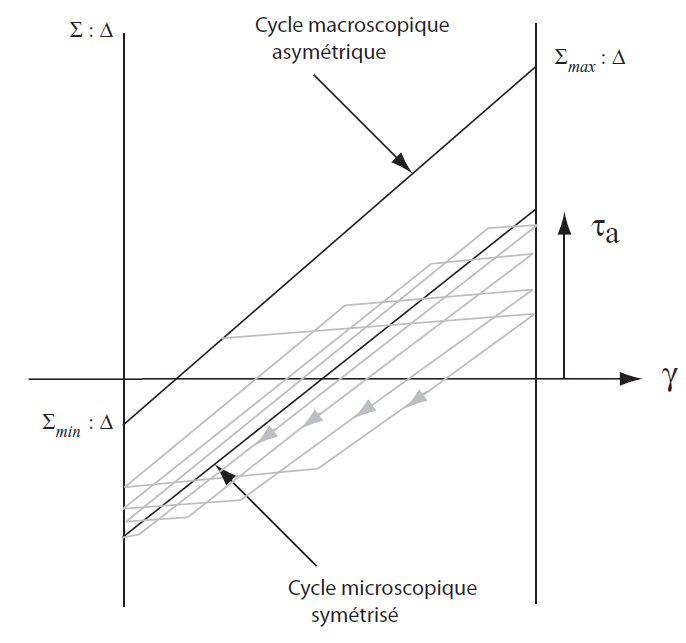
\includegraphics[width=0.7\textwidth]{figures//DV.png} 
	\caption{Elastic adaptation at the two scales [Dang Van 1999]}
	\label{figDV}
\end{figure}
Finally, a micro to macro is applied to determine the criteria on the macroscopic scale. The localization law used is
Lin-Taylor model that assumes equality of deformations at two scales. Using empirical relationships, the harmful role of the mean stress on the fatigue
strength of the material is shown for type of uniaxial tensile stress. Dang Van shows the effect of the mean stress
with  hydrostatic stress term in the criteria expressed as a linear combination of mesoscopic  shear stress on the maximum shear plane $\tau_a$ and the hydrostatic stress $\Sigma_h$.


The Dang Van criterion presented in \cite{ballard1995high} is expressed as:
\begin{equation}
	\max \limits_{\vec{n}}\left\lbrace \max \limits_{t}\left\{\tau_a{(\vec{n},t)}+a_D\Sigma_h(t)\right\}\right\rbrace \leqslant b_D.
	\label{dv}
\end{equation}

$\tau_a$ denotes the mesoscopic shear stress amplitude and is obtained from a mesoscopic stress tensor $\hat{\bm{\sigma}}$ defined by:
$$\hat{\bm{\sigma}}(t)=(\bm{\sigma}(t)-s^\star).$$
$s^\star$ is the center of the smallest hypersphere circumscribed to the loading path in deviatoric stress space. It is obtained by solving a ``min-max" problem as follows:
$$s^\star = arg \min\limits_{s_1}\left\{\max\limits_t\parallel s(t)-s_1\parallel\right\}.$$
In the case of fully reversed loading, the values $s^\star=0$ can be directly deduced without solving the ``min-max problem" as in general case.

The principal stress values of stress tensor $\widetilde{\sigma}$ denoting by $\hat{\sigma}_{\Rmnum{3}}(t)\leqslant\hat{\sigma}_{\Rmnum{2}}(t)\leqslant\hat{\sigma}_{\Rmnum{1}}(t)$, one gets the amplitude of shear stress by:
$$\tau(t)=\frac{1}{2}(\hat{\sigma}_{\Rmnum{1}}(t)-\hat{\sigma}_{\Rmnum{3}}(t)).$$
$\Sigma_h(t)$is the hydrostatic stress as a function of the time, given by:$$\Sigma_h(t)=\frac{\sigma_{kk}(t)}{3}.$$
The material characteristic parameters $a_D$ and $b_D$ of the Dang Van
criterion, can be related to the fully reversed bending (or tension-
compression because of the same stress state between them)fatigue limit, denoted by $f_{-1}$ (or $S_{-1}$), and to the torsion fatigue limit, denoted by $t_{-1}$,

$$a_D=\frac{3t_{-1}}{s_{-1}}-\frac{3}{2};$$  $$b_D=t_{-1}.$$

In the particular case of the uniaxial tension, the criterion is written as:
$$\Sigma_{xx,a}\left(\dfrac{1}{2}+\dfrac{a_D}{3} \right)+\Sigma_{xx,m}\left(\dfrac{a_D}{3} \right) =b_D$$

\textbf{Papadopoulos Criterion}

The approach proposed by \cite{papadopoulos1993fatigue} also uses the concept of elastic adaptation and even the localization law. According to him, "the observations at the mesoscopic scale show that the initiation of a fatigue crack is
defined as the occurrence of micro-cracks corresponding to the rupture of the most deformed crystal grains in an
aggregate. Thus, a fatigue limit criterion can be modeled by a limit value of the accumulated plastic strain in the
most distorted grain."
$$\gamma_{cum}\leqslant\gamma_\infty$$
He proposes to opt for a mean value of the accumulated plastic strain on all possible slip systems of representative elementary volume(REV). So he chose to use a average value  of accumulated plastic deformation rather than looking at failure of a single crystal. A spherical coordinate system(\figref{fig50}) to guide the vector of normal in material plane, and the unit direction vector $r$ linked to a sliding direction of this plan is used to conduct the integration over all possible orientations.

         \begin{figure}[h!]
         	\centering
         	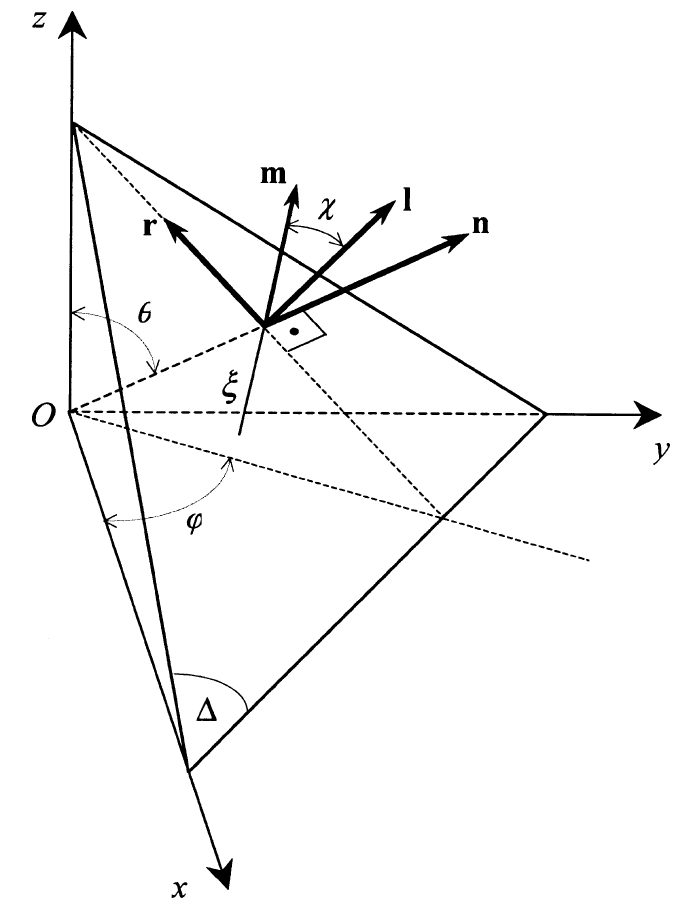
\includegraphics[width=0.5\textwidth]{figures//demopp.png} 
         	\caption{Material plane $\Delta$ passing through point O of a body and its
         		associated (n, l, r) frame.}
         	\label{fig50}
         \end{figure}
         At any point $O$ of a body, a material plane $\Delta$ can be defined by its unit normal vector $\bf n$. This vector
         $\bf n$ makes an angle $\theta$ with the z-axis of a $Oxyz$ frame attached to the body, and its projection on the $xy$ plane
         makes an angle $\varphi$ with axis $x$. For each plane $\Delta$ a new quantity is introduced called $generalised$ $shear$ $stress$ amplitude and denoted as $T_a$.This shear stress quantity was first introduced in Papadopoulos [6]
         and was subsequently used by other researchers.The critical plane according to our proposal is that onto which $T_a(\varphi,\theta)$ achieves its maximum value. The fatigue limit criterion is written as:
         \begin{equation}
         	max T_a+\alpha_\infty \Sigma_{h,max}\leqslant \gamma_\infty
         \end{equation}
         where $\alpha_\infty$ and $\gamma_\infty$ are material parameters to be determined\cite{papadopoulos2001long}.
         $$\Sigma_{h,max}=\max\limits_{t}\left\lbrace \frac{1}{3}tr(\uline{\uline{\sigma}}(t))\right\rbrace $$
         He introduced the resolved shear stress $\tau$:
         \begin{equation}
         	\begin{split}
         		\tau=&[sin\theta cos\varphi\sigma_{xx}+sin\theta sin\varphi\sigma_{xy}+cos\theta\sigma_{xz}](-sin\varphi cos\chi-cos\theta cos\varphi sin\chi)+\\&[sin\theta cos\varphi\sigma_{xy}+sin\theta sin\varphi\sigma_{yy}+cos\theta\sigma_{yz}](cos\varphi cos\chi-cos\theta sin\varphi sin\chi)+\\&[sin\theta cos\varphi\sigma_{xz}+sin\theta sin\varphi\sigma_{yz}+cos\theta\sigma_{zz}]sin\theta sin\chi
         	\end{split} 
         	\label{eqres}
         \end{equation}
         It is clear that the resolved shear stress is a function of
         $\varphi$, $\theta$, $\chi$ and of time $t$ in the case of variable loading, i.e. $\tau=\tau(\varphi, \theta, \chi, t)$. Upon fixing a couple $(\varphi, \theta)$ (i.e. a plane
         $\Delta$) and an angle $\chi$ (i.e. a line $\xi$ on $\Delta$), one can define the amplitude of the resolved shear stress $\tau_a$, acting on $\Delta$
         along $\xi$ by the formula:
         \begin{equation}
         	\tau_a(\varphi,\theta,\chi)=\frac{1}{2}\big[\max \limits_{t\in P}\tau_a(\varphi,\theta,\chi ,t)-\min \limits_{t\in P}\tau_a(\varphi,\theta,\chi ,t)\big]
         \end{equation}
         Finally, for a given plane $\Delta$, i.e. for a fixed couple ($\varphi$, $\theta$),
         the generalized shear stress amplitude $T_a$ is defined as:
         \begin{equation}
         	T_a(\varphi,\theta)=\sqrt{\frac{1}{\pi}\int_{x=0}^{\frac{\pi}{2}} \tau_a^2(\varphi,\theta,\chi)d\chi}
         	\label{Ta}
         \end{equation}
         We note the fatigue limit in fully reversed torsion $t_{-1}$ and the fatigue limit in fully reversed bending $f_{-1}$. From these two tests we get the parameters:
         $$\gamma_\infty=t_{-1},$$ 
         $$\alpha_\infty=3\left( \frac{t_{-1}}{f_{-1}}-\frac{1}{2}\right) .$$
         The Papadopoulos fatigue limit criterion achieves the form:
         \begin{equation}
         	maxT_a+3\left( t_{-1}/f_{-1}-1/2\right) \Sigma_{h,max}\leqslant t_{-1}.
         	\label{eq:papadopoulos}
         \end{equation}
         In the particular case of the uniaxial tension, the criterion is written as:
         $$\Sigma_{xx,a}\left(\dfrac{1}{\sqrt{3}}+\dfrac{\alpha_\infty}{3} \right)+\Sigma_{xx,m}\left(\dfrac{a_\infty}{3} \right) =\gamma_\infty$$
         
\subsubsection{Criteria based on energy}
Depending on the type of density of deformation energy considered per cycle, the
Energy criteria are divided into three groups [Macha et al 1999]:
\begin{itemize}
	\item  criteria based on law of thermodynamics
	\item  criteria based on elastic energy
	\item  criteria based on plastic energy
	\item  criteria based on the sum of elastic and plastic energies
\end{itemize}

The criteria based on the elastic deformation energy can be used in fatigue with a large number of cycles, whereas those based on the plastic deformation energy are more suitable for oligocyclic fatigue.

[Ellyin 1974]\cite{Ellyin1974} is one of the first to propose a fatigue criterion based on cyclic shear deformation energy. This approach was taken up and complemented by [Lefebvre et al 1981]\cite{neale1981criterion} and [Ellyin et al., 1991]\cite{ellyin1991phase} for the case of multiaxial loadings. In France, this approach is reflected in the work of [Froustrey-Lasserre 1992]\cite{Froustey1992} and then in [Palin-Luc 1996]\cite{palin1996fatigue} and [Banvillet 2001]\cite{vidal1996prevision}.

\paragraph{Energy dissipation based on law of thermodynamics}

         In case of shell model. We assume the temperature in the thickness direction does not change. Based on the first and second law of thermodynamics, for any point M, we define $T(M,t)$ is the temperature field of $M$ at time $t$. Its 2D heat transfer function is \cite{yuan2013prediction}:
         $$\rho C \frac{\partial T(M,t)}{\partial t}-k\Delta_2 T(M,t)+\frac{2\sigma_e\varepsilon_mT(M,t)^4}{e}+\frac{2h}{e}[T(M,t)-T(M,t)^{air}]=d_1(M,t)+S_{th}(M,t)+r(M,t)$$
         
         $\rho$ is the density of the steel, C is specific heat capacity, k is heat transfer coefficient, $\sigma_e$ is the bolzmann constant, $\varepsilon_m$ is the surface thermal emissivity, h is heat convection factor,$T(M,t)^{air}$ is the environment temperature at point M, $\Delta_2$ is two dimensional Laplace operator.  $d_1(M,t)$ is the dissipative source of fatigue relevant irreversible strain $\varepsilon_{ir}$, strain hysteresis $\varepsilon_{ve}$ and micro structure deformation; $S_{th}(M,t)$ is the thermoelastic source composing of elastic strain $\varepsilon_e$; $r(M,t)$ is thermal radiation term.
         
         In a single cycle the dissipated energy is only a function of dissipative source $d_1(M,t)$:
         
         $$E_{d_1}(t)=\int_{t-\frac{t_f}{2}}^{t+\frac{t_f}{2}}d_1(t)dt$$
         
         Experiments with different stress amplitude loadings shows that the correlation coefficient between dissipated energy in one cycle and fatigue life is more than S-N curve.
         
         $lgE_{d_1}^m=-0.77lgN_F+8.33$ correlation coefficient:0.94
         
         $lg\sigma_a=-0.13lgN_F+2.85$ correlation coefficient:0.89
         
         
\paragraph{Energy dissipation based on strain energy density}

         In their fatigue criterion, Froustey et al. (1992)  have considered a complete cycle of
         stresses. They use the mean value on one cycle of
         the volumic density of the elastic strain energy, $W_a$, whatever the point
         M in the mechanical part.
         
         $$W_a(M)=\frac{1}{T}\int_{0}^{T}\frac{1}{2}\sigma_{ij}(M,t)\varepsilon_{ij}^e(M,t)dt$$
         
         where $\sigma_{ij}(M,t)$ and $\varepsilon_{ij}^e(M,t)$ are respectively the tensor of stresses and the tensor of
         elastic strains at the considered point $M$ function of time $T$.Usually the endurance limit
         is low enough to consider that the material remains elastic at the macroscopic scale
         (Lemaitre and Chaboche, 1988). Thus, $W_a$ can be considered as the mean value on one
         cycle of the total strain energy density at the considered point.
         
         In 1998 Thierry PALIN-LUC and Serge LASSERRE \cite{palin1998energy} proposed the failure criterion of $W_a$:
         
         Their studies show that another limit, called $\sigma^*$, can be defined below
         the usual endurance limit of the material, $\sigma_D$. At a considered point a stress amplitude
         below this new limit does not initiate observable damage at the microscopic scale (no
         micro-cracks).
         
         From $\sigma^*$ and by analogy with a sinusoidal traction load the corresponding mean value
         of the strain energy volumetric density, $W_{a^*}$, can be calculated , where E is the
         Young modulus of the material.
         
         $$W_{a^*}=\frac{\sigma^{*2}}{4E}$$
         
         Around each point it is always possible to define
         the volume $V^* (C_i)$ by the set of points M where $W_a (M)$ is higher than $W_{a^*} (C_i)$
         . They postulate that the part of $W_a (M)$ exceeding $W_{a^*} (C_i)$ is the damaging part
         of the strain energy volumetric density.  $\overline{\omega}_a(C_i)$ is
         the volumetric mean value of the strain energy around the critical point $C_i$
         
         $$V^*(C_i)=\lbrace points\, M(x,y,z) \,around\, C_i \,such\, that \,W_a(M)\geqslant W_{a^*}(C_i) \rbrace$$
         
         $$\overline{\omega}_a(C_i)=\frac{1}{V^*(C_i)}\int\int\int_{V^*(C_i)}^{}[W_a(x,y,z)-W_{a^*}(C_i)]d\nu$$
         
         This stress limit $\sigma^*$ can be estimated from
         fatigue test results in fully reversed tension and in rotating
         bending
         
         $$\sigma^*=\sqrt{2(\sigma_{Ten,-1}^D)^2-(\sigma_{RotBend,-1}^D)^2}$$
         
         
\paragraph{A critical plane approach based on energy concepts}
In 1999 Tadeusz et al.\cite{lagoda1999critical} proposed under multiaxial loadings the normal strain energy density in the critical plane (i.e. the plane of the maximum damage) is understood as the energy parameter. The history of strain energy density is schematized with use of the rain-flow algorithm. Fatigue damage is accumulated according to Palmgren-Miner hypothesis and the standard fatigue characteristic of the material, rescaled with use of the considered energy parameter. 
         $$W(t)=\frac{1}{2}\sigma(t)\varepsilon(t)sgn[\sigma(t),\varepsilon(t)]$$
         $$sgn(x,y)=\frac{sgn(x)+sgn(y)}{2}$$
         
         $sgn(x),sgn(y)=0,1,-1$ for distinguishing positive and negative works in a
         fatigue cycle.
         
         If the stress and strain reach their maximum values,
         $\sigma_a$ and $\varepsilon_a$, then the maximum energy density value is
         $$W_a=\frac{1}{2}\sigma_a\varepsilon_a$$
         
         In the case of high-cycle fatigue,
         when the characteristic ($\sigma_a-N_F$) is used, the axis $\sigma_a$
         should be replaced by $W_a$, where
         
         $$W_a=\frac{\sigma_a^2}{2E}$$
         
         In the case of low and high-cycle fatigue, when the
         characteristic ($\varepsilon_a-N_F$) is used, we can do similar rescaling. We assume $$\sigma_a=\sigma_f'(2N_F)^b$$
         
         From Manson-Coffin-Basquin equation we obtain
         
         $$\varepsilon_a=\varepsilon_a^e+\varepsilon_a^p=\frac{\sigma_f'}{E}(2N_F)^b+\varepsilon_f'(2N_F)^c$$
         $$W_a=\frac{1}{2}\sigma_a\varepsilon_a=\frac{\sigma_a}{2}\left[\frac{\sigma_f'}{E}(2N_F)^b+\varepsilon_f'(2N_F)^c\right]=\frac{(\sigma_f')^2}{2E}(2N_F)^{2b}+0.5\varepsilon_f'\sigma_f'(2N_F)^{b+c}$$
         
         Fatigue characteristic for high-cycle fatigue
         takes the form
         $$W_a=\frac{(\sigma_f')^2}{2E}(2N_F)^{2b}$$
         
         For the stress model we have:
         
         $$lgN_F=A-mlg\sigma_a$$
         
         For the energy model we have:
         $$lgN_F=A'-m'lgW_a$$
         $m'$ is slope of fatigue curve
         expressed by energy.

\paragraph{Lamefip Criterion}
Ellyin\cite{ellyin2012fatigue} showed that the use of both the plastic and elastic strain work can be used
as damage parameter in multiaxial fatigue. The LAMEFIP criterion (Banvillet et al. [2003]\cite{banvillet2003volumetric}),
devoted to the field of endurance or limited endurance, uses for damage parameter, the volumetric density of the strain work given to the material per loading cycles after elastic shakedown(supposed to be reached after a few thousands cycles ).

The proposal is based on two main hypothesis : (i) the strain work given to the material per loading cycle is considered as the driving force for fatigue crack initiation and (ii) it is calculated after macroscopic elastic shakedown.

Many authors use cycle counting techniques to extract, from a random stress tensor sequence, cycles from which the damage could be estimated. These techniques have two main drawbacks : (i) the choice of the cycle counting algorithm influences the calculated fatigue life since the number of counted cycles is algorithm dependent (Dowling [1983]\cite{dowling1983fatigue}), and (ii) for multiaxial non-proportional stress states, in many approaches from the literature, the variable chosen for cycle counting differs from the damage parameter. To avoid such drawbacks an incremental model has been developed. The strain work density given at a point M is written in an incremental way as follows :

$$dW_g(M,t)=\sum_{i=1}^{3}\sum_{j=1}^{3}\sigma_{ij}\left( M,t\right)\dot{\epsilon}_{ij}\left( M,t\right)H\left( \sigma_{ij}\left( M,t\right),\dot{\sigma}_{ij}\left( M,t\right)\right)dt .$$

\noindent
- where $\epsilon_{ij}\left( M,t\right)$ are the strain tensor components and $\dot{x}= dx/dt$,\\
- $\sigma_{ij}\left( M,t\right)$ are the stress tensor components,\\
- and H represents the Heaviside function : $H(a) = 1$ if $a \geqslant 0$; $H(a) = 0$ if $a < 0$.

As underlined by Ellyin\cite{ellyin2012fatigue}, the strain work can be calculated as the sum of elastic and plastic strain works, so that :
$$dW_g(M,t)=dW_g^e(M,t)+dW_g^p(M,t).$$
The framework of this study being HCF and MCF, they choose to consider only the elastic part of the strain work (Eq.\eqref{eq.lamefip1}) in the elastic shakedown state. The cumulated strain work on a time
sequence of duration $T$ is equivalent to the integral of $dW_g^e(M,t)$ over $T$ as in Eq.\eqref{eq.lamefip2}. Banvillet et al. [2003]\cite{banvillet2003volumetric} has shown that for an uniaxial stress state $W_g$ is not shape dependent (sinus, triangle,square, etc...).
\begin{equation}
dW_g^e(M,t)=\sum_{i=1}^{3}\sum_{j=1}^{3}\sigma_{ij}\left( M,t\right)\dot{\epsilon}_{ij}^e\left( M,t\right)H\left( \sigma_{ij}\left( M,t\right),\dot{\sigma}_{ij}\left( M,t\right)\right)dt .
\label{eq.lamefip1}
\end{equation}
\begin{equation}W_g(M,t)=\int_{T}dW_g(M,t).\label{eq.lamefip2}
\end{equation}

To take into account the material sensitivity to the stress triaxiality, the triaxiality degree at a point M is defined by the ratio of the strain work associated with the spherical part of the stress tensor over the total given in the work of Banvillet et al.[2003]\cite{banvillet2003volumetric}, but in an incremental way :
$$dT(M,t)=\dfrac{dW_g^{Sph}(M,t)}{dW_g(M,t)} \ \ if \ \  dW_g(M,t)\neq0,\ otherwise \ \ dT(M,t)=0,$$
with
$$dW_g^{Sph}(M,t)=\dfrac{1}{3}\sum_{k=1}^{3}\sigma_{kk}(M,t)\sum_{l=1}^{3}\dot{\epsilon}_{ll}^e(M,t)H\left( \sum_{k=1}^{3}\sigma_{kk}(M,t)\sum_{l=1}^{3}\dot{\epsilon}_{ll}^e(M,t)\right)dt .$$
The material sensitivity to stress triaxiality is considered by using an empirical function
$F(dT,\beta_m)$ (Eq.\eqref{eq.lamefip3}) depending on the material parameter $\beta_m$ identified from two fully reversed
fatigue limits (rotating bending and torsion). At any instant, for a multiaxial stress state, the
strain work given to the material is corrected to evaluate an uniaxial equivalent strain work
$d{W_f}_{eq} (M,t)$ (Eq.\eqref{eq.lamefip4}). Under uniaxial stress state $d{W_g}_{eq} (M,t)=dW_g(M,t)$.
\begin{equation}
F(dT(M,t),\beta_m)=\dfrac{1}{1-dT(M,t)}\left[ 1-\dfrac{1}{\beta_m}ln\left[1+dT(M,t)(e^{\beta_m}-1) \right] \right] .
\label{eq.lamefip3}
\end{equation}
\begin{equation}
d{W_g}_{eq} (M,t)=d{W_g}(M,t)\dfrac{F(dT_{uniax,\beta_m})}{F(dT(M,t),\beta_m)}.
\label{eq.lamefip4}
\end{equation}

\subsubsection{Criteria based on plasticity-damage coupling}
In recent years, a new class of criteria coupling mesoplasticity and damage has emerged. [Lemaitre Sermage Desmorat 1999]\cite{lemaitre1999two} have, for example, evolved the approach introduced by [Lemaitre and Chaboche 1985]\cite{lemaitre1985mecanique} based on the thermodynamics of irreversible processes and the mechanics of continuous media. [Flaceli{\`e}re et al. 2004]\cite{flaceliere2004contribution} also proposed a model based on a plasticity-damage coupling and attempted to account for the phenomena of damage observed experimentally on a C35 steel. In this work, we will focus on a more recent approach proposed by [Monchiet et al 2006]\cite{monchiet2006contributions}.
\paragraph{Criterion of Monchiet et al}
In order to account for the coupling plasticity-damage in HCF, [Monchiet et al. 2006]\cite{monchiet2006contributions} uses a micro-mechanical approach based on the work of [Gurson 1977]\cite{gurson1977continuum}. The damage is represented by a magnitude $f$ related to the development of porosity in the sliding bands at the origin of the initiation of the fatigue cracks. A load surface, of the type defined by Gurson, is used:
\begin{equation}
\dfrac{\Sigma_{equ}^2}{\Sigma_0^2}+2fcosh\left(\dfrac{3}{2}\dfrac{\Sigma_h}{\Sigma_0}-1-f^2=0 \right),
\label{eq.monchiet1}
\end{equation}
where $\Sigma_{equ}$ Is the equivalent stress, $\Sigma_h$ The hydrostatic stress and $\Sigma_0$ the elastic limit of the matrix.

The authors take into account two mechanisms of damage:

\vspace{6pt}
\begin{itemize}
	\item  The first is related to the creation of gaps by annihilation of dislocations. This mechanism is at the origin of the accumulation of point defects of the lacunar or interstitial type along the persistent slip bands (PSB). The phenomenological model proposed by [Essmann et al 1979]\cite{doi:10.1080/01418618108239541} gives access to the porosity $f_a$:
\begin{equation}
f_a= A_0\left\lbrace k_a\gamma_{cum}-1+exp\left(-k_a\gamma_{cum} \right)  \right\rbrace .
\label{eq.monchiet2}
\end{equation}

	\item  The second mechanism is related to the growth of micro-cavities. Using an incompressibility hypothesis, $f_g$ is defined by:
\begin{equation}
f_g=\left\lbrace 1-exp\left(3\epsilon_h^p \right) \right\rbrace.
\label{eq.monchiet3}
\end{equation}
\end{itemize}

	It is important to note that the first mechanism involves the accumulated plasticity $\gamma_{cum}$, related to amplitude effects. The second mechanism depends on the hydrostatic plastic deformation $\epsilon_h^p$, and allows the taking into account of the mean stress effects.
	
	The fatigue criterion is established on the basis of the following hypothesis: "a sufficient condition for nucleation of a fatigue crack is obtained if the porosity reaches a critical value $f_c$".
	\begin{equation}
	f\left( \gamma_{cum},\epsilon_h^p\right) =f_a+f_g\leqslant f_c.
	\label{eq.monchiet4}
	\end{equation}

Noting $\gamma_c$, the critical value of the cumulative plasticity for which the fatigue criterion is reached when $\epsilon_h^p=0$, it becomes:
\begin{equation}
f_c=\left\lbrace A_0\left\lbrace k_a\gamma_{c}-1+exp\left(-k_a\gamma_{c} \right)  \right\rbrace \right\rbrace.
\label{eq.monchiet5}
\end{equation}
The use of Eq.\eqref{eq.monchiet4} and Eq.\eqref{eq.monchiet5} leads, for the limiting cases $k_a >> 1$ Eq.\eqref{eq.monchiet6}, $k_a << 1$ Eq.\eqref{eq.monchiet7}, noting $\epsilon_c$(The critical plastic deformation, equal to $f_c / 3$ in the case of $\gamma_{cum} 0$), there is:
\begin{equation}
\dfrac{\gamma_{cum}}{\gamma_{c}}+\dfrac{\epsilon_h^p}{\epsilon_c}=1,
\label{eq.monchiet6}
\end{equation}
\begin{equation}
\left( \dfrac{\gamma_{cum}}{\gamma_{c}}\right) ^2+\dfrac{\epsilon_h^p}{\epsilon_c}=1.
\label{eq.monchiet7}
\end{equation}

The effect of the mean stress is taken into account by the term hydrostatic deformation. Since $\gamma_{cum}$ and $\epsilon_h^p$ are defined on the grain scale, the macroscopic expression of the criterion requires to link these quantities to the macroscopic magnitudes of the loading.

The next step is to look for elastic adaptation conditions and to apply a micro-macro path. The numerical results obtained make it possible to establish the following relations between the loading parameters and the parameters of the local criterion:

\begin{equation}
\left( \dfrac{T_a}{\tau_d}\right) ^2+2f_ccosh\left\lbrace\dfrac{\sqrt{3}}{2}\dfrac{\Sigma_{h,a}}{\tau_h} \right\rbrace-1-f_c^2=0.
	\label{eq.monchiet8}
\end{equation}
\begin{equation}
\Sigma_{h,m}=-\left( \dfrac{4c}{f_cln(f_c)}\left( 1-f_c\right)+3k^{\ast} \right) \epsilon_h^p.
	\label{eq.monchiet9}
\end{equation}

In Eq.\eqref{eq.monchiet8}, $\tau_d$ and $\tau_h$ are the deviatoric and hydrostatic part of the plastic flow threshold associated with an isotropic hardening.

In Eq.\eqref{eq.monchiet8}, $c$ and $k^{\ast}$ are parameters related respectively to the kinematic hardening and to the homogenization scheme.

The implementation of this criterion requires the identification of 12 parameters:
\begin{flushleft}
\qquad - \qquad two parameters, $\gamma_c$ and $\epsilon_c$ linked to the local criterion.\\
\qquad - \qquad two parameters, $A_0$ and $k_a$, related to the mechanisms of nucleation of cracks.\\
\qquad - \qquad three parameters related to hardening, $R_0$ And $\tau_0$ linked to the isotropic hardening, $c$ linked to\\
\qquad  \ \   \qquad   the kinematic hardening\\
\qquad - \qquad two coefficients linked to the homogenization scheme, $\mu$ and $k$.\\
\qquad - \qquad a cubic anisotropy coefficient of the grain $p_1$\\
\qquad - \qquad a latent coefficient of strain hardening h\\
\qquad - \qquad a critical porosity coefficient $f_c$\\
\end{flushleft}

All of these parameters are microscopic, which poses a problem in their identification. Some elements of this modeling have been taken up by [Charkaluk and Constantinescu 2009]\cite{charkaluk2009revisiting}, [Charkaluk et al. 2007]\cite{charkaluk2007approche} in dissipative approaches.





\subsection{Basquin curve}

\vspace{6pt}
\textbf{Stress-Life Diagram (S-N Diagram)}

The basis of the Stress-Life method is the Wohler S-N diagram, shown schematically for two
materials in \figref{fig.sn}. The S-N diagram plots nominal stress amplitude S versus cycles to
failure N. There are numerous testing procedures to generate the required data for a proper
S-N diagram. S-N test data are usually displayed on a log-log plot, with the actual S-N line
representing the mean of the data from several tests.

\begin{figure}[!h]
	\centering
	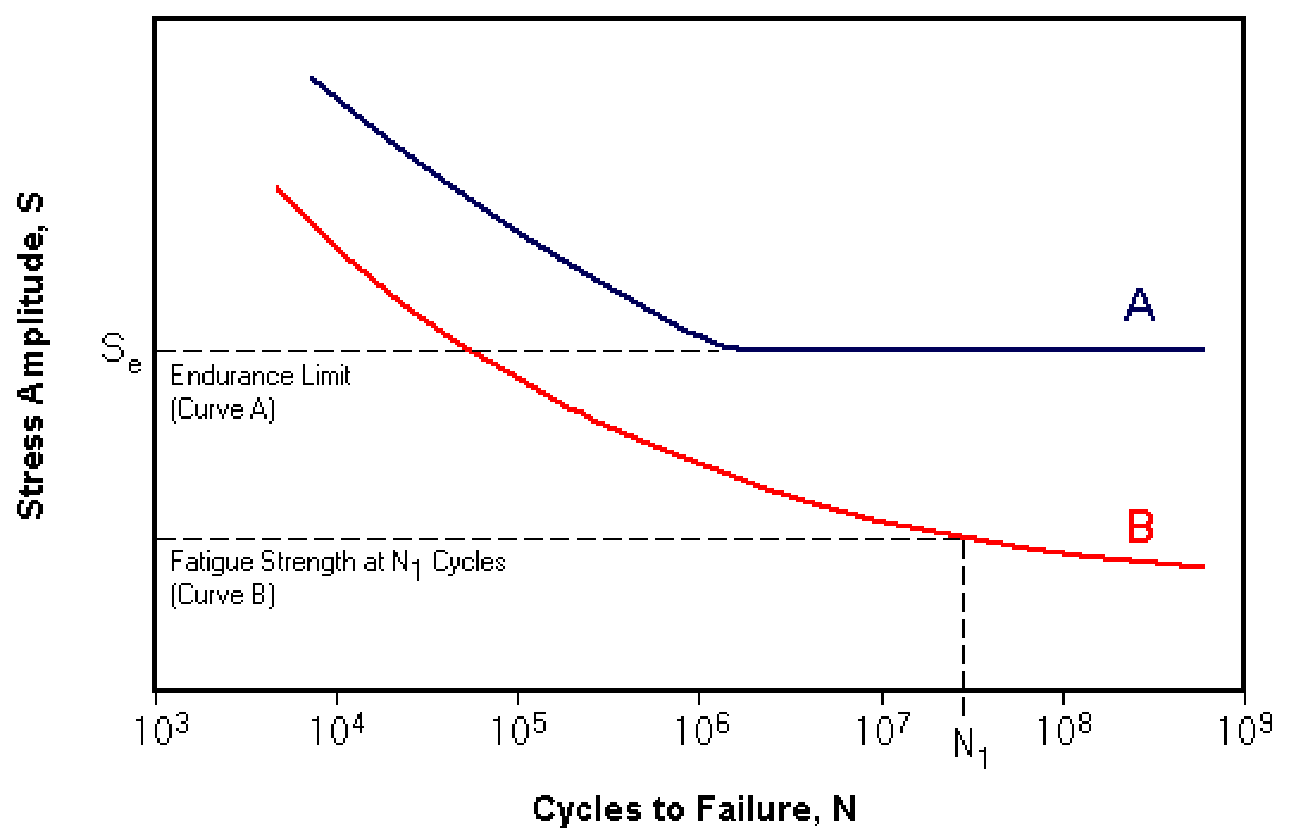
\includegraphics[width=0.7\textwidth]{figures//sn.png} 
	\caption{Typical S-N curve.}
	\label{fig.sn}
\end{figure}

\textbf{Endurance Limit}

Certain materials have a fatigue limit or endurance limit which represents a stress level below
which the material does not fail and can be cycled infinitely. If the applied stress level is below
the endurance limit of the material, the structure is said to have an infinite life. This is
characteristic of steel and titanium in benign environmental conditions. A typical S-N curve
corresponding to this type of material is shown Curve A in  \figref{fig.sn}.

Many non-ferrous metals and alloys, such as aluminum, magnesium, and copper alloys, do not
exhibit well-defined endurance limits. These materials instead display a continuously
decreasing S-N response, similar to Curve B in \figref{fig.sn}. In such cases a fatigue strength $S_f$ for
a given number of cycles must be specified. An effective endurance limit for these materials is
sometimes defined as the stress that causes failure at $1x10^8$ or $5x10^8$ loading cycles.

The concept of an endurance limit is used in infinite-life or safe stress designs. It is due to
interstitial elements (such as carbon or nitrogen in iron) that pin dislocations, thus preventing
the slip mechanism that leads to the formation of microcracks. Care must be taken when
using an endurance limit in design applications because it can disappear due to:

\vspace{6pt}
$\bullet$ Periodic overloads (unpin dislocations)

$\bullet$ Corrosive environments (due to fatigue corrosion interaction)

$\bullet$ High temperatures (mobilize dislocations)
\vspace{6pt}     

The endurance limit is not a true property of a material, since other significant influences such
as surface finish cannot be entirely eliminated. However, a test values ($S_e'$) obtained from
polished specimens provide a baseline to which other factors can be applied. Influences that
can affect the endurance limit include:

\vspace{6pt}
$\bullet$ Surface Finish

$\bullet$ Temperature

$\bullet$ Stress Concentration

$\bullet$ Notch Sensitivity

$\bullet$ Size

$\bullet$ Environment

$\bullet$ Reliability
\vspace{6pt}         

\textbf{Power Relationship}   

When plotted on a log-log scale, an S-N curve can be approximated by a straight line as shown
in \figref{fig.basquin}. Basquin’s equation is a power law relationship\ref{eq.basquin} which describes the linear relationship between the applied stress cycles (S) in the y-axis and the number of cycles to failure in the x-axis plotted on a log-log scale.
\begin{equation}
	N=BS^\frac{1}{b}
	\label{eq.basquin}
\end{equation}
To calculate the slope of the Basquin equation, solve the system of equations:
$$N_1=N_2\left(\dfrac{S_1}{S_2}\right)^\frac{1}{b},$$
$$b=\dfrac{logS_1-logS_2}{logN_1-logN_2},$$
where $b$ is the slope of the line.
$$B=N_1S_1^{-\frac{1}{b}}=N_2S_2^{-\frac{1}{b}}.$$
For the constant B, in industry  the stress range value (from the maximum cyclic stress to the minimum cyclic stress) is often considered. If the stress values of the S-N curve are given as alternating stresses (which is the common practice), multiply these stresses by 2 to calculate the constant B (stress range = 2* alternating stress, assuming a zero mean stress and full reversal of the cyclic load). If the S-N curve data are given in stress range values, apply them directly in the equation for estimating the constant B. 

\begin{figure}[h!]
	\centering
	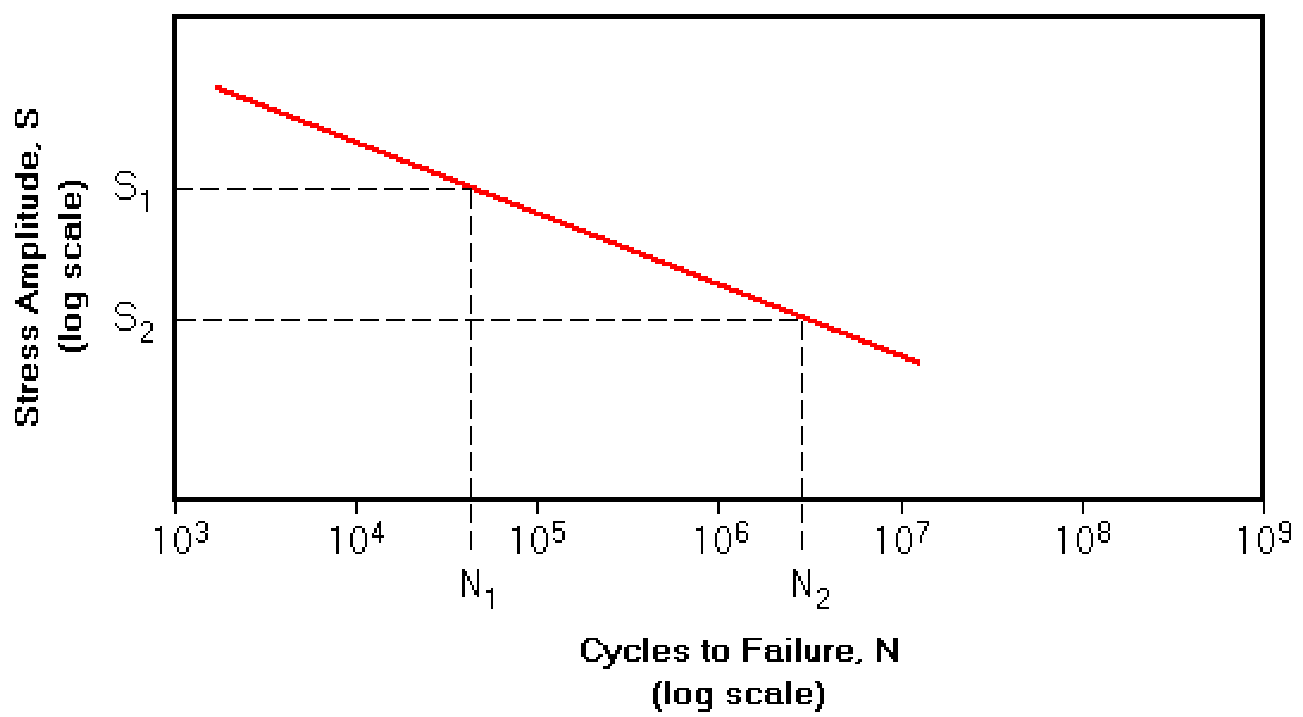
\includegraphics[width=0.7\textwidth]{figures//basquin.png} 
	\caption{Idealized S-N curve for high cycle fatigue.}
	\label{fig.basquin}
\end{figure}

The power relationship is only valid for fatigue lives that are on the design line. For ferrous metals this range is from $1x10^3$ to $1x10^6$ cycles. For non-ferrous metals, this range is from
$1x10^3$ to $5x10^8$ cycles. 
         
\subsection{Calculation method without cycle counting}
This part presents the existing method of prediction of lifetime, which does not need the algorithm of cycle counting. These kind of methods are still minority and usually more delicate to implement, but present the advantage of free the choice of variable of counting proved to be ``dangerous''. The method presented here is the morel method which is based on stress.

\subsubsection{Morel's method}
Morel's method\cite{Morel2000101} is based on a mesoscopic approach to critical plane type with the
choice of plastic deformation as mesoscopic cumulative damage variable.  Multiaxial and variable amplitude loading can be analyzed with this method.
\begin{flushleft}
Macroscopic quantities
\begin{table}[!h]
	\begin{tabular}{lllll}
		$\uline{\uline{\Sigma}}$ & macroscopic stress tensor &  &  &  \\
		$\uline{\uline{E}}$ & macroscopic strain tensor &  &  &  \\
		$\uline{\uline{C}}$ & macroscopic shear stress vector  &  &  &  \\
		$\uline{\uline{T}}$ & macroscopic resolved shear stress vector acting on an easy glide direction&  &  &  \\
		$T_a$ & amplitude of the macroscopic resolved shear stress  &  &  &  \\	
		$P$ & macroscopic hydrostatic stress &  &  &  \\	
	\end{tabular}
\end{table}

Mesoscopic quantities
\begin{table}[!h]
	\begin{tabular}{lllll}
		$\uline{\uline{\sigma}}$& mesoscopic stress tensor &  &  &  \\
		$\uline{\uline{\varepsilon}}$ & mesoscopic strain tensor &  &  &  \\
		$\uline{\tau}$& mesoscopic resolved shear stress vector acting on an easy glide direction &  &  &  \\
		$\gamma^p$& mesoscopic shear plastic strain &  &  &  \\
		$\Gamma$ & accumulated plastic mesostrain &  &  &  \\
		$T_\sigma$ & measure proportional to an upper bound of the plastic mesostrain accumulated on an elementary
		material plane $\Delta$, also average value of $T_a$ &  &  &  \\
		$T_\Sigma$ & maximum value of  $T_\sigma$&  &  &  \\
		$H$ & phase-difference coefficient&  &  &  \\
	\end{tabular}
\end{table}
\end{flushleft}

\textbf{Constant amplitude loading}
\vspace{6pt}

\textbf{Local stress estimation in high cycle fatigue}

By assuming that only one glide system (defined by a normal vector $\uline{n}$ to a plane and a vector
(direction) $\uline{M}$ within this plane) is active for every plastically deforming grain of the metal, Papadopoulos [9]
established a macro–meso passage for a glide system activated in a flowing crystal:
\begin{equation}
\uline{\tau}=\uline{T}-\mu\gamma^p\uline{m}
\label{macromeso}
\end{equation}
where $\uline{\tau}$ and $\uline{T}$ are the mesoscopic and macroscopic
resolved shear stresses acting along the slip direction $\uline{m}$ and defined by:
\begin{equation}
\uline{\tau}=(\uline{m}\cdot\uuline{\sigma}\cdot\uline{n})\uline{m}
\label{tau}
\end{equation}
\begin{equation}
\uline{T}=(\uline{m}\cdot\uuline{\Sigma}\cdot\uline{n})\uline{m}
\label{T}
\end{equation}
$\gamma^p$  is the plastic mesoscopic shear strain.
\begin{figure}[h!]
	\centering
	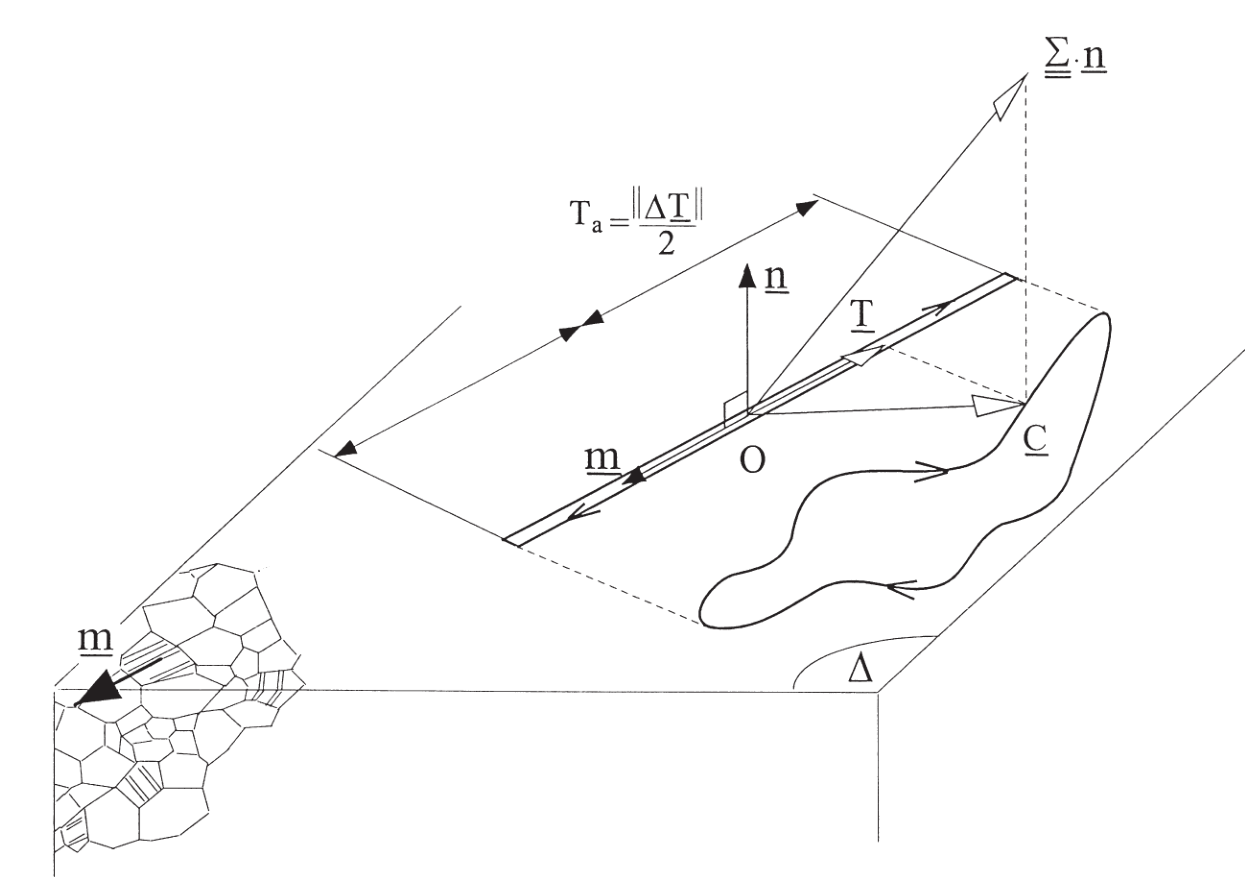
\includegraphics[width=0.8\textwidth]{figures//glid.png} 
	\caption{Path of the macroscopic shear stress $\uline{C}$ acting on a material plane $\Delta$ and the corresponding path of the macroscopic resolved shear stress $\uline{T}$ acting on an easy glide direction.}
	\label{glid}
\end{figure}

\textbf{Initiation of slip in the crystal}

The plasticity criterion is determined by Schmid's law with isotropic and kinematic hardening:
\begin{equation}
f(\uline{\tau},\uline{b},\tau_y)=(\uline{\tau}-\uline{b})\cdot(\uline{\tau}-\uline{b})-\tau_y^2=0
\label{Schmid}
\end{equation}
where $\uline{b}$ is the kinematical hardening parameter back stress.

In the description of his method, the author draws heavily on the work developed by
Papadopoulos including the use of a measure of plastic deformation mesoscopic
Cumulative $T_\sigma$ associated with a particular material plane and modeling the behavior of
grain in three distinct phases (hardening, saturation and softening); he considers the cumulative mesoscopic plastic deformation $\Gamma$ as damage parameter and assumes that the initiation of a fatigue crack occurs when the latter reaches a
critical value $D = D_R = \Gamma_R$ (\figref{3phases}). 
\begin{figure}[h!]
	\centering
	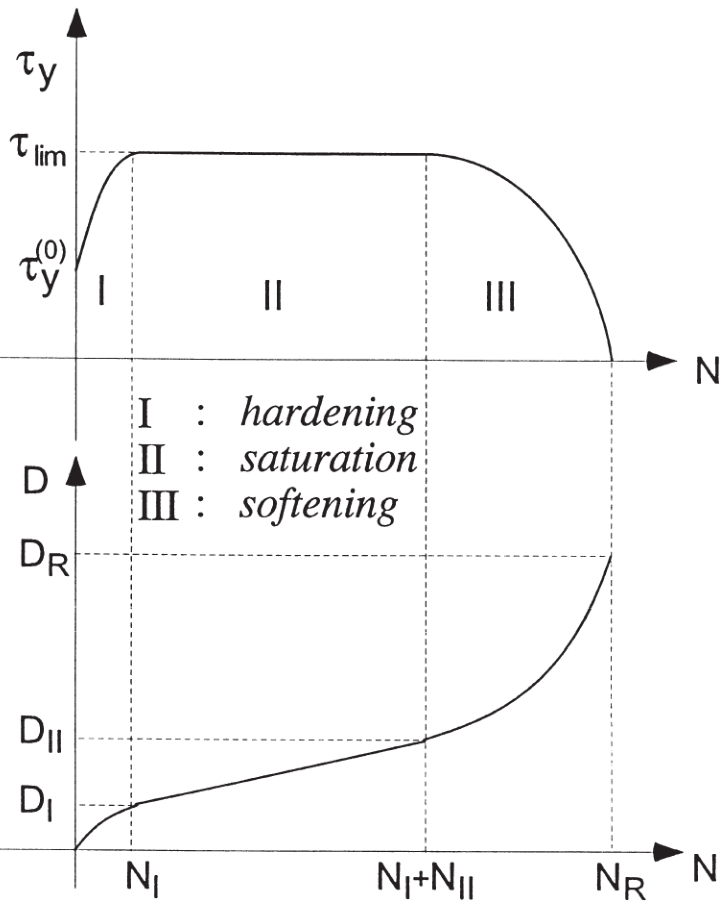
\includegraphics[width=0.5\textwidth]{figures//3phases.png} 
	\caption{Yield limit and damage evolutions in the three behavior phases (hardening, saturation and softening) when a cyclic loading	is applied.}
	\label{3phases}
\end{figure}

\textbf{Loading limit estimation}

The estimation of the yield limit in the saturation phase $\tau_s$ (defining the cyclic behavior of the crystal) is
carried out by the definition of a limit loading.
\begin{equation}
T_{\Sigma lim}+\alpha P_{max lim}=\beta
\end{equation}
\begin{equation}
T_{\Sigma lim}=\frac{-\alpha P_m+\beta}{\alpha+\frac{T_\Sigma}{P_a}}\cdot\frac{T_\Sigma}{P_a}
\label{Tlim}
\end{equation}
Now we need to establish $\tau_{lim}$. The corresponding actual amplitude of the shear stress,
defined as half of the longest chord of the closed curve, is denoted as $C_A$.
\begin{equation}
H=\frac{T_{\Sigma}}{C_A}=\frac{T_{\Sigma lim}}{\tau_{lim}} \, \Rightarrow \, \tau_{lim}=\frac{T_{\Sigma lim}}{H}
\label{eqH}
\end{equation}
where H constitutes a ‘phase-difference coefficient’.
It is worth mentioning that the more open the elliptic
path, the higher the coefficient H. 

\begin{figure}[h!]
	\centering
	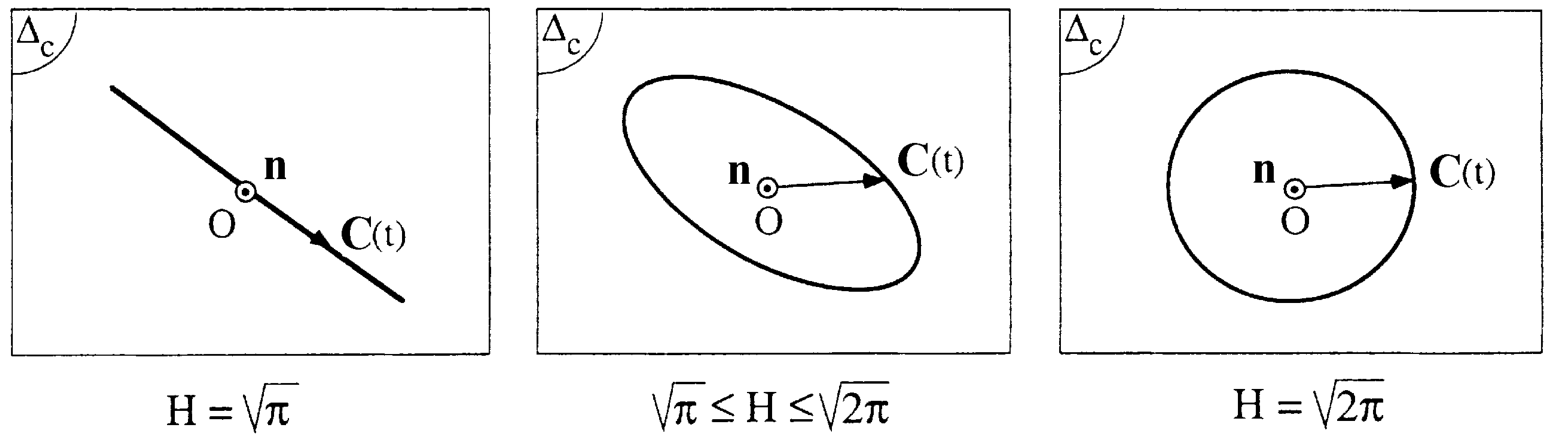
\includegraphics[width=0.9\textwidth]{figures//H.png} 
	\caption{Different paths and corresponding values of the phase-difference coefficient $H$.}
	\label{figH}
\end{figure}
For a proportional
loading, H is equal to $\sqrt{\pi}$. In the case of a particular
circular path, H reaches the maximum value $\sqrt{2\pi}$(\figref{figH}). 


\textbf{Number of cycles to failure}

Once the accumulated plastic mesostrain $\Gamma$ along the particular gliding
system reaches a critical value $\Gamma_R$, these grains are said
to be broken. An analytical expression of the number
of cycles to initiation (S–N curve) can be achieved:
\begin{equation}
\Gamma=\Gamma_R \, \Rightarrow \, N_F=pln\left(\frac{C_A}{C_A-\tau_{lim}}\right)+q\left(\frac{\tau_{lim}}{C_A-\tau_{lim}}\right)-\frac{r}{C_A}
\label{NF}
\end{equation}
where $p$, $q$ and $r$ are functions of the hardening parameters of the three phases defined above.

From Eq.\eqref{Tlim} and Eq.\eqref{eqH} we can find the yield point $\tau_s$ of the crystal in the saturation phase as a function of the amplitude $P_a$ and the mean value $P_m$ of the hydrostatic pressure, the phase difference of coefficient $H$ and two material related parameters $\alpha$ and $\beta$ :
\begin{equation}
\tau_{lim}=\tau_s=\frac{-\alpha P_m+\beta}{\alpha\frac{P_a}{C_A}+H}
\label{taus}
\end{equation}
In the last relation Eq.\eqref{NF}, the detrimental effect of out-of-phase loading is introduced through $\tau_{lim}$. As the coefficient $H$ increases, $\tau_{lim}$  decreases, therefore $N_F$ decreases which leads to more accumulated damage. The identification of the model parameters requires two endurance limits and a
single S–N curve (parameters $p$, $q$ and $r$).



\textbf{Variable amplitude loads}

To determine the life time in the case of multiaxial variable amplitude loads, the author performs the following steps:
\begin{flushleft}
	
	1. Identification of the critical plane $\Delta_c$ by maximizing the standard deviation of the macroscopic resolved shear stress in different directions. The author introduces a new parameter $T_{\sigma rms}$:
	\begin{equation}
	T_{\sigma rms}(\theta,\varphi)=\sqrt{\int_{\psi=0}^{2\pi}T_{rms}^2(\theta,\varphi,\psi)d\psi}
	\label{srms}
	\end{equation}
	where $T_{rms}(\theta,\varphi,\psi)$ is the standard deviation of the macroscopic resolved shear stress.
	\vspace{8pt}
	
	2. Regarding the estimation of the phase difference coefficient H, it seems reasonable when the phase shift is not
	explicitly defined (or cannot be estimated) to use the
	most conservative value $\sqrt{2\pi}$.
	\vspace{8pt}
	
	3. On each direction (m) of the critical plane $\Delta_c$:
	\vspace{6pt}
	
	(a) determination of the macroscopic changes in hydrostatic pressure $P(t)$ and the macroscopic resolved shear stress $T_a(t)$;
	\vspace{6pt}
	
	(b) evaluation of the saturation point by averaging the mesoscopic resolved shear stress thresholds calculated over
	the whole sequence, $\tau_{s}=(\tau_{lim})_{mean}$, $\tau_{lim}$ is calculated with Eq.\eqref{taus};
	\vspace{6pt}
	
	(c) estimation of the cumulative mesoscopic plastic strain $\Gamma$ by following the evolution of the mesoscopic yield stress $\sigma_y$  according to the three phases (hardening, saturation and softening);
	\vspace{6pt}
	
	(d) calculating the number of sequences (associated with m direction) necessary to achieve $\Gamma_R$;
	\vspace{6pt}
	
	4.  For complex multiaxial loadings, the author assumes that the hardening
	and softening phases are small compared to the saturation phase\cite{Morel2000101}. In such a case, the yield limit remains constant for the whole lifetime and damage accumulation is purely linear. The analytical expression of the S–N curve(Eq.\eqref{NF}) becomes:
	\begin{equation}
	\Gamma=\Gamma_R \, \Rightarrow \, N_F=q\left(\frac{\tau_{lim}}{C_A-\tau_{lim}}\right)
	\label{NFsimple}
	\end{equation}
	where$$q=\frac{c+\mu}{4}\frac{1}{l}$$
	
	The final linear summation of individual damage from different
	critical planes would then lead to damage assessment:
	\begin{equation}
	\sum_{i}^{}\frac{\Gamma^{(i)}}{\Gamma_R^{(i)}}=1
	\label{damage}
	\end{equation}
	
\end{flushleft}

\textbf{Experimental verification}
\vspace{6pt}

\textbf{In case of constant amplitude test }

The author \cite{FFE:FFE452} consider the example of an out-of-phase bending–torsion test on a high strength steel (30NCD16). The endurance limits of this material in reversed
bending and torsion are, respectively, $f=680 MPa$ and $t=426 MPa$.  The multiaxial sinusoidal loading is characterized by the amplitudes $\Sigma_{11a} =600 MPa$, $\Sigma_{12a} =335 MPa$ (no mean stresses)
and the phase difference $\beta_{12} =90°$.

The maximum value of $T_\sigma$ (denoted as $T_\Sigma$ ) can be deduced numerically. For this loading, we find $T_\Sigma=697 MPa$. On the critical material
plane (where $T_\Sigma$ is reached), $C_A$ is estimated to be $282 MPa$. The phase difference coefficient $H$ is
then simply deduced: $H=T_\Sigma /C_A =2.47$.

Besides noting that $P_m =0 MPa$, $P_a=200 MPa$ and $a=0.67$, $b=775 MPa$, $T_{\Sigma lim}$ is readily
computed with the help Eq.\eqref{taus}: $T_{\Sigma lim} =633 MPa$. Finally, $\tau_{lim} =T_{\Sigma lim} /H=256 MPa$. Once $p$, $q$ and $r$ have been identified from a $S–N$ curve with the least squares line method, $C_A $and $\tau_{lim}$ can
be introduced into Eq. \eqref{NF} and the number of cycles to initiation can be finally calculated, i.e.
$N_F =2×10^5$ cycles.

\textbf{In case of variable amplitude test }

According to the previous endurance data and the
definition of the generalized fatigue limit (for bending
$\tau_{lim} =f/2$ and for torsion $\tau_{lim}=t$), one can estimate the parameter $q=20 800$.

\begin{figure}[h!]
	\centering
	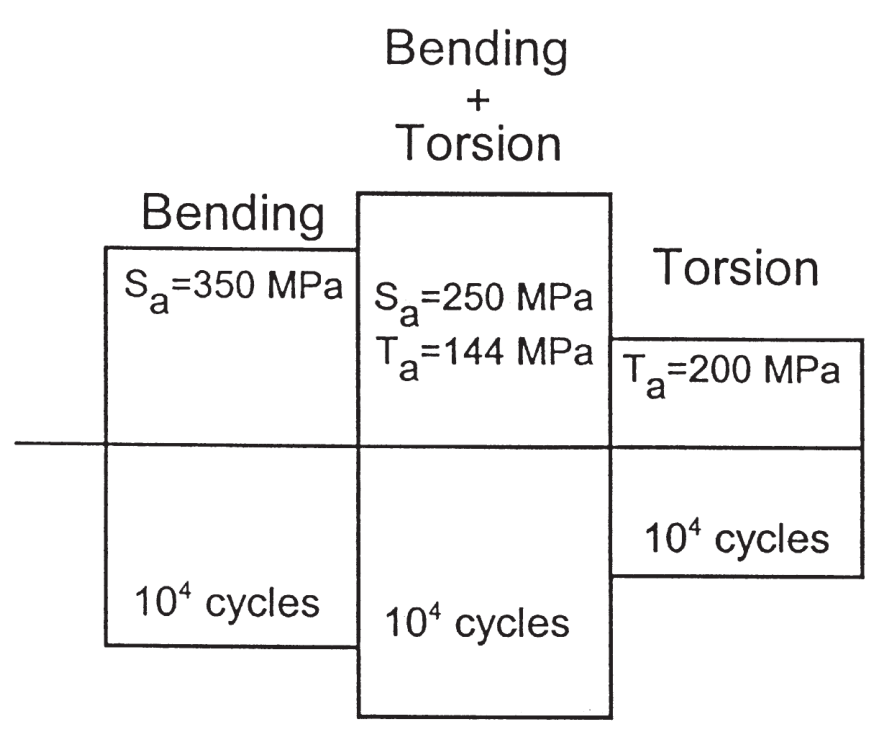
\includegraphics[width=0.6\textwidth]{figures//block.png} 
	\caption{block sequence tests (bending/bending+torsion/torsion) performed on a mild
		steel XC18.}
	\label{block}
\end{figure} 

Let us consider now a block sequence composed of
$10^4$ cycles of bending ($\Sigma_a =350 MPa$) followed by $10^4$
cycles of combined in-phase bending–torsion ($\Sigma_a ,T_a =250 MPa, 144 MPa$)
followed by $10^4$ cycles of torsion ($T_a =200 MPa$). This
sequence is repeated until the initiation of a crack. The
mean lifetime is found to be $N=1.73×10^5$ .

The three generalized fatigue
limits relative to the three blocks are estimated according
to Eq.\eqref{taus}:

$$\tau_{lim}^{bending}=155 MPa$$   $$\tau_{lim}^{torsion}=179 MPa$$  $$\tau_{lim}^{bend+tors}=157 MPa$$


These three values and the parameter $q$ are enough to
accumulate the damage in the three blocks using Eq.\eqref{NFsimple}:


$$\frac{\Gamma^{(bending)}}{\Gamma_R^{(bending)}}+\frac{\Gamma^{(bend+tors)}}{\Gamma_R^{(bend+tors)}}+\frac{\Gamma^{(torsion)}}{\Gamma_R^{(torsion)}}=1$$

The corresponding number of cycles to initiation is:
$N_{prediction} <1.5×10^5$ , that is to say five successive applications of the sequence. This prediction, close to the experimental result $N=1.73×10^5$ , is a conservative one.

It is important to note that if only one critical plane
(either from bending, torsion or bending+torsion
loading) is used for damage accumulation, one-third of
the damage would be calculated, resulting in a nonconservative prediction.

Morel's method is promising in its description aspect of limited endurance fatigue phenomenon, through the choice of the  mesoscopic plastic deformation. By using cumulative plasticity, a fatigue mechanisms occurring at the mesoscopic scale takes into account the main factors affecting the lifetime cycle fatigue (hydrostatic pressure and influence of phase shift). 

However, at the present stage, it does not completely meet the demand of a predictive tool. Indeed, it is a relatively complicated method (search critical plane $\Delta_c$ and accumulated damage in each direction in the plan); its application for multiaxial variable amplitude fatigue loads application data that are still not available (an S-N curve, two endurance limits and a particular  damage accumulation test). In addition, it is limited to soft materials. On the other hand, it is not completely free of counting method because its author uses the counting of the extrema of the evolution to get the macroscopic resolved shear stress $T(t)$ and the corresponding amplitude $P_a$ and mean values $P_m$ of the hydrostatic stress in each direction (m) in $\Delta_c$. With one purpose of calculating the limit of mesoscopic elasticity $\tau_lim$ in the saturation phase of the crystal. Again, this makes it difficult and daunting task.


\section{Space gradient effects}

The objective of the work is first to extend some classic high cycle fatigue (HCF) criteria (as Crossland, Dang Van, Papadopoulos, ...) in order  to take into account a sensitivity of the criteria to stress spatial variations occurring at length scale $l_g$, and second to compare the performances of the extensions through several experimental fatigue tests. After an introduction of the basic criteria and their gradient based extensions proposed by Luu et al., we focus on the Crossland criterion and we  propose a more practical and simple expression taking into account the gradient of the stress amplitude and the maximum hydrostatic stress.The generalization of the approach to other multiaxial fatigue criteria is also proposed.  The proposition is then tested and applied to different simple situations such as 4-point bending and cantilever rotative bending.  The relative errors between the exact solutions and the experimental data are estimated. Biaxial  bending-torsion tests are also simulated to demonstrate the capabilities of the approach.  In this work only stress gradient with a beneficial effect on fatigue have been considered. %An application to an industrial structure is finally performed.


\subsection{Introduction}

In several industries, the required design lifetime of many components often exceeds $ 10^8 $ cycles. This requirement is applicable to aircraft (gas turbine disks $ 10^{10} $ cycles), automobiles (car engine $ 10^8 $ cycles), and railways (high speed train $ 10^9 $ cycles). Although a large amount of fatigue data has been published in the form of S-N (where S is stress and N  the number of cycles to fatigue) curves, the data in the literature have been usually limited to fatigue lives up to $ 10^7 $ cycles. Using traditional fatigue criteria, a near hyperbolic relationship between stress and fatigue life is assumed, with an asymptotic limit defined as the fatigue limit (or endurance stress). 
A large number of multiaxial fatigue criteria, generalizing this notion of fatigue limit, are available in the literature \cite{Papadopoulos1997219}\cite{ballard1995high}\cite{suresh1998fatigue}. They are  used to design industrial components against failure. Nevertheless, most of these criteria present some drawbacks,  for instance when dealing with out-of-phase loading or with metals of different kinds from those used to develop the criteria. In fact, most of them are not designed to cope with high stress gradients such as those introduced  by surface treatments or notches, or to handle  scale effects as  specially present in nano or micro components. 

More precisely, as mentioned by Luu et al. \cite{luu2013formulation}, in problems related to small electronic components and electro-mechanical devices, at sufficiently small sizes, factors as size, gradient and loading effects affecting fatigue limits are not captured by classical fatigue criteria. In particular,  for the same in-state stress distribution as well as nominal maximum stress and material, the smaller the sample size is, the smaller the surface or the volume of the most stressed zone is, the higher the fatigue limit is.  Moreover, the nominal fatigue limit increases in the presence of stress gradient corresponding to a decreasing stress from the surface. Experimental example illustrates and makes clearer "beneficial gradient effect" \cite{Papadopoulos1996513}. The results of the constant moment tests on specimens of the same radius but different lengths shows that the gradient effect is an order of magnitude higher than the pure size effect. In this case, size effect is proved insignificant compared to the gradient effect at the considered scale.

From above it is concluded that the stress gradient factor is the most important contributer to this phenomenon. Fatigue criteria have been  generalized by several authors by including a  gradient dependence \cite{Papadopoulos1996513} in order to  introduce a sensitivity of the endurance limit to space variations occurring at length scale  $l_g$. Uniaxial normal cyclic stress states with non-zero and zero normal stress gradients, respectively,give some indication about the normal stress gradient effect. The larger the normal stress due to bending, the larger the difference between bending test points and tension-compression ellipse arc (as is shown in \figref{fig2}).
\begin{figure}[!h]
	\centering
	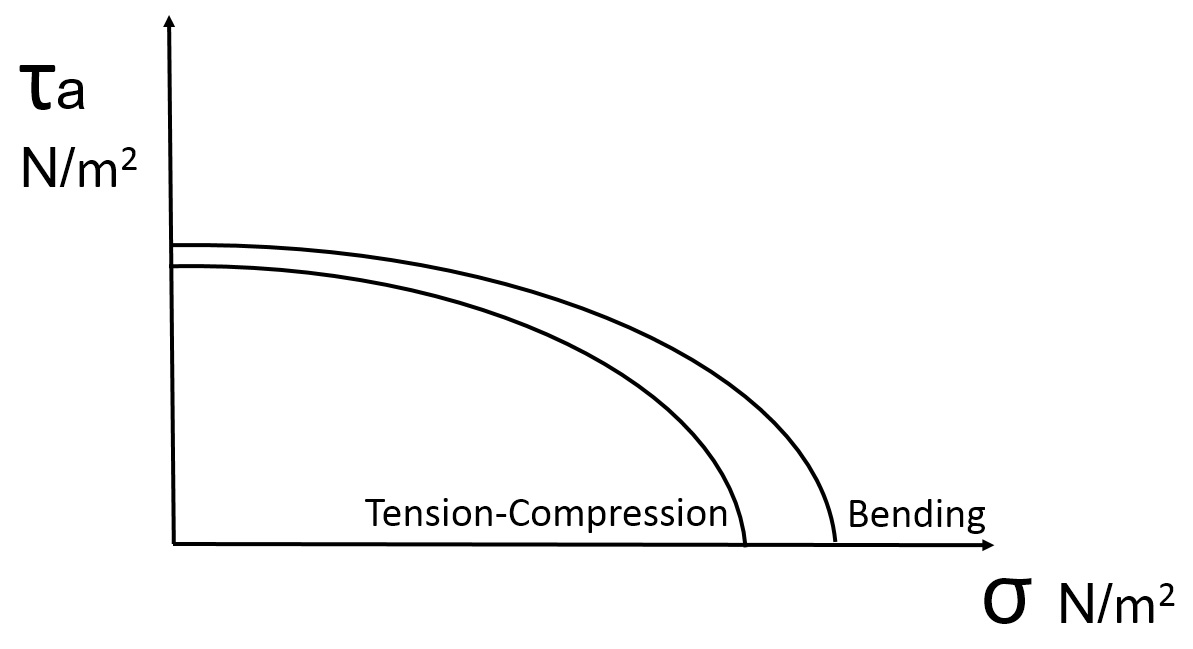
\includegraphics[width=0.8\textwidth]{figures//fig2.jpg} 
	\caption{Schematic representation of the nominal fatigue limit (ellipse arc) for two different tests: the arc is larger in the case of bending-torsion (presence of stress gradient) than in tension-compression.}
	\label{fig2}
\end{figure}

Apart from gradient approaches\cite{Amargier20101904}\cite{Papadopoulos1996513}, to take account of these effect, others approaches such critical volume \cite{maitournam2009fatigue}, critical distance\cite{taylor2010theory}\cite{Araujo200795}, critical layer\cite{flavenot1983epaisseur}, averaging over a specific volume \cite{palin2000stress}\cite{Banvillet2003755} are used . In fact, all the approaches are equivalent to introducing a length scale. 
In the paper, we consider specifically the gradient approach. We start from the proposition of Luu et al., and propose and a simpler way to account for the gradient. The Crossland criterion, one of the most widely known HCF criteria, is used to illustrate the approach. Crossland proposed that the second invariant of the deviatoric stress tensor and the hydrostatic stress are the variables governing the endurance limit. 
The new proposition adds two gradient terms ; it is then calibrated and its predictions are compared to experimental results to check its relevancy.


\subsection{A first gradient approach \cite{luu2013formulation}}
\subsubsection{General formulation}

Luu et al. \cite{luu2013formulation} proposed extensions of classical HCF fatigue criteria using the gradients of the shear and normal stress to account for the gradient effect. In the case of critical plane type criteria, they defined a generalized shear stress amplitude including shear stress gradient and a generalized maximum normal (or hydrostatic) stress.
A general form of classical fatigue limit criteria can be written as follows:
\begin{equation}
\label{eq:classical}
f(C_a(n^*),N_{max}(n^*))=C_a(n^*)+aN_{max}(n^*)-b\geqslant 0 ,
\end{equation}
with a, b being two material parameters. $f$ is a function, chosen in many cases as linear, and $n^*$ is the normal vector of the critical plane; $C_a(n^* )$, $N_{max} (n^* )$ are respectively the amplitude of shear stress and the maximum value of the normal stress on the critical plane.

A new class of fatigue criteria extended from classical ones with stress gradient terms introducing not only in the normal stress but also in the shear stress components, was proposed. It concerns only free defect materials and can model both phenomena ``smaller is Stronger and Higher Gradient is Stronger". 

Besides the stress gradient term appearing in the normal stress part in form of $G=\Delta(\sigma_{11}+\sigma_{22}+\sigma_{33})$, another gradient term, the gradient of the stress tensor amplitude (or alternatively of deviatoric stress tensor amplitude) $\parallel{Y}_a\parallel={\Delta\sigma}_a$ is added to the shear stress amplitude part. Basing on all these analyses a new form of fatigue criteria taking into account gradient effects, is proposed:
\begin{equation}
f(\widetilde{C_a}(n^*),\widetilde{N_{max}}(n^*))=\widetilde{C_a}(n^*)+a\widetilde{N}_{max}(n^*)-b\geqslant 0 ,
\label{eq:gradient crossland}
\end{equation}
where $\widetilde{C_a}(n^*)$ and $\widetilde{N_{max}}(n^*)$ are extended definitions of the amplitude of shear stress and of the normal stress taking into account the presence of local gradient.

In the following we first focus on the Crossland criterion and its extension.

\subsubsection{Recall of the classical Crossland criterion}

The classical Crossland criterion defines the fatigue limit of metallic specimens subjected to multi-axial cyclic stress\cite{Crossland} by : 
\begin{equation}
f(\sqrt{J_{2,a}},\sigma_{H,max})=\sqrt{J_{2,a}}+a\sigma_{H,max}-b\leqslant 0\label{eq:crossland}
\end{equation}
where $\sqrt{J_{2,a}}$ measures  the amplitude of variation of the second invariant of the deviatoric stress  and $\sigma_{H,max}$ is the maximum hydrostatic stress observed during a loading cycle. The parameters $a$ and $b$ are material constants to be calibrated experimentally. The amplitude of the square root of the second invariant of the stress deviator can be defined, in general case, as the half-length of the longest chord of the deviatoric stress path or as the radius of the smallest hypersphere circumscribing the stress deviator loading path \cite{Papadopoulos1997219}
\begin{equation}\sqrt{J_{2,a}}=\dfrac{1}{2\sqrt{2}}\min \limits_{\uline{\uline{S_1}}}\left\lbrace \max \limits_{t}\sqrt{(\uuline{S}(t)-\uuline{S_1}):(\uuline{S}(t)-\uuline{S_1})}\right\rbrace . \end{equation}

The deviatoric stress $\uuline{S}$ associated with a stress tensor $\uuline{\sigma}$  is defined by
\begin{equation} \uuline{S}=\uuline{\sigma}-\dfrac{1}{3}\textrm{tr}\uuline{\sigma}\, \uuline{I}
\end{equation}
where $\textrm{tr}\uuline{\sigma}$ is the trace of the stress tensor $\uuline{\sigma}$ and $\uuline{I}$ the second order unit tensor.

The maximum value that the hydrostatic stress reaches during the loading cycle is on the other hand:
\begin{equation}
\sigma_{H,max}=\max\limits_{t}\left\lbrace \dfrac{1}{3}\textrm{tr}(\uuline{\sigma}(t))\right\rbrace .
\end{equation}

For a proportional cyclic loading, if one introduces the two extreme stress tensors $\uuline{\sigma}^A$ and $\uuline{\sigma}^B$ observed during the loading path, together with the stress range 
\begin{equation}\Delta\uuline{\sigma}=\uuline{\sigma}^B-\uuline{\sigma}^A\end{equation}
and its deviatoric part $\uuline{\Delta s} $, the variation of
the second invariant of the stress deviator reduces to 
\begin{equation}\sqrt{J_{2,a}}=\dfrac{1}{2}\max\limits_{t}\sqrt{\dfrac{1}{2}\Delta\uuline{s}:\Delta\uuline{ s}}=\dfrac{1}{2}\max\limits_{t}\sqrt{\dfrac{1}{2}\left( \Delta s_{11}^2+\Delta s_{22}^2+\Delta s_{33}^2+2\Delta s_{12}^2+2\Delta s_{13}^2+2\Delta s_{23}^2\right) }.\end{equation}


The material constants $a$ and $b$ can be related to  the limit $t_{-1}$ of endurance in alternate torsion and to the limit $s_{-1}$ of endurance in alternate tension-compression by
\begin{equation}
a=\dfrac{3 t_{-1}}{s_{-1}}-\sqrt{3},\quad 
b=t_{-1}.
\label{crossland-ab}
\end{equation}

\subsubsection{Formulation of Crossland criterion with gradient effect}

In particular, using as a basis the classical Crossland criterion Eq.\eqref{eq:crossland} and the general framework for the development of a gradient dependent fatigue limit criterion Eq.\eqref{eq:gradient crossland}, a new version can be written in the form:
\begin{equation}
\sqrt{\widetilde{J_{2,a}}}+a\widetilde{\sigma_{H,max}}\leqslant b .
\end{equation}

This formula takes into account the indicator of the influence of the gradient of the stress deviator which reflects the spatial non-uniform distribution of stress state.

In practice, \cite{luu2013formulation} had proposed:
\begin{equation}
\sqrt{{J_{2,a}}}\sqrt{1-\left(l_\tau\dfrac{\parallel \uuline{\uline{Y}}\parallel_{,a}}{\parallel \uuline{S}\parallel_{,a}}\right)^{n_\tau}}+a\sigma_{H,max}\left(1-\left\langle  l_\sigma\dfrac{\parallel G\parallel}{\sigma_{H,max}}\right\rangle ^{n_\sigma}\right)-b < 0 .
\end{equation}

Here $\parallel \uuline{\uline{Y}}\parallel_{,a}$ is the full stress gradient and $\parallel G\parallel$ is used as an indicator of the influence of the normal stresses gradient.

\begin{equation}
\parallel{G}\parallel=\parallel{\nabla \sigma_{H,max}}\parallel=\sqrt{\left(\dfrac{\partial \sigma_{H,max}}{\partial x}\right)^2+\left(\dfrac{\partial \sigma_{H,max}}{\partial y}\right)^2+\left(\dfrac{\partial \sigma_{H,max}}{\partial z}\right)^2} .
\end{equation}



\subsection{Optimized Crossland Criterion formulation}
The precedent Luu and al. formula has six materials parameters $a$,$b$,$l_\tau$,$l_\sigma$,$n_\tau$,$n_\sigma$ to be identified experimentally. The calibration can be complicated ; it does not lead to a unique set of parameters. Physical considerations, such as the length scales, have to be taken into account for choosing the optimized material constants. For practical application in an industrial context, it is essential to reduce the number of parameters. We therefore wish to investigate a simpler construction, departing from the classical Crossland criterion.

Surfaces with stresses decreasing in depth are, here and after, considered. Failure occurs at the point $x_0$ when,  $(\sqrt{J_{2,a}}+a\sigma_{H,max}-b)(x_0)\geqslant 0 $. To be more general and avoid singularity, this condition should be satisfied in some $x_0$ neighboring volume of size $l_g$, leading to a criterion given by:

\begin{equation}
\inf\limits_{\uline{x}\in B\left( \uline{x_0},\,\uline{l_g}\right) }\left( \sqrt{J_{2,a}}+a\sigma_{H,max}-b\right) (x)\geqslant 0 .
\label{crossland-x0-2}
\end{equation}

To obtain a suitable expression, an expansion of Eq.(\ref{crossland-x0-2}) in performed in the neighborhood of ${x_0}$. The sought formula should account for the beneficial effect of the stress gradient. Considering that the stress is decreasing in depth, a negative sign is associated with the norm of the gradient of stress tensor in to the proposed formula. In addition, the gradient term should not only affect hydrostatic stress but also shear stress.

An objective formulation based on the lowest possible value of $\sqrt{J_{2,a}}$ and of $\sigma_{H,max}$ in the neighborhood, is finally:

\begin{equation}
\sqrt{J_{2,a}}+a\sigma_{H,max}-l_g\parallel{\nabla\sqrt{J_{2,a}}}+a\nabla{\sigma_{H,max}}\parallel\leqslant b ,
\label{modified Crossland}
\end{equation}
We keep the same material parameters $a$ and $b$ as before. $l_g$ is a characteristic length to be optimized to match the experimental results. The approach has only one supplementary material constant whose calibration is easy.

\subsection{Optimized Papadopoulos Criterion formulation}
Papadopoulos\cite{papadopoulos1993fatigue} proposes to opt for a mean value of the accumulated plastic strain on all possible slip systems of representative elementary volume(REV). So he chose to use a average value  of accumulated plastic deformation rather than looking at failure of a single crystal. A spherical coordinate system(\figref{fig50}) to guide the vector of normal in material plane, and the unit orientation vector $r$ linked to a sliding direction of this plan is used to conduct the integration over all possible orientations.

\begin{figure}[h!]
	\centering
	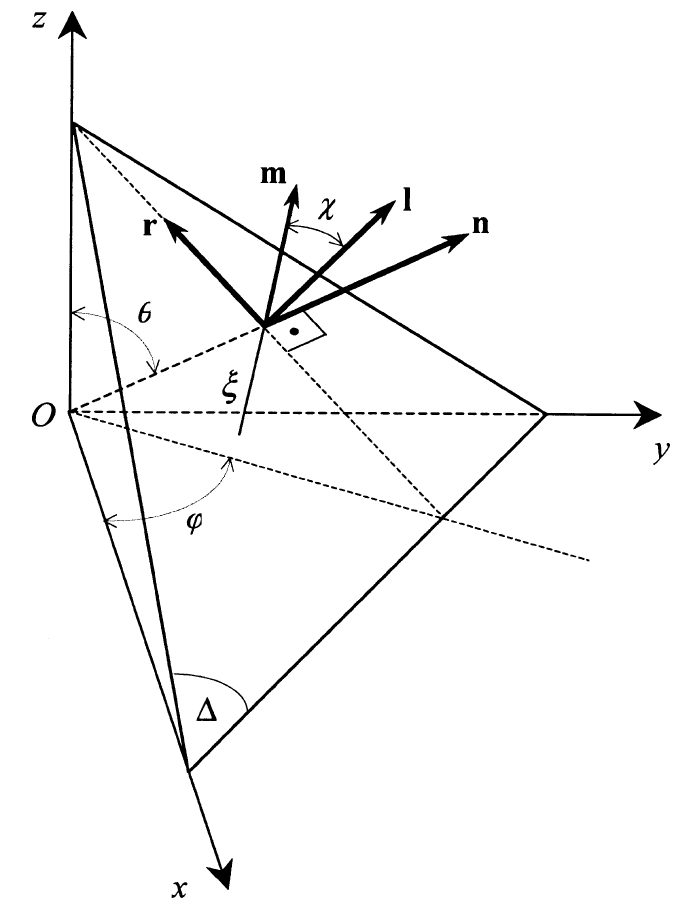
\includegraphics[width=0.5\textwidth]{figures//demopp.png} 
	\caption{Material plane $\Delta$ passing through point O of a body and its
		associated (n, l, r) frame.}
	\label{fig50}
\end{figure}
At any point $O$ of a body, a material plane $\Delta$ can be defined by its unit normal vector $\bf n$. This vector
$\bf n$ makes an angle $\theta$ with the z-axis of a $Oxyz$ frame attached to the body, and its projection on the $xy$ plane
makes an angle $\varphi$ with axis $x$. For each plane $\Delta$ a new quantity is introduced as the quadratic mean value, over all the sliding directions of the considered plane, of the resolved shear stress amplitude and denoted as $T_a$.This shear stress quantity was first introduced in Papadopoulos [6]
and was subsequently used by other researchers.The critical plane according to our proposal is that onto which $T_a(\varphi,\theta)$ achieves its maximum value. The fatigue limit criterion is written as:
\begin{equation}
max T_a+\alpha_\infty \sigma_{h,max}\leqslant \gamma_\infty
\end{equation}
where $\alpha_\infty$ and $\gamma_\infty$ are material parameters to be determined\cite{papadopoulos2001long}.
$$\sigma_{h,max}=\max\limits_{t}\left\lbrace \dfrac{1}{3}tr(\uline{\uline{\sigma}}(t))\right\rbrace $$
The construction of $T_a$ is based on the calculation of a local shear stress $\tau$:
\begin{equation}
\begin{split}
\tau=&[sin\theta cos\varphi\sigma_{xx}+sin\theta sin\varphi\sigma_{xy}+cos\theta\sigma_{xz}](-sin\varphi cos\chi-cos\theta cos\varphi sin\chi)+\\&[sin\theta cos\varphi\sigma_{xy}+sin\theta sin\varphi\sigma_{yy}+cos\theta\sigma_{yz}](cos\varphi cos\chi-cos\theta sin\varphi sin\chi)+\\&[sin\theta cos\varphi\sigma_{xz}+sin\theta sin\varphi\sigma_{yz}+cos\theta\sigma_{zz}]sin\theta sin\chi
\end{split} 
\label{eqres}
\end{equation}
It is clear that this shear stress is a function of
$\varphi$, $\theta$, $\chi$ and of time $t$ in the case of variable loading, i.e. $\tau=\tau(\varphi, \theta, \chi, t)$. Upon fixing a pair of angles $(\varphi, \theta)$ (i.e. a plane
$\Delta$) and an angle $\chi$ (i.e. a line $\xi$ on $\Delta$), one can define the amplitude of the resolved shear stress $\tau_a$, acting on $\Delta$
along $\xi$ by the formula:
\begin{equation}
\tau_a(\varphi,\theta,\chi)=\dfrac{1}{2}\big[\max \limits_{t\in P}\tau_a(\varphi,\theta,\chi ,t)-\min \limits_{t\in P}\tau_a(\varphi,\theta,\chi ,t)\big]
\end{equation}
Now, for a given plane $\Delta$, i.e. for a fixed pair of angles ($\varphi$, $\theta$),
the generalized shear stress amplitude $T_a$ is defined as the $L^2$ average in the plane $\Delta$ of the amplitude of resolved shear stress:
\begin{equation}
T_a(\varphi,\theta)=2\sqrt{\dfrac{1}{\pi}\int_{x=0}^{\frac{\pi}{2}} \tau_a^2(\varphi,\theta,\chi)d\chi}
\label{Ta}
\end{equation}
We note the fatigue limit in fully reversed torsion $t_{-1}$ and the fatigue limit in fully reversed bending $f_{-1}$. From these two tests we get the parameters:
$$\gamma_\infty=t_{-1},$$ 
$$\alpha_\infty=3\left( \dfrac{t_{-1}}{f_{-1}}-\dfrac{1}{2}\right) .$$
The Papadopoulos fatigue limit criterion achieves the form:
\begin{equation}
maxT_a+3\left( t_{-1}/f_{-1}-1/2\right) \sigma_{h,max}\leqslant t_{-1}.
\label{eq:papadopoulos}
\end{equation}
Now,  the Papadopoulos Criterion can be simply extended  to cases with gradient effects by
\begin{equation}
maxT_a+\alpha_\infty\sigma_{H,max}-l_g\parallel\nabla{maxT_a}+\alpha_\infty\nabla\sigma_{H,max}\parallel\leqslant \gamma_\infty .
\label{eq:modified papa}
\end{equation}

\subsection{Optimized Dang Van Criterion formulation}
The Dang Van criterion as presented in \cite{ballard1995high} is expressed as:
\begin{equation}
\max \limits_{\vec{n}}\left\lbrace \max \limits_{t}\left\{\tau{(\vec{n},t)}+a_D\sigma_H(t)\right\}\right\rbrace \leqslant b_D.
\label{dv}
\end{equation}

Here, $\tau$ denotes the mesoscopic shear stress and is obtained from a mesoscopic stress tensor $\hat{\bm{\sigma}}$ defined by:
$$\hat{\bm{\sigma}}(t)=(\bm{\sigma}(t)-s^\star),$$
where $s^\star$ is the center of the smallest hypersphere circumscribed to the loading path in deviatoric stress space. It is obtained by solving a ``min-max" problem as follows:
$$s^\star = arg \min\limits_{s_1}\left\{\max\limits_t\parallel s(t)-s_1\parallel\right\}.$$
In the case of fully reversed loading, the values $s^\star=0$ can be directly deduced without solving the ``min-max problem" as in general case.

The principal stress values of stress tensor $\widetilde{\sigma}$ being denoted  by $\hat{\sigma}_{\Rmnum{3}}(t)\leqslant\hat{\sigma}_{\Rmnum{2}}(t)\leqslant\hat{\sigma}_{\Rmnum{1}}(t)$, one gets the amplitude of shear stress by:
$$\tau(t)=\dfrac{1}{2}\left( \hat{\sigma}_{\Rmnum{1}}(t)-\hat{\sigma}_{\Rmnum{3}}(t)\right) .$$
Moreover, $\sigma_H(t)$ denotes  the hydrostatic stress as a function of the time.
The material characteristic parameters $a_D$ and $b_D$ are finally  given from traction compression and torsion fatigue limites by  :
$$a_D=\dfrac{3t_{-1}}{s_{-1}}-\dfrac{3}{2};$$  $$b_D=t_{-1}.$$

Now,  the Dang Van criterion can be extended to a graident dependent criterion by 
\begin{equation}
\max \limits_{t}\left\{\tau{(t)}+a_D\sigma_H(t)\right\}-l_g\parallel	\max \limits_{t}\left\{{\nabla\tau{(t)}}+a_D\nabla\sigma_H(t)\right\}\parallel\leqslant b_D.
\label{modified dangvan}
\end{equation}
\subsection{Calibration of the critera}

In this section, two different uniaxial fatigue tests with stress gradient effects are used to calibrate the optimized gradient Crossland, Papadopoulos and DangVan criteria. An application to a biaxial test fatigue test shows the ability of the proposed approach to account for stress gradient in multiaxial cases. 


\subsubsection{Fully reversed 4-point bending and rotating cantilever bending fatigue tests}
\textbf{With Crossland criterion}
The model of 4-point bending is first considered. The bar made of steel has both ends fixed. The radius $R$ is a variable ranging from 1mm to 30mm in order to  challenge the fact "the smaller, the stronger". The length $L$ of the bar is 100 mm.

\begin{figure}[h!]
	\centering
	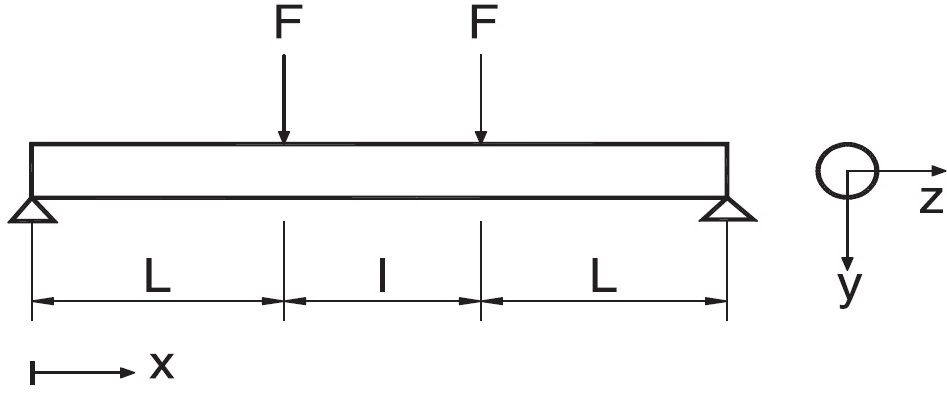
\includegraphics[width=0.4\textwidth]{figures//fig11.jpg} 
	\caption{4-point bending test \cite{Papadopoulos1996513} }
	\label{fig11}
\end{figure}

The bending moment is the same in the interval $L\leqslant x \leqslant L+l$ and equal to
$M = FL$ (\figref{fig11}).
For $L\leqslant x \leqslant L+l$ and  $-R\leqslant y \leqslant R$, the bending stress $\bm{\sigma}$  is
\begin{equation}
\uuline{\sigma}=\sigma_{xx}sin(wt)e_x\otimes e_x=\dfrac{FLy}{I}sin(wt) e_x\otimes e_x \label{bending4} \end{equation}
with $I=\pi R^4/4$.  The maximum stress during the cyclic loading in the bar  is thus 
$ \sigma_{max}=\dfrac{FLy}{I}$, 
while the macroscopic stress range is $ \Delta\uuline{\sigma}(t)=2\sigma_{max}e_x\otimes e_x $, and the 
hydrostatics stress takes the value
\begin{equation}
\sigma_{H,max}=\max\limits_{t}\left\lbrace \dfrac{1}{3}\textrm{tr}(\sigma(t))\right\rbrace =\dfrac{1}{3}\sigma_{max}=\dfrac{FLy}{3I}.
\end{equation}
From the value of  the deviatoric stress
\begin{equation} 
\Delta\uuline{ S}=\Delta\uuline{\sigma}-\dfrac{1}{3}\textrm{tr}\Delta\uuline{\sigma}\uuline{I}=
\left(
\begin{array}{ccc}
\dfrac{4}{3}\sigma_{max} & 0 & 0\\
0 & -\dfrac{2}{3}\sigma_{max} & 0\\ 
0 & 0 & -\dfrac{2}{3}\sigma_{max}\\
\end{array}\right) ,
\end{equation}
we can compute the second invariant of the stress deviator :
\begin{equation}
\sqrt{J_{2,a}}=\dfrac{1}{2\sqrt{2}}\sqrt{\Delta \uuline{S}:\Delta \uuline{S}}=\dfrac{\sigma_{max}}{\sqrt{3}} =\dfrac{FLy}{\sqrt{3}I} .
\end{equation}


Then the gradient part is given by:
\begin{equation}
\nabla\sqrt{J_{2,a}}=\dfrac{\partial\sqrt{J_{2,a}}}{\partial x}\uline{e}_x+\dfrac{\partial\sqrt{J_{2,a}}}{\partial y}\uline{e}_y+\dfrac{\partial\sqrt{J_{2,a}}}{\partial z}\uline{e}_z=\left( 0,\dfrac{FL}{\sqrt{3}I},0\right)  ,
\end{equation}
and
\begin{equation}
\nabla \sigma_{H,max}=(0,\dfrac{FL}{3I},0).
\end{equation}
The parameters $a$ and $b$ of the standard Crossland criterion, are obtained from fully reversed tension-compression fatigue limit $s_{-1}$  and torsion fatigue limit $t_{-1}$ using Eq.(\ref{crossland-ab}).

From Eq.(\ref{eq:crossland}), standard Crossland criterion without gradient effect (for radius $R$) is:
\begin{equation}
\sqrt{J_{2,a}}+a\sigma_{H,max}=\dfrac{FLR}{\sqrt{3}I} +\dfrac{aFLR}{3I}\leqslant b.
\label{eq4pcross}
\end{equation}
The gradient term here is given by:
\begin{equation}
\parallel{\nabla\sqrt{J_{2,a}}}+a{\nabla \sigma_{H,max}}\parallel=\dfrac{FL}{\sqrt{3}I}+\dfrac{aFL}{3I}.
\label{cross-gradient-term}
\end{equation}

By comparison we can see in 4-point bending test the difference between classical and modified Crossland criterion corresponds to the product of the characteristic length $l_g$ by the term (\ref{cross-gradient-term}) associated to the decrease of the stress in depth. This value shows how much the modification affects the Crossland criterion. 

\noindent Crossland criterion with beneficial gradient term as shown in Eq.(\ref{modified Crossland}) is given by:
\begin{equation}
\begin{split}
\sqrt{J_{2,a}}+a\sigma_{H,max}-l_g(\parallel{\nabla\sqrt{J_{2,a}}}+a\nabla{\sigma_{H,max}}\parallel)&=\\ \dfrac{FLR}{\sqrt{3}I} +\dfrac{aFLR}{3I}-l_g\left( \dfrac{FL}{\sqrt{3}I}+\dfrac{aFL}{3I}\right) 
&=\\ \dfrac{1}{\sqrt{3}}\sigma_{max}+\dfrac{a}{3}\sigma_{max}-l_g\left( \dfrac{1}{\sqrt{3}R}\sigma_{max}+\dfrac{a}{3R}\sigma_{max}\right) &\leqslant b\, ,
\end{split}
\end{equation}
which is to say:
\begin{equation}
\sigma_{max}\leqslant\dfrac{b}{\dfrac{1}{\sqrt{3}}+\dfrac{a}{3}-l_g\left( \dfrac{1}{\sqrt{3}R}+\dfrac{a}{3R}\right) }\, .
\end{equation}

The material parameters $a$ and $b$ are obtained using their classical expressions as Eq.(\ref{crossland-ab}) from tests free of stress gradient. The corresponding fatigue limit are denoted $s_{ref}$ for the alternate tension-compression test, and $t_{ref}= b$ for the alternate torsion test. For a specimen of radius $R$
the alternate bending fatigue limit is denoted $f_c(R)$.
We can observe that:
\begin{equation}
f_c(R)=\dfrac{b}{\dfrac{1}{\sqrt{3}}+\dfrac{a}{3}-l_g\left( \dfrac{1}{\sqrt{3}R}+\dfrac{a}{3R}\right) }\geqslant s_{ref} = \dfrac{b}{\dfrac{1}{\sqrt{3}}+\dfrac{a}{3}},
\label{crossland-fr}
\end{equation}
and that $f_c(R)$ tends to $s_{ref}$ for large values of $R$.

\textbf{With Papadopoulos criterion}  
From \ref{bending4}, the resolved shear stress $\tau$ acting along a line $\xi$ of a plane $\Delta$ is given by Eq.\ref{eqres}, which in this case leads to:
\begin{equation}
\tau(\varphi,\theta,\chi,t)=\sigma_{xx}sin(2\pi t/P)sin\theta cos\theta sin\chi.
\end{equation}
Clearly, for the worse case in $\chi$,  the resolved shear stress amplitude is equal to:
\begin{equation}
\tau_a(\varphi,\theta,\chi)=\sigma_{xx}|sin\theta cos\theta sin\chi|.
\end{equation}
The generalized shear stress amplitude $T_a$ becomes:
\begin{equation}
T_a(\varphi,\theta)=2\sqrt{\dfrac{1}{\pi}\int_{\chi=0}^{\frac{\pi}{2}}(\sigma_{xx}|sin\theta cos\theta sin\chi|)^2d\chi}
\end{equation}
The maximum value of $T_a$ is obtained at ($\theta=\pi/4$) and at ($\theta=3\pi/4$). It is equal to:
\begin{equation}
maxT_a=\sigma_{xx}/2
\end{equation}
The hydrostatic stress is given by:
\begin{equation}
\sigma_{H}(t)=\dfrac{1}{3}\sigma_{xx}sin(2\pi t/P)
\end{equation}
The maximum value of $\sigma_H$ reached in a loading cycle is:
\begin{equation}
\sigma_{H,max}=\sigma_{xx}/3
\end{equation}
Papadopoulos criterion with beneficial gradient term as shown in Eq.\eqref{eq:modified papa} is then given by:
\begin{equation}
\begin{split}
maxT_a+\alpha_\infty\sigma_{H,max}-l_g\parallel\nabla{maxT_a}+\alpha_\infty\sigma_{H,max}\parallel&=\\\dfrac{FLR}{2I} +\dfrac{\alpha_\infty FLR}{3I}-l_g\left( \dfrac{FL}{2I}+\dfrac{\alpha_\infty FL}{3I}\right) &=\\ \dfrac{1}{2}\sigma_{max}+\dfrac{a}{3}\sigma_{max}-l_g\left( \dfrac{1}{2R}\sigma_{max}+\dfrac{a}{3R}\sigma_{max}\right) &\leqslant \gamma_\infty = t_{ref} ,
\end{split}
\end{equation}
which is to say:
\begin{equation}
\sigma_{max}\leqslant\dfrac{\gamma_\infty}{\dfrac{1}{2}+\dfrac{\alpha_\infty}{3}-l_g(\dfrac{1}{2R}+\dfrac{\alpha_\infty}{3R})} .
\end{equation}
For a specimen of radius $R$
the alternate bending fatigue limit is denoted $f_p(R)$.
We can observe that:
\begin{equation}
f_p(R)=\dfrac{\gamma_\infty}{\dfrac{1}{2}+\dfrac{\alpha_\infty}{3}-l_g\left( \dfrac{1}{2R}+\dfrac{\alpha_\infty}{3R}\right) }\geqslant s_{ref} = \dfrac{\gamma_\infty}{\dfrac{1}{2}+\dfrac{\alpha_\infty}{3}}.
\label{papa-fr}
\end{equation}

\textbf{With Dang Van criterion}  
Under fully reversed loading we have:
$$\tau(t)=\dfrac{1}{2}(\sigma_{xx}(t)-0)$$ 
From Eq.\eqref{modified dangvan} we can deduce Dang Van criterion.
\begin{equation}
\begin{split}
\max \limits_{t}\left\{\tau{(t)}+a_D\sigma_H(t)\right\}-l_g\parallel{\nabla\tau{(t)}}+a_D\nabla\sigma_H(t)\parallel&=\\ \dfrac{FLR}{2I} +\dfrac{aFLR}{3I}-l_g\left( \dfrac{FL}{2I}+\dfrac{aFL}{3I}\right) &=\\ \dfrac{1}{2}\sigma_{max}+\dfrac{a}{3}\sigma_{max}-l_g\left( \dfrac{1}{2R}\sigma_{max}+\dfrac{a}{3R}\sigma_{max}\right) &\leqslant b_D= t_{ref}\, ,
\end{split}
\end{equation}
which is to say:
\begin{equation}
\sigma_{max}\leqslant\dfrac{b}{\dfrac{1}{2}+\dfrac{a}{3}-l_g\left( \dfrac{1}{2R}+\dfrac{a}{3R}\right) }.
\end{equation}
We can observe that the corresponding bending limit is thus
$$f_D(R)=\dfrac{b}{\dfrac{1}{2}+\dfrac{a}{3}-l_g\left( \dfrac{1}{2R}+\dfrac{a}{3R}\right) }\geqslant s_{ref} = \dfrac{b}{\dfrac{1}{2}+\dfrac{a}{3}}.
$$


\textbf{Comparison with experimental data}
\begin{figure}[!h]
	\begin{center}
		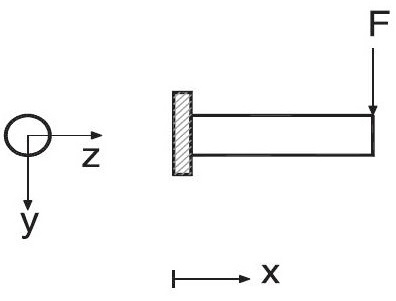
\includegraphics[width=0.5\textwidth]{figures//fig3.jpg} 
		\caption{Cantilever bending test \cite{papadopoulos1996invariant}}
		\label{fig9}
	\end{center}
\end{figure}
The case of cantilever fully reversed bending corresponds to the four point bending test except that there, the bending moment is function of $x$. Thus, the maximum stress $\sigma_{max}$ for a given section is a function of $x$. But, the $y$ dimension of the beam is much smaller than its $x$ dimension, which allows us to neglect gradients in $x$ . All  expressions of the four point bending case thus  apply to this cas. 

\newpage
\begin{Figure}[h!]{Fatigue limits with gradient effect for different radii.}[label]
	\graphfile*[34]{figures//carbonsteel.png}[]
	\graphfile*[34]{figures//1220steel.png}[]
	\\
	\graphfile*[34]{figures//1035steel.png}[]
	\graphfile*[34]{figures//40khsteel.png}[]
\end{Figure}

Eq.(\ref{crossland-fr}) with $a$ et $b$ calibrated from given $S_{ref}$ and $t_{ref}$ is used to estimate the characteristic length $l_g$ in order to give the best correlation between simulated and experimental fatigue limit obtained in rotating cantilever bending tests for different materials and radii. The results are sketched in Fig.(\ref{label}) and the corresponding parameters are shown in Table.\ref{tab.paras}.

\begin{table}[!h]
	\centering
	\caption{Length scales of different materials}
	\label{my-label}
	\begin{tabular}{crrrr}
		\hline
		\textbf{}                                                                   & \multicolumn{1}{c}{\textbf{1220 steel}} & \multicolumn{1}{c}{\textbf{Carbon steel}} & \multicolumn{1}{c}{\textbf{1035 steel}} & \multicolumn{1}{c}{\textbf{40Kh steel}} \\ \hline
		\textbf{\begin{tabular}[c]{@{}c@{}}$\bm{S_{ref}}$\\ {[}MPa{]}\end{tabular}} & 191                                     & 222                                       & 234                                     & 297                                     \\
		\textbf{\begin{tabular}[c]{@{}c@{}}$\bm{t_{ref}}$\\ {[}MPa{]}\end{tabular}} & 143                                     & 151                                       & 172                                     & 180                                     \\
		\textbf{\begin{tabular}[c]{@{}c@{}}$\bm{l_g}$\\ {[}mm{]}\end{tabular}}      & 0.3755                                  & 0.3297                                    & 0.2861                                  & 0.1424                                  \\ \hline
	\end{tabular}
	\label{tab.paras}
\end{table}

We can observe a very interesting phenomenon that the smaller fatigue limit is, the larger influence of gradient effect is.


\subsubsection{Bending-torsion fatigue tests}
\textbf{With Crossland criterion}
The bending moment is a linear function of $x, M_b= -F(L-x)$. The twisting moment is denoted $M_t$. The stress $\sigma_{xx}$ now varies along the depth (i.e. y-axis) and the length (i.e. x-axis) of the specimen, but as above we will neglect the gradient in $x$ as compared to the gradient in $y$. The bending stress is given here by : 
\begin{equation}
\sigma_{a}=\dfrac{-F(L-x)}{I}R=\dfrac{M_b}{I}y \quad \text{ with } \quad I=\dfrac{\pi R^4}{4},
\end{equation}
while the twisting shear stress is given by 
$ \tau_{a}=\dfrac{M_t}{J}y \quad \text{ with  }
J=\dfrac{\pi R^4}{2}$. 
The stress tensor $\uuline{\sigma}$ is then:
\begin{equation} 
\uline{\uline{\sigma}}(t)=
\left(
\begin{array}{ccc}
\sigma_{a}sin(\omega t) & \tau_asin(\omega t) & 0\\
\tau_asin(\omega t) & 0 & 0\\ 
0 & 0 & 0\\
\end{array}\right) .
\end{equation}
Its range tensor is:
\begin{equation} 
\Delta\uuline{\sigma}=
\left(
\begin{array}{ccc}
2\sigma_a& 2\tau_a & 0\\
2\tau_a& 0 & 0\\ 
0 & 0 & 0\\
\end{array}\right) ,
\end{equation}
with deviator
\begin{equation} 
\Delta\uuline{ S}=\Delta\uuline{\sigma}-\dfrac{1}{3}\textrm{tr}\Delta\uuline{\sigma}=
\left(
\begin{array}{ccc}
\dfrac{4}{3}\sigma_{a} & 2\tau_a & 0\\
2\tau_a & -\dfrac{2}{3}\sigma_a & 0\\ 
0 & 0 & -\dfrac{2}{3}\sigma_a\\
\end{array}\right) .
\end{equation}
The second invariant of the stress deviator is then:
\begin{equation}
\sqrt{J_{2,a}}=\dfrac{1}{2\sqrt{2}}\sqrt{\Delta \uuline{S}:\Delta \uuline{S}}=\sqrt{\dfrac{1}{3}\sigma_a^2+\tau_a^2}=\sqrt{\dfrac{M_b^2}{3I^2}+\dfrac{M_t^2}{J^2}}y.
\end{equation}
As for the  hydrostatics stress, we have
\begin{equation}
\sigma_{H,max}=\max\limits_{t}\left\lbrace \dfrac{1}{3}\textrm{tr}(\sigma(t))\right\rbrace =\dfrac{\sigma_{a}}{3}=\dfrac{M_b}{3I}y .
\end{equation}
Then the gradient part has the value:
\begin{equation}
\begin{split}
\nabla\sqrt{J_{2,a}}=\dfrac{\partial\sqrt{J_{2,a}}}{\partial x}\uline{e}_x+\dfrac{\partial\sqrt{J_{2,a}}}{\partial y}\uline{e}_y+\dfrac{\partial\sqrt{J_{2,a}}}{\partial z}\uline{e}_z=\left( 0,\sqrt{\dfrac{M_b^2}{3I^2}+\dfrac{M_t^2}{J^2}},0\right) \\=\left( 0,\dfrac{\sqrt{\frac{1}{3}\sigma_a^2+\tau_a^2}}{y},0\right) \, ,
\end{split}
\end{equation}
and
\begin{equation}
\nabla \sigma_{H,max}=\left( 0,\dfrac{M_b}{3I},0\right) =\left( 0,\dfrac{\sigma_a}{3y},0\right) .
\end{equation}
The parameters $a$ and $b$ of the standard Crossland criterion, are obtained from fully reversed tension-compression fatigue limit $s_{ref}$  and torsion fatigue limit $t_{ref}$ using Eq.(\ref{crossland-ab}).

\noindent From Eq.(\ref{eq:crossland}), standard Crossland criterion without gradient effect writes:
\begin{equation}
\sqrt{J_{2,a}}+a\sigma_{H,max}=\sqrt{\dfrac{\sigma_a^2}{3}+\tau_a^2}+\dfrac{\sigma_a}{3}\leqslant b.
\label{eqrbcross}
\end{equation}
The gradient term here is given by:
\begin{equation}
\parallel{\nabla\sqrt{J_{2,a}}}+a{\nabla \sigma_{H,max}}\parallel= \dfrac{\sqrt{\dfrac{\sigma_a^2}{3}+\tau_a^2}}{y}+\dfrac{a\sigma_a}{3y}.
\end{equation}
Crossland criterion with beneficial gradient term as shown in Eq.(\ref{modified Crossland}) now writes
\begin{equation}
\begin{split}
\sqrt{J_{2,a}}+a\sigma_{H,max}-l_g\parallel{\nabla\sqrt{J_{2,a}}}+a\nabla{\sigma_{H,max}}\parallel&=\\\sqrt{\dfrac{\sigma_a^2}{3}+\tau_a^2}+\dfrac{a\sigma_a}{3}-l_g\left( \dfrac{\sqrt{\dfrac{\sigma_a^2}{3}+\tau_a^2}}{y}+\dfrac{a\sigma_a}{3y}\right) &\leqslant b.
\end{split}
\end{equation}
\textbf{With Papadopoulos criterion}
We can find the resolved shear stress $\tau(\varphi,\theta,\chi ,t)$ with Eq.\eqref{eqres}:
\begin{equation}
\begin{split}
\tau(\varphi,\theta,\chi ,t)=&[sin(\theta) cos(\phi)\sigma_a sin(\omega t) + sin(\theta) sin(\phi) \tau_a sin(\omega t)] \\&[-sin(\phi)cos(\chi)-cos(\theta)cos(\phi)sin(\chi)]+\\&[sin(\theta)cos(\phi) \tau_a sin(\omega t)][cos(\phi) cos(\chi)-cos(\theta) sin(\phi) sin(\chi)] ,
\end{split}
\end{equation}

Although the intermediate calculations are complicated, the result achieves the very simple form\cite{Papadopoulos1997219}. The generalized shear stress amplitude $T_a$ is then:
$$T_a(\varphi,\theta)=\sqrt{\dfrac{1}{\pi}\int_{x=0}^{\frac{\pi}{2}} \tau^2(\varphi,\theta,\chi)d\chi}
=\sqrt{\dfrac{\sigma_a^2}{3}+\tau_a^2}.
$$
$$\sigma_{H,max}=\dfrac{1}{3}\sigma_a$$
The modified Papadopoulos criterion from Eq.\eqref{eq:modified papa} is:
$$maxT_a+\alpha_\infty\sigma_{H,max}-l_g\parallel\nabla{maxT_a}+\alpha_\infty\sigma_{H,max}\parallel\leqslant \gamma_\infty,$$
From the above calculation and the linear dependance of the stress field as function of $y$, 
Papadopoulos criterion with beneficial gradient term reduces to 
\begin{equation}
\begin{split}
maxT_a+\alpha_\infty\sigma_{H,max}-l_g\parallel\nabla{maxT_a}+\alpha_\infty\sigma_{H,max}\parallel&=\\\sqrt{\dfrac{\sigma_a^2}{3}+\tau_a^2}+\dfrac{\alpha_\infty\sigma_a}{3}-l_g\left( \dfrac{\sqrt{\dfrac{\sigma_a^2}{3}+\tau_a^2}}{y}+\dfrac{\alpha_\infty\sigma_a}{3y}\right) &\leqslant \gamma_\infty.
\end{split}
\label{modified Papadopoulos}
\end{equation}

\textbf{With Dang Van criterion}
The principle stresses in 2D tensor are expressed as:
$$\sigma_1=\dfrac{\sigma_a}{2}+\sqrt{\left( \dfrac{\sigma_a}{2}\right)^2+\tau_a^2 }$$
$$\sigma_2=\dfrac{\sigma_a}{2}-\sqrt{\left( \dfrac{\sigma_a}{2}\right)^2+\tau_a^2 }$$
With this one gets the amplitude of shear stress by:
$$\max\limits_{t}\tau(t)=\dfrac{1}{2}(\sigma_1-\sigma_2)=\sqrt{\left( \dfrac{\sigma_a}{2}\right)^2+\tau_a^2 }$$
Dang Van criterion with beneficial gradient term as shown in Eq.(\ref{Dang Van}) now becomes :
\begin{equation}
\begin{split}
\max\limits_{t}\left\{\tau{(t)}+a_D\sigma_H(t)\right\}-l_g\parallel{\nabla\tau{(t)}}+a_D\nabla\sigma_H(t)\parallel&=
\\\sqrt{\left(\dfrac{\sigma_a}{2}\right)^2+\tau_a^2}+\dfrac{a_D\sigma_a}{3}-l_g\left( \dfrac{\sqrt{\left(\dfrac{\sigma_a}{2}\right)^2+\tau_a^2}}{y}+\dfrac{a\sigma_a}{3y}\right) &\leqslant b_D.
\end{split}
\label{Dang Van}
\end{equation}

\textbf{Comparison with experimental data}
This classical Crossland ellipse arc delimits in the $s_{ref}-t_{ref}$  plane the safe domain against fatigue failure. In the case of fully reversed in-phase tension-compression and torsion fatigue tests, it gives the ``ellipse arc equation''\cite{Papadopoulos1996513} :
\begin{equation}
\left( \dfrac{\tau_a}{t_{ref}}\right) ^2+\left( \dfrac{2s_{ref}}{\sqrt{3}t_{ref}}-1\right) \left( \dfrac{\sigma_a}{s_{ref}}\right) ^2+\left( 2-\dfrac{2s_{ref}}{\sqrt{3}t_{ref}}\right) \dfrac{\sigma_a}{s_{ref}}\leqslant 1
\label{crossland}
\end{equation}

However, if one tries to predict the behavior of the material in combined bending and torsion, which involves  the gradients of normal and shear stresses, high discrepancies between predictions and experimental data will be found. 

By introducing the values of $\sqrt{J_{2,a}}$ and $\sigma_{H,max}$ in the the classical Crossland criterion, along with the change of parameter $\alpha_\infty$  from $\left(\dfrac{3 t_{-1}}{s_{-1}}-\sqrt{3}\right)$ to $\left(\dfrac{3 t_{-1}}{f_{-1}}-\sqrt{3}\right)$ in Eq.\eqref{eq:crossland}, we obtain the "Papadopoulos ellipse arc" based on $\left(t_{-1},f_{-1} \right) $ in the plane of amplitudes $\sigma_a$ and $\tau_a$:
\begin{equation}
\left(\dfrac{\tau_a}{t_{-1}}\right)^2+\left(\dfrac{2f_{-1}}{\sqrt{3}t_{-1}}-1\right)\left(\dfrac{\sigma_a}{f_{-1}}\right)^2+\left(2-\dfrac{2f_{-1}}{\sqrt{3}t_{-1}}\right)\dfrac{\sigma_a}{f_{-1}}\leqslant 1
\label{papa}
\end{equation}

Our proposal takes into account both gradients of hydrostatic stress and shear stress. Choosing the proper $l_g$(here $l_g=2.5mm$ ) allows us to predict the experiments within the acceptable range as shown in \figref{4340} at the critical locations $y=R$. These results, represented in the $\sigma_a, \tau_a$ plane (the so called fatigue ellipse arc)  illustrate that our proposal is quite satisfactory in biaxial case.	

\begin{figure}[!h]
	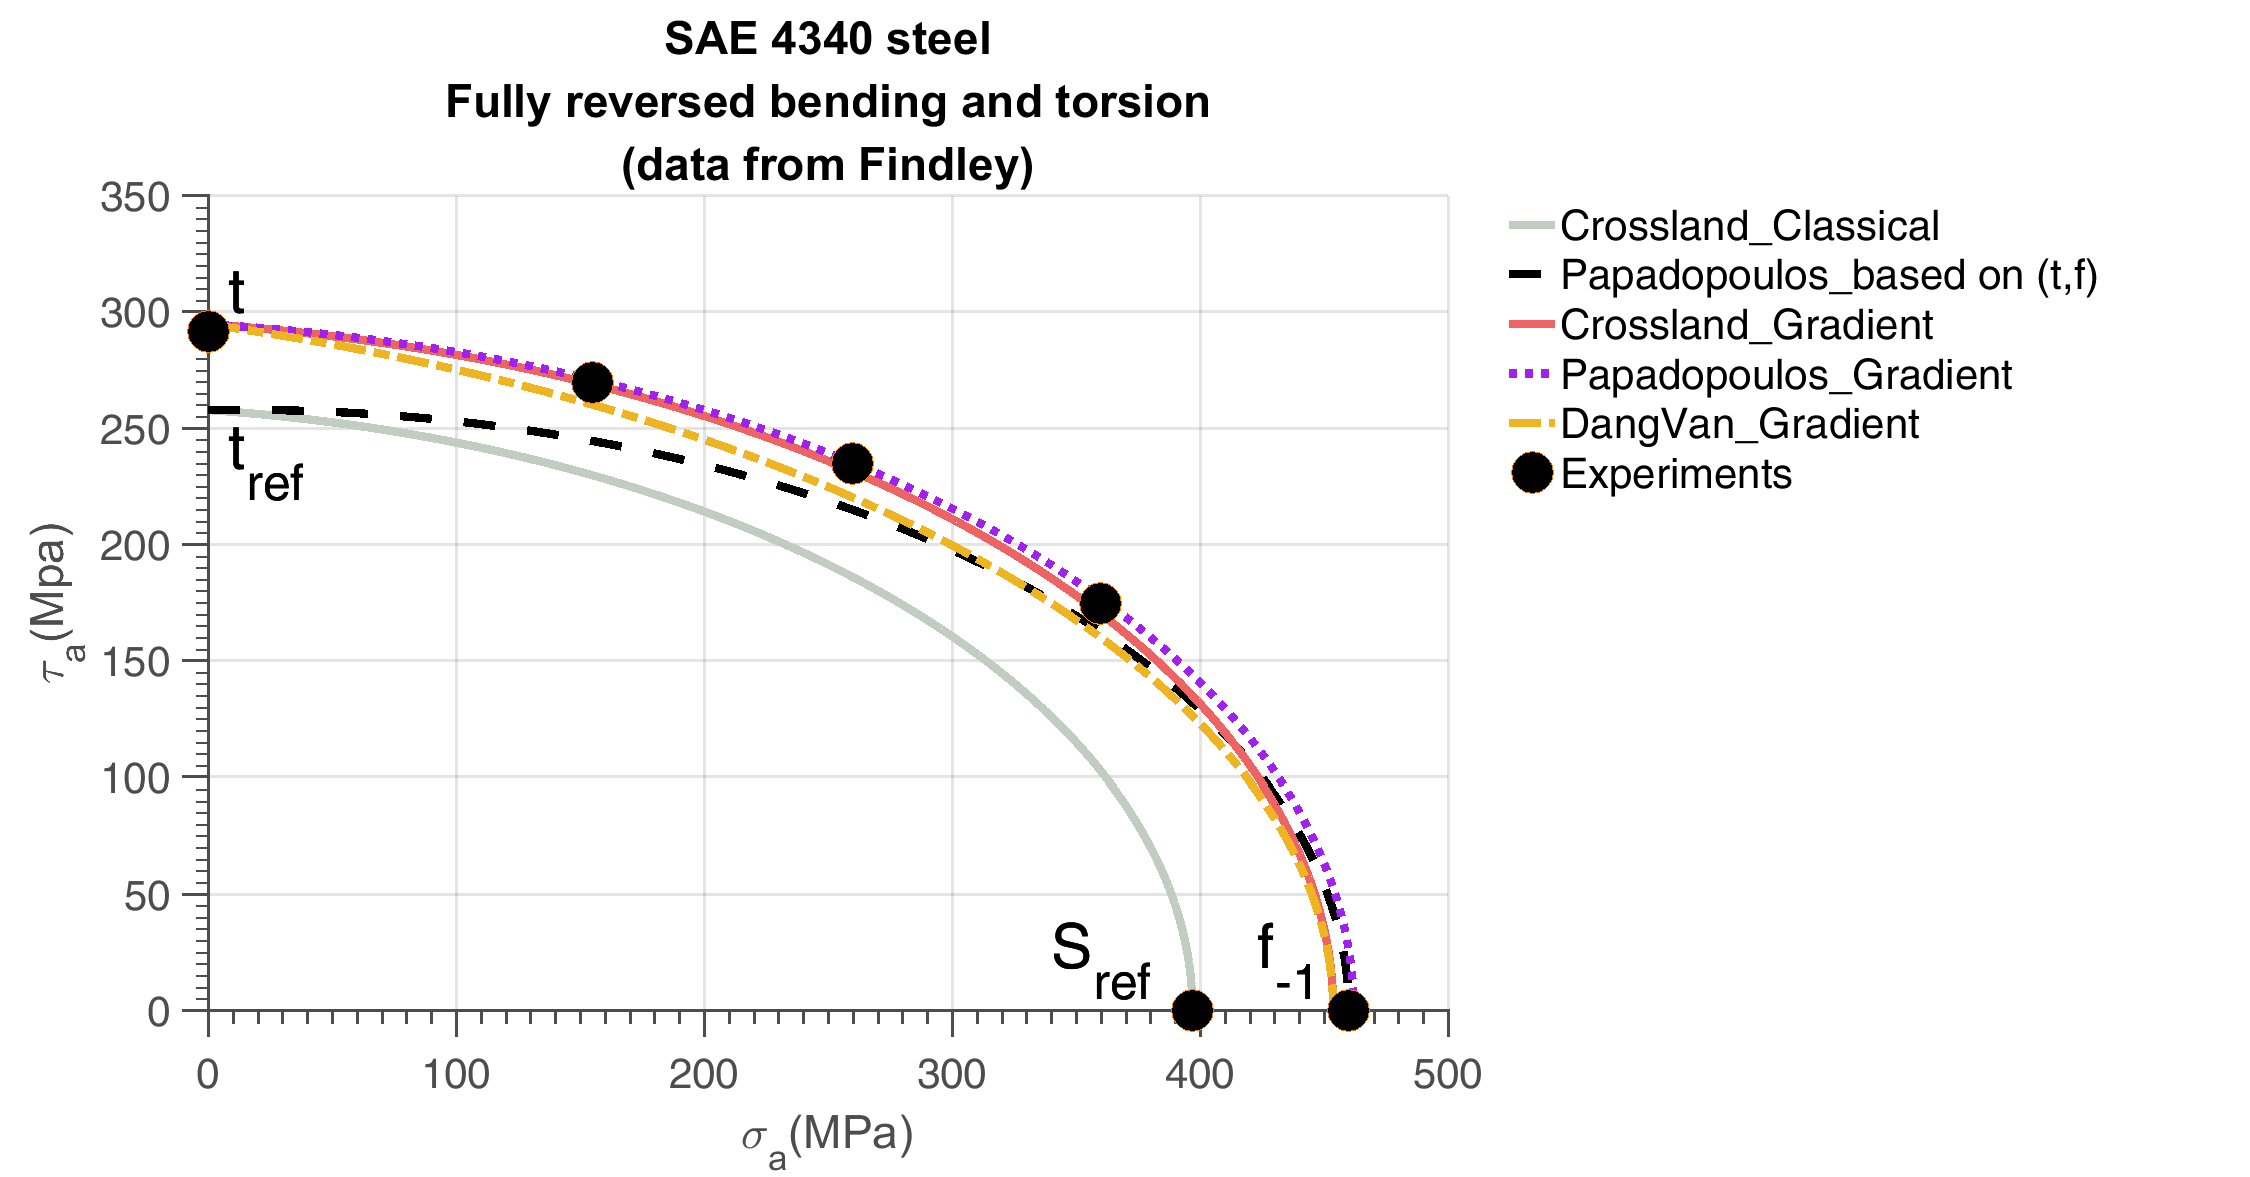
\includegraphics[width=\textwidth]{figures//4340.png}
	\caption{Fully reversed combined bending-twisting fatigue limit data (Findley et al.\cite{findley1956theory}, Papadopoulos and Panoskaltsis\cite{papadopoulos1996invariant}) compared with updated values computed with gradient effects with $l_g = 2.5 \, mm$.}
	\label{4340}
\end{figure}



\newpage
\subsection{Discussion}
\noindent\textbf{Remark 1} (Gradient terms). In this paper, the pure size effect has not been considered and only stress gradient effect is modeled. Whereas the latter is dominant rather than totally to the pure size effect as usually believed
\vspace{6pt} \\
\textbf{Remark 2} (Material characteristic length scale $l_g$). We study here the fatigue limit of macroscopic specimens and components for which the crack initiation is generally detected by loss of stiffness corresponding to crack length which can reach a millimeter. We choose $l_g$ ranging from $0.1$ to $2.5$mm(depending on crack nucleation definition). To verify the relevancy of this choice, we need more experimental data.
\vspace{6pt} \\
\textbf{Remark 3} (Extensions to other load case). This new criteria is generalized to multiaxial cases to capture
both well-known phenomena ‘‘Smaller is Stronger’’ and ‘‘Higher Gradient is Stronger’’ and thus can reproduce fatigue experimental data even at small scale.

\subsection{Conclusion}

The present study develops a simple formulation of gradient
multi-axial fatigue criteria extending the classical HCF criteria.
The objective is to model the surface gradient effects (yielding
apparent size and loading effects), which is not included yet in classical mechanics but become important at small scale or in the presence of notches, by taking into account just the gradient effect.  This is achieved by a simple and versatile technique, which we have validated on a few significative examples.  This effect allows us to discriminate between a compression tension test combined with a torsion test and a bending twisting test.  The extra cost is the apparition of a length scale $l_g$ which has to be determined by adequate experiments at different sizes. 

Nevertheless, in this work only simple fatigue tests have been examined. In these tests, the gradient has a beneficial effect on fatigue. However, cases where the effect can be presumably negative, especially under the circumstances of residual stresses, can be encountered. A reexamination and validation for complex loading could be perspective for this research direction. 

\section{Time varying load : the standard approach}
Fatigue failure is a damage accumulation process in which material property deteriorates continuously under
fatigue loading and the damage depends on the size of
stress and strain. With the accumulation of fatigue
damage, some accidents occur for these components. Research shows that a reliable lifetime prediction method is
particularly important in the design, safety assessments,
and optimization of engineering components and structures. Thus, it is important to formulate an accurate method
to evaluate the fatigue damage accumulation and effectively predict the fatigue life of these components.
The objective of this work is to contribute to the development life model that take into account the presence of complex variations of the stress tensor. We focus on Chaboche damage accumulation law in case of multiaxial high cycle fatigue. Heuristic formulations with different multiaxial fatigue criteria have been proposed. 

\subsection{The notion of damage in fatigue}


In the case of fatigue, we usually employ the concept of the loading cycle instead of time to evaluate the evolution of damage and to measure the fatigue lifetime. The equations then depend on the load through globally defined quantities over a cycle, such as amplitude, maximum value, mean value.
The growth equation of fatigue damage is therefore taken in the form:
$$\delta D=f(...)\delta N$$
$$\delta N=f\delta t$$
where $\delta t$ is a time sampling of the history in a given number of time intervals $\delta t_1,\delta t_2 ... \delta t_i, ...$ and $f$ is the mean frequency of those cycles during the considered time step.

\subsubsection{Linear and nonlinear accumulation of damage}
Cumulative effects, whether linear or nonlinear, are of great importance in fatigue. The rule of linear accumulation is in fact a property of any linear or nonlinear differential equation with separable variables. One approach to variable load histories uses the concept of fraction of life(also referred to as cycle ratio) used up by an event. These fractions are added together; when their sum reaches 1.0 or 100 percent we expect failure. This is the most common measure of damage, and is the quantifying measure we use here. 

The Palmgren-Miner linear rule as explained in \cite{lemaitre1990mechanics} is based on the assumption that damage is accumulated additively when it is defined by the associated life ratio $N_i/N_{Fi}$ where $N_i$ is the number of cycles applied under a given load for which the number of cycles to fracture(under periodic conditions) would be $N_{Fi}$. The fracture criterion is:
$$\sum_{i}N_i/N_{F_i}=1.$$
Therefore, in periodic tests, damage evolution is considered to be linear in that:
$$D=N/N_F.$$
For a test at two stress levels, the evolution is as shown schematically in \figref{linear accumulation}. In fact, the linear accumulation rule can be applied even to a damage which evolves nonlinearly. For this it is sufficient that a one-to-one relationship between $D$ and $N/N_F$ exists, or even that the damage evolution curve be a unique function(independent of the applied cycle) of the life ratio $N/N_F$ . 

There are, therefore, two ways of defining a damage incremental law incorporating the linear accumulation rule. It can be linear of the form and shown in \figref{linearevolution}:
$$\delta D= \delta N/N_F(...),$$
\begin{figure}[h!]
	\centering
	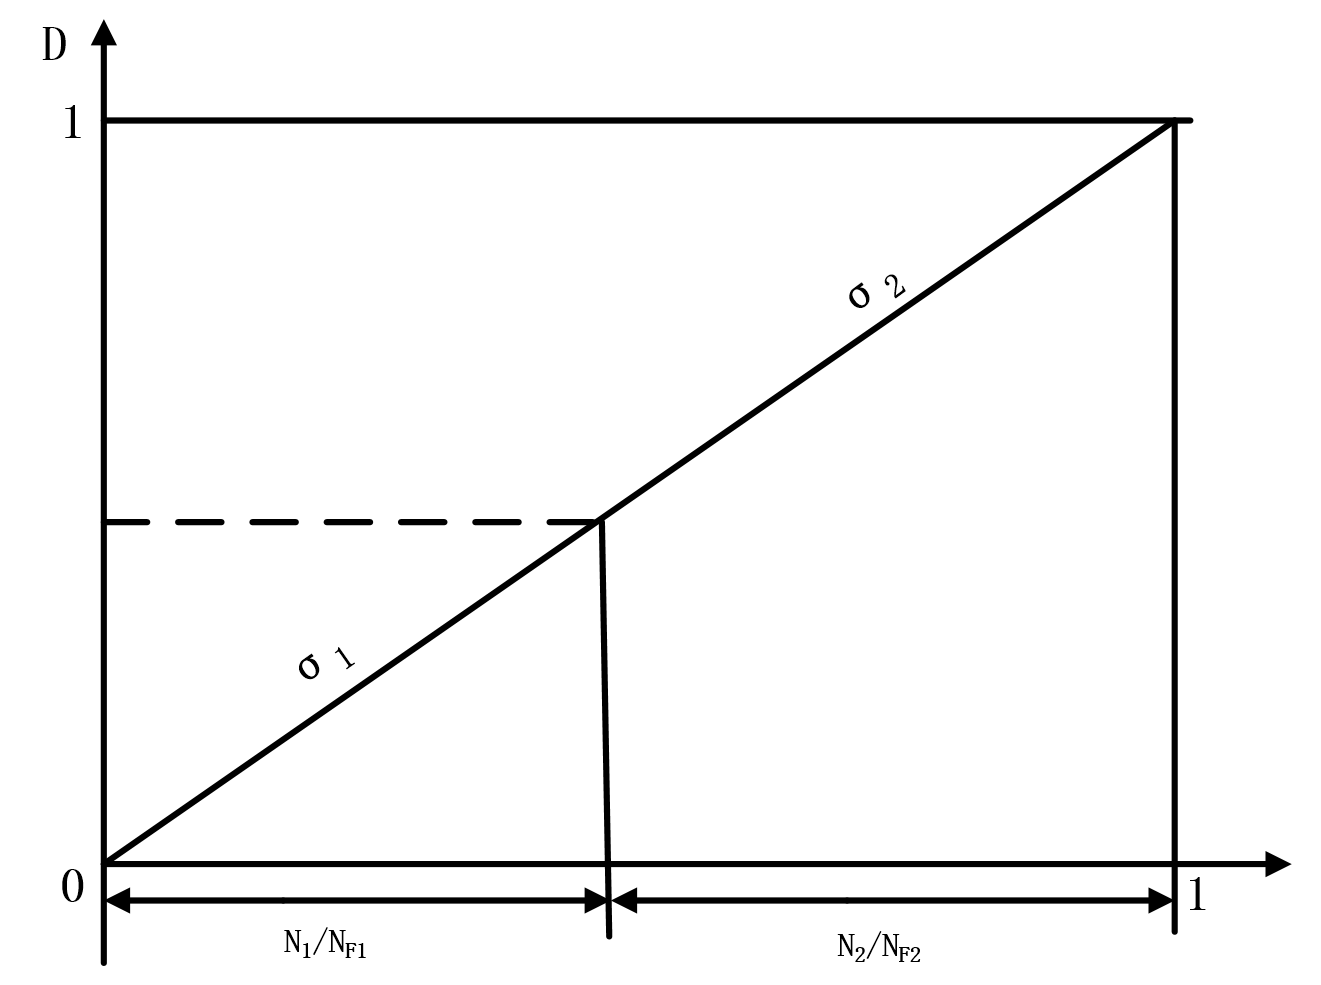
\includegraphics[width=0.8\textwidth]{figures//linearevolution.png} 
	\caption{Linear accumulation of damage with linear evolution}
	\label{linearevolution}
\end{figure}
where $N_F$ is the number of cycles to failure defined by the chosen parametric data.
The damage evolution can be nonlinear such as:
$$\delta D= \frac{(1-D)^{-k}}{k+1}\frac{\delta N}{N_F(...)}.$$
Here in any case, the damage evolution curve as function of life ratio $\delta N/N_F$ is supposed to be independent of the local state of stress (\figref{linear accumulation}).

In contrast, if the damage evolution curve,as a function of the life ratio $N/N_F$, depends on the applied loading we have the effect of nonlinear accumulation as shown in \figref{nonlinear accumulation}. There, $D_1$ represents the state of internal damage at the end of the first level $\sigma_1$. Evolution at the second level $\sigma_2$ continues from the same state, and it is clear that the sum of the life ratio is less than 1. From the point of view of the damage law, this nonlinearity always corresponds to the case where the variables which represent the load $\sigma$ and the damage variable $D$ have coupled evolution.

The Palmgren-Miner linear accumulation law gives good results only for loads for which there is little variation in the amplitude and mean value of stress. The assumption of linear damage is open to many objections. For example, sequence and interaction of events may have major influences on life, the rate of damage accumulation may depend on the load amplitude, experimental evidence often indicates that $\sum_{i}N_i/N_{F_i}\neq 1$ for a low-to-high or a high-to-low loading sequence.

\begin{figure}[h!]
	\begin{minipage}[t]{0.5\textwidth}
		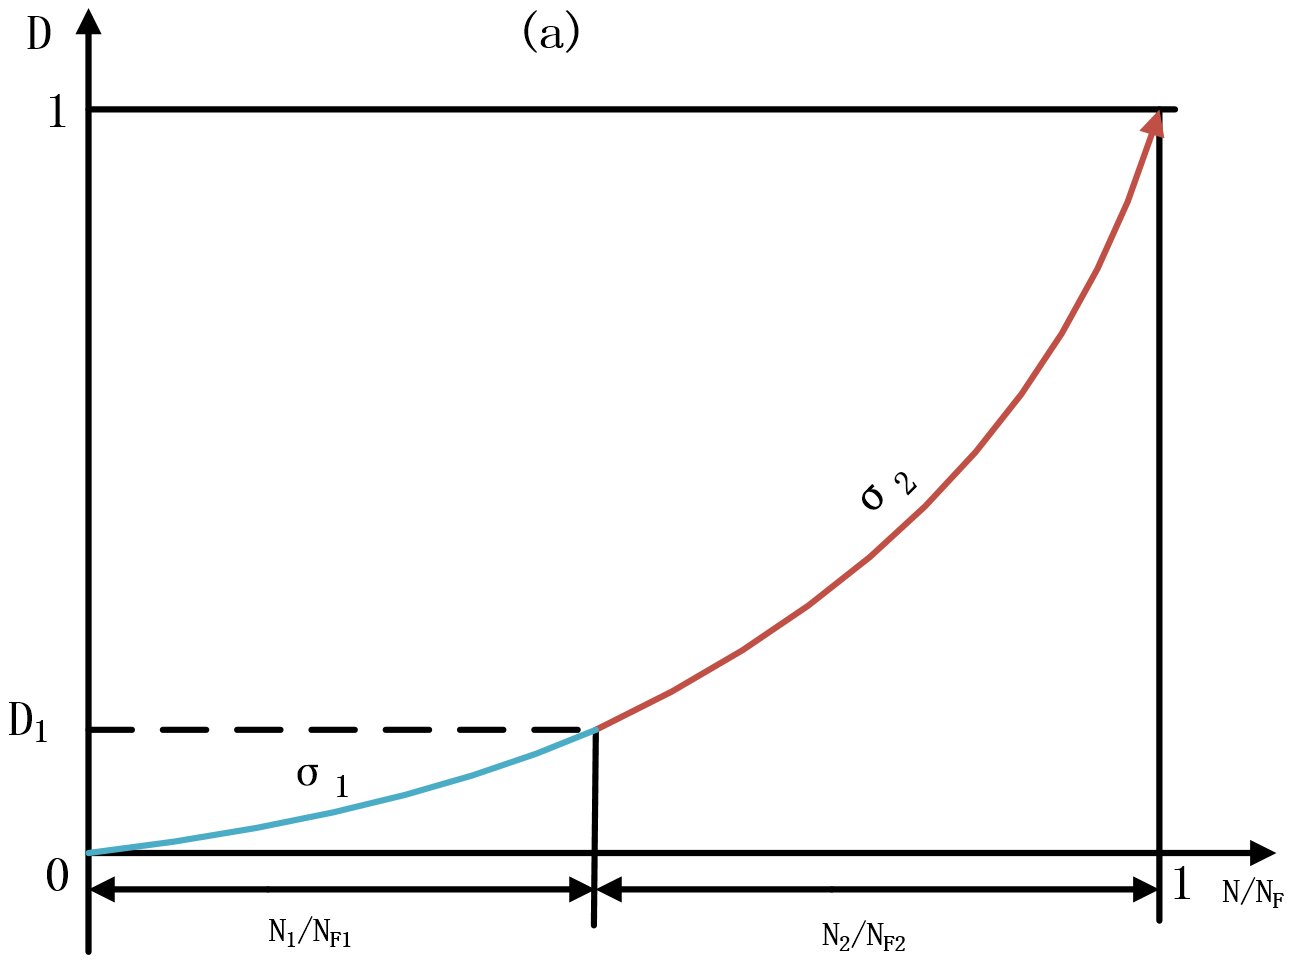
\includegraphics[width=\textwidth]{figures//linearaccumulation.png} 
		\caption{Damage with nonlinear evolution and linear accumulation}
		\label{linear accumulation}
	\end{minipage}
	\begin{minipage}[t]{0.5\textwidth}
		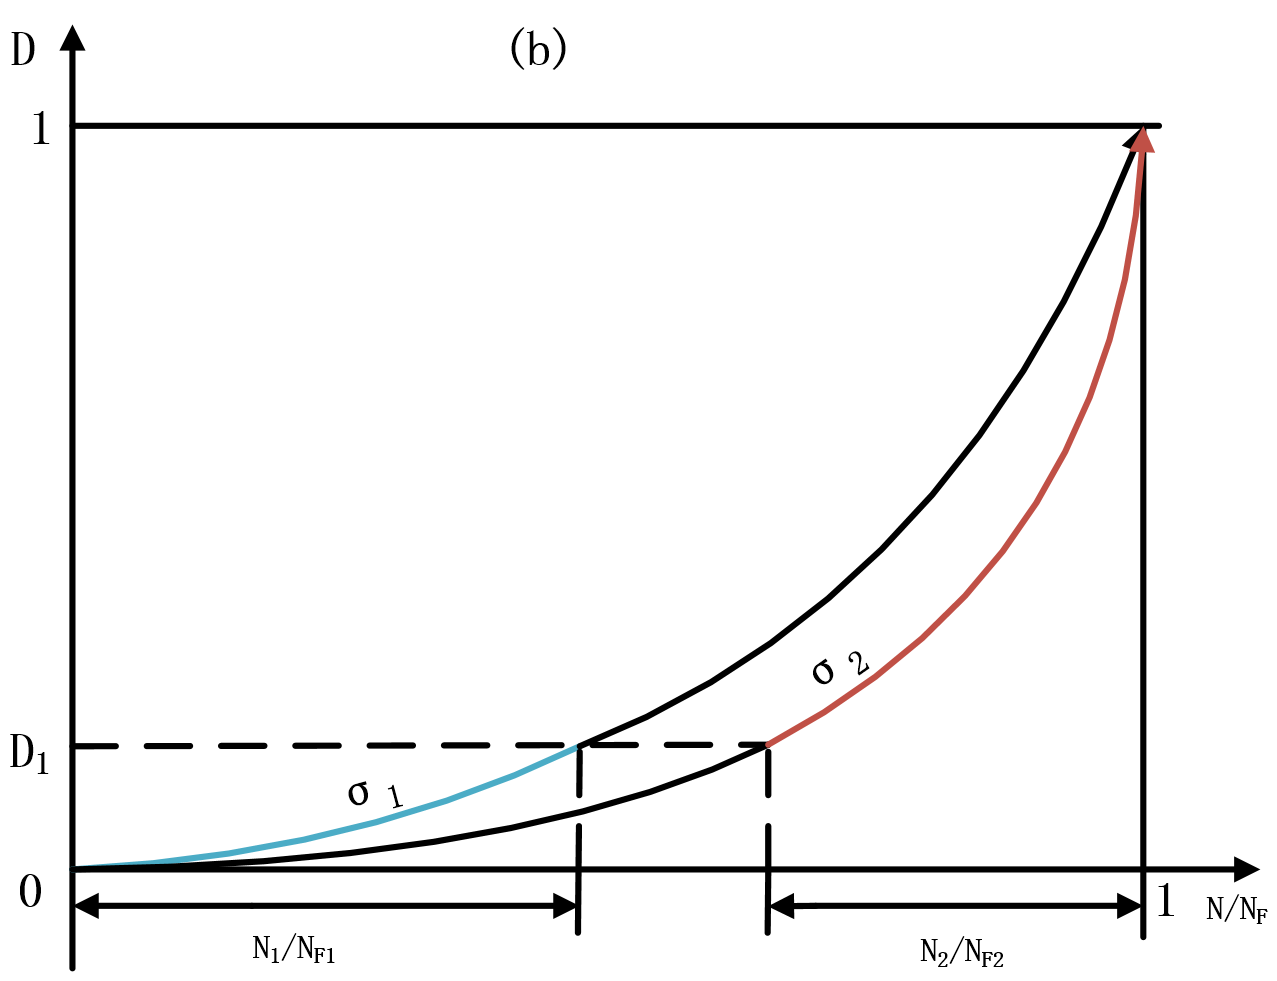
\includegraphics[width=\textwidth]{figures//nonlinearaccumulation.png} 
		\caption{Damage with nonlinear evolution and nonlinear accumulation}
		\label{nonlinear accumulation}
	\end{minipage}
\end{figure} 

\newpage
\subsubsection{Classic Chaboche damage law}

In periodic cyclic loadings, one way of writing a damage law which expresses the experimental results is to assume that the damage per cycle is a function of the maximum and the mean values of the stress:
$$\delta D/\delta N=f(\sigma_{Max},\sigma_m).$$
In order to recover, after integration, one of the many forms proposed to represent the Wohler curves, we let:
\begin{equation}
\delta D/\delta N=\frac{\sigma_{Max}-\sigma_l(\sigma_m)}{\sigma_{u}-\sigma_{Max}}(\frac{\sigma_{Max}-\sigma_m}{B(\sigma_m)})^{\gamma}.
\label{generalchaboche}
\end{equation}
with:

$\sigma_l(\sigma_m)=\sigma_m+s_{-1}(1-b\sigma_m)$ : mean stress component in the fatigue limit.

$B(\sigma_m)=B_0(1-b\sigma_m)$ : the mean stress component in the fatigue limit.

The number of cycles to failure is obtained by an obvious integration, with the condition:

$N=0 \to D=0$(initial undamaged state)

$N=N_F \to D=1$(macro-crack initiation)

so that by integration Eq.\eqref{generalchaboche} from $D=0$ to $D=1$ we get:
\begin{equation}N_F=\frac{\sigma_{u}-\sigma_{Max}}{\sigma_{Max}-\sigma_l(\sigma_m)}\left(\frac{\sigma_{Max}-\sigma_m}{B(\sigma_m)}\right)^{-\gamma}.
\label{NF}
\end{equation}

Eq.\eqref{generalchaboche} then writes:
$$\delta D=\delta N/N_F.$$

The constants are determined from conventional data:$\sigma_u$ is usually known, $s_{-1},b$ fit the results on the fatigue limits with relation $\sigma_l(\sigma_m)=\sigma_m+s_{-1}(1-b\sigma_m)$. Exponent $\gamma$ is collaborated from the S-N curve for reversed conditions, by plotting $\sigma_{Max}$ as function of $N_F(\sigma_{Max}-\sigma_l(\sigma_m))/(\sigma_{u}-\sigma_{Max})$, as deduced from Eq.\eqref{NF}. Coefficient $B(\sigma_m)$ is obtained from one point of the S-N curve.

\vspace{6pt}
\textbf{Uniaxial case}
\vspace{6pt}

The equation studied below allows us to describe the effects of nonlinear accumulation in the case of non-periodic cyclic loads\cite{FFE:FFE1}. A simple way to introduce such effects in the damage growth equation consists in rendering the load and damage variables non-separable. For example, we may take:
$$\delta D=D^{\alpha(\sigma_{Max},\sigma_m)}\left(\frac{\sigma_{Max}-\sigma_m}{C(\sigma_m)}\right)^\gamma\delta N$$
The exponent $\alpha$ depends on the loading $(\sigma_{Max},\sigma_m)$, which results in non-separability.

\vspace{6pt}
$$\alpha(\sigma_{Max},\sigma_m)=1-a\left\langle\dfrac{\sigma_{Max}-\sigma_l(\sigma_m)}{\sigma_u-\sigma_{Max}}\right\rangle$$
\vspace{6pt}

$$ M(\sigma_m)=M_0(1-b\sigma_m)$$ 
\vspace{6pt}

The exponent $\alpha$ represents the internal variables(for example the hardening state of the material), which depends on the loading $(\sigma_{Max},\sigma_m)$, resulting in non-separability. $\alpha$  allows a non-linear damage cumulative rule as it is experimentally observed. a and $\gamma$ are material parameters.$M_0$ represent the fatigue limit and the static fracture. The coefficients $\gamma$ and $M_0$ are determined from these experimental Woehler's curves by plotting Eq.\eqref{eqnf} and take one point from it. 

The concept of effective stress applied to fatigue provides an indirect measure. The measured evolutions are extremely nonlinear. With this concept, damage can really be measured only in the last part of the life-time, when microscopic initiations have already occurred(this is the phase of micro-propagation of defects). And these damage evolutions are extremely nonlinear. To reproduce this phenomenological aspect it is sufficient to make a change of variable by replacing $D$ in the previous equation by:
$$1-(1-D)^{\gamma+1}.$$
The differential law can be written as:
\begin{equation}\delta D=[1-(1-D)^{\gamma+1}]^{\alpha(\sigma_{Max},\sigma_m)}\big[\frac{\sigma_{Max}-\sigma_m}{M(\sigma_m)}\big]^\gamma\delta N
\label{diff}
\end{equation}

This form is more complex, but its properties are identical to the properties of the previous equation, except for the current value of damage. Now we integrate it to see how damage $D$ evolves with cycle numbers $N$ and the influence of different parameters. By differential calculus, we get from Eq.\eqref{diff}:
\begin{equation}\delta [1-(1-D)^{\gamma+1}]^{1-\alpha}=(1-\alpha)(\gamma+1)\big[\frac{\sigma_{Max}-\sigma_m}{M(\sigma_m)}\big]^\gamma\delta N
\label{easyintegration}
\end{equation}


The number of cycles to failure, obtained by integrating $D$ from 0 to 1 is:
\begin{equation}N_F=\frac{1}{(\gamma+1)(1-\alpha)}\left(\frac{\sigma_{Max}-\sigma_m}{M(\sigma_m)}\right)^{-\gamma}
\label{eqnf}
\end{equation}
and we find that $M(\sigma_m)=C(\sigma_m)(\gamma+1)^{1/\gamma}$. 
In differential form, the relation \eqref{diffform} writes from Eq.\eqref{easyintegration} and Eq.\eqref{eqnf}:
\begin{equation}\delta [1-(1-D)^{\gamma+1}]^{1-\alpha}=\frac{\delta N}{N_F}
\label{diffform}
\end{equation}
When we integrate Eq.\eqref{easyintegration} from $0$ to $D$ at constant loading conditions. The damage, expressed as a function of $N/N_F$ is:
\begin{equation}D=1-\left[ 1-\left( \frac{N}{N_F}\right) ^{\frac{1}{1-\alpha}}\right] ^{\frac{1}{\gamma+1}}.
\end{equation}
This expression is in good agreement with experimental results\cite{lemaitre1990mechanics}. 



\vspace{6pt}
\textbf{Multiaxial case}
\vspace{6pt}

The applied stress and strain tensors are often multiaxial and present a complex path during a loading cycle. In the case of multiaxial loading fatigue, the Chaboche model is represented by the following equation:
\begin{equation}\delta D = \left( 1 -(1-D)^{\gamma+1}\right)^\alpha \left(\frac{\widetilde{A}_{\uppercase\expandafter{\romannumeral2}}}{M(\sigma_H)}\right)^\gamma \delta N
\label{chabochemulti}
\end{equation} 
Where the amplitude $\sigma_{Max}-\sigma_l(\sigma_m)$ is replaced by the deviatoric norm $A_{\uppercase\expandafter{\romannumeral2}}$ and the average stress is replaced by the hydrostatic pressure. We should note that for an isotropic damage theory:
$$\widetilde{A}_{\uppercase\expandafter{\romannumeral2}}=A_{\uppercase\expandafter{\romannumeral2}}/(1-D)$$

\begin{equation}\alpha = 1 - a\left\langle \frac{A_{\uppercase\expandafter{\romannumeral2}} - A_{\uppercase\expandafter{\romannumeral2}}^\ast(\sigma_H)}{ \sigma_{u} - \sigma_{eqMax}}\right\rangle.\end{equation}

$\alpha$ represents the internal variables,characterizes the non-linearity of the damage evolution, defines
the non-linear cumulation, and allows to take into account the mean stress effect and describes the damage occurrence of the material: as long as $\alpha < 1$, there is damage creation. The coefficient $a$ gives the amount of fragility which is suggested by a given occurrence of fatigue limit violation.

$A_{\uppercase\expandafter{\romannumeral2}}$ is the amplitude of octahedral shear stress given by:

\begin{equation}A_{\uppercase\expandafter{\romannumeral2}}=\frac{1}{2}\max\limits_{t}\sqrt{\frac{1}{2}\uline{\uline{\Delta s}}:\uline{\uline{\Delta s}}}=\sqrt{J_2}_a=\frac{1}{2}\Delta\sigma_{eqmax},\end{equation}

The quantity $A_{\uppercase\expandafter{\romannumeral2}}^\ast(\sigma_H)$ represents the infinite life fatigue limit. For example,the Sines fatigue limit criterion is formulated by the following equation:
\begin{equation} A_{\uppercase\expandafter{\romannumeral2}}^\ast(\sigma_H)=s_{-1}(1-3b\sigma_H).\end{equation}

Above, $s_{-1}$ and $\sigma_{u}$ are respectively the fatigue limit at zero mean stress and the ultimate tensile stress. For steel, normally $s_{-1}\approx 0.48\sigma_{u}$.

The function $M(\sigma_H)$ in Eq.\eqref{chabochemulti} quantifies the mean stress effect through Low Cycle Fatigue(LCF) loading range:
$$M(\sigma_H)=s_{-1}\left(1-3\frac{\sigma_H}{\sigma_u}\right).$$

We can get the $D-N$ curve in \figref{DN} by integrating Eq.\eqref{chabochemulti}. This is in the case of constant loading conditions because we regard $\alpha$ and $\gamma$ as invariable parameters.
\begin{equation}N =\frac{( 1 -(1-D)^{\gamma+1})^{1-\alpha}}{(1+\gamma)(1-\alpha)}\left[\frac{A_{\uppercase\expandafter{\romannumeral2}}}{M(\sigma_H)}\right]^{-\gamma} 
\label{D-N}
\end{equation} 

\begin{figure}[h!]
	\centering
	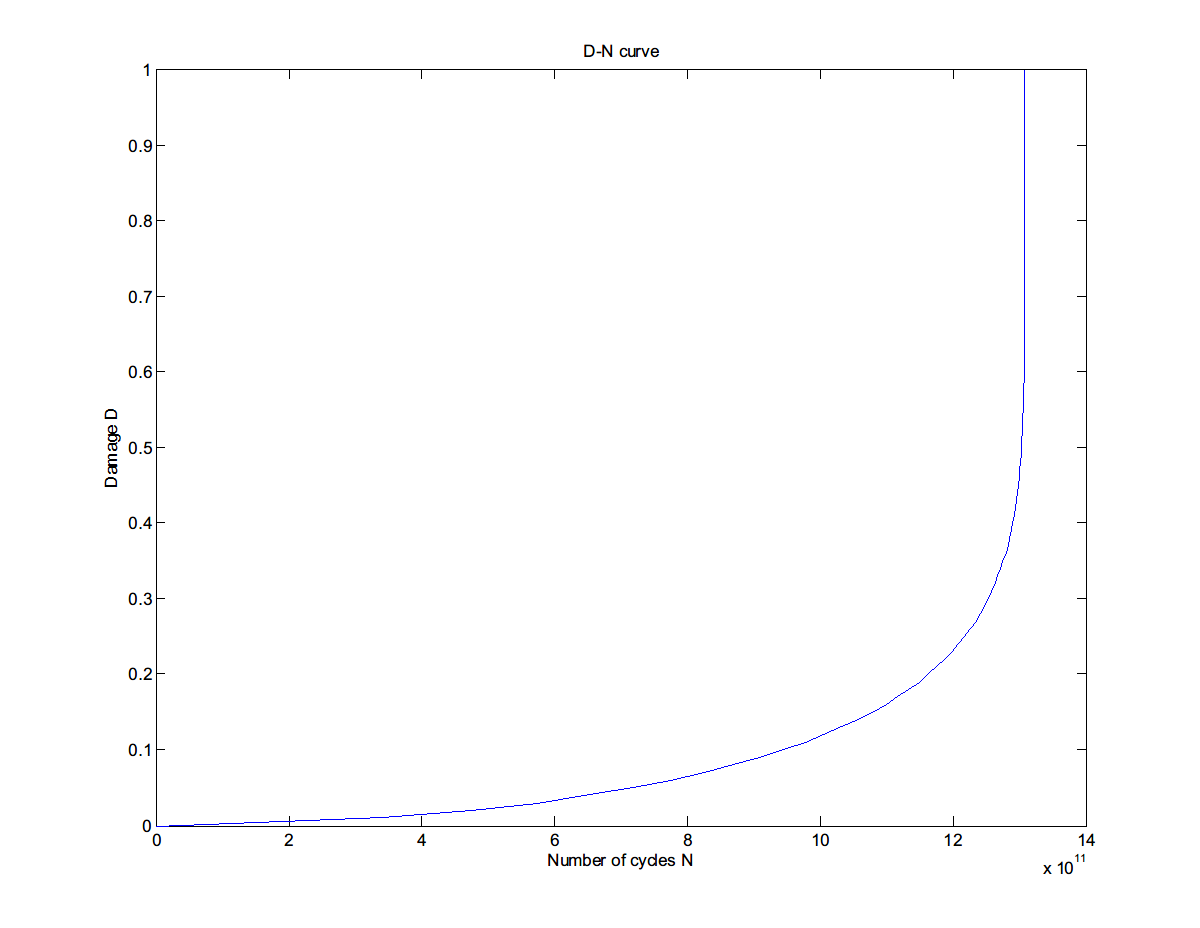
\includegraphics[width=0.8\textwidth]{figures//D-N.png} 
	\caption{Damage accumulation in terms of N in constant loading condition, with D and N are related by the evolution equation \eqref{D-N}}
	\label{DN}
\end{figure}

The number of cycles to failure, obtained at $D=1$, is: 
\begin{equation}N_F = \frac{1}{(\gamma+1)(1-\alpha)}\left[\frac{\widetilde{A}_{\uppercase\expandafter{\romannumeral2}}}{M(\sigma_H)}\right]^{-\gamma}
\label{chaboche}
\end{equation} 

It should be noted that in multiaxial case the effective stress amplitude is written as:
$$A_{\uppercase\expandafter{\romannumeral2}}=\frac{\widetilde{A}_{\uppercase\expandafter{\romannumeral2}}}{(1-D)}$$
In Eq.\eqref{chaboche}, $\gamma$, $b$ and $a$ are material parameters determined from fatigue tests.

In the case of multiaxial fatigue loading, an infinite life is obtained if the stress amplitude $A_{\uppercase\expandafter{\romannumeral2}}$ respects:

\begin{equation}A_{\uppercase\expandafter{\romannumeral2}}\leqslant A_{\uppercase\expandafter{\romannumeral2}}^\ast(\sigma_H)=s_{-1}(1-3b\sigma_H).\end{equation}

In terms of Sines criterion which Chaboche uses, it writes:
\begin{equation}\sqrt{J_2}_a+3bs_{-1}\sigma_H-s_{-1}\leqslant 0.
\label{sines}
\end{equation}

$\sigma_H$ is the mean hydrostatic stress defined by:
\begin{equation}\sigma_H=\frac{1}{6}[\max tr(\uline{\uline{\sigma}}(n))+\min tr(\uline{\uline{\sigma}}(n))],\end{equation}


The damage is expressed the same as in uniaxial case:
\begin{equation}D=1-\left[ 1-\left( \frac{N}{N_F}\right) ^{\frac{1}{1-\alpha}}\right] ^{\frac{1}{\gamma+1}}.
\label{damage}
\end{equation}

\begin{figure}[h!]
	\centering
	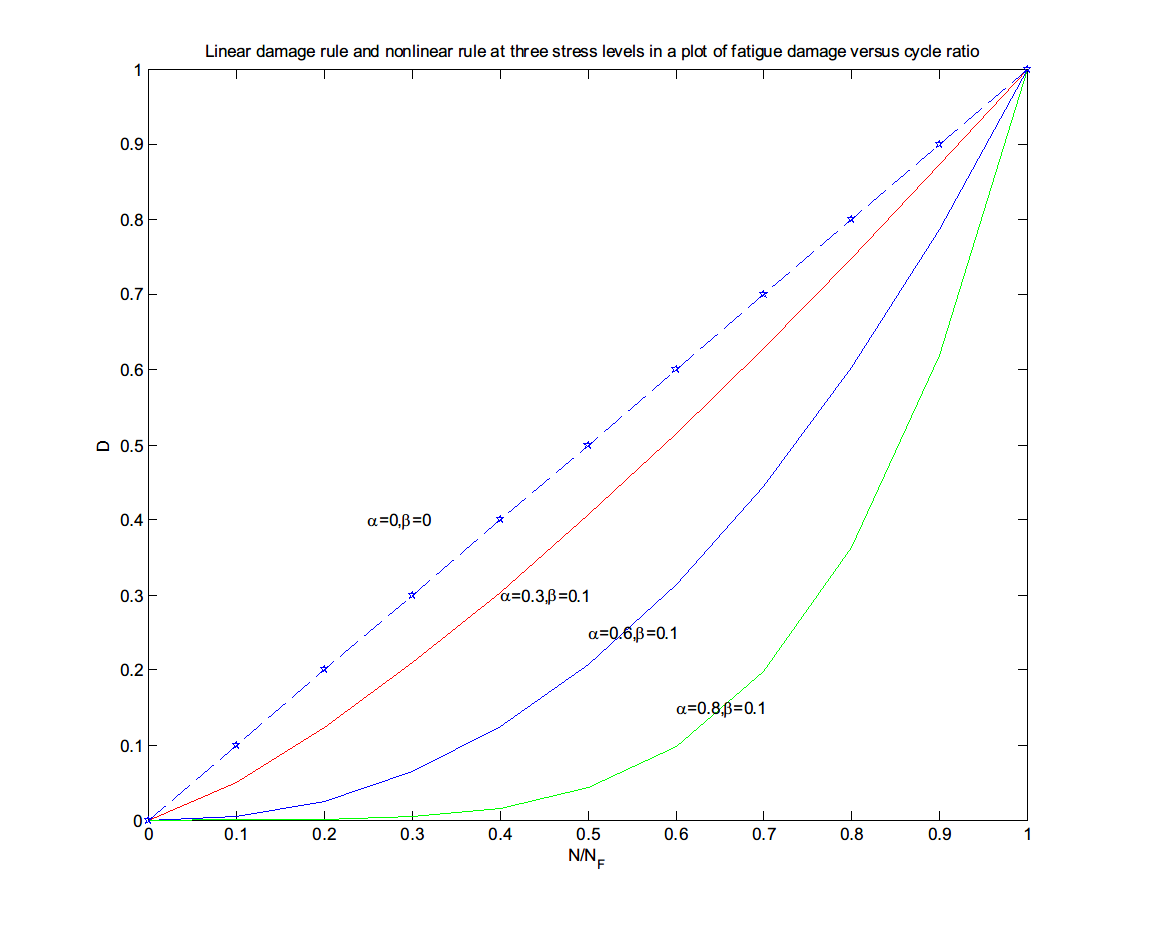
\includegraphics[width=\textwidth]{figures//Dratio1.png}
	\vspace{-12pt}
	\caption{Influence of function $\alpha$ in a plot of fatigue damage versus cycle ratio with $\gamma=0.1$}
	\label{Alpha}
\end{figure}
These theories account for the nonlinear nature of fatigue damage accumulation by using nonlinear relations such as Eq.\eqref{damage} where the power $\alpha$ depends on the load level(see \figref{Alpha}).


\begin{figure}[h!]
	\centering
	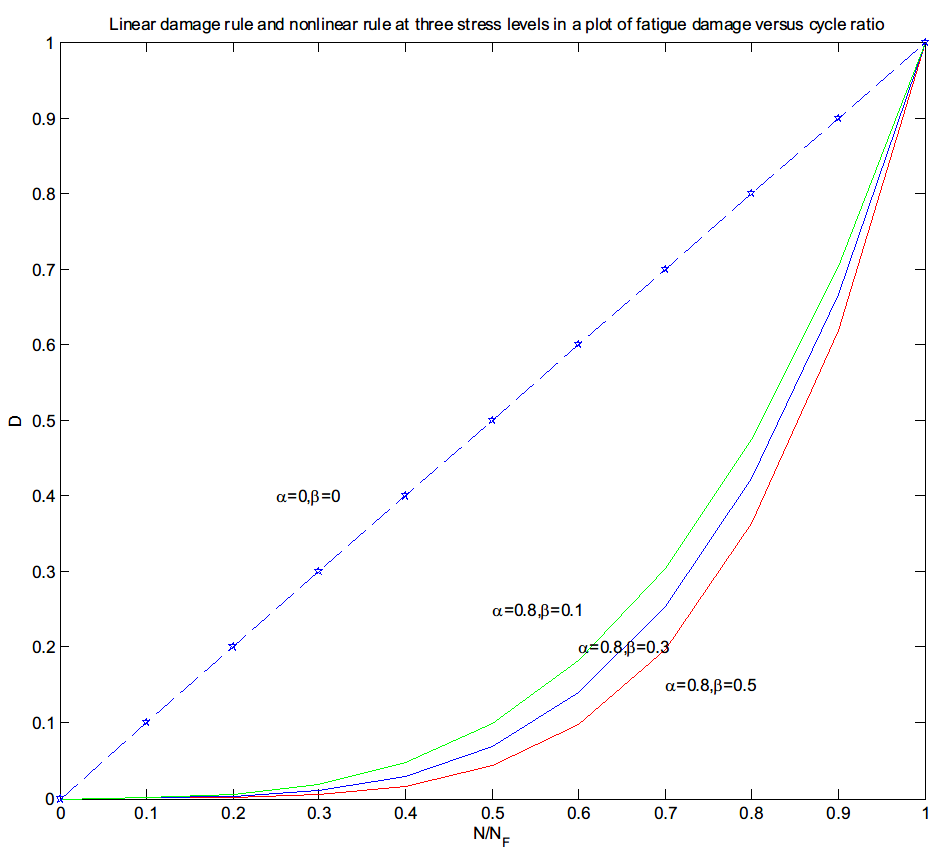
\includegraphics[width=0.8\textwidth]{figures//Dratio2.png}
	\vspace{-12pt}
	\caption{Influence of function $\gamma$ in a plot of  damage versus fatigue life ratio with $\alpha=0.8$}
\end{figure}

\clearpage
\subsection{Verification method of Chaboche law}

Many fatigue damage accumulation models are based on the two level loading experiments which is one of the basic random loading analysis. To facilitate our verification of the law we use two-stress level loading, the specimen is firstly loaded at stress $\sigma_1$ for $N_1$ cycles and then at stress $\sigma_2$ for $N_2$ cycles until failure. We can then observe if the experimental results are satisfactory.\\
After $N_1$ cycles, we have from Eq.\eqref{damage}, a damage $D_1$ given by:
\begin{equation}
[1-(1-D_1)^{\gamma+1}]^{1-\alpha_1}=\frac{N_1}{N_{F1}}
\label{23a}
\end{equation}
By integrating Eq.\eqref{diffform} from $D=D_1$ to $D=1$, we get:
\begin{equation}
1-[1-(1-D_1)^{\gamma+1}]^{1-\alpha_2}=\frac{N_2}{N_{F2}}
\end{equation}
Which yields:
\begin{equation}1-\frac{N_2}{N_{F2}}=1-[1-(1-D_1)^{\gamma+1}]^{1-\alpha_2}
\label{23b}
\end{equation}
From Eq.\eqref{23a} and Eq.\eqref{23b}, after elimination of $[1-(1-D_1)^{\gamma+1}]$ we get:
\begin{equation} \frac{N_2}{N_{F2}}=1-(\frac{N_1}{N_{F1}})^\frac{1-\alpha_2}{1-\alpha_1}=1-(\frac{N_1}{N_{F1}})^\eta\end{equation}
with
\begin{equation}\eta=\frac{1-\alpha_2}{1-\alpha_1}=
\frac{A_{\uppercase\expandafter{\romannumeral2 2}} - A_{\uppercase\expandafter{\romannumeral2}}^\ast(P_{m2})}{A_{\uppercase\expandafter{\romannumeral2 1}} - A_{\uppercase\expandafter{\romannumeral2}}^\ast(P_{m1})}\frac{ \sigma_{u} - \sigma_{eqMax1}}{ \sigma_{u} - \sigma_{eqMax2}}=
\frac{\sqrt{J_{2,a_2}} - s_{-1}(1-3bP_{m_2})}{\sqrt{J_{2,a_1}} - s_{-1}(1-3bP_{m_1})}\frac{ \sigma_{u} - \max(2\sqrt{J_{2,a_1}})}{  \sigma_{u} - \max(2\sqrt{J_{2,a_2}})}
\label{eq.eta}
\end{equation}

In the case of high-low loading sequence($\sigma_1>\sigma_2$):

$$\eta=\frac{1-\alpha_2}{1-\alpha_1}<1;\frac{N_2}{N_{F2}}=1-(\frac{N_1}{N_{F1}})^\eta<1-\frac{N_1}{N_{F1}};\frac{N_1}{N_{F1}}+\frac{N_2}{N_{F2}}<1$$

The cumulative damage under high-low loading sequence, as we deduced, has the addition of partial lives less than unit. 

Similarly, the cumulative damage under low-high loading sequence has addition of partial lives more than 1. 
$$\frac{N_1}{N_{F1}}+\frac{N_2}{N_{F2}}>1$$

For constant two-level stress loading, $\alpha_1=\alpha_2$, the Chaboche law returns to the Miner rule where:
$$\frac{N_1}{N_{F1}}+\frac{N_2}{N_{F2}}=1$$
\subsection{Chaboche law containing different criteria}
\subsubsection{Chaboche law with Crossland criterion}

In the previous model we used Sines fatigue criterion constructing the damage criterion exponent $\alpha$. Now we want to see Chaboche law with different criteria and compare the numerical results. Firstly, $\alpha$ represents the internal variables and contains the fatigue criterion, so we first change $\alpha$ to satisfy Crossland Criterion:

\begin{equation}\alpha = 1 - a\left\langle \frac{\max\limits_{n}\sqrt{J_2}_a(n)+a_c{P_{max}(n)}-b_c}{ \sigma_{u} - 2\max\sqrt{J_2}_a}\right\rangle.\end{equation}

with
\begin{equation}
a_c=\frac{(t_{-1}-\frac{f_{-1}}{\sqrt{3}})}{\frac{f_{-1}}{3}}, \quad 
b_c=t_{-1}.
\end{equation}

\begin{equation}\eta_c=\frac{1-\alpha_2}{1-\alpha_1}=
\frac{\sqrt{J_{2,a_2}}+a_cP_{M_2}-b_c}{\sqrt{J_{2,a_1}}+a_cP_{M_1}-b_c}\frac{ \sigma_{u} - \max(2\sqrt{J_{2,a_1}})}{  \sigma_{u} - \max(2\sqrt{J_{2,a_2}})}
\end{equation}

In Eq.\eqref{D-N}, the amplitude of octahedral shear stress $A_{\uppercase\expandafter{\romannumeral2}}$ remain unchanged.

\subsubsection{Chaboche law with Dang Van criterion}

We change $\alpha$ to express it through Dang Van Criterion:

\begin{equation}\alpha = 1 - a\left\langle \frac{\max\limits_{n}\left\{\tau{(n)}+a_DP{(n)}\right\}-b_D}{ \sigma_{u} - 2\max\sqrt{J_2}_a}\right\rangle.\end{equation}

with
\begin{equation}
\tau(n)=\frac{1}{2}(\hat{\sigma}_{\Rmnum{1}}(n)-\hat{\sigma}_{\Rmnum{3}}(n))
\end{equation}
$$a_D=\frac{3t_{-1}}{f_{-1}}-\frac{3}{2}, b_D=t_{-1}.$$

\begin{equation}\eta_D=\frac{1-\alpha_2}{1-\alpha_1}=
\frac{\max\limits_{t}\left\{\tau_2{(n)}+a_DP_2{(n)}\right\}-b_D}{\max\limits_{t}\left\{\tau_1{(n)}+a_DP_1{(n)}\right\}-b_D}\frac{ \sigma_{u} - \max(2\sqrt{J_{2a_1}})}{  \sigma_{u} - \max(2\sqrt{J_{2a_2}})}
\end{equation}
In Eq.\eqref{D-N}, we proposed to change $A_{\uppercase\expandafter{\romannumeral2}}$ to $max\tau(n)$:
\begin{equation}N_F = \frac{1}{(\gamma+1)(1-\alpha)}\left[\frac{max\tau(n)}{M(\sigma_H)}\right]^{-\gamma}
\label{dvchaboche}
\end{equation} 

\subsection{Numerical testing on different loading patterns}
The fatigue limit with different criteria are distinctive. We compare different criteria in a $A_{\uppercase\expandafter{\romannumeral2}}-N_F$ figure as predicted in Eq.\eqref{chaboche}. Here
$\gamma$, $b$ and $a$ are material parameters determined from fatigue tests.

In this case we have 
$$N_F = \frac{1}{(\gamma+1)(1-\alpha)}\left[\frac{A_{\uppercase\expandafter{\romannumeral2}}}{M(\sigma_H)}\right]^{-\gamma},$$

$$M(\sigma_H)=s_{-1}\left(1-3\sigma_H/\sigma_u\right).$$

For Sines and Crossland criteria:

$$A_{\uppercase\expandafter{\romannumeral2}}=\sqrt{J_2}_a=\frac{1}{2}\max\limits_{t}\sqrt{\frac{1}{2}(\Delta s_{11}^2+\Delta s_{22}^2+\Delta s_{33}^2+2\Delta s_{12}^2+2\Delta s_{13}^2+2\Delta s_{23}^2)}.$$

For Dang Van criterion:
$$A_{\uppercase\expandafter{\romannumeral2}}= max\tau(n).$$ 

\newpage
\subsubsection{Test on pure rotation}

From the fatigue zone we select $r=0.1$ as the radius to study. We select here:

$s_{-1}=f_{-1}=0.8MPa$,

$\sigma_{u}=1.67MPa$ 

$\gamma=6$


$A_{\uppercase\expandafter{\romannumeral2}}-N_F$ figure is shown in \figref{JNrotation}. 
\begin{figure}[h!]
	\centering
	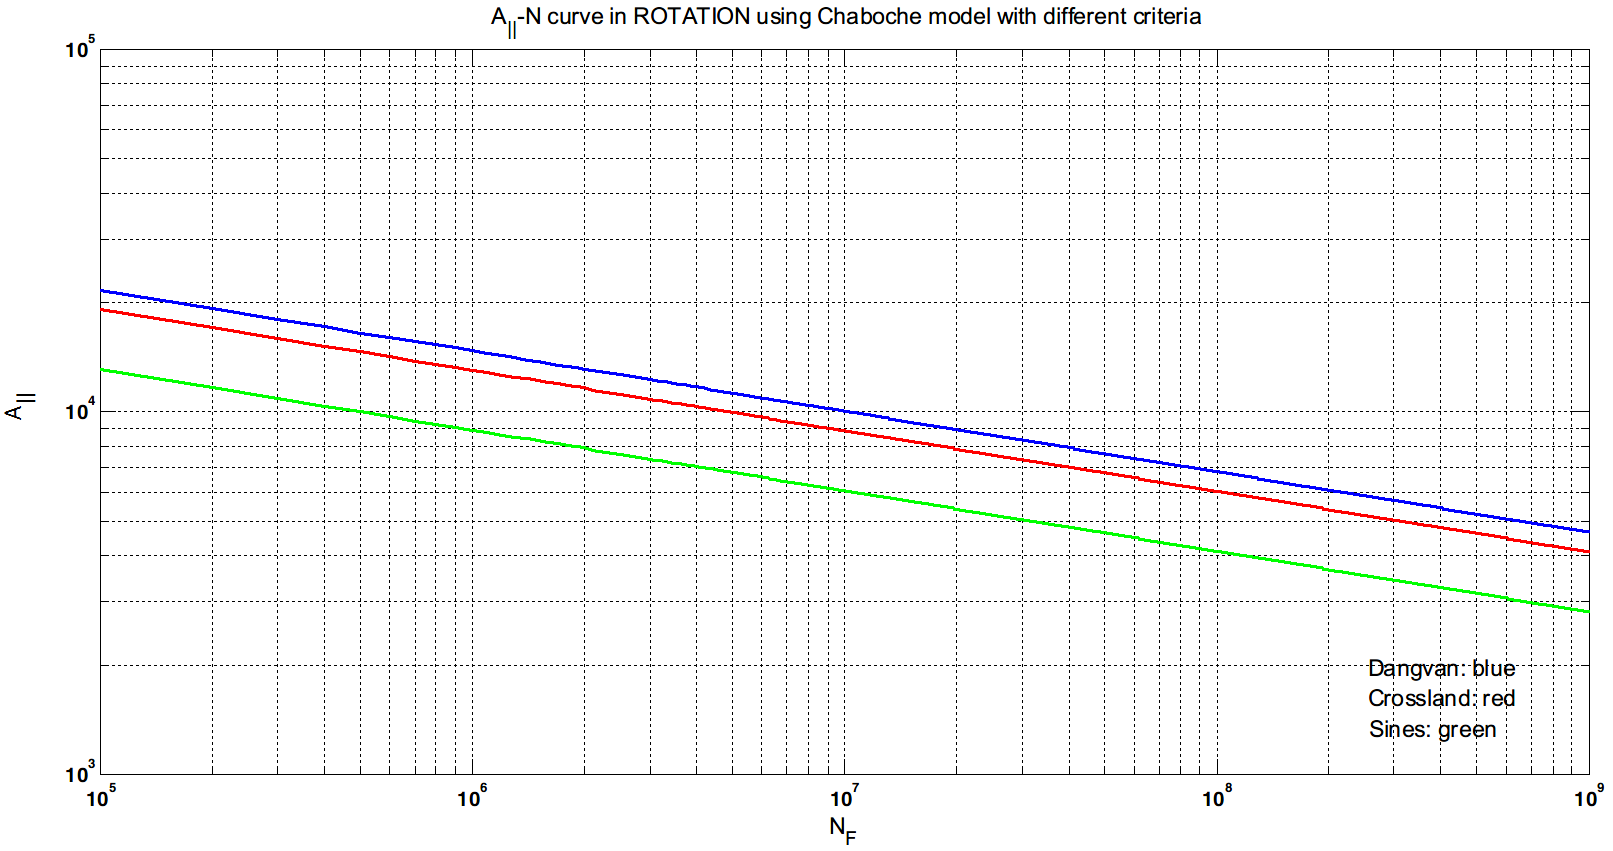
\includegraphics[width=\textwidth]{figures//JNrotation.png} 
	\caption{$A_{\uppercase\expandafter{\romannumeral2}}-N_F$ curve in rotation at r=0.1}
	\label{JNrotation}
\end{figure}

In pure rotation, we assume the first and second rotating speed are respectively $w_1=20rpm$ and $w_2=15rpm$.  

\vspace{6pt}
$A_{\uppercase\expandafter{\romannumeral2}1}=\sqrt{J_{2,a_1}}=7.7606E5 Pa$

\vspace{6pt}
$A_{\uppercase\expandafter{\romannumeral2}2}=\sqrt{J_{2,a_2}}=4.3653E5 Pa$

\vspace{6pt}
$P_{m_1}=8.8342E5 Pa$

\vspace{6pt}
$P_{m_2}=4.9693E5 Pa$

Substituting the above to Eq.\eqref{eq.eta} we can get $\eta$ in High-Low sequence:
$$\eta_1=0.0721,$$

in Low-High sequence:
$$\eta_2=13.8654.$$

The predicted results are shown in \figref{2stressR}.

\begin{figure}[h!]
	\centering
	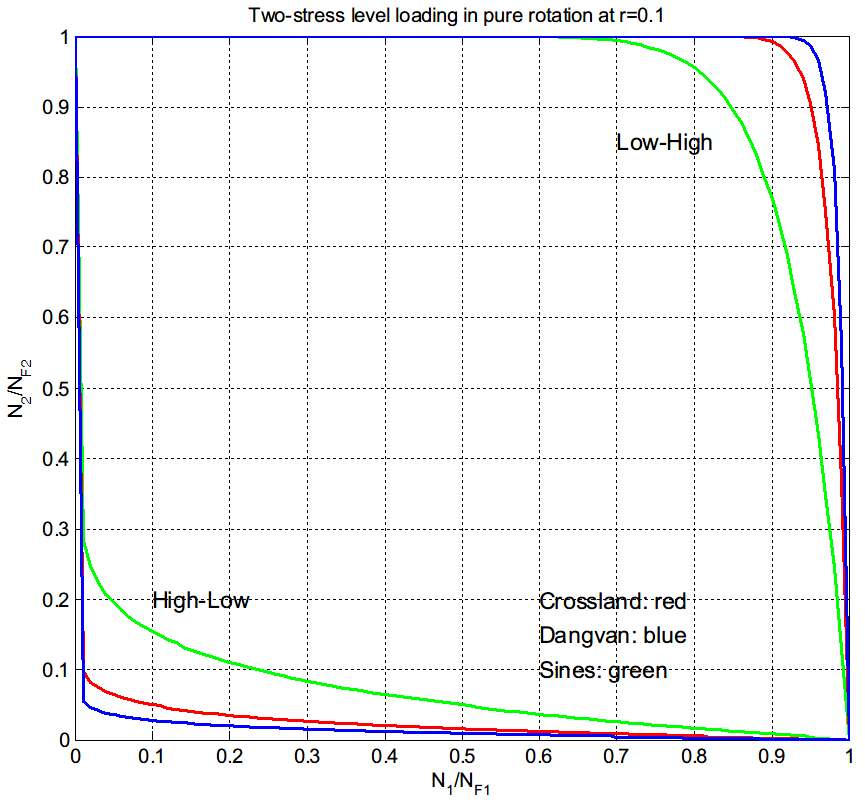
\includegraphics[width=\textwidth]{figures//2stressR.png} 
	\caption{Two-stress level loading in pure rotation at r=0.1}
	\label{2stressR}
\end{figure}

\newpage
\subsubsection{Test on 4-point bending}
From the fatigue zone we select $y=3$ to study. We select here:

$s_{-1}=f_{-1}=0.8MPa$,

$\sigma_{u}=1.67MPa$ 

$\gamma=6$

The $A_{\uppercase\expandafter{\romannumeral2}}-N_F$ figure is shown in \figref{JNbending}.
\begin{figure}[h!]
	\centering
	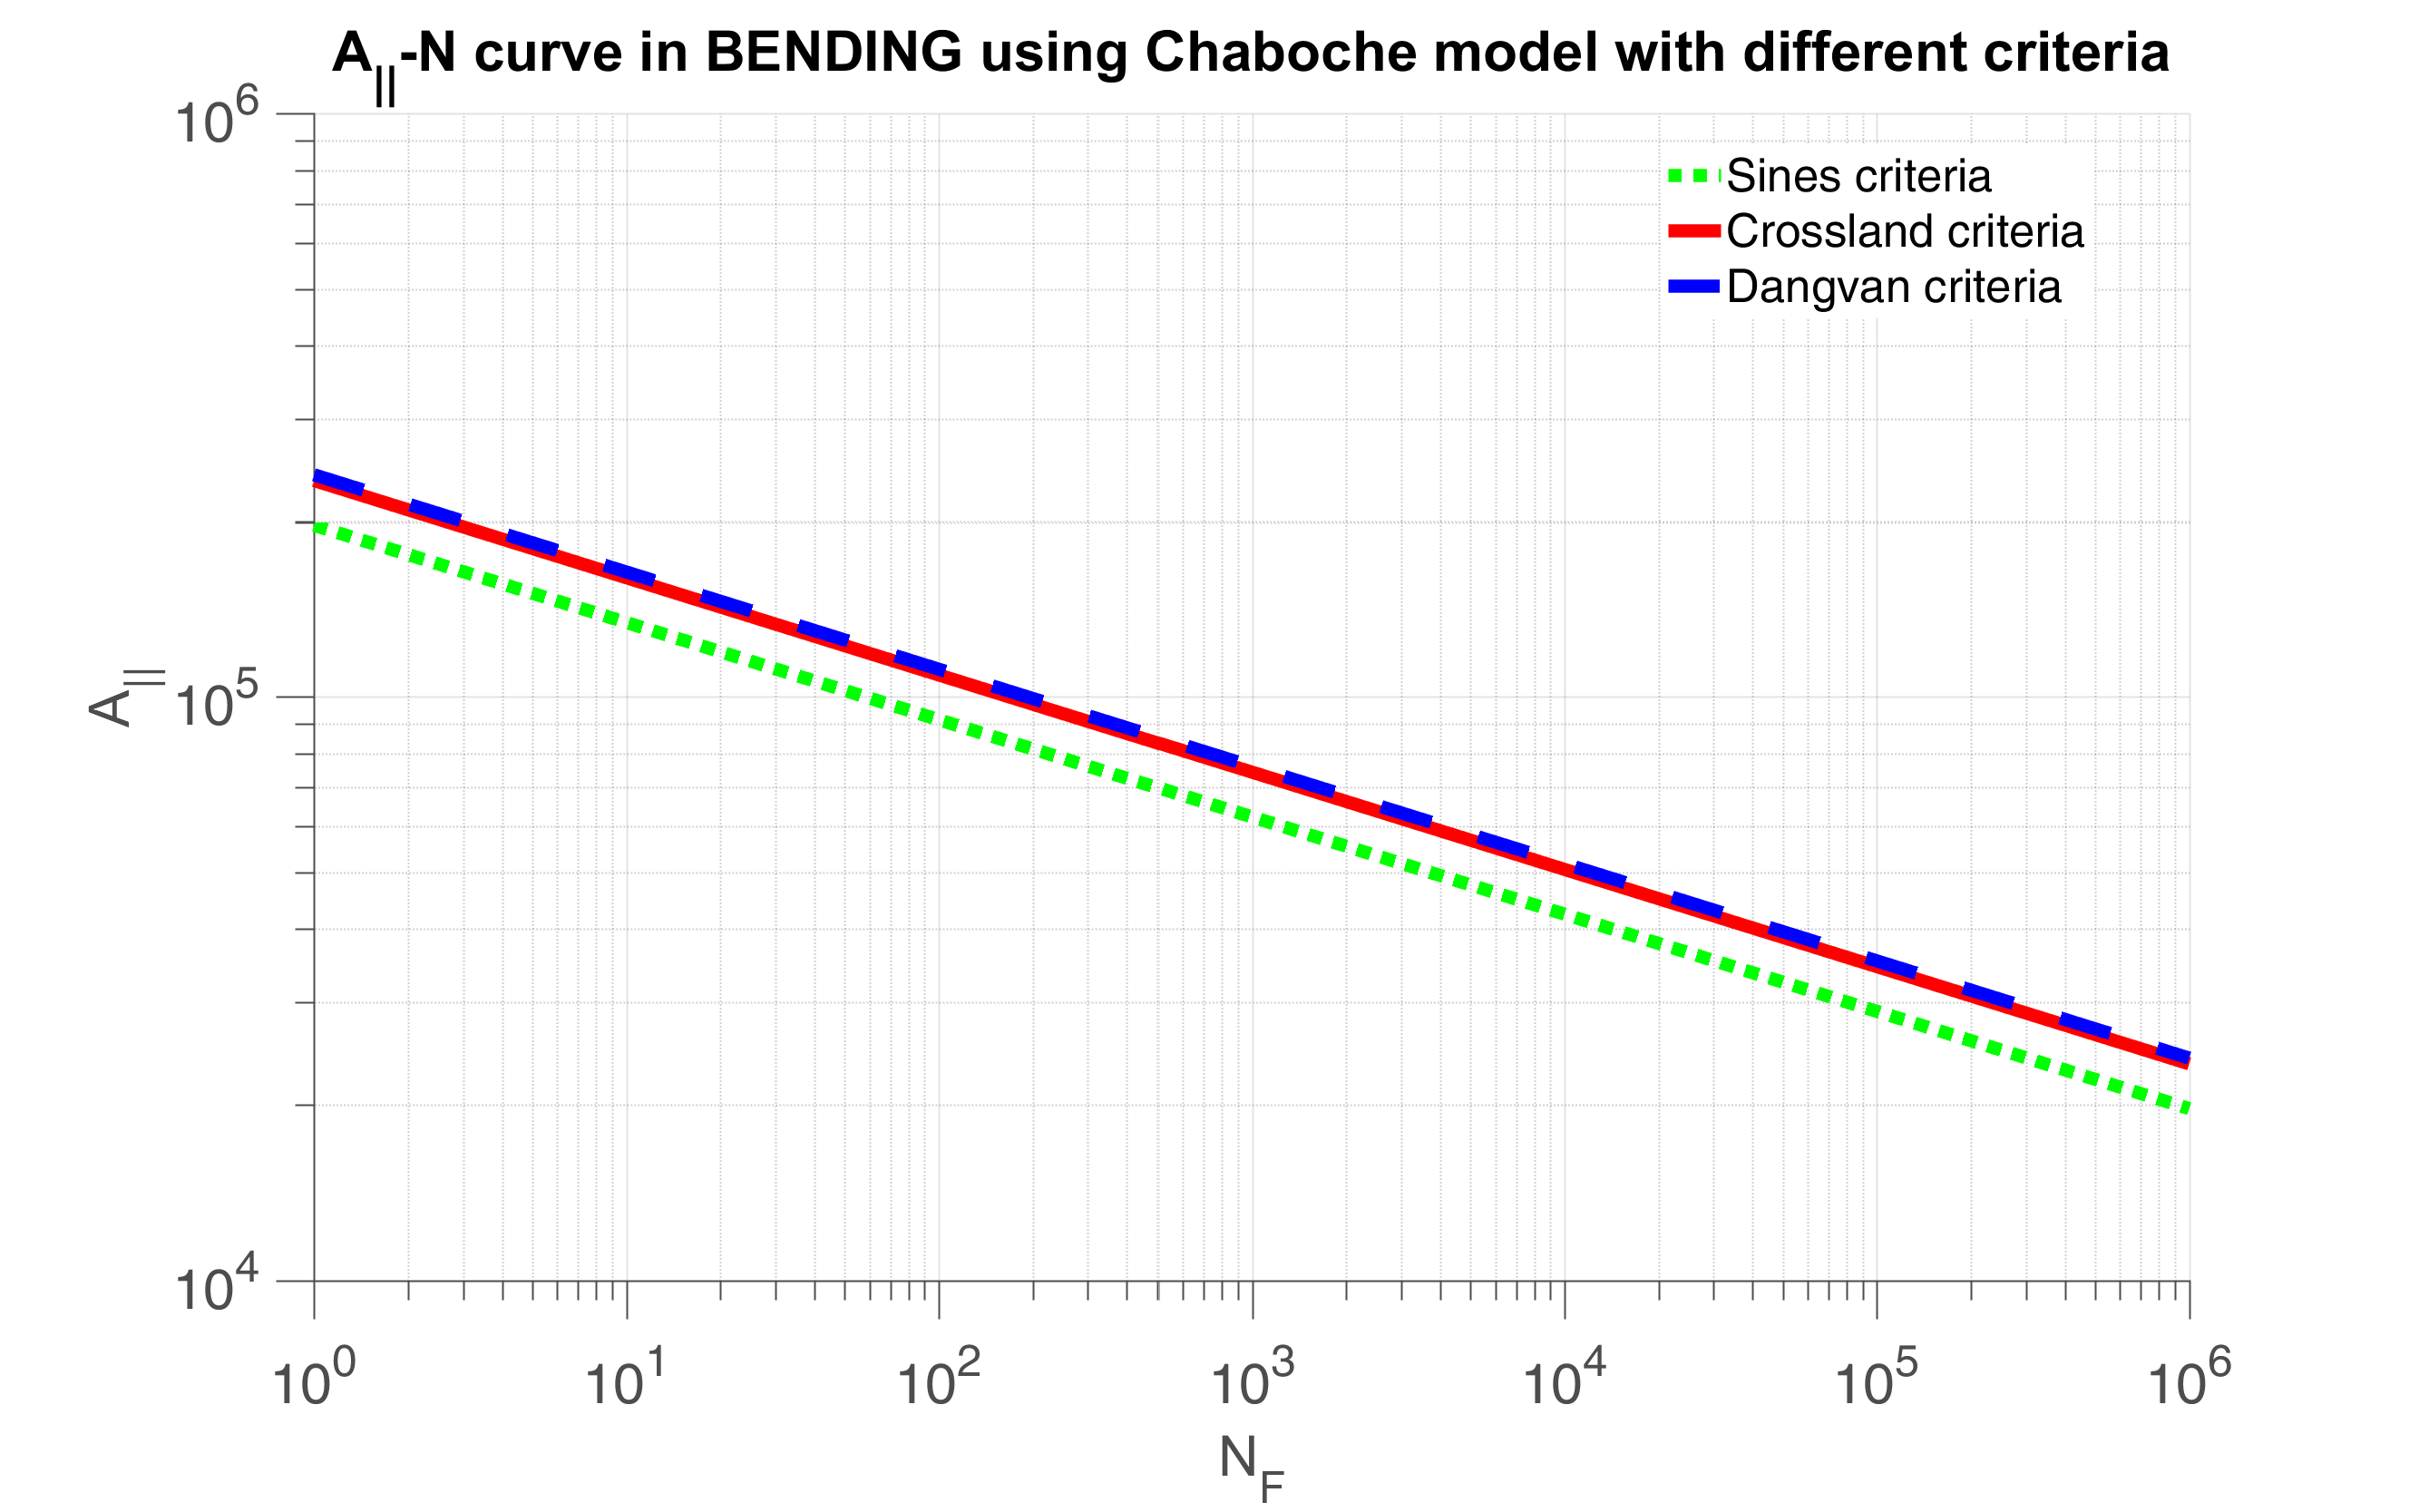
\includegraphics[width=\textwidth]{figures//JNbending.png} 
	\caption{$A_{\uppercase\expandafter{\romannumeral2}}-N_F$ curve in 4-point bending at y=3}
	\label{JNbending}
\end{figure}

In 4-point bending,we assume the first and second loading are respectively $F_1=1E6 N$ and $F_2=0.8E6 N$. 

\vspace{6pt}
$\sqrt{J_{2a_1}}=7.2194E5 Pa$

\vspace{6pt}
$\sqrt{J_{2a_2}}=5.7755E5 Pa$

\vspace{6pt}
$P_{m_1}=3.9298E5 Pa$

\vspace{6pt}
$P_{m_2}=3.1438E5 Pa$

Substituting the above to Eq.\eqref{eq.eta} we can get $\eta$ in High-Low sequence:
$$\eta_1=0.3174,$$

in Low-High sequence:
$$\eta_2=3.1510.$$

The predicted results are shown in \figref{2stressB}.

\begin{figure}[h!]
	\centering
	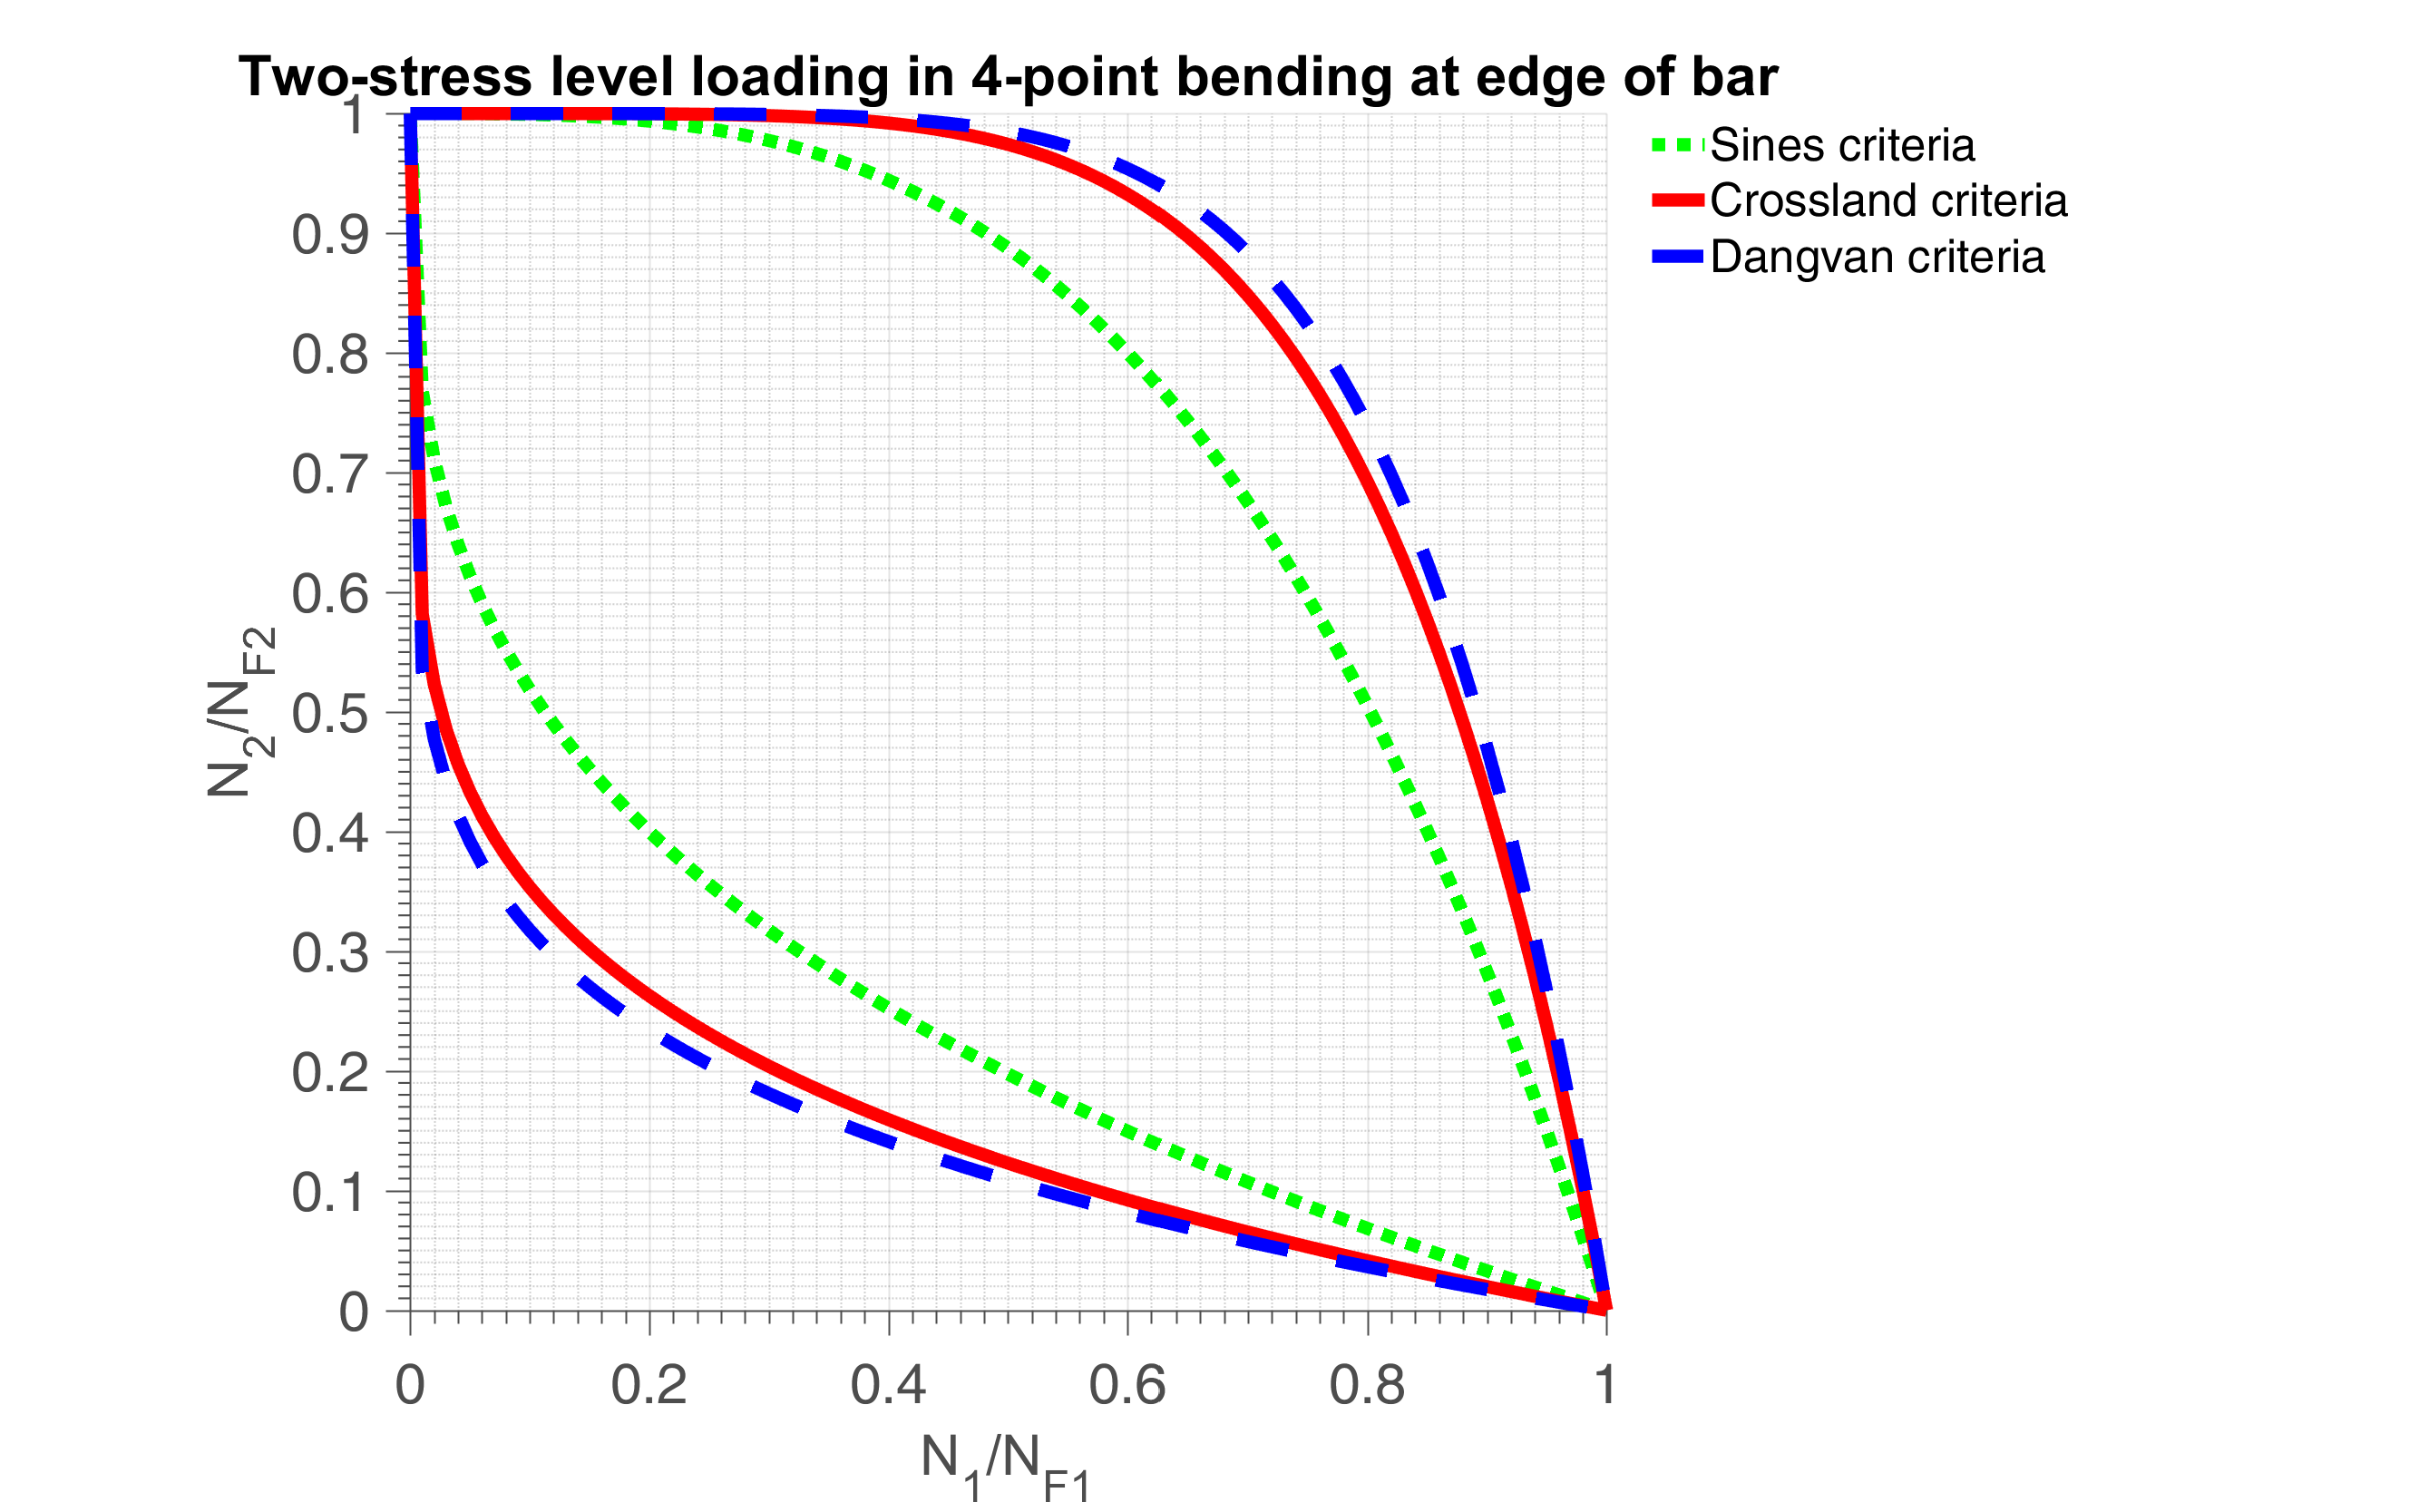
\includegraphics[width=\textwidth]{figures//2stressB.png} 
	\caption{Two-stress level loading in 4-point bending at y=3}
	\label{2stressB}
\end{figure}

\newpage
\subsubsection{Test on rotative bending}
From the fatigue zone we select $r=0.5$ as the radius to study. 
The $A_{\uppercase\expandafter{\romannumeral2}}-N_F$ figure is shown in \figref{JNRB}.

\begin{figure}[h!]
	\centering
	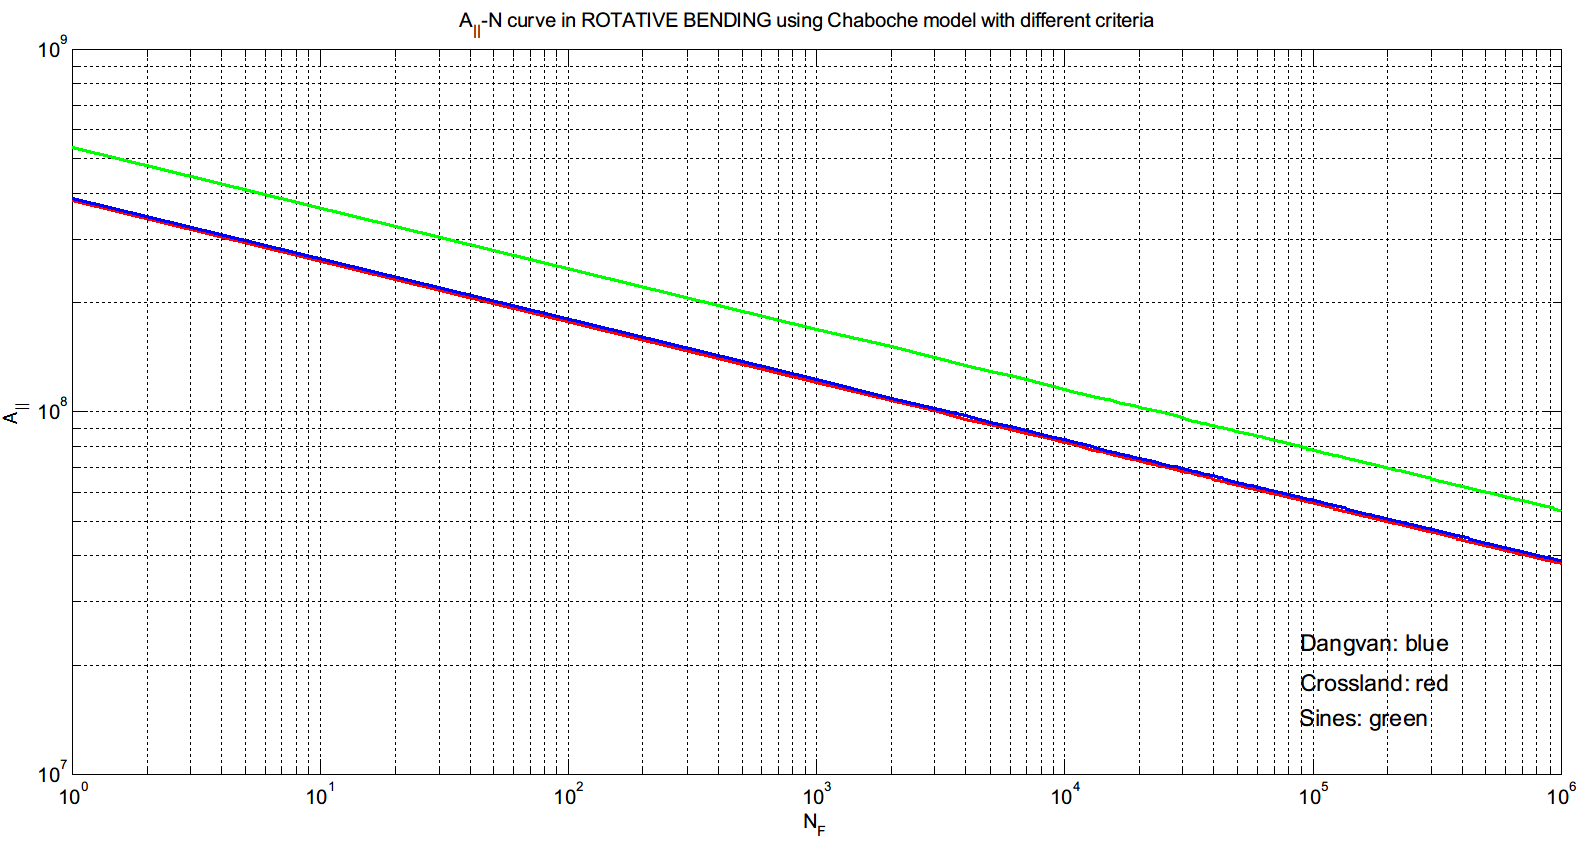
\includegraphics[width=\textwidth]{figures//JNRB.png} 
	\caption{$A_{\uppercase\expandafter{\romannumeral2}}-N_F$ curve in rotative bending at r=3}
	\label{JNRB}
\end{figure}

In rotative bending,we assume the rotating speed are $w=5rpm$. The applied force are respectively $F=9E5 N$ and $F=3E5 N$. We select:

$s_{-1}=f_{-1}=400MPa$, $\sigma_{u}=1000MPa$

\vspace{6pt}
$\sqrt{J_{2a_1}}=7.0226E8 Pa$

\vspace{6pt}
$\sqrt{J_{2a_2}}=6.6454E8 Pa$

\vspace{6pt}
$P_{m_1}=6.8921E8 Pa$

\vspace{6pt}
$P_{m_2}=7.1700E8 Pa$

Substituting the above to Eq.\eqref{eq.eta} we can get $\eta$ in High-Low sequence:
$$\eta_1=0.7170,$$

in Low-High sequence:
$$\eta_2=1.3947.$$

The predicted results are shown in \figref{2stressRB}.

\begin{figure}[h!]
	\centering
	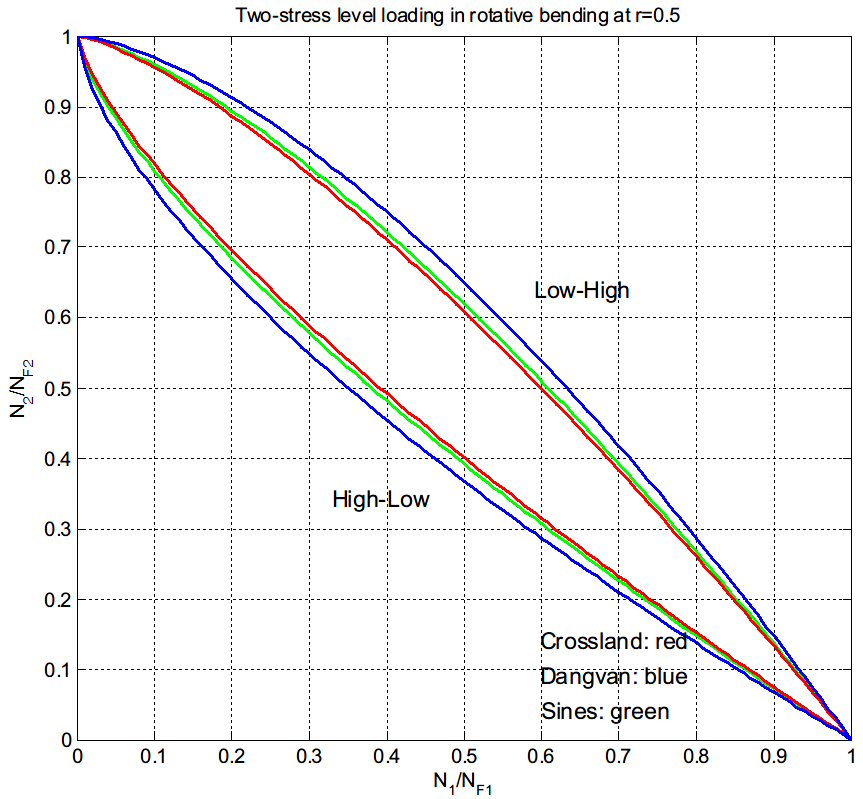
\includegraphics[width=\textwidth]{figures//2stressRB.png} 
	\caption{Two-stress level loading in rotative bending at r=0.5}
	\label{2stressRB}
\end{figure}
\clearpage


\section{Handling general loadings}

What makes automobile fatigue so difficult to predict is that, unlike standard tests done in a laboratory, an automobile's structure has to endure a complex, mostly random, set of static as well as cyclical stresses when in service, such as in \figref{complexloading} which could represent load data from testing or measurement, extracting the cyclic information can be challenging. 

\begin{figure}[h!]
	\centering
	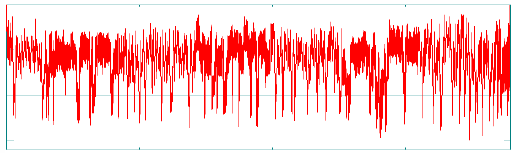
\includegraphics[width=\textwidth]{figures//complexloading.png} 
	\caption{Complex Cyclic Loading}
	\label{complexloading}
\end{figure}


\subsection{Cycle Counting Method}
A counting method is a method for identifying a statistical event
in a random loading sequence. This event can be, for example, extrema,
ranges or cycles of the signal. A method of counting stress cycles determines
therefore the number or the density of presence of the stress cycles in the loading signal.
In other words, the counting method consists in discretizing the loading sequence
variable in simple elementary cycles easy to implement in any forecasting process
of fatigue life. Indeed, each elementary cycle, extracted from the sequence of
load, is denoted by its amplitude and its mean value to which corresponds one
well-defined lifetime. Then, the elementary damage of the extracted cycle is calculated using
a rule of damage. The process repeats along the sequence studied to evaluate
the total damage by means of an accumulation law, and consequently to determine the number of
sequences at break.

Some methods of counting have been developed by the experts. They all lead to different results and therefore, for some, to errors in the calculation of the duration of life. We can cite by way of example six major families of counting techniques,
described in various works \cite{ASTM1985}:

\vspace{6pt}
\noindent
- the counting of the loading time,\\
- the counting of extrema between two passages by the mean value,\\
- the counting of areas,\\
- the counting of paired ranges,\\
- the counting of overflows,\\
- rainflow cycle counting, say ``the drop of water."
\vspace{6pt}

The object of all cycle counting methods is to compare the effect of variable amplitude load histories to fatigue data and curves obtained with simple constant amplitude load cycles. Rainflow counting is a process to obtain cyclic data of complex loading. Its name comes from the original description from the Japanese researchers Matsuiski and Endo where they describe the process in terms of rain falling off a pagoda style roof. A more insightful description based on cyclic plasticity is usually used to explain the method.

\begin{figure}[h!]
	\centering
	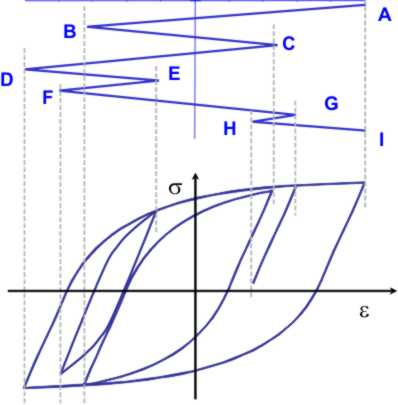
\includegraphics[width=0.4\textwidth]{figures//rainflow.jpg} 
	\caption{Complex Cyclic Loading}
	\label{rainflow}
\end{figure}

In \figref{rainflow} a simple loading history ( points A - I ) is plotted vertically so that it resembles a Japanese pagoda. The resulting deformation, stresses and strains, is plotted directly below the loading history. In the lower part of the figure, four cycles are easily identified. One large overall cycle, one intermediate cycle in the center of the plot, and two smaller cycles. Each cycle has its own strain range and mean stress. From a deformation viewpoint the process proceeds as follows. Start at A, the maximum strain, and unload the material to B. Then reload to point C and unload to D. When the material reaches the strain at point B during the unloading from C to D the material remembers its prior deformation and deforms along a path from A to D as if the event C-D never happened. This is better illustrated in the next part of the loading. Load from D to E and unload to F. Now load from F to G. When the material reaches the strain at point E during the loading from F to G the material remembers its prior deformation and deforms along a path from D to G as if the event E-F never happened. The same process occurs for G-H.

Rainflow counting will identify four cycles, A-D-I, B-C-B, E-F-E and G-H-G. Rainflow counting identifies the major load excursions, for example D to I, and treats subcycles like E-F and G-H as interruptions to the overall loading event D-I.

\vspace{6pt}
The five-step procedure to extract the cyclic data is summarized as follows:

1.  Determine the peaks and valleys of the stress/strain during cycling, and reorder to start from the absolute maximum (\figref{Reorder}).

2.  Visualize as draining water starting at the deepest valley (\figref{StressRange}).

3.  Measure total depth drained (stress range) and mean depth (mean stress), (\figref{StressRange}), and the number of these cycles in the load history.

4.  Continue by draining the next lowest (\figref{DrainWater}) and repeat until all valleys are drained. A  Rainflow  cycle is counted if the second segment is vertically shorter than the first and the third segments(i.e. 6-7 is smaller than 5-6 and 7-8).

5.  Use the damage rule to obtain the life from all cycles.

\begin{figure}[h!]
	\centering
	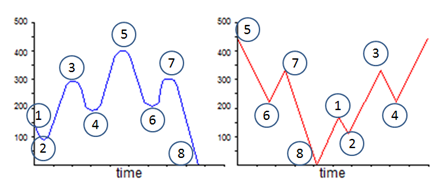
\includegraphics[width=0.6\textwidth]{figures//Reorder.png} 
	\caption{Reorder to Start from Absolute Maximum}
	\label{Reorder}
\end{figure}

\begin{figure}[h!]
	\centering
	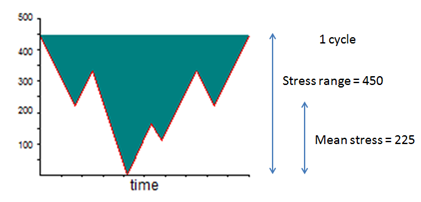
\includegraphics[width=0.6\textwidth]{figures//StressRange.png} 
	\caption{Imagine Filling with Water and Extract Stress Range and Mean Stress}
	\label{StressRange}
\end{figure}

\begin{figure}[h!]
	\centering
	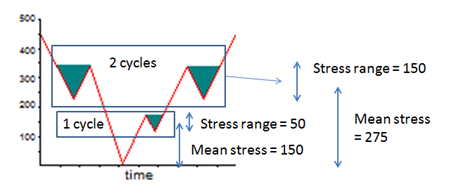
\includegraphics[width=0.6\textwidth]{figures//DrainWater.png} 
	\caption{Drain Water Starting at Lowest Valley and Repeat Cycle Extraction}
	\label{DrainWater}
\end{figure}   

\begin{figure}[h!]
	\centering
	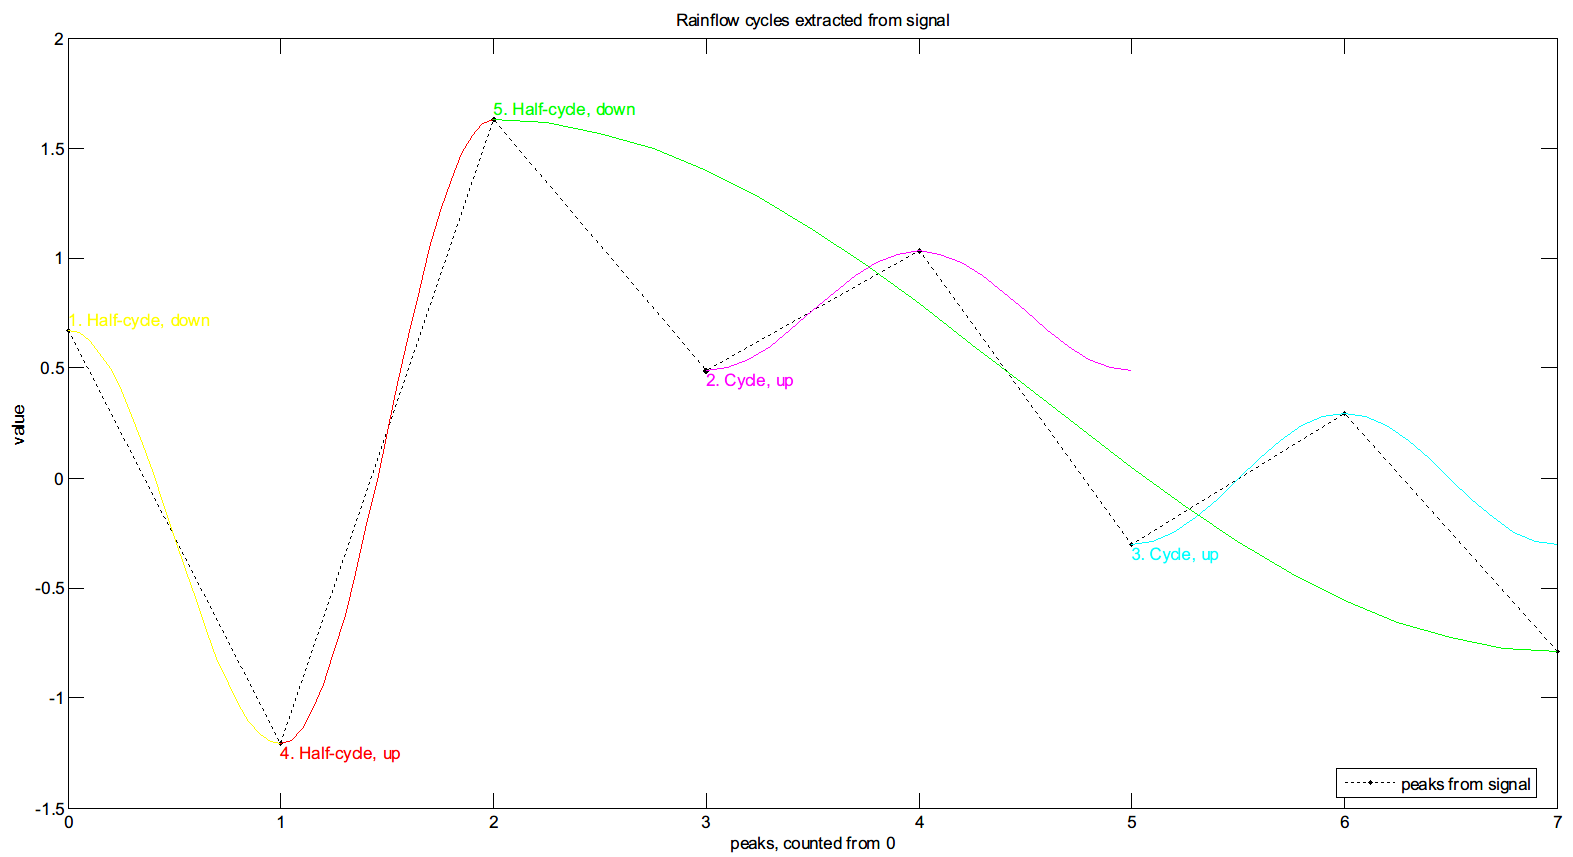
\includegraphics[width=\textwidth]{figures//rfdemo.png} 
	\caption{Rainflow counting method demonstration}
	\label{rfdemo}
\end{figure}  

Once all the cycles have been categorized, the Palmgren-Miner Rule is applied. Even though the linear damage rule ignores sequence effects, it is most widely used because of its simplicity and the fact that though many nonlinear damage models have been developed, unfortunately none can encompass many of the complicating factors encountered during complex variable amplitude loading. As an example, for this case assuming mean stress is ignored:

$$\sum_i \frac{N_i}{N_{F_i}}=\frac{1}{N_{F_{450}}}+\frac{1}{N_{F_{200}}}+\frac{1}{N_{F_{50}}}+...=1.$$

where n is replaced with the number of actual cycles of its corresponding type in the load history, for instance $N_{F_{450}}$ represents the life obtained from the $S-N$ data for a stress range of $450MPa$.  From this equation, the number of total cycles through the entire load history can be found.

The rainflow procedure can be automated so that cyclic content of complex loading can be extracted efficiently.  For example, fatigue computer codes such as $nCode DesignLife$ will accept files of test data, or the input of multiple load steps from a static or transient finite element analysis, and use the rainflow approach to automatically extract the cyclic data.  In addition, $DesignLife$ automates the Palmgrem-Miner Damage Rule calculation to determine number of cycles to failure, with the term cycle here defined as one pass through the entire time history. A computer program that accomplishes rainflow cycle counting applied to a complex history such as that in \figref{loadhistory} results in a table of ranges and means shown in \figref{loadhistory1}.

\begin{figure}[h!]
	\centering
	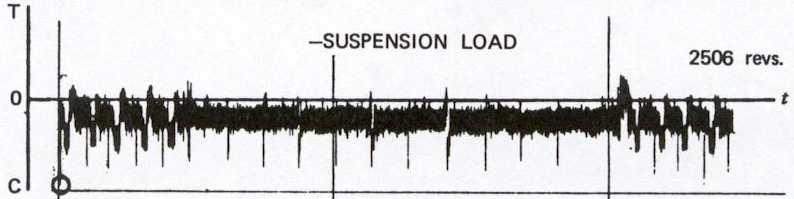
\includegraphics[width=0.9\textwidth]{figures//loadhistory.png} 
	\caption{Suspension load}
	\label{loadhistory}
\end{figure}

\begin{figure}[h!]
	\centering
	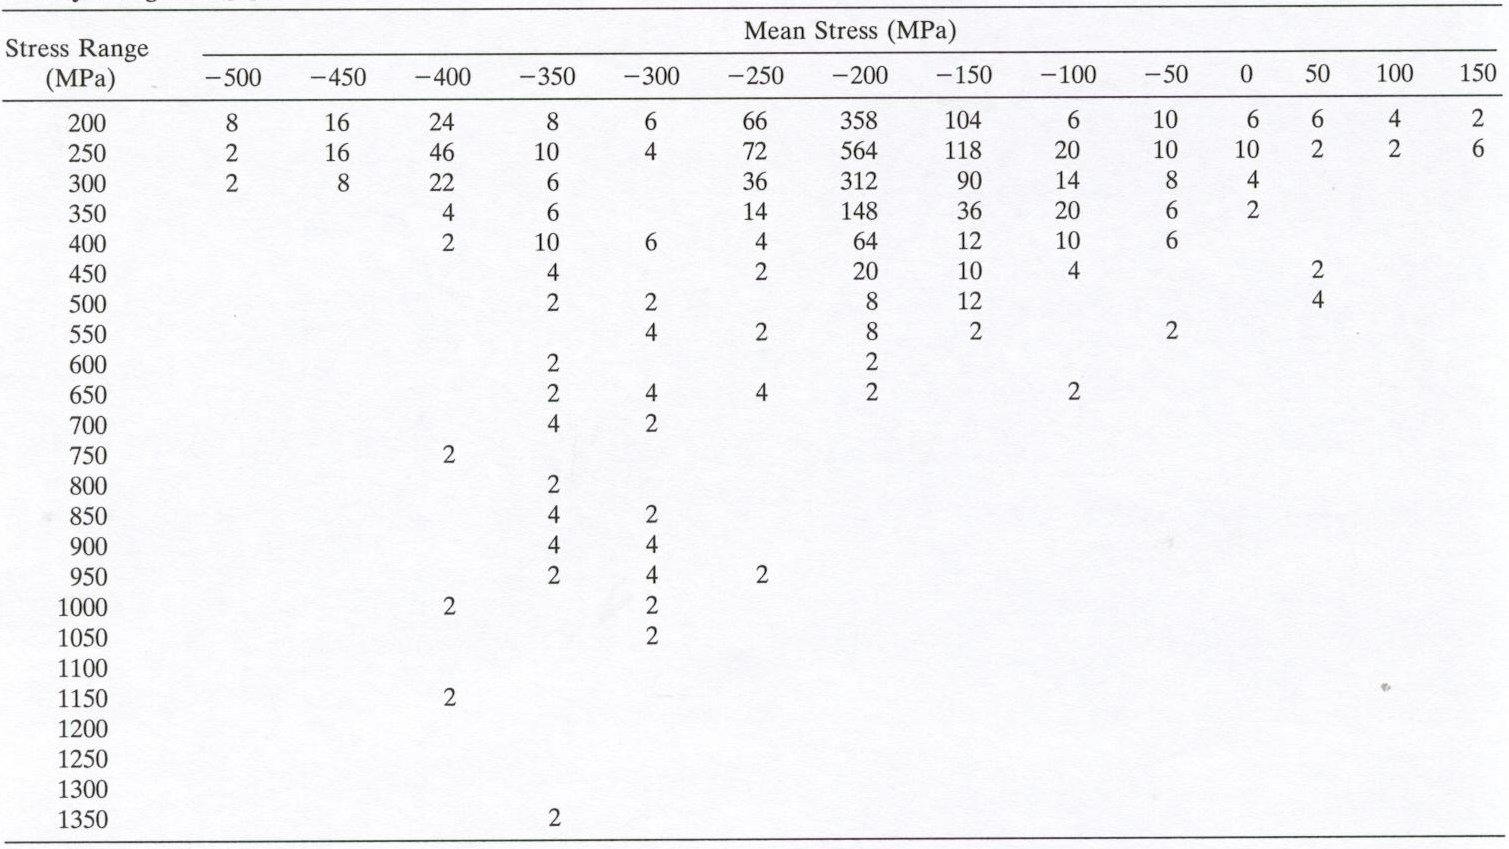
\includegraphics[width=\textwidth]{figures//loadhistory1.png} 
	\caption{Example of the Number of cycles at Various Stress Ranges and Mean Stress Combinations from the Suspension Load History in \figref{loadhistory}}
	\label{loadhistory1}
\end{figure}


\subsection{Multiaxial loading: existing models and limitations(Roux)}

In HCF, the material undergoes elastic deformation at the macroscopic level; plastic deformation occurs only near a stress concentration area, if there is.

\textbf{Discussion}

The Chaboche law is based on this assumption: fatigue damage occurs and accumulates only when the loading stress is higher than its fatigue limit. However, Eq.\eqref{chabochemulti} neglects the damage contribution of the loading stress which is lower than the fatigue
limit. According to some experimental results such as: Lu
and Zheng \cite{xi2008strengthening} \cite{xi2009strengthening} \cite{xi2009changes}, Sinclair \cite{sinclair1952investigation}, and Makajima et al. \cite{nakajima2007coaxing},
it has shown that the damage of low amplitude loads is one
of the main reasons for prediction errors. 

Impurities in the material affect the fatigue life. So does the material's hardness, and especially its surface condition. How the components were heat-treated in the factory is another factor. The operating temperature makes a difference, too. Worse still is the structural component's shape: notches and sharp corners create concentrations of stress that can initiate cracks. Thus further studies should be carried out concerning these factors.

\subsection{Multiscale energy dissipation approach}

The object of this work is to propose an energy based fatigue approach which takes into account impurities and hardness in the material which affect the fatigue life while handling multidimensional time varying loading histories.

Our fundamental thought is to assume that the local dissipated energy at small scale governs fatigue at failure. The proposal of our model is to consider a plastic behavior at the mesoscopic scale with a dependence of the yield function not only on the deviatoric part of the stress but also on the hydro static part. A kinematic hardening under the assumptions of associative plasticity is also considered. We follow the Dang Van paradigm. The structure is elastic at the macroscopic scale. At each material points, there is a stochastic distribution of weak points which will undergo strong plastic yielding, which contribute to energy dissipation without affecting the overall macroscopic stress.

Instead of using the number of cycles, we use the concept of loading time. To elaborate real life loading history more accurately, mean stress effect is taken into account in mesoscopic yield function and non-linear damage accumulation law are also considered in our model. Fatigue will then be determined from the plastic shakedown cycle and from a phenomenological fatigue law linking lifetime and accumulated mesoscopic plastic dissipation.
\subsection{Kinematic Hardening Models}
\subsubsection{Linear Kinematic Hardening}
A hardening rule is needed to
describe the behavior of the
material once it is plastically
deformed or yielded. One possible hardening rule is the
isotropic rule, which assumes
that strain hardening corresponds
to an enlargement of the yield
surface (i.e. an increase in  yield stress )
without change of shape or
position in the stress space. Another is the kinematic rule,
which assumes that strain
hardening shifts the yield surface
without changing its size or shape.
\begin{figure}[h!]
	\centering
	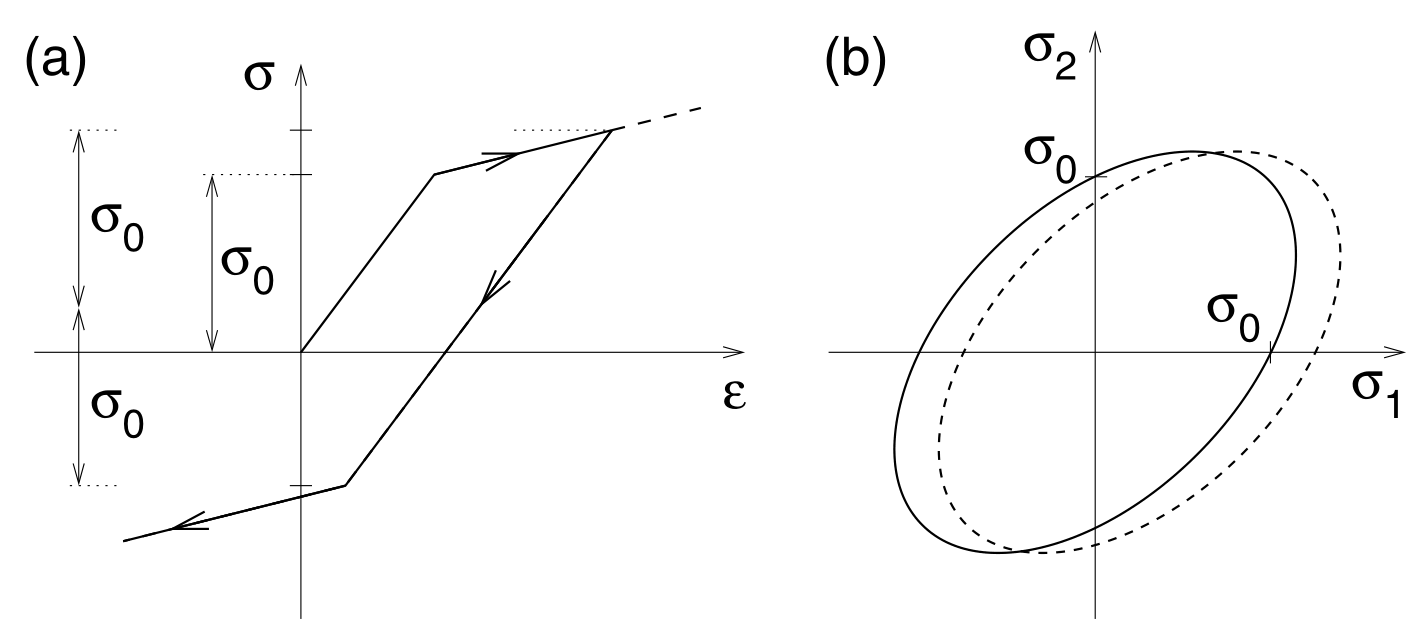
\includegraphics[width=0.8\textwidth]{figures//kinhard.png} 
	\caption{Kinematic hardening: a) uniaxial stress-strain diagram, b) evolution of the
		yield surface in the biaxial stress plane}
	\label{kinhard}
\end{figure}


Kinematic hardening rules are necessary,especially for the case of unloading and cyclic loading.In Kinematic Hardening the current loading surface is assumed not to expand but to move as a rigid body
within the stress space (\figref{kinhard}(b)). The use
of kinematic hardening is, for example, necessary to model the so-called Bauschinger
effect (Bauschinger, 1881). This effect is often observed in metals subjected to cyclic
loading. Even if the magnitudes of the yield stress in tension and in compression
are initially the same, this is no longer the case when the material is preloaded into
the plastic range and then unloaded. For example, after previous yielding in tension,
yielding in compression may start at a stress level lower than the initial yield stress
(\figref{kinhard}(a)).

Kinematic hardening leads to a translation of the loading surface, i.e. to a shift of
the origin of the initial yield surface. If the initial yield surface is described by a yield
function of the form
$$f(\sigma) = F(\sigma) -\sigma_0 $$
the shifted surface is obviously described by
$$f(\sigma,\sigma_b ) = F(\sigma-\sigma_b ) -\sigma_0$$
where $\sigma_b$ is the so-called backstress that represents the center of the shifted elastic
domain and plays the role of a tensorial hardening variable. Now we need a kinematic
hardening law that governs the evolution of the back stress. Melan (1938b) proposed
a law of the form
\begin{equation}
\sigma_b =\overline{H}_K \dot{\varepsilon}_p
\label{lineark}
\end{equation}
where $ \dot{\varepsilon}_p$ is the rate of effective plastic strain. According to which the rate of the back stress is proportional to the plastic strain rate. It is a macroscopic variable representing the
dislocation sub-structure resistance to deformation. 
The proportionality factor $\overline{H}_K$ is directly related to the plastic modulus and is derived from a simple
monotonic uniaxial curve.The linear hardening law Eq.\eqref{lineark} is often credited to Prager (1955, 1956); we will call it the Melan–Prager hardening rule. 

\subsubsection{Non-linear Kinematic Hardening}
%\begin{figure}[h!]
%		\includegraphics[width=\textwidth]{figures//kinehardening.gif} 
%		\caption{Dissipated energy in one cycle and number of cycles %to failure when $\beta=-1$}
%		\label{kinehardening}
%\end{figure}
To describe cyclic plasticity, one of the famous model is the non-linear kinematic hardening model formulated by Armstrong and Frederick. It is based on a physical mechanism of strain hardening and dynamic recovery and is capable of simulating the
multiaxial Bauschinger effect (movement of the yield surface in the stress space). Therefore, the model has been examined and implemented in commercial software and finite element analysis.

The Armstrong-Frederick model (AF) is a modification of the Melan–Prager linear kinematic hardening model. The only modification of this simple model is the "recal" term which changes the evolution law for the symmetric backstress tensor $\sigma_b$ from a classical linear kinematic hardening law (Melan–Prager) to a nonlinear kinematic hardening law. The term is proportional to the current back stress multiplied by the norm of the plastic strain rate. According to the Armstrong-Frederick rule, the evolution of the
back stress is governed by the differential equation:

\begin{equation}
\dot{\bm{\sigma}}_b=\underbrace{\overline{H}_K \dot{\varepsilon}_p}_{lin. kin. hardening} -\underbrace{\gamma\dot{p}\bm{\sigma}_b}_{recall - term, nonlinear hardening}
\label{nonlineark}
\end{equation}
where
$\dot{p}$ is the accumulated plastic strain rate given as $\sqrt{\dfrac{2}{3}}||\dot{\varepsilon}_p||$ . The constants
$\overline{H}_K$
and
$\gamma$
are determined from uniaxial tests.
At the onset of yielding, the
back stress is still zero and Eq.\eqref{nonlineark} gives the same response as the linear hardening
law Eq.\eqref{lineark}. As the back stress develops, the additional term becomes activated and
slows down the rate at which the back stress grows (i.e. reduces the tangent plastic
modulus).

\subsection{Weakening scales and yield function}
\subsubsection{The concept of weakening scales} 

We follow the Dan Van paradigm. The structure is elastic at the macroscopic scale. At each material points, there is a stochastic distribution of weak points which will undergo strong plastic yielding, without contributing to the overall macroscopic stress. From a microscopic point of view, there is a distribution of weakening scales, namely $s\in[1,\infty)$. Let $S_{max}$ be the macroscopic stress intensity at present time. Let $\sigma_y$ be the yield limit before weakening. Then we imagine that for a given scale $s$:

\vspace{6pt}
\noindent
$\bullet$ either $1\leqslant s\leqslant \sigma_y/S_{max}$, then $S_{max}\leqslant \sigma_y/s$, the material stays in the elastic regime and there is no energy dissipation at this scale.

\vspace{6pt}
\noindent
$\bullet$ or $\sigma_y/S_{max}\leqslant s\leqslant \infty$, then $S_{max}\geqslant \sigma_y/s$, the material is in the plastic regime and there is dissipated energy at scale $s$, contributing to the fatigue limit, which evolve through kinematic hardening.

In more details, at each scale $s$ of a plastic evolution process there is a weakened yield limit $\sigma_y/s$, zero initial plastic strain $\uline{\uline{\varepsilon}}_p$ and zero initial backstress $\uline{\uline{b}}$ at initial time $t_0$.


\vspace{6pt}

\subsubsection{Distribution of weakening scales}

We assume the weakening scales have a  probability distribution of power law: 
$$P(s) = Cs^{-\beta},$$

where $\beta$ is a material constant and $C$ is hardening constant. 
The choice of a power law has two reasons: on one hand, this type of distribution corresponds to a scale invariant process, on the other hand it leads in cyclic loading to a prediction of a number of cycles to life limit as a power law function of the stress intensity. More general laws can also be proposed.

The integrated probability ranging from macroscopic to microscopic stress  is unity. From this we can conclude:
$$\int_{1}^{\infty}P(s)ds=\left[ \frac{Cs^{1-\beta}}{1-\beta}\right] _{1}^{\infty}=0-\frac{C}{1-\beta}=1.$$


Then we know $C=\beta-1$, so the distribution is given by:
$$P(s) = Cs^{-\beta}=(\beta-1)s^{-\beta}$$ and it is shown in \figref{ps}.
\begin{figure}[!h]
	\centering
	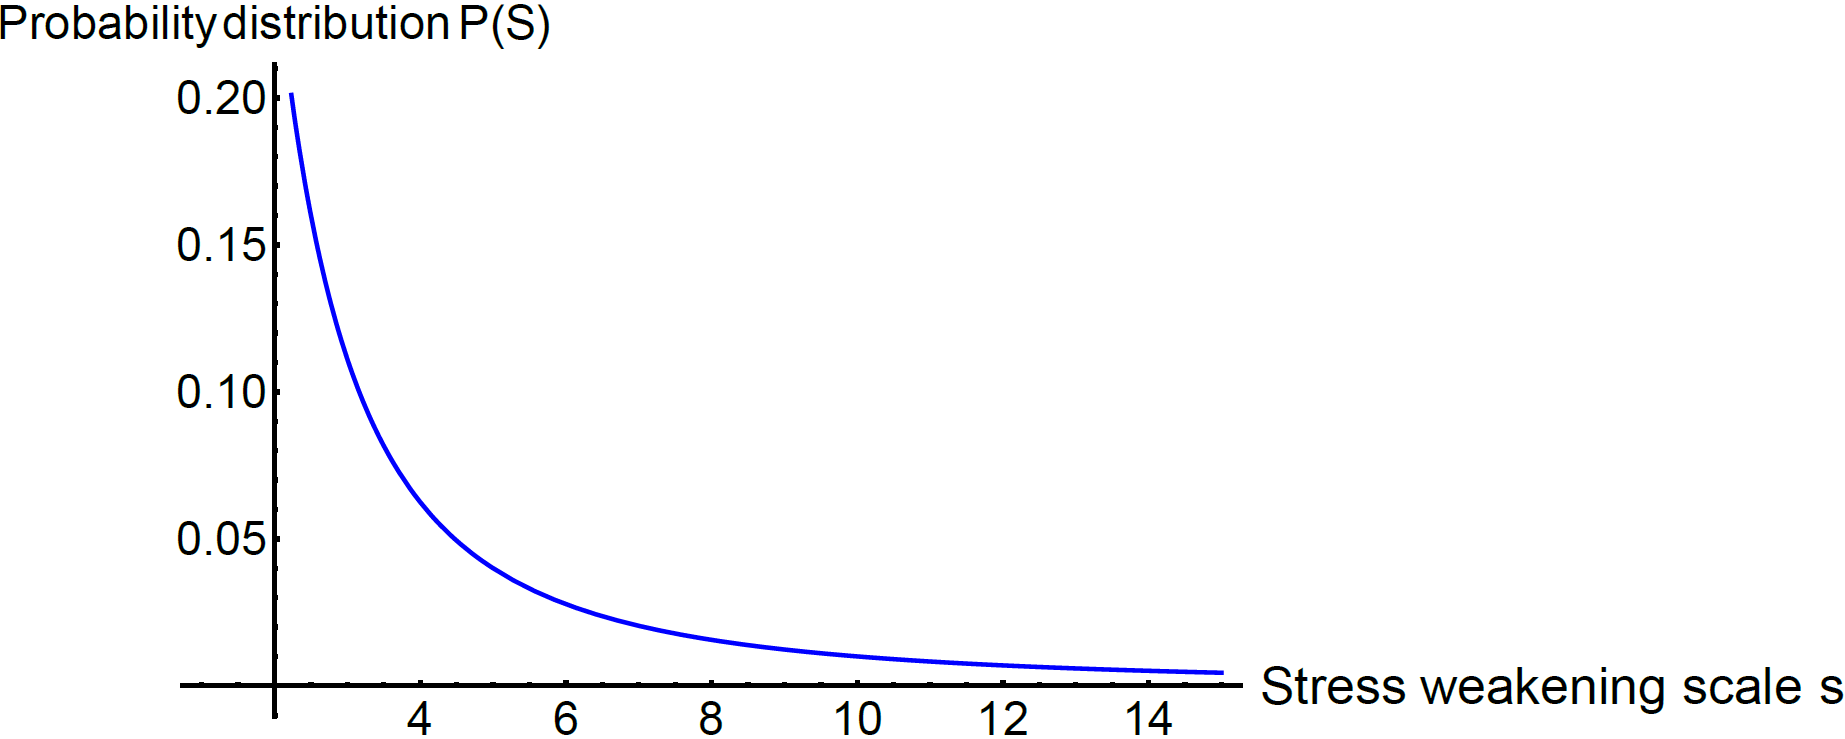
\includegraphics[width=0.9\textwidth]{figures//ps.png} 
	\caption{Weakening scales $s$ probability distribution curve}
	\label{ps}
\end{figure}


\subsubsection{Yield function with mean stress effect}

Positive mean stress clearly reduces the fatigue life of the material. In design evaluation of multiaxial fatigue with mean stress, a simplified, conservative relation between mean stress and equivalent alternating stress is necessary. We can improve the model by modifying the yield function $\sigma_y$ and the localization tensor.

\textbf{Christensen approach}
We can improve the model by modifying the yield function $\sigma_y$ and the localization tensor. There are several different models of yield function(Johnson Cook model if there is strain hardening, Christensen for mean stress effect), or we could integrate yield function with damage. Moreover, Sylvain Calloch at ENSTA Bretagne may have physical evidence and interpretation on the thermal dissipation in fatigue loading. 

The yield function that was given by Christensen\cite{christensen2000yield} integrates measures of damage, as well as intrinsic yield strength and concept of transitions. The derived yield function formalism resulted in the form as:

\begin{equation}
	\frac{\alpha K}{\sqrt{3}}\sigma_{kk}+\frac{(1+\alpha)^2}{2}s_{ij}s_{ij}\leqslant\frac{K^2}{(1+\alpha)},
	\label{eq:yieldfunc}
\end{equation}
where $\alpha$ changes the shape of the yield function, thus it is called the shape parameter. 
$$\alpha=\frac{\left| \sigma_{11}^C\right| }{\sigma_{11}^T}-1,$$
the new parameter $K$ is called the ideal or intrinsic strength which uniformly expands or contrasts the yield function, thus is is called the scale parameter:
$$K=\frac{(\sigma_{11}^C)^2}{\sqrt{3}\sigma_{11}^T}.$$
The intrinsic strength would occur if there were no damage or microstructure disturbance. 
$\sigma_{11}^C$ and $\sigma_{11}^T$ are respectively compressive and tensile yield stress in uniaxial states($\left| \sigma_{11}^C\right| \geqslant\sigma_{11}^T$, for ductile materials, $\frac{1}{2}\leqslant\dfrac{\left| \sigma_{11}^C\right| }{\sigma_{11}^T}\leqslant 1$). The yield stress in uniaxial and shear states are give by:

\begin{equation}
	\begin{split}
		&\sigma_{11}^C=\frac{-\sqrt{3}K}{(1+\alpha)}\\
		&\sigma_{12}^Y=\frac{K}{(1+\alpha)^{3/2}} \\
		&\sigma_{11}^T=\frac{\sqrt{3}K}{(1+\alpha)^2}.\\
	\end{split}
	\label{eq:uniyields}
\end{equation}

At $\alpha=0$, relations Eq.\eqref{eq:yieldfunc} and Eq.\eqref{eq:uniyields} show the behavior to be that of purely Mises type. This is taken to be the ideal condition where the intrinsic strength $K$ solely determines the yield strength. As the shape parameter increases beyond the value $\alpha=1$, the yield function behaves in accordance with  a state of increasing crack density or any other physical weakening. The term fracture, as used here for behavior at or near $\alpha=1$, actually corresponds to fracture mechanics for non-interacting cracks. Beyond this range near $\alpha=1$ or $\alpha\to\infty$ has simply been called yield or failure. Parameter $\alpha$ could be easily viewed as a damage measure or microstructure parameter since it represents microstructure changes on any scale that causes deviation from the ideal state. 

It is concluded a decrease in mean stress $\sigma_{kk}$ reduces the effective value of $\alpha$. That is, moving the behavior toward ductile case. Alternatively, increasing the mean stress moves $\alpha$ toward larger values, which is taken to be that of brittle behavior.

The fully expanded form of the yield function Eq.\eqref{eq:yieldfunc} is:
\begin{equation}
	\begin{split}
		&\frac{\alpha K}{\sqrt{3}}(\sigma_{11}+\sigma_{22}+\sigma_{33})\\
		+&(1+\alpha)^2\left[\frac{(\sigma_{11}-\sigma_{22})^2+(\sigma_{22}-\sigma_{33})^2+(\sigma_{33}-\sigma_{11})^2}{6}
		+(\sigma_{12}^2+\sigma_{23}^2+\sigma_{31}^2) \right]\\
		\leqslant&\frac{K^2}{(1+\alpha)}.\\
	\end{split}
\end{equation}

The most compact form of Eq.\eqref{eq:yieldfunc} is:
\begin{equation}
	\frac{1}{2}s_{ij}s_{ij}\leqslant\eta K^2,
\end{equation}
where $\eta$ is a nondimensional scaling factor on $K^2$, determined by mean normal stress.
$$\eta=\frac{1-\dfrac{\alpha(1+\alpha)}{\sqrt{3}K}\sigma_{kk}}{(1+\alpha)^3}<1$$


The mean stress $\sigma_{kk}$ has a positive relationship with the shape parameter $\alpha$. We suppose the material endures transition from ductile to brittle when $\alpha$ reaches 1. That means $\alpha$ has a very similar physical meaning with the damage parameter $D$.

\textbf{The Gerber parabola}
Several models are available
addressing the influence of tensile mean stress on fatigue life. Among these are the Gerber (Germany, 1874), Goodman
(England, 1899), and Soderberg (USA, 1930) models.  The modified Goodman criterion is often used as a design criterion
because it is more conservative than the Gerber criterion. The use of the Gerber criterion in the determination of member size is generally more computationally  intensive and so rather unattractive for many designers.

The effect of mean stress on the fatigue strength is commonly presented in Haigh diagrams as shown in \figref{haigh}, where $S_a / S_f$ is plotted against $S_m / S_u$. So is the fatigue strength at a given life under fully reversed ($S_m = 0$,$R = -1$) conditions. $S_u$ is the ultimate tensile strength. $S_f$ is the reversed fatigue strength. The data points thus represent combinations of $S_a$ and $S_m$ giving that life. The results were obtained for small unnotched specimens, tested at various tensile mean stresses. The straight lines are the modified Goodman and the Soderberg lines, and the curved line is the Gerber parabola. These are empirical relationships that are represented by the following equations:

\vspace{6pt}
Modified Goodman: $S_a/S_f + S_m/S_u = 1$

\vspace{6pt}
Gerber: $S_a/ S_f + (S_m/ S_u)^2 = 1$

\vspace{6pt}
Soderberg: $S_a/S_f+S_m/S_y=1$

\begin{figure}[h!]
	\centering
	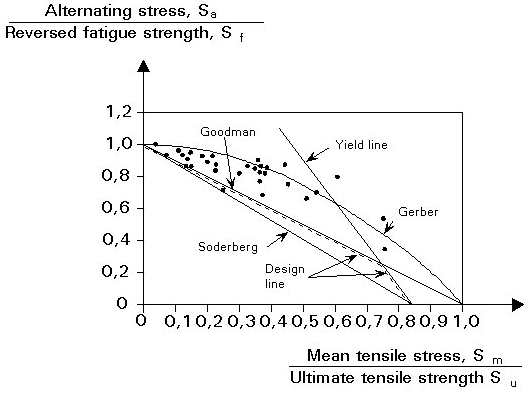
\includegraphics[width=0.8\textwidth]{figures//Gerber.png} 
	\caption{Haigh diagram showing test data points for the effect of mean stress, and the Gerber, modified Goodman and Soderberg relations.}
	\label{haigh}
\end{figure}


The idea is to consider as in Maitournam and Krebs\cite{Maitournam2011232} that the yield limit $\sigma_y$ can be reduced in presence of positive mean stress. The mesoscopic yield function can therefore be written as:
\begin{equation}
	f\left(s\right)=||\uline{\uline{S}}(s)-\uline{\uline{b}}(s)||+\left( \lambda \Sigma_H-\sigma_y\right) /s\leqslant 0
	\label{yieldfun}
\end{equation}
with $\uline{\uline{S}}$ denoting the deviatoric part of the stress tensor at microscale, and $\uline{\uline{b}}(s)$ the corresponding backstress at the same scale. The material remain in elastic regime when $f<0$ and in plastic regime when $f=0$.

\subsubsection{Local plastic model}
First we should describe the mesoscopic stress state.  The model considers a plastic 
behavior at the mesoscopic scale. The mesoscopic evolution equations are thus:

% \begin{numcases}{}
% 	\dot{\uline{\uline{S}}}(s,M,t)=dev\dot{\uline{\uline{\Sigma}}}(M,t)-\dfrac{E}{1+\nu}\dot{\uline{\uline{\varepsilon}}}^p(s,M,t), & Taylor-Lin scale transition model with unit localization tensor\cite{Bosia201239}.\\
% 	\dot{\uline{\uline{b}}}(s,M,t)=\dfrac{kE}{E-k} \dot{\uline{\uline{\varepsilon}}}^p(s,M,t) , & kinematic hardening model.\\
% 	\dot{\uline{\uline{\varepsilon}}}^p(s,M,t)=\gamma\dfrac{\partial f(s,M,t)}{\partial \uline{\uline{S}}}, & plastic flow rule assuming $\gamma=0$ when $f<0$ and  $\gamma\geqslant0$ when $f=0$.
% \end{numcases}

\begin{equation}
	\dot{\uline{\uline{S}}}(s,M,t)=dev\dot{\uline{\uline{\Sigma}}}(M,t)-\dfrac{E}{1+\nu}\dot{\uline{\uline{\varepsilon}}}^p(s,M,t), 
\end{equation}
which defines a Taylor-Lin scale transition model with unit localization tensor\cite{Bosia201239}.
\begin{equation}
	\dot{\uline{\uline{b}}}(s,M,t)=\dfrac{kE}{E-k} \dot{\uline{\uline{\varepsilon}}}^p(s,M,t), 
\end{equation}
which is our isotropic kinematic hardening model.
\begin{equation}
	\dot{\uline{\uline{\varepsilon}}}^p(s,M,t)=\gamma\dfrac{\partial f(s,M,t)}{\partial \uline{\uline{S}}}, 
\end{equation}
which is the associated plastic flow rule assuming $\gamma=0$ when $f<0$ and  $\gamma\geqslant0$ when $f=0$.

Here E denotes the Young's modulus and k the hardening parameter. The local dissipated energy rate per volume at weakening scales $s$  is given by the local entropy dissipation:
\begin{equation}
	\dot{w}(s,M,t)=(\uline{\uline{S}}-\uline{\uline{b}})(s,M,t):\uline{\uline{\dot{\varepsilon}}}^p(s,M,t).
	\label{dissipated}
\end{equation}


\subsubsection{Energy dissipation in shear cycle with mean stress}
\textbf{Calibration on 39NiCrMo3 steel}
Monotonic properties of the 39NiCrMo3 steel:

\noindent
Young modulus $E=206000 MPa$

\noindent
Tensile strength $\sigma_u=856 MPa$

\noindent
Tensile yield strength $\sigma_y=625 MPa$

\begin{table}[!h]
	\centering
	\caption{Torsion test results on the 39NiCrMo3 steel}
	\label{39NiCrMo3}
	\begin{tabular}{ll|ll|ll}
		\hline
		\multicolumn{2}{l|}{\textbf{\begin{tabular}[c]{@{}l@{}}$\tau_m=0$\end{tabular}}} & \multicolumn{2}{l|}{\textbf{\begin{tabular}[c]{@{}l@{}}$\tau_m=45MPa$\end{tabular}}} & \multicolumn{2}{l}{\textbf{\begin{tabular}[c]{@{}l@{}}$\tau_m=90MPa$\end{tabular}}} \\
		{\color[HTML]{333333} \textbf{$\tau_a$}}                 & \textbf{$N_f$}                 & {\color[HTML]{000000} \textbf{$\tau_a$}}                 & \textbf{$N_f$}                 & \textbf{$\tau_a$}                            & \textbf{$N_f$}                            \\ \hline
		{\color[HTML]{333333} 255}                              & 5,00E+06                      & 240                                                     & 5,00E+06                      & 240                                         & 5,00E+06                                 \\
		{\color[HTML]{333333} 255}                              & 5,00E+06                      & 255                                                     & 5,00E+06                      & 240                                         & 5,00E+06                                 \\
		{\color[HTML]{333333} 255}                              & 5,00E+06                      & 255                                                     & 5,00E+06                      & 240                                         & 5,00E+06                                 \\
		255                                                     & 5,00E+06                      & 255                                                     & 3,54E+06                      & 240                                         & 5,00E+06                                 \\
		255                                                     & 5,00E+06                      & 255                                                     & 5,00E+06                      & 255                                         & 2,29E+06                                 \\
		270                                                     & 2410000                       & 255                                                     & 5,00E+06                      & 255                                         & 5,00E+06                                 \\
		270                                                     & 1076000                       & 255                                                     & 5,00E+06                      & 255                                         & 2,53E+06                                 \\
		270                                                     & 1720000                       & 255                                                     & 5,00E+06                      & 255                                         & 2,95E+06                                 \\
		270                                                     & 1263000                       & 270                                                     & 2516000                       & 255                                         & 5,00E+06                                 \\
		270                                                     & 5,00E+06                      & 270                                                     & 1397000                       & 255                                         & 3,85E+06                                 \\
		270                                                     & 1,58E+06                      & 270                                                     & 7,24E+05                      & 255                                         & 3,21E+06                                 \\
		285                                                     & 697000                        & 270                                                     & 2,55E+06                      & 270                                         & 6,55E+05                                 \\
		285                                                     & 2,89E+05                      & 270                                                     & 2,05E+06                      & 270                                         & 1,06E+06                                 \\ \hline
	\end{tabular}
\end{table}
The results are plotted in \figref{torsionSN}. Collaborated parameters are shown in Table. \ref{mean39NiCrMo3}.
\begin{figure}[h!]
	\centering
	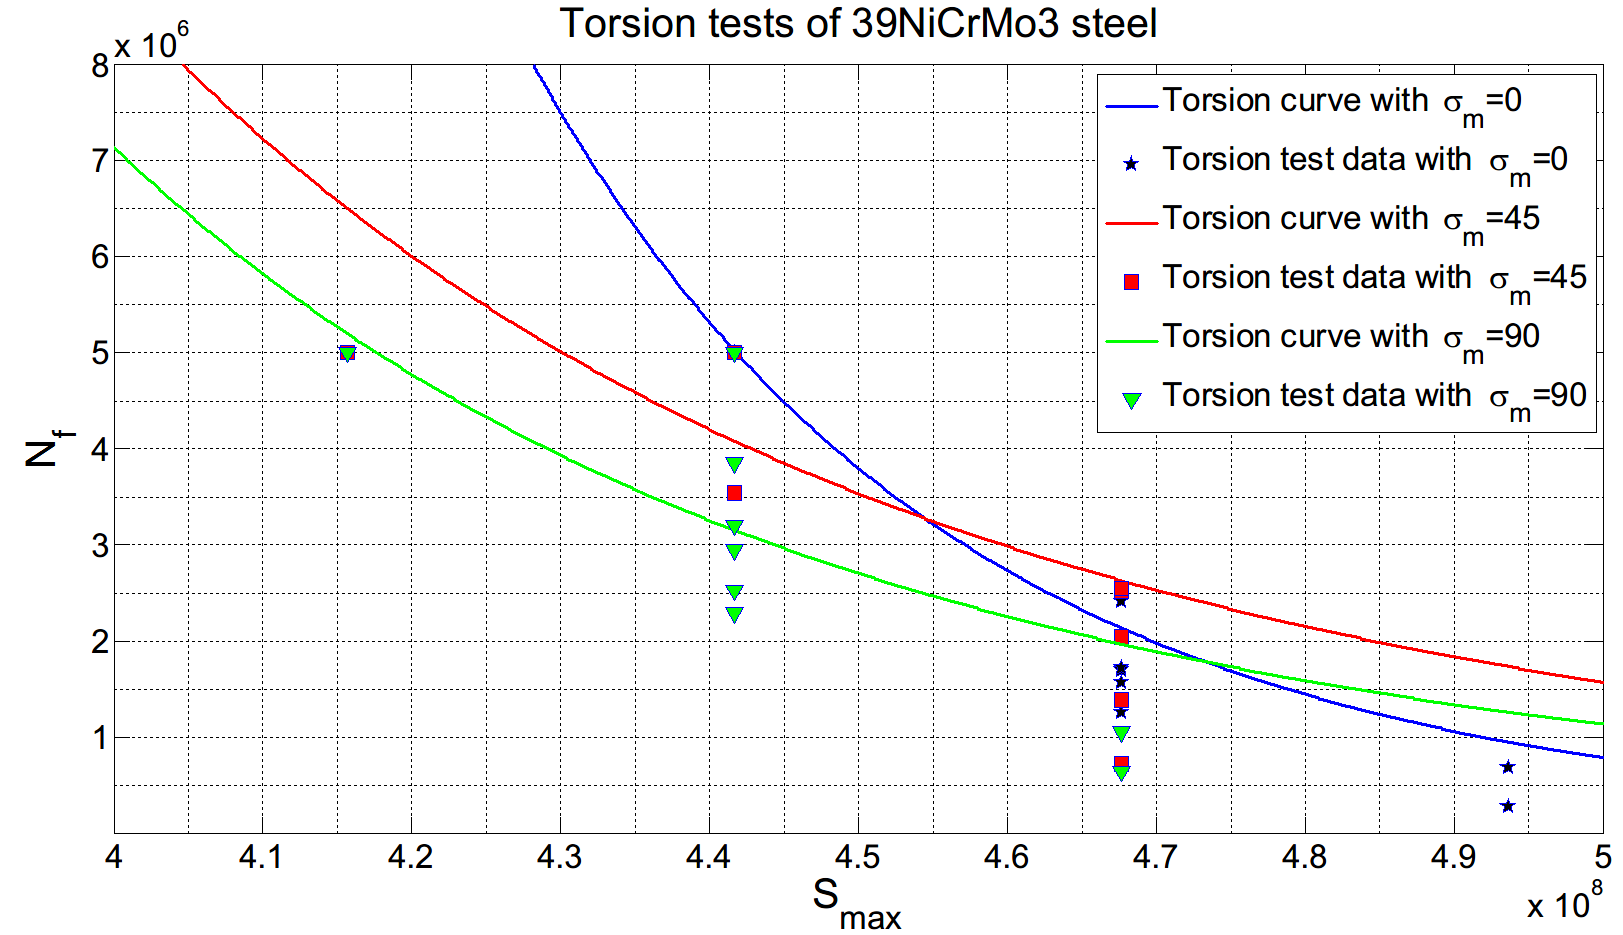
\includegraphics[width=0.9\textwidth]{figures//torsionSN.png} 
	\caption{Torsion test with mean stress}
	\label{torsionSN}
\end{figure}
\begin{table}[]
	\centering
	\caption{Parameter comparison of SM45C}
	\label{mean39NiCrMo3}
	\begin{tabular}{l|lllll}
		\hline
		& \textbf{Yield stress(MPa)} & \textbf{$W_F$}                  & \textbf{$\beta$} & \textbf{$k$} & \textbf{$\lambda$} \\ \hline
		\textbf{$\tau_m=0MPa$}                         & 625                        & 1.336E10                        & 13.92            & 0.3404       & 0                 \\
		{\color[HTML]{333333} \textbf{$\tau_m=45MPa$}} & 625                        & {\color[HTML]{000000} 5.102E11} & 6.671            & 0.506        & 1.734             \\
		{\color[HTML]{333333} \textbf{$\tau_m=90MPa$}} & 625                        & 4.907E12                        & 7.221            & 0.9293       & 3.003             \\ \hline
	\end{tabular}
\end{table}

\subsection{Construction of an energy based fatigue approach}

In a preliminary step, we will consider a simple macroscopic loading history $\uline{\uline{\Sigma}}(M, t)$ which is uniaxial
and time periodic of deviatoric amplitude $S_{max}$, and a Von Mises flow rule to see if we get a prediction of local failure for a number of cycles $N_F$ varying as $\Sigma^{-\beta}.$


\noindent
In uniaxial cyclic loading, there will be 3 kinds of loading patterns, as is shown in \figref{backstress}:

\vspace{6pt}
\begin{enumerate}
	
	\item	Elastic regime, in phase 2 and 4,where $\dot{\uline{\uline{\varepsilon}}}^p(s,M,t)=0$ ,  and $|\uline{\uline{S}}-\uline{\uline{b}}|<\left( \sigma_y-\lambda \Sigma_H\right)/s. $ 
	\vspace{6pt}
	
	\item Plastic regime according to plastic flow rule, with increasing plastic deformation, in phase 5 and 1, where	$\dot{\uline{\uline{\varepsilon}}}^p(s,M,t)=\gamma\dfrac{\uline{\uline{S}}(s)-\uline{\uline{b}}(s)}{||\uline{\uline{S}}(s)-\uline{\uline{b}}(s)||}> 0$ with  $\gamma=\left( dev\dot{\Sigma}\right)\left(\dfrac{kE}{E-k}+\dfrac{E}{1+\nu} \right) ^{-1}$ ,  with $\uline{\uline{S}}-\uline{\uline{b}}=\left( \sigma_y-\lambda \Sigma_H\right)/s$ and $\dot{\uline{\uline{S}}}-\dot{\uline{\uline{b}}}=0.$ 
	\vspace{6pt}
	
	\item Plastic regime in the other direction, in phase 3, there is	$\dot{\uline{\uline{\varepsilon}}}^p(s,M,t)<0$,  then $\uline{\uline{S}}-\uline{\uline{b}}=-\left( \sigma_y-\lambda \Sigma_H\right)/s$ and $\dot{\uline{\uline{S}}}-\dot{\uline{\uline{b}}}=0$ 
	
\end{enumerate}	

\begin{figure}[!h]
	\centering
	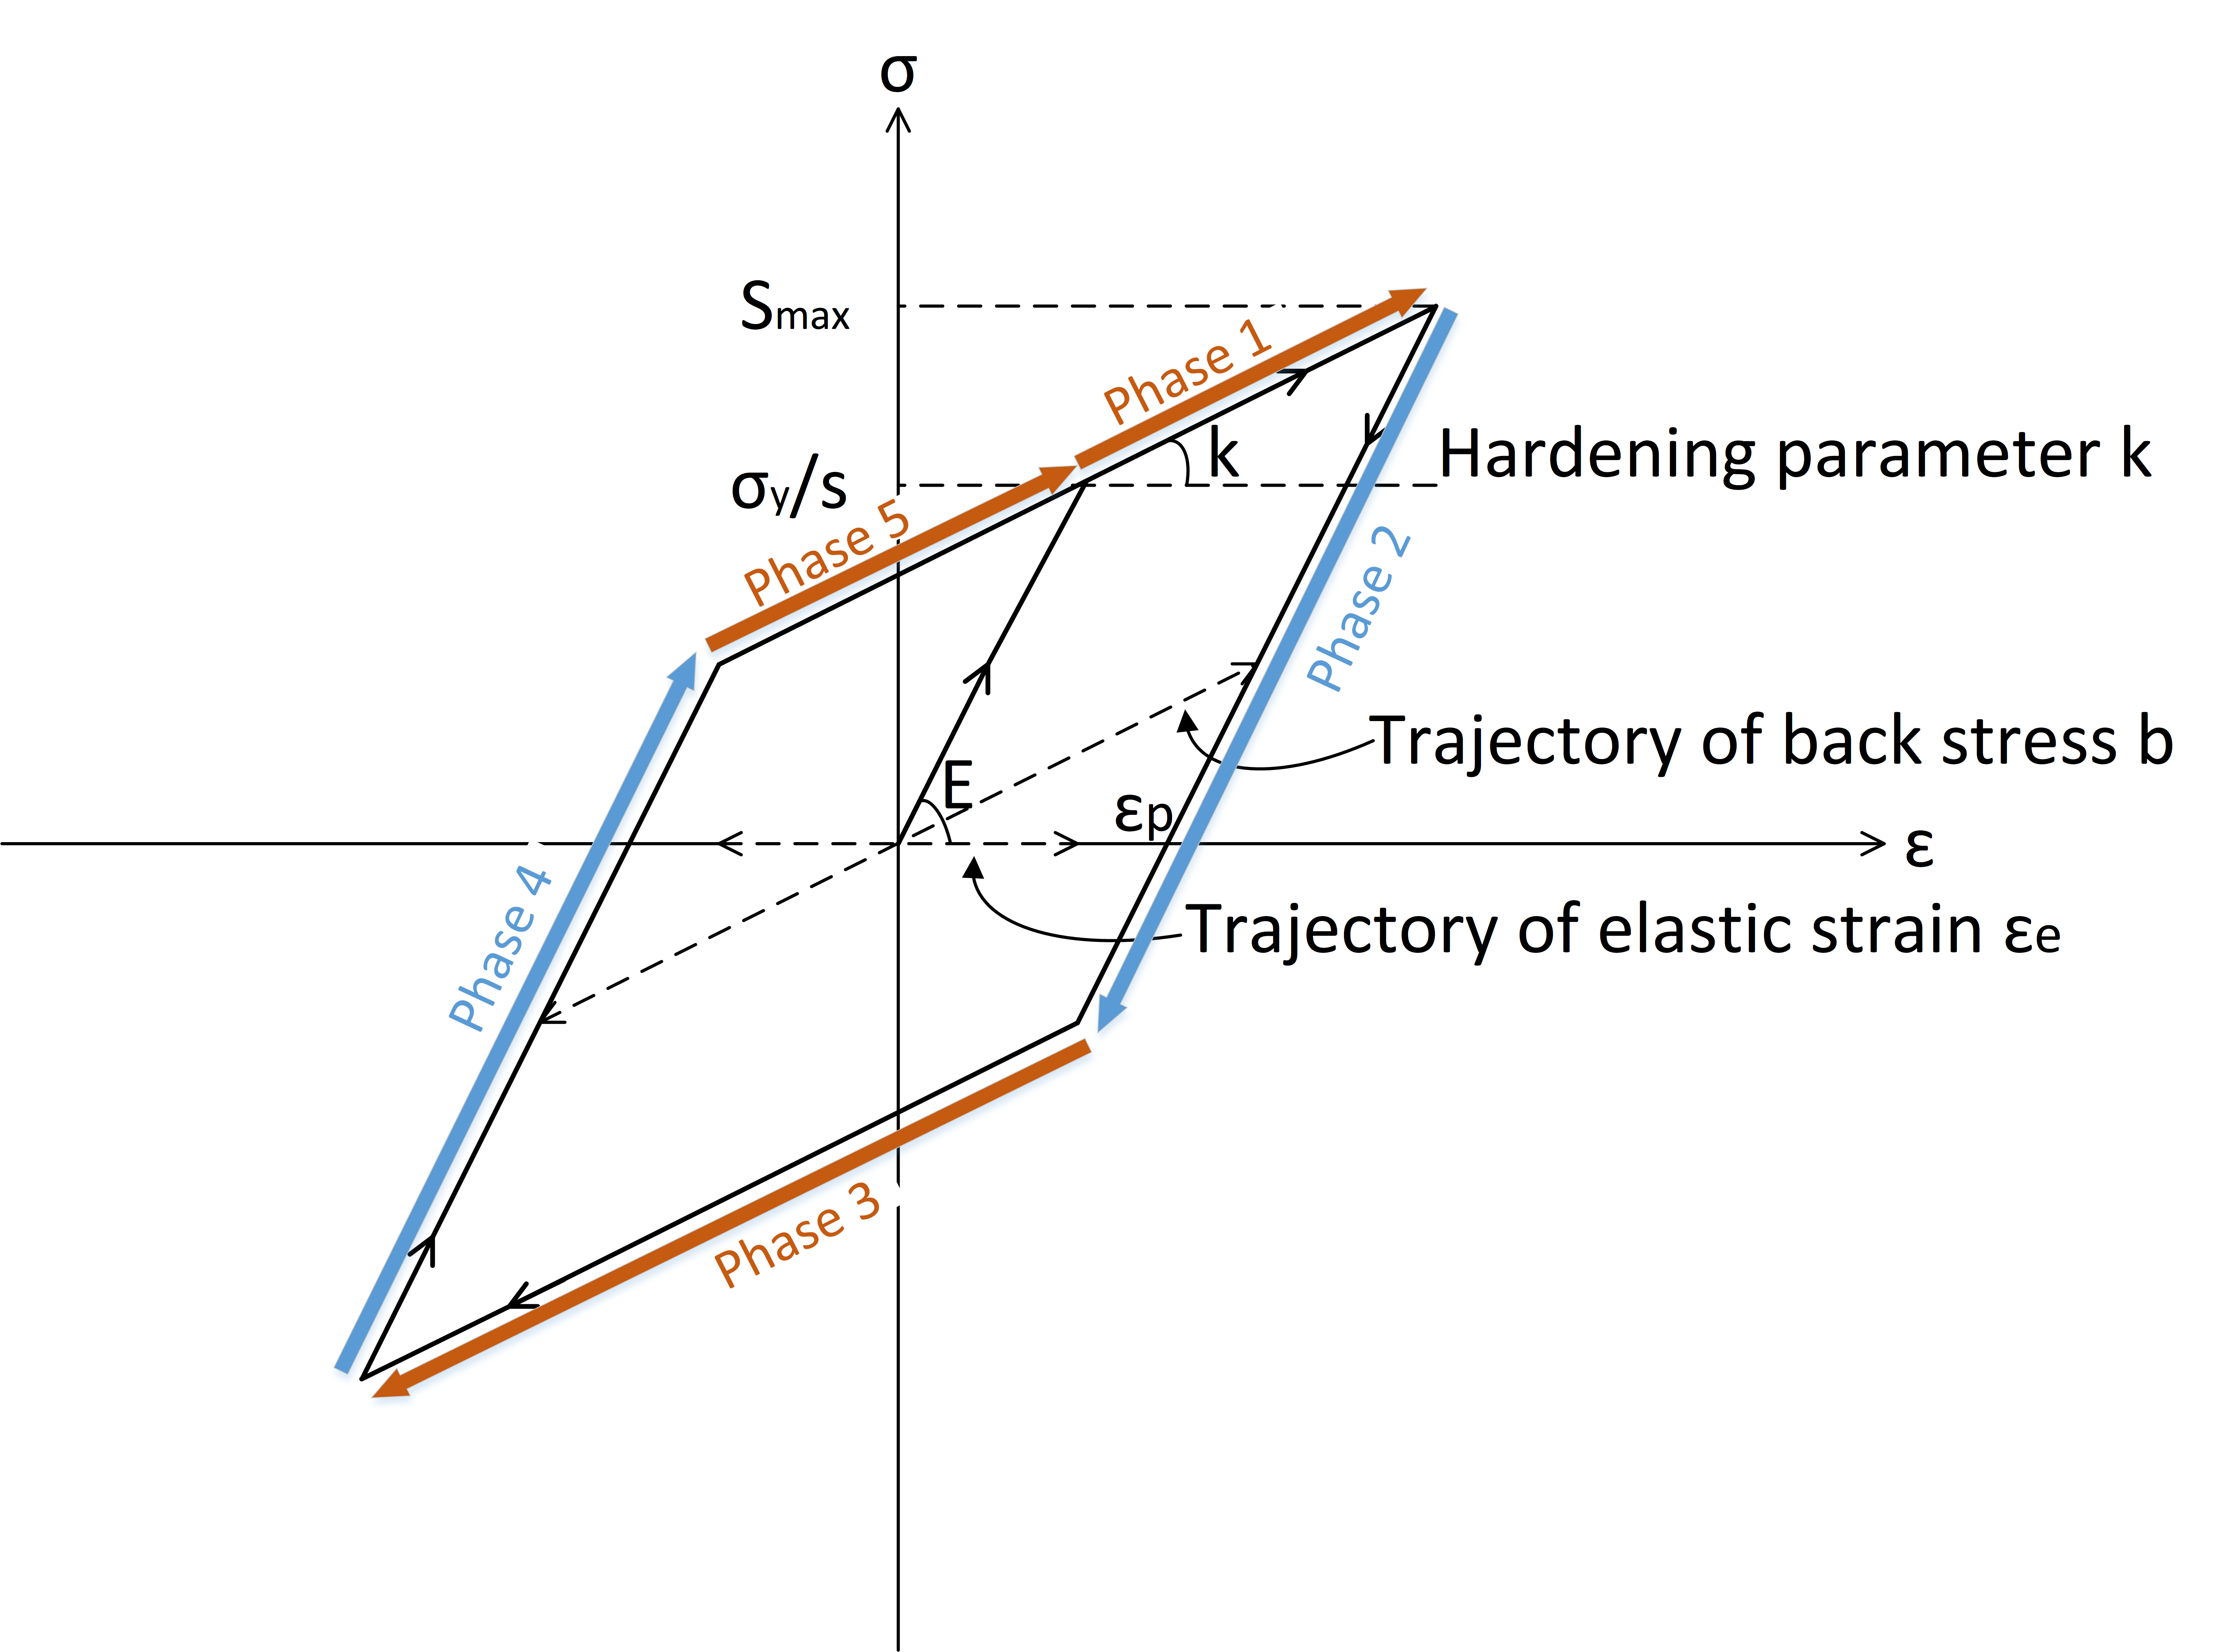
\includegraphics[width=0.9\textwidth]{figures//backstress.png} 
	\caption{Uniaxial load with plastic dissipation}
	\label{backstress}
\end{figure}


\noindent
\textbf{Phase 1:} The deviatoric stress amplitude increases from $\sigma_y/s$ to $S_{max}$.

\noindent
The material is in local plastic regime, then $\dot{\varepsilon}^p>0$ and $\dot{\sigma}-\dot{b}=0$ $\Rightarrow$ $\dot{\Sigma}-\dfrac{E}{1+\nu}\dot{\varepsilon}^p=\dfrac{kE}{E-k}\dot{\varepsilon}^p$ $\Rightarrow$ 
$$\dot{\varepsilon}^p=\dfrac{(E- k)(1+\nu)}{E(E+k\nu)}\dot{\Sigma}.$$

\vspace{6pt}
\noindent
$\Rightarrow$ $\dot{\varepsilon}^p$ varies from 0 to $\dfrac{(E- k)(1+\nu)(S_{max}-\sigma_y/s)}{E(E+k\nu)}$.

\vspace{6pt}
\noindent
From Taylor-Lin scale transition model:
$$\dot{\sigma}=\dot{\Sigma}-\dfrac{E}{1+\nu}\dot{\varepsilon}_p=\dot{\Sigma}-\dfrac{E-k}{E-\nu k}\dot{\Sigma}=\dfrac{k(1-\nu)}{E-k\nu}\dot{\Sigma}.$$

\vspace{6pt}
\noindent
$\Rightarrow$ $\sigma$ varies from $\sigma_y/s$ to $\sigma_y/s+\dfrac{k(1-\nu)(S_{max}-\sigma_y/s)}{E-k\nu}$.

\vspace{6pt}
$$\dot{b}=\dot{\Sigma}-\dfrac{E}{1+\nu}\dot{\varepsilon}_p=\dot{\Sigma}-\dfrac{E-k}{E-\nu k}\dot{\Sigma}=\dfrac{k(1-\nu)}{E-k\nu}\dot{\Sigma}.$$

\vspace{6pt}
\noindent
$\Rightarrow$ $b$ varies from $0$ to $\dfrac{k(1-\nu)(S_{max}-\sigma_y/s)}{E-k\nu}$.

\vspace{6pt}
\noindent
So the energy dissipation rate is: $$(\sigma-b)\dot{\varepsilon}^p=\dfrac{\sigma_y}{s}\dot{\varepsilon}^p=\dfrac{\sigma_y}{s}\dfrac{(E- k)(1+\nu)}{E(E+k\nu)}\dot{\Sigma}.$$

\noindent
The energy dissipation is: $$(\sigma-b)\Delta\varepsilon^p=\dfrac{\sigma_y}{s}\dfrac{(E- k)(1+\nu)(S_{max}-\sigma_y/s)}{E(E+k\nu)}.$$

\vspace{6pt}
\noindent
\textbf{Phase 2:} The deviatoric stress amplitude decreases from $S_{max}$ to $S_{max}-2\sigma_y/s$.

\noindent
The material is in local elastic regime, then $\dot{\varepsilon}^p=0$ and $\dot{\sigma}-\dot{b}=0$ $\Rightarrow$

\vspace{6pt}
\noindent
$\dot{b}=0$, $\dot{\sigma}=\dot{\Sigma}-\dfrac{E}{1+\nu}\dot{\varepsilon}_p=\dot{\Sigma}$.

\vspace{6pt}
\noindent
$\sigma$ varies from $\sigma_y/s+\dfrac{k(1-\nu)(S_{max}-\sigma_y/s)}{E-k\nu}$ to $-\sigma_y/s+\dfrac{k(1-\nu)(S_{max}-\sigma_y/s)}{E-k\nu}$.

\vspace{6pt}
\noindent
$\sigma-b$ varies from $\sigma_y/s$ to $-\sigma_y/s$.

\vspace{6pt}
\noindent
The energy dissipation rate is: $$(\sigma-b)\dot{\varepsilon}^p=0.$$

\vspace{6pt}
\noindent
\textbf{Phase 3:} The deviatoric stress amplitude decreases from $S_{max}-2\sigma_y/s$ to $-S_{max}$.

\noindent
The material is in local plastic regime, then $\dot{\varepsilon}^p>0$ and $\dot{\sigma}-\dot{b}=0$ $\Rightarrow$ 
$$\dot{\varepsilon}^p=\dfrac{(E- k)(1+\nu)}{E(E+k\nu)}\dot{\Sigma}$$ as opposite to phase 1 for $\dot{\Sigma}<0$.

\vspace{6pt}
\noindent
$\Rightarrow$ $\varepsilon^p$ varies from $\dfrac{(E- k)(1+\nu)(S_{max}-\sigma_y/s)}{E(E+k\nu)}$ to 

\noindent
$\dfrac{(E- k)(1+\nu)(S_{max}-\sigma_y/s-S_{max}-(S_{max}-2\sigma_y/s))}{E(E+k\nu)}=-\dfrac{(E- k)(1+\nu)(S_{max}-\sigma_y/s)}{E(E+k\nu)}$.

\vspace{6pt}
\noindent
From Taylor-Lin scale transition model:
$$\dot{\sigma}=\dot{\Sigma}-\dfrac{E}{1+\nu}\dot{\varepsilon}_p=\dot{\Sigma}-\dfrac{E-k}{E-\nu k}\dot{\Sigma}=\dfrac{k(1-\nu)}{E-k\nu}\dot{\Sigma}.$$

\vspace{6pt}
\noindent
$\Rightarrow$ $\sigma$ varies from $-\sigma_y/s+\dfrac{k(1-\nu)(S_{max}-\sigma_y/s)}{E-k\nu}$ to $-\sigma_y/s-\dfrac{k(1-\nu)(S_{max}-\sigma_y/s)}{E-k\nu}$.

\vspace{6pt}
$$\dot{b}=\dot{\Sigma}-\dfrac{E}{1+\nu}\dot{\varepsilon}_p=\dot{\Sigma}-\dfrac{E-k}{E-\nu k}\dot{\Sigma}=\dfrac{k(1-\nu)}{E-k\nu}\dot{\Sigma}.$$
\vspace{6pt}
\noindent
$\Rightarrow$ $b$ varies from $\dfrac{k(1-\nu)(S_{max}-\sigma_y/s)}{E-k\nu}$ to $-\dfrac{k(1-\nu)(S_{max}-\sigma_y/s)}{E-k\nu}$.

\vspace{6pt}
\noindent
So the energy dissipation rate is: $$(\sigma-b)\dot{\varepsilon}^p=-\dfrac{\sigma_y}{s}\dot{\varepsilon}^p=-\dfrac{\sigma_y}{s}\dfrac{(E- k)(1+\nu)}{E(E+k\nu)}\dot{\Sigma}.$$

\noindent
The energy dissipation is: $$(\sigma-b)\Delta\varepsilon^p=-\dfrac{\sigma_y}{s}\dfrac{(E- k)(1+\nu)(-2S_{max}+2\sigma_y/s)}{E(E+k\nu)}=\dfrac{2\sigma_y}{s}\dfrac{(E- k)(1+\nu)(S_{max}-\sigma_y/s)}{E(E+k\nu)}.$$



\vspace{6pt}
\noindent
\textbf{Phase 4:} The deviatoric stress amplitude increases from $-S_{max}$ to $-S_{max}+2\sigma_y/s$.

\noindent
The material is in local elastic regime, then $\dot{\varepsilon}^p=0$ and $\dot{\sigma}-\dot{b}=0$ $\Rightarrow$

\vspace{6pt}
\noindent
$\dot{b}=0$, $\dot{\sigma}=\dot{\Sigma}-\dfrac{E}{1+\nu}\dot{\varepsilon}_p=\dot{\Sigma}$.

\vspace{6pt}
\noindent
$\sigma$ varies from $-\sigma_y/s-\dfrac{k(1-\nu)(S_{max}-\sigma_y/s)}{E-k\nu}$ to $\sigma_y/s-\dfrac{k(1-\nu)(S_{max}-\sigma_y/s)}{E-k\nu}$.

\vspace{6pt}
\noindent
$\sigma-b$ varies from $-\sigma_y/s$ to $\sigma_y/s$.

\vspace{6pt}
\noindent
So the energy dissipation rate is: $$(\sigma-b)\dot{\varepsilon}^p=0.$$


\vspace{6pt}
\noindent
\textbf{Phase 5:} The deviatoric stress amplitude increases from $-S_{max}+2\sigma_y/s$ to $\sigma_y/s$.

\noindent
The material is in local plastic regime, then $\dot{\varepsilon}^p>0$ and $\dot{\sigma}-\dot{b}=0$ $\Rightarrow$ 
$$\dot{\varepsilon}^p=\dfrac{(E- k)(1+\nu)}{E(E+k\nu)}\dot{\Sigma}$$ as in phase 1.

\vspace{6pt}
\noindent
$\Rightarrow$ $\dot{\varepsilon}^p$ varies from $-\dfrac{(E- k)(1+\nu)(S_{max}-\sigma_y/s)}{E(E+k\nu)}$ to $0$.

\vspace{6pt}
$$\dot{\sigma}=\dot{\Sigma}-\dfrac{E}{1+\nu}\dot{\varepsilon}_p=\dot{\Sigma}-\dfrac{E-k}{E-\nu k}\dot{\Sigma}=\dfrac{k(1-\nu)}{E-k\nu}\dot{\Sigma}.$$

\vspace{6pt}
\noindent
$\Rightarrow$ $\sigma$ varies from $\sigma_y/s-\dfrac{k(1-\nu)(S_{max}-\sigma_y/s)}{E-k\nu}$ to $\sigma_y/s$.

\vspace{6pt}
$$\dot{b}=\dot{\Sigma}-\dfrac{E}{1+\nu}\dot{\varepsilon}_p=\dot{\Sigma}-\dfrac{E-k}{E-\nu k}\dot{\Sigma}=\dfrac{k(1-\nu)}{E-k\nu}\dot{\Sigma}.$$
\vspace{6pt}
\noindent
$\Rightarrow$ $b$ varies from $-\dfrac{k(1-\nu)(S_{max}-\sigma_y/s)}{E-k\nu}$ to $0$.

\vspace{6pt}
\noindent
So the energy dissipation rate is: $$(\sigma-b)\dot{\varepsilon}^p=\dfrac{\sigma_y}{s}\dot{\varepsilon}^p=\dfrac{\sigma_y}{s}\dfrac{(E- k)(1+\nu)}{E(E+k\nu)}\dot{\Sigma}.$$

\noindent
The energy dissipation is: $$(\sigma-b)\Delta\varepsilon^p=\dfrac{\sigma_y}{s}\dfrac{(E- k)(1+\nu)(S_{max}-\sigma_y/s)}{E(E+k\nu)}.$$


From the three phase analysis in local plastic regime, the dissipated energy is like $dW(phase1)=\dfrac{1}{2}dW(phase3)=dW(phase5)$ and the dissipation rate is like $d\dot{W}(phase1)=d\dot{W}(phase3)=d\dot{W}(phase5)$.
\begin{equation}d\dot{W}=\dfrac{(E-k)(1+\nu) }{E(E-k\nu)}\left( \dfrac{\sigma_y}{s}\right) \left| \dot{\Sigma}\right|   
\end{equation}

We can then calculate  the local dissipated energy $W$  at point $M$ during one cycle by cumulating the input of all sub-scales with their probabilities \cite{zepeng}.
\begin{equation}
	\begin{split}
		W_{cyc}&=4\int_{\left( \sigma_y-\lambda \Sigma_H\right) /S_{max}}^{\infty}dW(s,M,t)P(s)ds
		\\&=4\int_{\left( \sigma_y-\lambda \Sigma_H\right) /S_{max}}^{\infty}\dfrac{(E-k)(1+\nu) }{E(E+k\nu)}\dfrac{\sigma_y-\lambda \Sigma_H}{s}\left(S_{max}-\dfrac{\sigma_y-\lambda \Sigma_H}{s}\right)\left( \beta-1\right) s^{-\beta}ds
		\\&=\dfrac{4(E-k)(1+\nu)\left( \beta-1\right) }{ E(E+k\nu)\beta\left( \beta+1\right) }\dfrac{S_{max}^{\beta+1}}{\left( \sigma_y-\lambda \Sigma_H\right) ^{\beta-1}}.
	\end{split}
	\label{eq:w}
\end{equation}
If the dissipated energy accumulates linearly until a failure value $W_F$, we can get directly the time to failure from Eq.\eqref{lineartime}:
\begin{equation}
	T_{fail}=N_{F}t_{cyc}=\dfrac{W_F}{W_{cyc}}t_{cyc}=C(S_{max})^{-\beta-1}.
	\label{lineartime}
\end{equation}
From Eq.\eqref{eq:w}, we then obtain that the model predicts as expected a power law dependence in function of $S_{max}$.
However, experiments shows that the damage or the energy accumulation of a material evolves non-linearly in time. We should introduce below a method to handle such a nonlinearity.

\subsection{Damage accumulation without cycle counting}
\subsubsection{Energy approach with Chaboche law}
The Chaboche law\cite{lemaitre1990mechanics} is essentially a damage incremental law for cyclic loading of stress intensity $\sigma$ with a deviatoric part ${A}_{\uppercase\expandafter{\romannumeral2}}$ and hydrostatic part $\Sigma_H$, defining the damage increase by:

\begin{equation}\delta D = \left( 1 -(1-D)^{\gamma+1}\right)^\alpha \left(\frac{{A}_{\uppercase\expandafter{\romannumeral2}}/\left( 1-D\right) }{M(\Sigma_H)}\right)^\gamma \delta N
	\label{chabochemulti}
\end{equation} 
which writes equivalently as Eq.\eqref{integration}
\begin{equation}\delta [1-(1-D)^{\gamma+1}]^{1-\alpha}=(1-\alpha)(\gamma+1)\left(\dfrac{{A}_{\uppercase\expandafter{\romannumeral2}} }{M(\Sigma_H)}\right)^\gamma \delta N=\dfrac{\delta N}{N_F(\sigma)}.
	\label{integration}
\end{equation}
Here $N_F(\sigma)$ denotes the number of cycles at intensity $\sigma$ to failure as obtained by integration of Eq.\eqref{integration} from $D=0$ to $D=1$.

In our model, in case of a simple uniaxial cyclic loading, we propose to replace $\dfrac{1}{N_F(\sigma)}$ which is the relative unit increment of cycles by $\dfrac{W_{cyc}}{W_F}$, yielding the nonlinear damage incremental law:
\begin{equation}
	\delta[1-(1-D)^{\gamma+1}]^{1-\alpha}=\dfrac{W_{cyc}}{W_F}\delta N.
	\label{integrationW}
\end{equation}
This is a nonlinear law but used with a constant $\alpha$, there will be no sequence effect. In other words,
when applying two successive cycles of different intensities, the failure will occur at the same number of cycles whatever the order of the loading(high then low versus low then high).

\subsubsection{Generalized damage accumulation}
Formula \eqref{integration} is a general accumulation law which can be applied for any cyclic loading sequence provided that we can identify the multiscale value of the dissipated energy per cycle. 

But the notion of cycle itself may be hard to identify for general loadings. The idea is then to replace the relative increment of dissipated energy per cycle by the relative increment of dissipated energy per unit time, yielding:
\begin{equation}
	\delta [1-(1-D)^{\gamma+1}]^{1-\alpha}=\dfrac{\dot{W}}{W_F}\delta t.
	\label{dt}
\end{equation}

In a general loading case, $\dot{W}$ is to be computed. By integrating Eq.\eqref{dissipated} over all microscales, we get:
\begin{equation}\dot{W}(M,t)=\int_{s=1}^{\infty}\dot{w}(s,M,t)P(s)ds=\int_{s=1}^{\infty}\left(\uline{\uline{S}}-\uline{\uline{b}} \right) (s,M,t):\uline{\uline{\dot{\varepsilon}^p}}(s,M,t)P(s)ds.\label{Wdot}
\end{equation}
The evolution of $\uline{\uline{S}}$, $\uline{\uline{b}}$ and $\uline{\uline{\dot{\varepsilon}^p}}$ are given in section 1.4. Equation \eqref{dt} and \eqref{Wdot} are therefore our proposed damage law.

\section{Numerical implementation and validation}
\subsection{Integration rules for $\dot{W}$ and $\delta D$}
Our first approach takes one cycle as unit time. We compute analytically the energy dissipation at each scale during this cycle. The method is valid for simple loading history and which includes the integration on all weakening scales. The damage $D$ is accumulated after each cycle.

However, there are certain limitations of this method. Firstly we need a load history decomposition in cycles. Secondly in real life the perfect close loop cycle is hardly applicable.

Thus we propose in Eq.\eqref{dt} a more general method which can be integrated by a step by step strategy. We compute numerically the dissipation at different scales using an implicit Euler time integration of the constitutive laws of section 1.4. After which we make a numerical integration on different scales. Then we can update the damage and go to next time step. 

Instead of doing the scale integration directly which can be difficult for complex loading, the Gaussian Quadrature rule with Legendre points is used to give the value of local dissipated energy rate.

To use the Gaussian quadrature rule the limit range of integral must be from $-1$ to $1$, while the total dissipated energy  is expressed by integrating all the weakening scale $s$ ranging from 1 to infinity with their occurrence probabilities:
$$\dot{W}=\int_{1}^{\infty}\dot{w}(s) (\beta-1)(s)^{-\beta}ds.$$

\noindent
To change the limit range of integral from $[1,\infty]$ to $[1,0]$ we take as new integration variable
$u(s)= s^{-p}$ with $p=\beta-1$, yielding $u(1)=1$ and  $u(\infty)=0$ with
$$du=-ps^{-p-1}ds$$ 
that is
$$du=(-\beta+1) s^{-\beta}ds=(-\beta+1)s^{-\beta} ds.$$
Therefore the dissipated energy summed on all scales is:
\begin{equation}
	\begin{split}
		\dot{W}&=\int_{1}^{\infty}\dot{w}(s) (\beta-1)(s)^{-\beta}ds
		\\&=\int_{1}^{0}\dot{w}\left( u^{\frac{1}{1-\beta}}\right) (\beta-1) \frac{1}{-\beta+1}du
		\\&=\int_{0}^{1}\dot{w}\left( u^{\frac{1}{1-\beta}}\right) (\beta-1) \frac{1}{\beta-1}du
		\\&=\int_{0}^{1}\dot{w}\left( u^{\frac{1}{1-\beta}}\right)du
		\\&=\frac{1}{2}\int_{-1}^{1}\dot{w}\left[  \left( \frac{x+1}{2}\right) ^{\frac{1}{1-\beta}}\right] dx
	\end{split}
	\label{allscale}
\end{equation}
if we set $u=\dfrac{x+1}{2}$.

So the dissipated energy rate integrated over all scales takes the form of Eq.\eqref{allscalerate}:
\begin{equation}
	\dot{W}=\frac{1}{2}\int_{-1}^{1}\dot{w}\left[  \left( \frac{x+1}{2}\right) ^{\frac{1}{1-\beta}},t\right] dx\approx\frac{1}{2}\sum_{i}\omega_i\dot{w}\left[  \left( \frac{x_i+1}{2}\right) ^{\frac{1}{1-\beta}},t\right],
	\label{allscalerate}
\end{equation}
where $\omega_i$ and $x_i$ are respectively the weights and nodes of the Gauss Legendre integration rule used for the numerical integration. In this work, we used 25 points\cite{legendre}. After changing the integration limit, $\left( \dfrac{x+1}{2}\right) ^{\frac{1}{1-\beta}}$ represents the scale $s$. The values are shown in Table.\ref{Gauss}. 

\begin{table}[!h]
	\centering
	\caption{Weighting factors $\omega$ ,function arguments $x$  used in Gauss Quadrature Formulas and equivalent scales$s'$.}
	\label{Gauss}
	\begin{tabular}{ccc}
		\hline
		\textbf{Scales $x_i$} & \textbf{Scales $s'_i$} & \textbf{Scale weighting factors $\omega_i$} \\ \hline
		-0.99555697                      & 21.21658                 & 0.011393799                                   \\
		-0.976663921                     & 9.257656                 & 0.026354987                                   \\
		-0.942974571                     & 5.922168                 & 0.040939157                                   \\
		-0.894991998                     & 4.364192                 & 0.054904696                                   \\
		-0.833442629                     & 3.465238                 & 0.068038334                                   \\
		-0.759259263                     & 2.882307                 & 0.0801407                                     \\
		-0.673566368                     & 2.475241                 & 0.091028262                                   \\
		-0.57766293                      & 2.176133                 & 0.100535949                                   \\
		-0.473002731                     & 1.948098                 & 0.108519624                                   \\
		-0.361172306                     & 1.769388                 & 0.114858259                                   \\
		-0.243866884                     & 1.626357                 & 0.119455764                                   \\
		-0.122864693                     & 1.510017                 & 0.122242443                                   \\
		0                                & 1.414214                 & 0.123176054                                   \\
		0.122864693                      & 1.334601                 & 0.122242443                                   \\
		0.243866884                      & 1.268026                 & 0.119455764                                   \\
		0.361172306                      & 1.212156                 & 0.114858259                                   \\
		0.473002731                      & 1.165234                 & 0.108519624                                   \\
		0.57766293                       & 1.125921                 & 0.100535949                                   \\
		0.673566368                      & 1.093185                 & 0.091028262                                   \\
		0.759259263                      & 1.066228                 & 0.0801407                                     \\
		0.833442629                      & 1.044435                 & 0.068038334                                   \\
		0.894991998                      & 1.027333                 & 0.054904696                                   \\
		0.942974571                      & 1.014569                 & 0.040939157                                   \\
		0.976663921                      & 1.005886                 & 0.026354987                                   \\
		0.99555697                       & 1.001113                 & 0.011393799                                   \\ \hline
	\end{tabular}
\end{table}

After changing the integration limit, $\left( \dfrac{x+1}{2}\right) ^{\frac{1}{1-\beta}}$ represents the weakening scale $s$. 

Damage accumulation is deduced from Eq.\eqref{dt}:
\begin{equation}
	g_{n+1}=g_n+\dfrac{\dot{W}dt}{W_F}
	\label{eq.gdamage}
\end{equation}

with $g_n=\left[ 1-\left( 1-D_{n}\right)^{\gamma+1} \right]^{1-\alpha}$.

We upgrade the damage step by step following Eq.\eqref{eq.gdamage}. When $D$ reaches one, the material fails. 

\subsection{Regime determination under multiple scales}
The material could be both in elastic and plastic regime under different scales. To be more elaborate, we reuse the fundamental equations in different regimes. At scale $s$, we have a dissipation rate given by:
$$\dot{w}(s)=\left( \uline{\uline{S}}-\uline{\uline{b}}\right):\dot{\uline{\uline{\varepsilon}}}^p, $$
which differs between plastic and elastic regime.

\vspace{6pt}
\noindent
\textbf{Elastic regime:}

\vspace{6pt}
\noindent
There we have
$\dot{\uline{\uline{\varepsilon}}}^p=0$, $\dot{\uline{\uline{b}}}=0$ and $\dot{\uline{\uline{S}}}=dev\dot{\uline{\uline{\Sigma}}}$, so
$$\dot{\uline{\uline{S}}}-\dot{\uline{\uline{b}}}=dev\dot{\uline{\uline{\Sigma}}},$$ 
yielding
\begin{equation}
	\left( \uline{\uline{S}}-\uline{\uline{b}}\right) (t+dt)=\left( \uline{\uline{S}}-\uline{\uline{b}}\right) (t)+dev\dot{\uline{\uline{\Sigma}}}dt:=\left(  \uline{\uline{S}}-\uline{\uline{b}}\right)_{trial}(s,t+dt).
	\label{trial}
\end{equation}
We are in elastic regime at scale $s$ as long as we satisfy
$$\left( \uline{\uline{S}}-\uline{\uline{b}}\right) (t+dt)\leqslant\left( \sigma_y-\lambda \Sigma_H\right)/s.$$

\vspace{6pt}
\noindent
\textbf{Plastic regime:}

\vspace{6pt}
\noindent
When we leave elastic regime at scale s, we have:
\begin{numcases}{}
	\dot{\uline{\uline{\varepsilon}}}^p=\gamma\dfrac{\uline{\uline{S}}-\uline{\uline{b}}}{\left| \left|\uline{\uline{S}}-\uline{\uline{b}}\right| \right|}, \gamma>0, & plastic   flow,\\
	\left| \left|\uline{\uline{S}}-\uline{\uline{b}}\right| \right|=\left( \sigma_y-\lambda \Sigma_H\right)/s, & yield   limit,\\
	\left( \uline{\uline{S}}-\uline{\uline{b}}\right) :\left( \dot{\uline{\uline{S}}}-\dot{\uline{\uline{b}}}\right) =0, & yield   limit   time invariance,\\
	\dot{\uline{\uline{b}}}=\dfrac{kE}{E-k}\dot{\uline{\uline{\varepsilon}}}^p, & kinematic   hardening  rule,\\
	\dot{\uline{\uline{S}}}=dev\dot{\uline{\uline{\Sigma}}}-\dfrac{E}{1+\nu} \dot{\uline{\uline{\varepsilon}}}^p, & localisation  rule.
\end{numcases}

In all cases, at a certain scale $s_i$, after elimination of $ \dot{\uline{\uline{\varepsilon}}}^p$, there are 
$$\dot{\uline{\uline{S}}}- \dot{\uline{\uline{b}}}= dev\dot{\uline{\uline{\Sigma}}}-E\gamma\left( \dfrac{1}{1+\nu}+\dfrac{k}{E-k}\right)\dfrac{\uline{\uline{S}}-\uline{\uline{b}}}{\left| \left|\uline{\uline{S}}-\uline{\uline{b}}\right| \right|}. $$

If we are at yield limit at (t+dt), we get on the other hand:
$$\left( \uline{\uline{S}}-\uline{\uline{b}}\right) (t+dt)=\left( \uline{\uline{S}}-\uline{\uline{b}}\right) (t)+\left( \dot{\uline{\uline{S}}}- \dot{\uline{\uline{b}}}\right) dt,$$
\begin{equation}\left| \left| \left( \uline{\uline{S}}-\uline{\uline{b}}\right) (t+dt)\right| \right| =\left( \sigma_y-\lambda \sigma_m\right)/s_i .
\end{equation}

Replacing $\left( \dot{\uline{\uline{S}}}-\dot{\uline{\uline{b}}}\right) $ in the integration by its expression we get:
\begin{equation}
	\left( \uline{\uline{S}}-\uline{\uline{b}}\right) (t+dt)=\left( \uline{\uline{S}}-\uline{\uline{b}}\right) (t)+dev\dot{\uline{\uline{\Sigma}}}dt-E\gamma dt\left(\dfrac{1}{1+\nu}+\dfrac{k}{E-k} \right) \dfrac{\left( \uline{\uline{S}}-\uline{\uline{b}}\right) (t+dt)}{\left| \left|\uline{\uline{S}}-\uline{\uline{b}}\right| \right| (t+dt)}
\end{equation}

Putting all terms with $ \left( \uline{\uline{S}}-\uline{\uline{b}}\right) (t+dt)$ on the left hand side, we get:
\begin{equation}
	\left( \uline{\uline{S}}-\uline{\uline{b}}\right) (t+dt)\left(  1+\eta\right) =\left( \uline{\uline{S}}-\uline{\uline{b}}\right) (t)+dev\dot{\uline{\uline{\Sigma}}}dt=\left( \uline{\uline{S}}-\uline{\uline{b}}\right)_{trial} (t+dt)
	\label{eqyield}
\end{equation}
with\begin{equation}\eta=\dfrac{E\gamma dt}{\left| \left|\uline{\uline{S}}-\uline{\uline{b}}\right| \right|(t+dt)}\left(\dfrac{1}{1+\nu}+\dfrac{k}{E-k} \right).
	\label{eta}
\end{equation}

To see whether the structure is in elastic or plastic regime at each time step, we use $\left( \uline{\uline{S}}-\uline{\uline{b}}\right)_{trial}(t+dt)$ to compare with the yield stress at the same scale $s_i$, thus to give a value to $\left( \uline{\uline{S}}-\uline{\uline{b}}\right)(t+dt)$.

Since $\left( \uline{\uline{S}}-\uline{\uline{b}}\right)(t+dt)$ is in the same direction as $\left( \uline{\uline{S}}-\uline{\uline{b}}\right)_{trial}(t+dt)$, we have
\begin{equation}\left( \uline{\uline{S}}-\uline{\uline{b}}\right) (t+dt)= \left( \sigma_y-\lambda \sigma_m\right)/s\dfrac{\left( \uline{\uline{S}}-\uline{\uline{b}}\right)_{trial}(t+dt)}{\left| \left|\uline{\uline{S}}-\uline{\uline{b}}\right| \right|_{trial}(t+dt)}
	\label{eqdirection}\end{equation}

We now compare Eq.\eqref{eqyield} and Eq.\eqref{eqdirection}, the only solution is to have:

\begin{equation}
	1+\eta=\dfrac{\left| \left|\uline{\uline{S}}-\uline{\uline{b}}\right| \right|_{trial}}{\left( \sigma_y-\lambda \sigma_m\right)/s}
\end{equation}
that is:
\begin{equation}
	\eta=\dfrac{\left| \left|\uline{\uline{S}}-\uline{\uline{b}}\right| \right|_{trial}}{\left( \sigma_y-\lambda \sigma_m\right)/s}-1
	\label{eta2}
\end{equation}
which is positive in plastic regime.

\begin{equation}
	\left( \uline{\uline{S}}-\uline{\uline{b}}\right) (s,t+dt)=\dfrac{\left( \uline{\uline{S}}-\uline{\uline{b}}\right)_{trial} (s,t+dt)}{1+\eta},
\end{equation}

with $$\eta=max\left\lbrace \underbrace{0}_{elastic\; regime}, \underbrace{\dfrac{\left| \left|\uline{\uline{S}}-\uline{\uline{b}}\right| \right|_{trial}}{\left( \sigma_y-\lambda \Sigma_H\right)/s}-1}_{plastic \; regime\; when\; this\; number\; is\; positive}\right\rbrace, $$

$$\left( \uline{\uline{S}}-\uline{\uline{b}}\right)_{trial} (s,t+dt)=\left( \uline{\uline{S}}-\uline{\uline{b}}\right)(s,t)+dev\dot{\uline{\uline{\Sigma}}}(t)dt.$$

That is to say, when the structure is in elastic regime at time $t$ and scale $s$, we have $\left( \uline{\uline{S}}-\uline{\uline{b}}\right)(s,t)=\left( \uline{\uline{S}}-\uline{\uline{b}}\right)_{trial} (s,t)$. Otherwise, if  the norm of $\left( \uline{\uline{S}}-\uline{\uline{b}}\right)_{trial} (s,t)$ is greater than the local yield limit $\left( \sigma_y-\lambda \Sigma_H\right)/s$, $\left( \uline{\uline{S}}-\uline{\uline{b}}\right)(s,t)$ will be projected on the yield limit. 

Knowing the distinction between elastic and plastic regime under multiple scales, we compute the general expression of the dissipated energy rate.
\begin{equation}
	\dot{w}=\left( \uline{\uline{S}}-\uline{\uline{b}}\right) :\dot{\uline{\uline{\varepsilon}}}^p=\gamma\dfrac{ \sigma_y-\lambda \Sigma_H}{s}.
	\label{w}
\end{equation}

From Eq.\eqref{eta} and Eq.\eqref{eta2} in annex, we get:

\begin{equation}E\gamma dt=\left\langle \left| \left|\uline{\uline{S}}-\uline{\uline{b}}\right| \right|_{trial}-\dfrac{\sigma_y-\lambda \Sigma_H}{s}\right\rangle /\left(\dfrac{1}{1+\nu}+\dfrac{k}{E-k} \right)=\left\langle \left| \left|\uline{\uline{S}}-\uline{\uline{b}}\right| \right|_{trial}-\dfrac{\sigma_y-\lambda \Sigma_H}{s}\right\rangle\dfrac{(E-k)(1+\nu) }{(E+k\nu)},
	\label{gamma}
\end{equation}
where $\langle$ $\rangle$ is Macaulay bracket symbol defined as $\langle m\rangle=0$ if $m\leqslant0$, otherwise $\langle m\rangle=m$.

We replace $\gamma$ deduced from Eq.\eqref{gamma} in Eq.\eqref{w} to give the expression of local energy dissipation rate at scale $s$:
\begin{equation}
	\dot{w}dt=\dfrac{(E-k)(1+\nu) }{E(E+k\nu)}\left\langle  \left| \left|\uline{\uline{S}}-\uline{\uline{b}}\right| \right|_{trial}-\dfrac{\sigma_y-\lambda \Sigma_H}{s}\right\rangle \dfrac{\sigma_y-\lambda \Sigma_H}{s}.
	\label{dW}
\end{equation}

With Eq.\eqref{allscalerate}, the final expression of energy dissipation W during time step dt writes:

\begin{equation}
	\begin{split}
		W&=\dot{W}dt
		\\&=\frac{1}{2}\sum_{i}\omega_i\dot{w}\left[  \left( \frac{x+1}{2}\right) ^{\frac{1}{1-\beta}}\right]dt
		\\&=\dfrac{(E-k)(1+\nu) }{2E(E+k\nu)}\sum_{i}\omega_i\left\langle  \left| \left|\uline{\uline{S}}-\uline{\uline{b}}\right| \right|_{trial}-\dfrac{\sigma_y-\lambda \Sigma_H}{\left( \dfrac{x_i+1}{2}\right) ^{\frac{1}{1-\beta}}}\right\rangle \dfrac{\sigma_y-\lambda \Sigma_H}{\left( \dfrac{x_i+1}{2}\right) ^{\frac{1}{1-\beta}}}.
	\end{split}
	\label{finaldw}
\end{equation}


We have the damage accumulation deduced in Eq.\eqref{eq.gdamage}:
$$g_{n+1}=g_n+\dfrac{\dot{W}dt}{W_F}=g_n+\dfrac{W}{W_F},$$
with $D_n=\left[1-\left(1-g_n^{\frac{1}{1-\alpha}} \right)^{\frac{1}{\gamma+1}}  \right]. $

Now we are able to put these formula into numerical tests.

\subsection{Test on different load histories}
\subsubsection{One dimensional application to simple cyclic data}
The test is first performed on a sinusoidal axial load $\Sigma=Csin(t)$ with parameters in Table.\ref{Sin}, giving a deviatoric amplitude $S_{max}=\sqrt{\dfrac{2}{3}}C$.
\begin{table}[!h]
	\centering
	\begin{tabular}{ll}
		\hline
		\textbf{Parameters}                                         & \textbf{Value}                    \\ \hline
		Load                                                              & $\Sigma=5e8sin(t)$ Pa                  \\
		Young's modulus                                             & $E=2e11$ Pa                       \\
		Hardening parameter                                         &  $k=6e8$ Pa \\
		Weakening scales distribution exponent                      & $\beta=3$                             \\
		Hydrostatic pressure sensitivity                            & $\lambda=0.5$                     \\
		Macroscopic yield stress                                    & $\sigma_y=6.38e8$ Pa              \\
		Material parameter from Chaboche law(Wohler curve exponent) & $\gamma=0.5$                        \\
		Non-linearity of damage accumulation & $\alpha=0.5$                        \\
		Initial damage                                              & $D=0$                          \\
		Initial time                                                & $t=0$ s                            \\
		Dissipated energy to failure per unit volume                & $W_F=3e6$ J                       \\
		Looping step                                           & 1e-4 s              \\ \hline
	\end{tabular}
	\caption{Material parameters in a simple cyclic load }
	\label{Sin}
\end{table}

We use matlab to realize our analytical method. We plot $\left( \uline{\uline{S}}-\uline{\uline{b}}\right)_{trial}$ and $\left( \uline{\uline{S}}-\uline{\uline{b}}\right)$ for two different scales($s_1=21.21657929229650$ and $s_8=2.176132808422946$) in \figref{trialsin}.
\begin{figure}[!h]
	\centering
	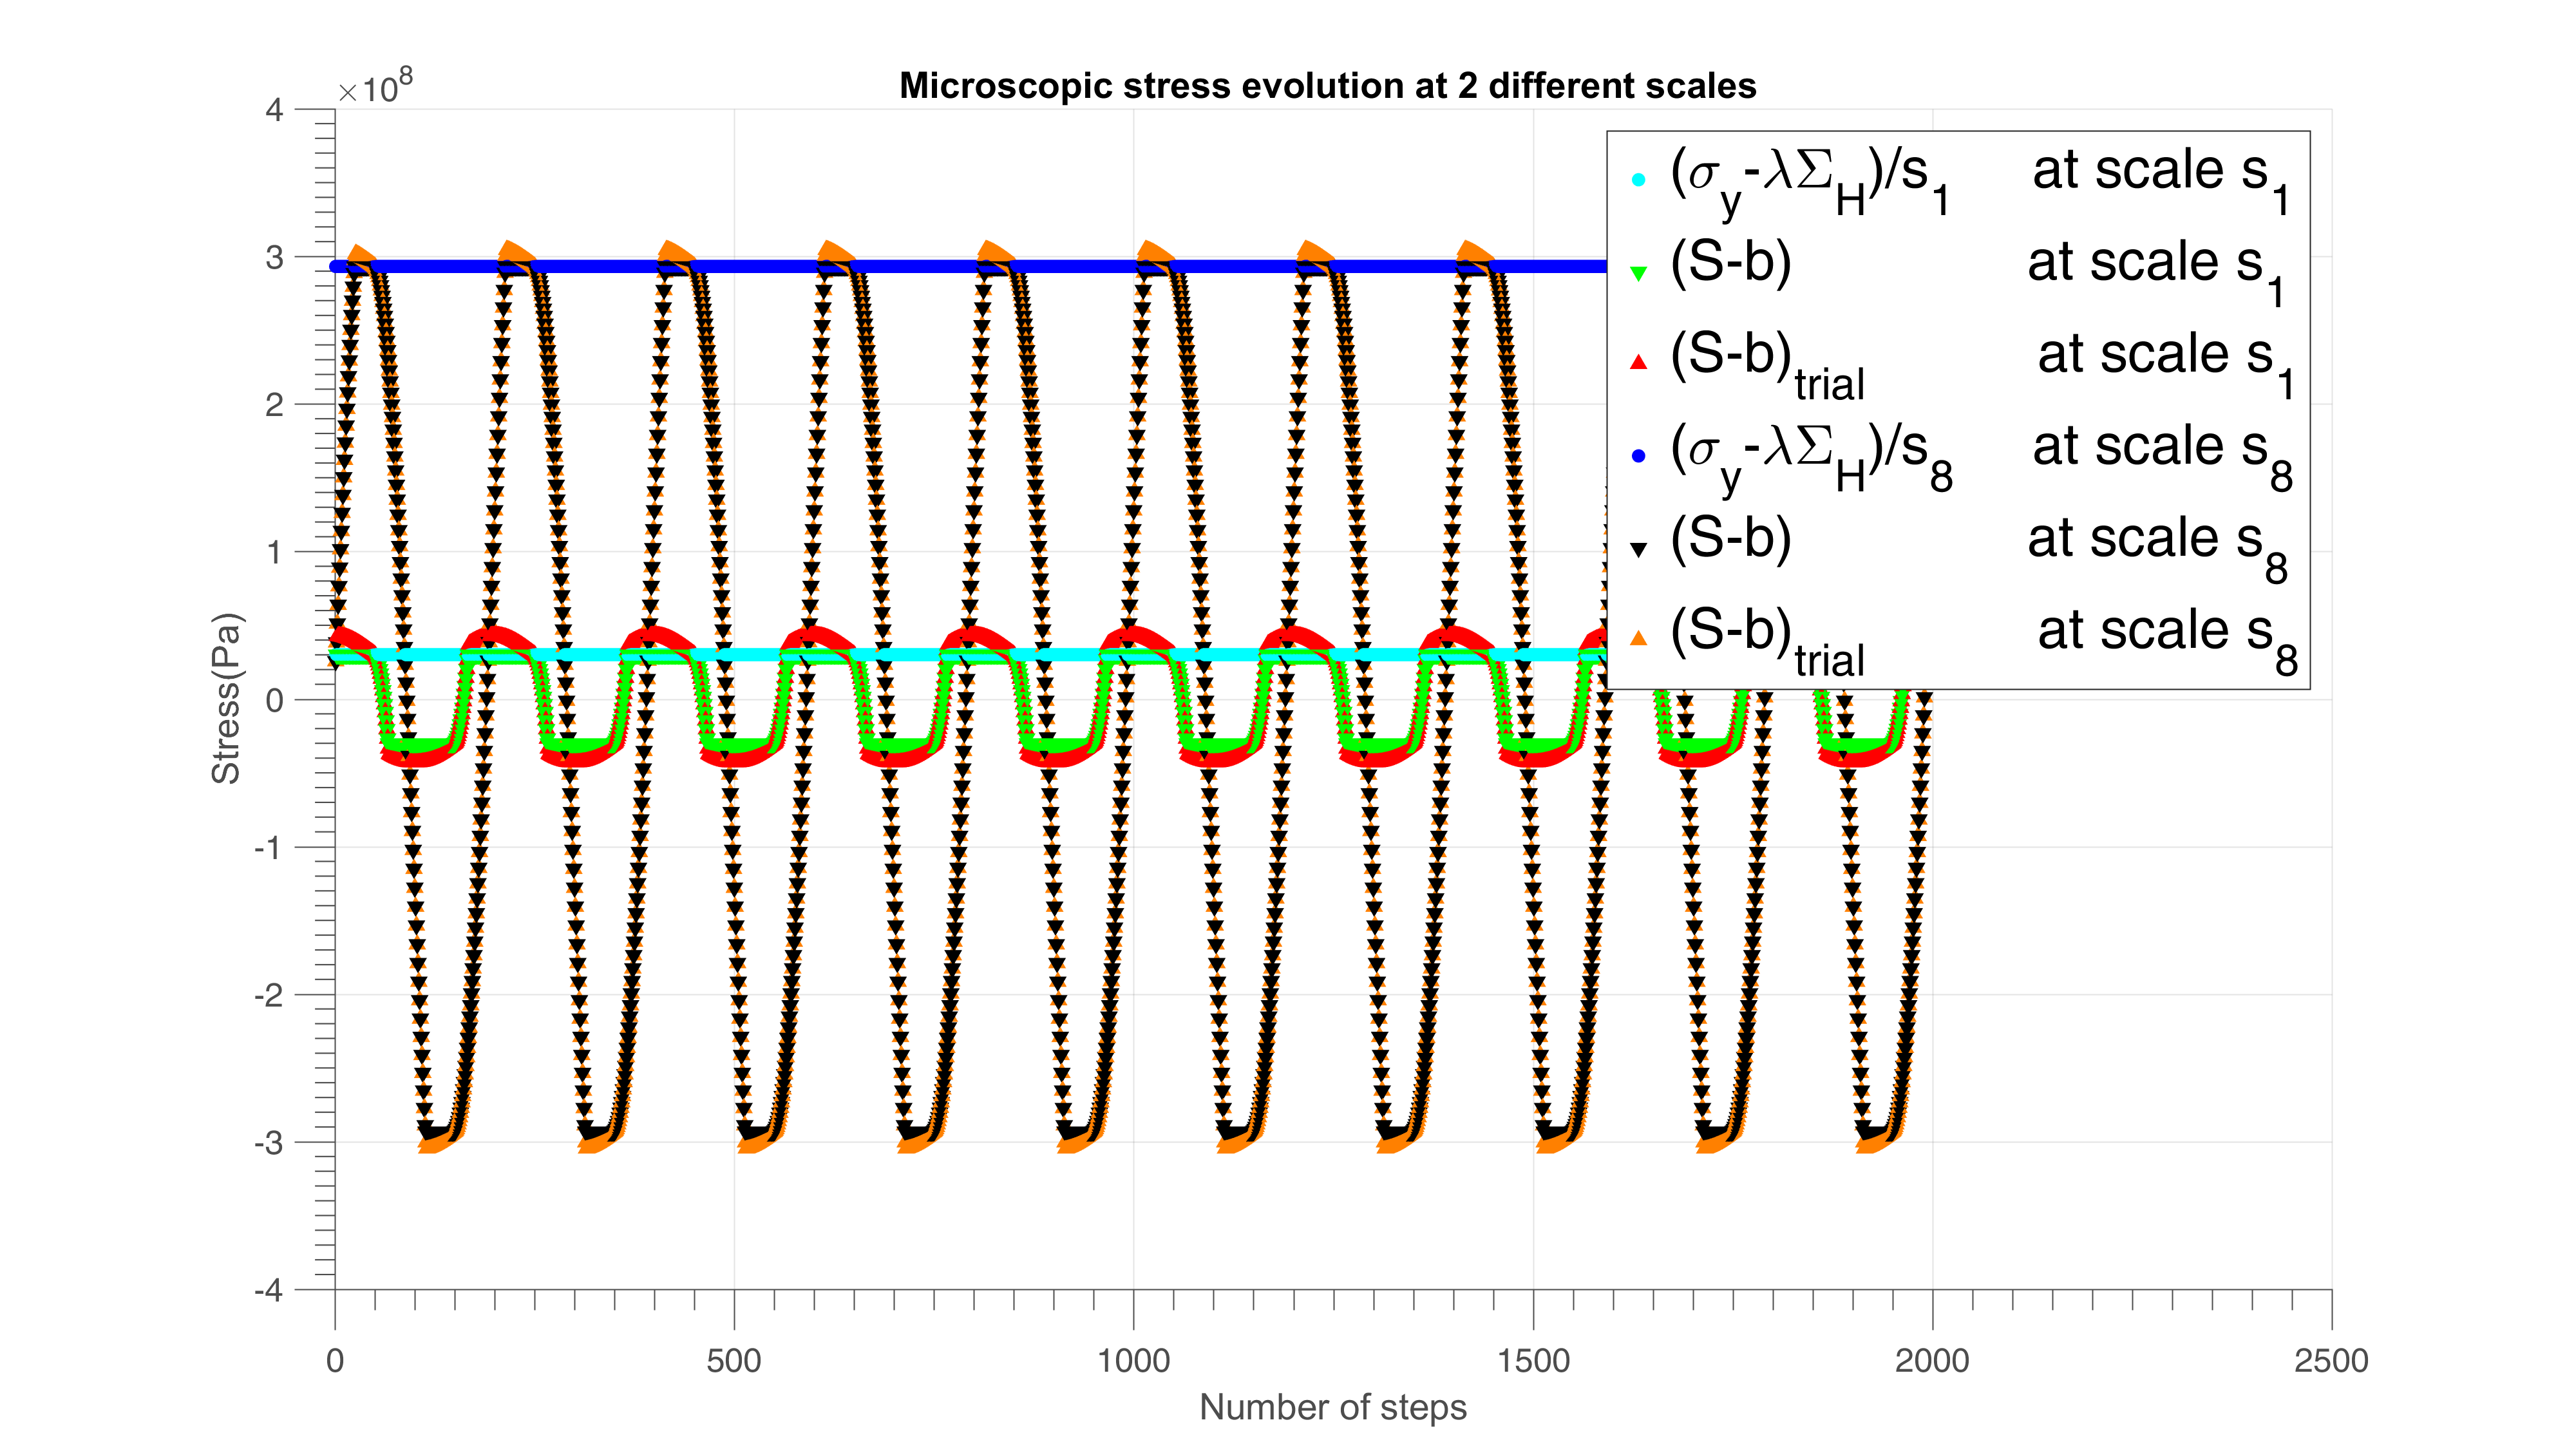
\includegraphics[width=\textwidth]{figures//trialsin.png} 
	\caption{Microscopic $\left( \uline{\uline{S}}-\uline{\uline{b}}\right)_{trial}$ and $\left( \uline{\uline{S}}-\uline{\uline{b}}\right)$ evolution with time under different weakening scales in sinusoidal load}
	\label{trialsin}
\end{figure}

The nonlinearity is determined by 
$$\alpha=1 - a\left\langle \dfrac{\max\limits_{t}\sqrt{J_{2,a}}(t)+a_c{P_{max}(t)}-b_c}{ \sigma_{u} - 2\max\sqrt{J_{2,a}}}\right\rangle,$$ 
which is predominated by Crossland criterion, for simplicity we take $\alpha$ as a constant. The damage evolves like in \figref{damsin}, where we compare the damage evolution as predicted by the cycle accumulation Eq.\eqref{eq:w} and by the numerical strategy of section 4.

\begin{figure}[!h]
	\centering
	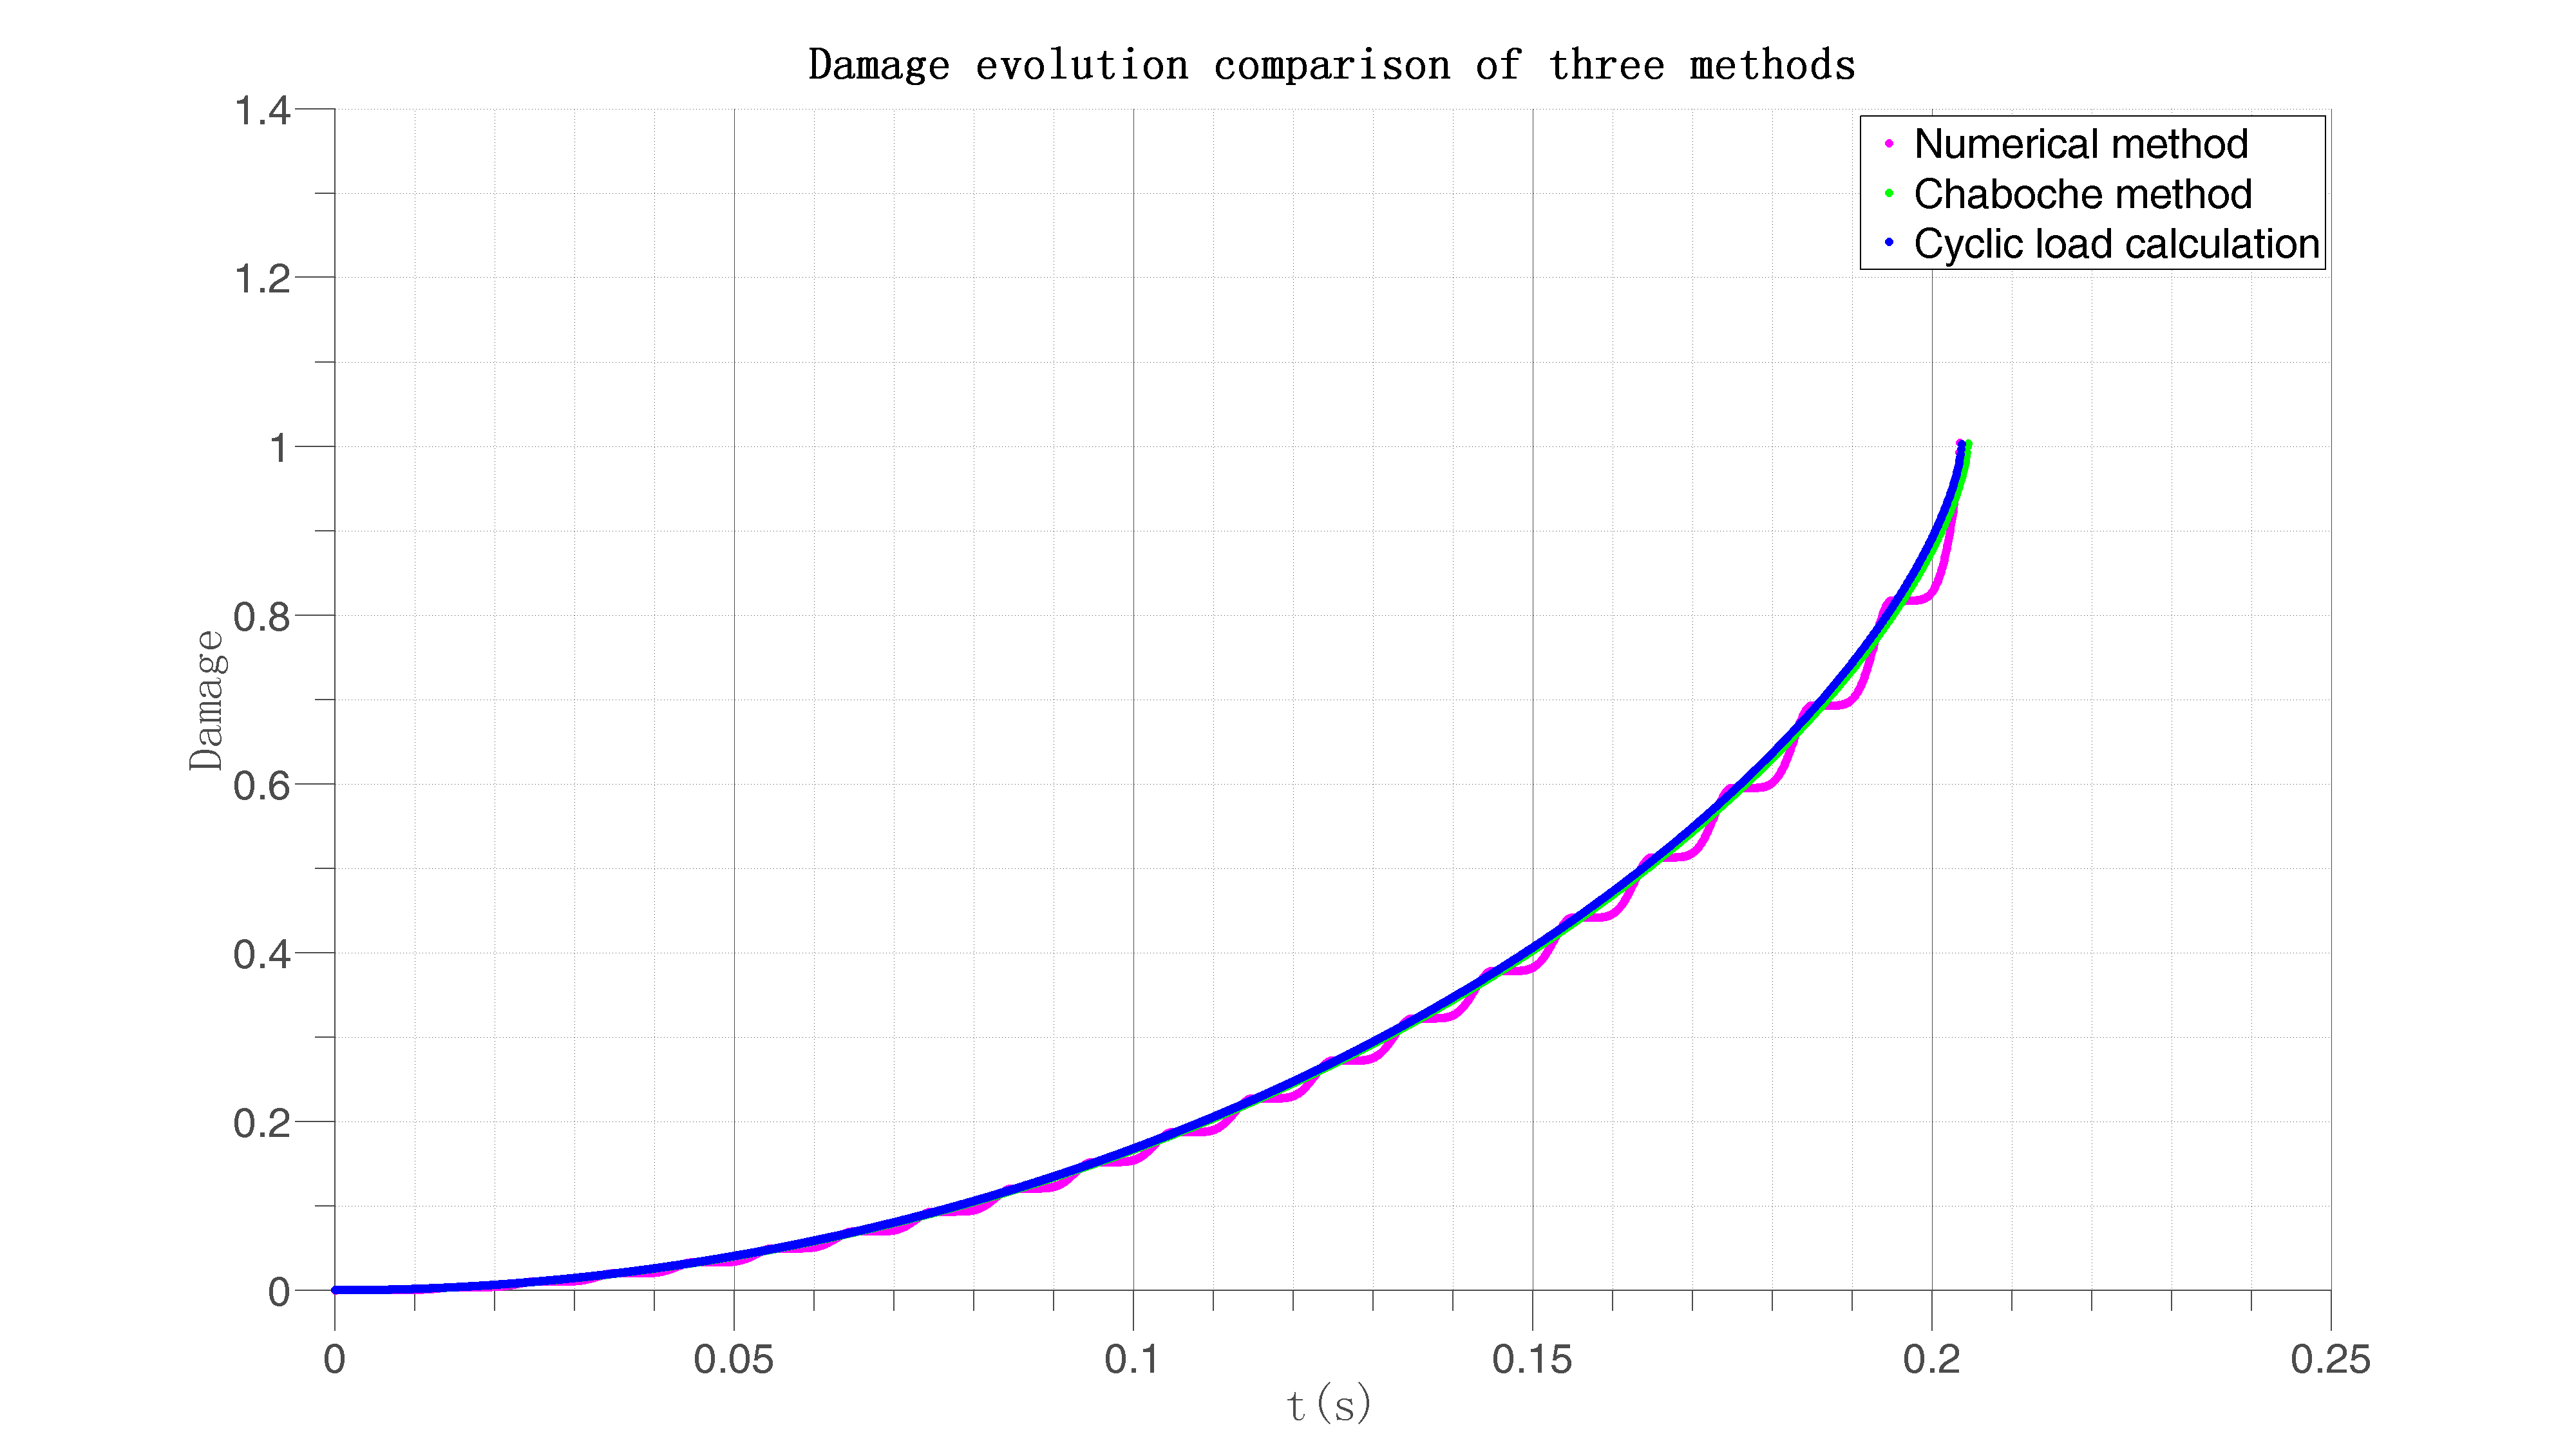
\includegraphics[width=\textwidth]{figures//damagesin.png} 
	\caption{Damage evolution with time under sinusoidal load with two different methods}
	\label{damsin}
\end{figure}

Now we compare the result to the one demonstrated in \figref{backstress}. The first cycle has 3 phases which have the energy loss identical to phase 1. The following cycles each have 4 times energy loss as phase 1. We can see from \figref{NCdiff100} and \figref{NCdiff300} the difference between cyclic load calculation and numerical method as function of time(time step=1/5000s and 1/15000s separately). Because the step by step damage accumulation grows in a power law, so the amplitude of difference grows with time. However, the difference between the two methods swing around 0 and from \figref{damsin} we can see the difference is not symmetrical, we could consider the numerical method converges in cyclic load calculation method.

\begin{figure}[!h]
	\centering
	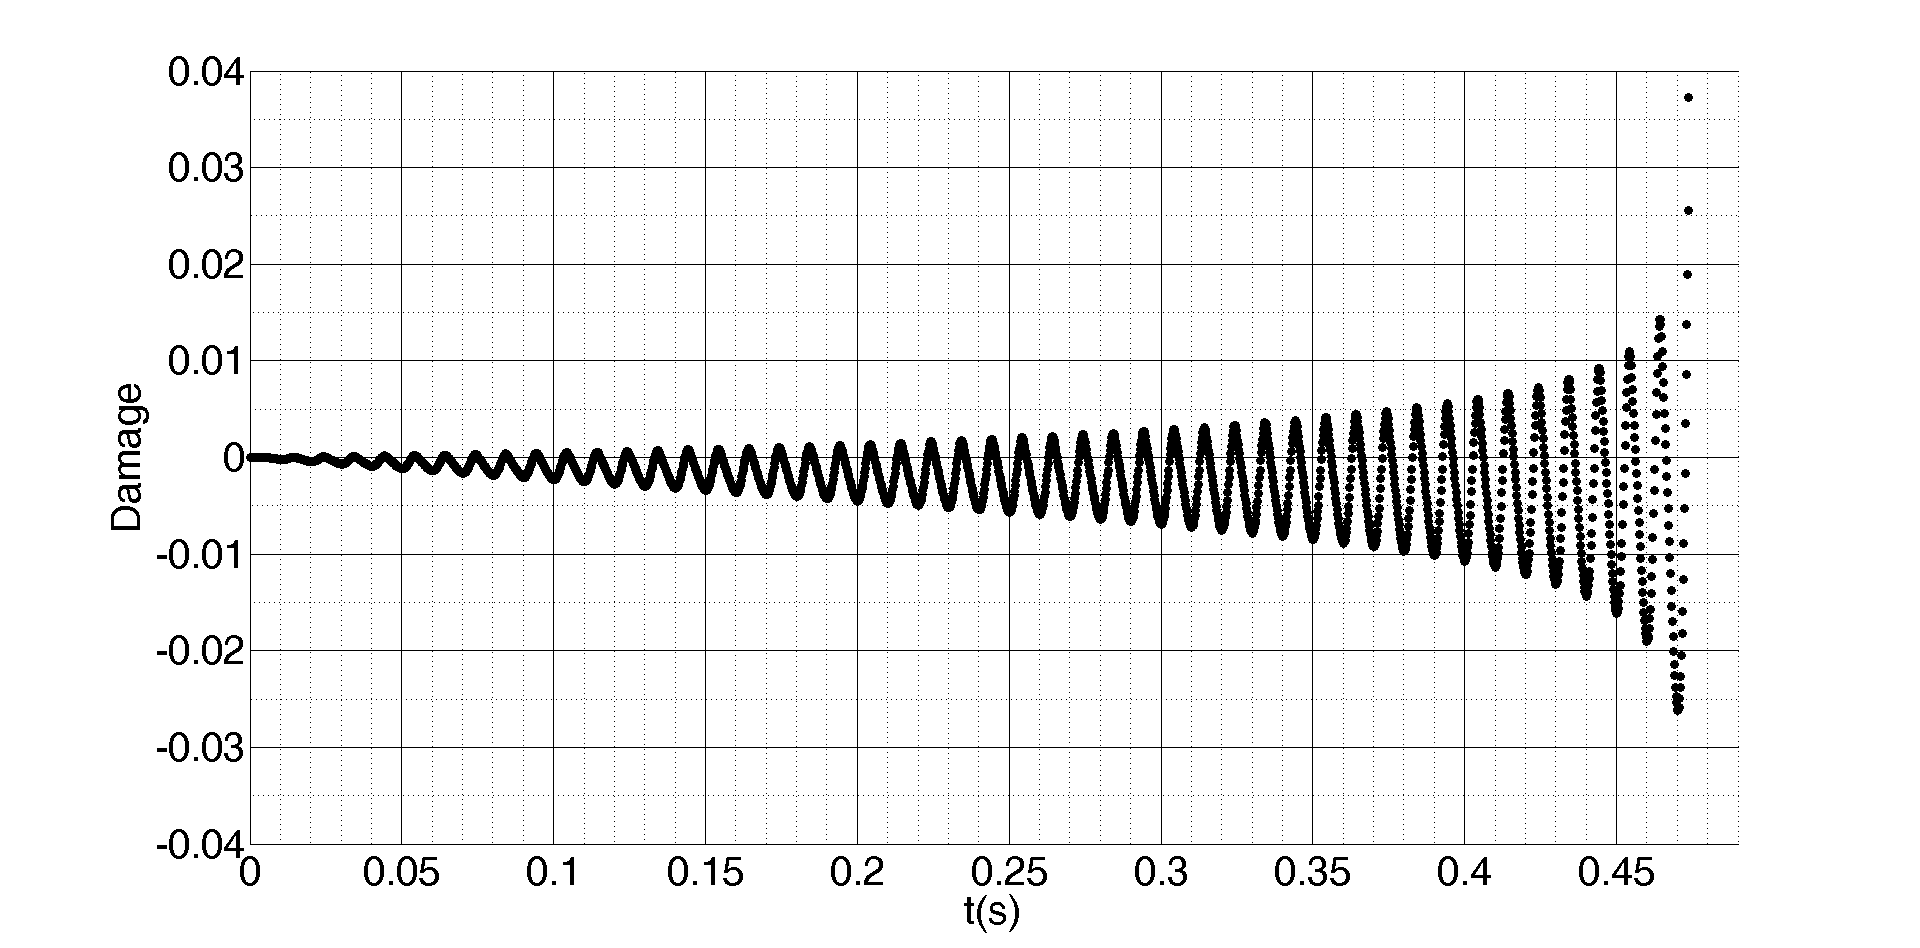
\includegraphics[width=\textwidth]{figures//NCdiff100.png} 
	\caption{Difference between cyclic load calculation and numerical method as function of time(time step=1/5000s)}
	\label{NCdiff100}
\end{figure}
\begin{figure}[!h]
	\centering
	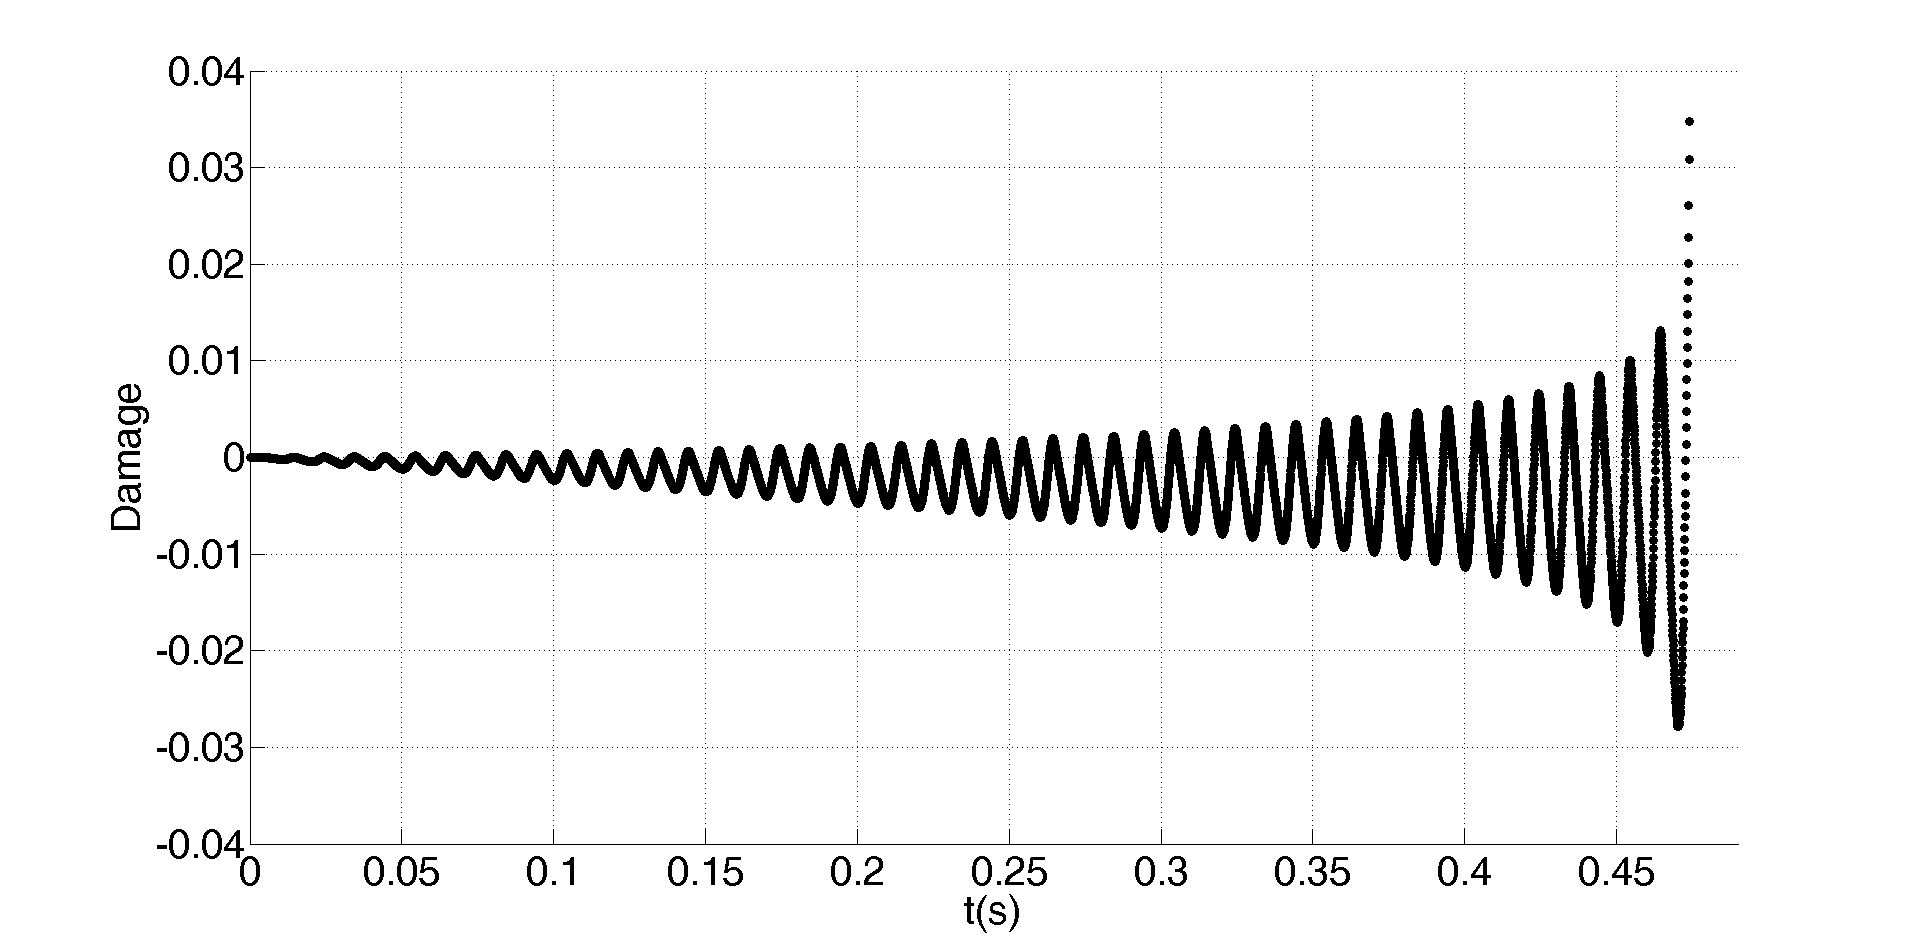
\includegraphics[width=\textwidth]{figures//NCdiff300.png} 
	\caption{Difference between cyclic load calculation and numerical method as function of time(time step=1/15000s)}
	\label{NCdiff300}
\end{figure}
The cyclic load calculation is only valid for very simple such as proportional loading in fatigue, nevertheless it can still be used as a comparison group to verify the numerical results. The outcome seems satisfactory. Hence, to be more general for any loading history, we adopt the numerical method.


\subsubsection{One dimensional application to PSA data}
In this test, we reconstruct a unidimensional macroscopic stress history from recorded force data proposed by PSA group. 
\begin{figure}[!h]
	\centering
	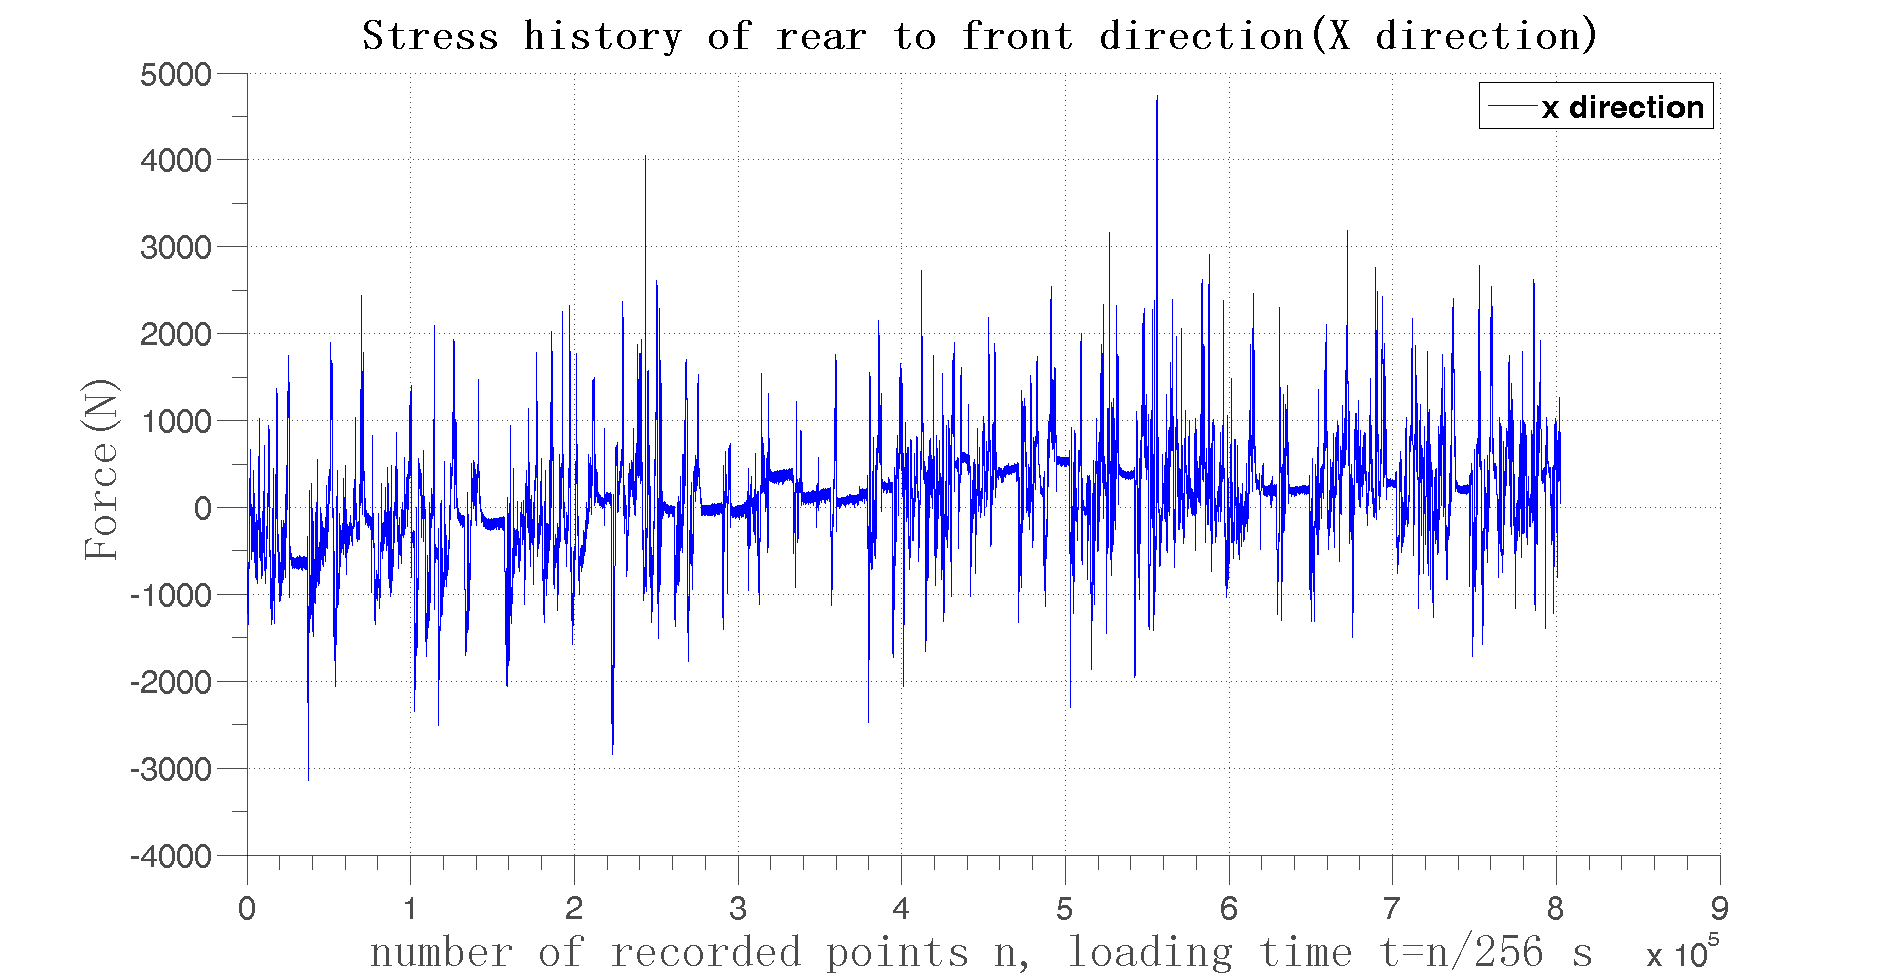
\includegraphics[width=\textwidth]{figures//x.png} 
	\caption{Loading history of X direction, force vs the record index n, with 256 sample recorded per second}
	\label{x}
\end{figure}

The sample recording rate is 256 per second. In order to accumulate damage using very small steps, we have created 10 additional points between every 2 recorded points by linear interpolation. So the sample rate is $256*10$ per second. 

The force on wheel is firstly considered as under uniaxial loading $F_x$. Here we temporally set $\Sigma_x=F_x/A$ where $A=\dfrac{1}{1e6} m^2$ is the area of force, and $W_F=3e6 J$. The other data are as Table.\ref{Sin}. The plot of $\left( \uline{\uline{S}}-\uline{\uline{b}}\right)_{trial}$ and $\left( \uline{\uline{S}}-\uline{\uline{b}}\right)$ under 2 different scales($s_1=21.21657929229650$ and $s_8=2.176132808422946$)are shown in \figref{trialreal}. The damage evolves like \figref{damage1d}.

\begin{figure}[!h]
	\centering
	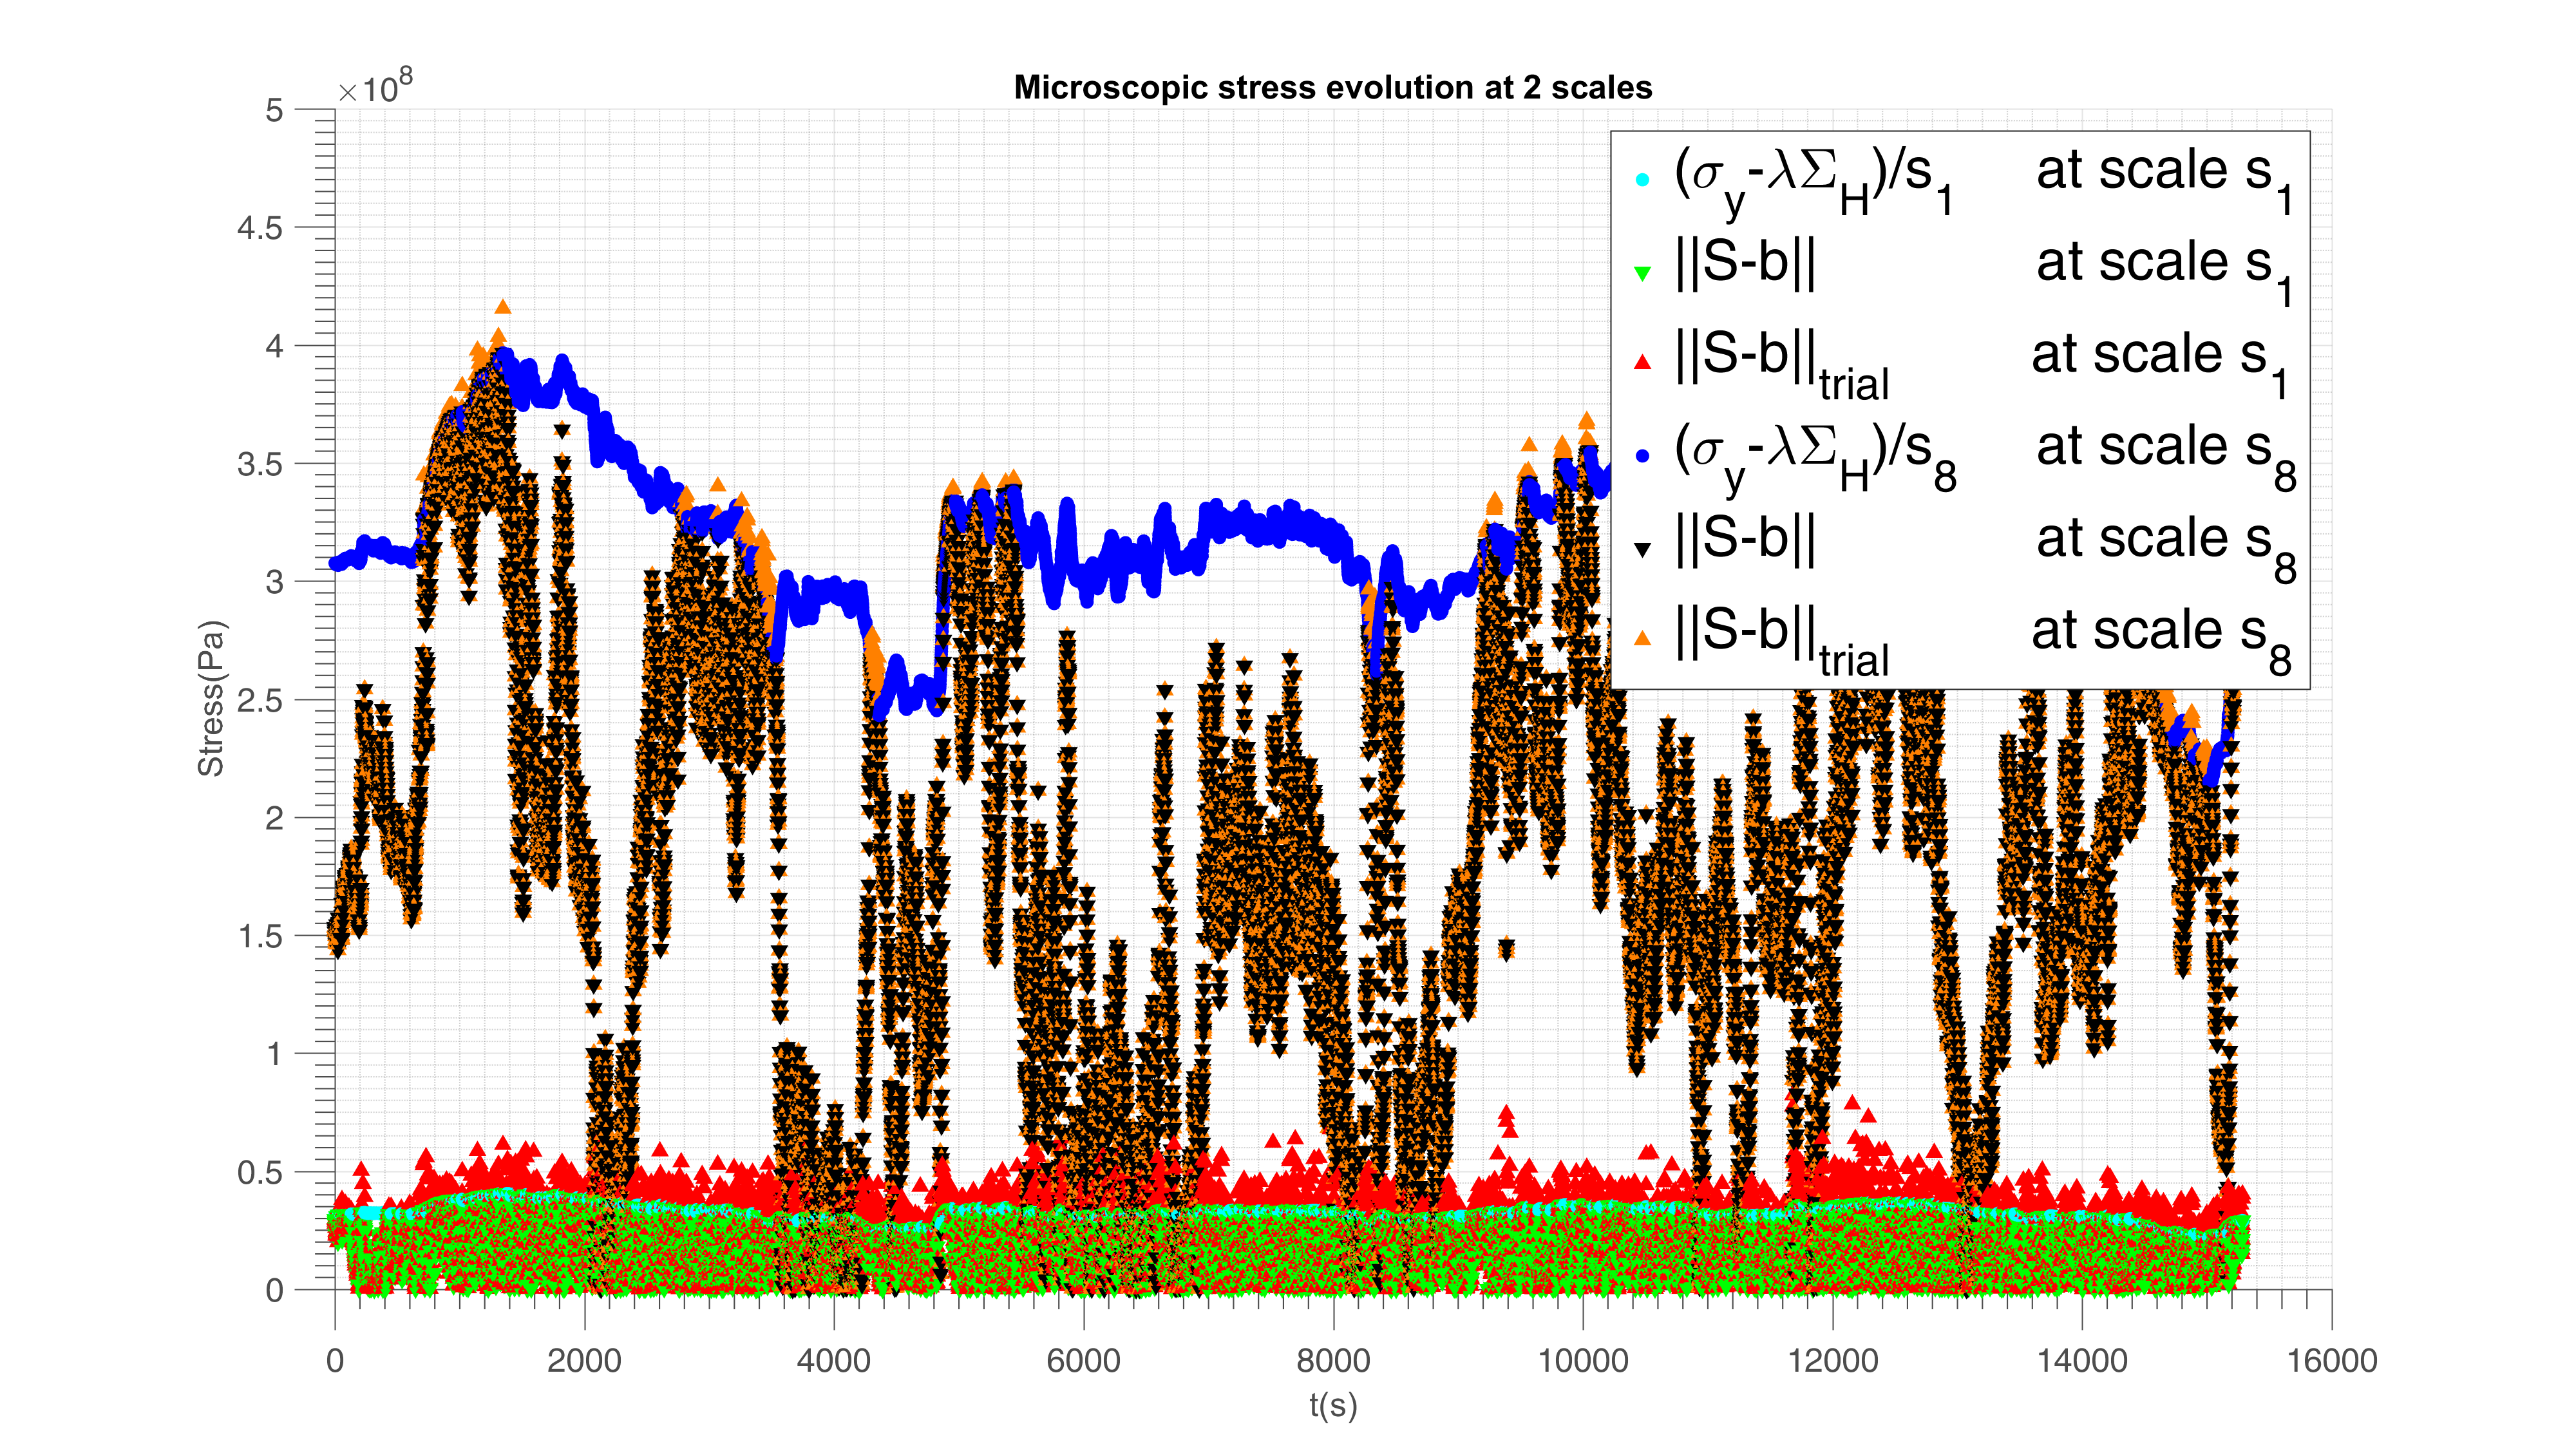
\includegraphics[width=\textwidth]{figures//trialreal1d1.png} 
	\caption{$\left( \uline{\uline{S}}-\uline{\uline{b}}\right)_{trial}$ and $\left( \uline{\uline{S}}-\uline{\uline{b}}\right)$ evolution with time under different weakening scales in PSA load history}
	\label{trialreal}
\end{figure}
\begin{figure}[!h]
	\centering
	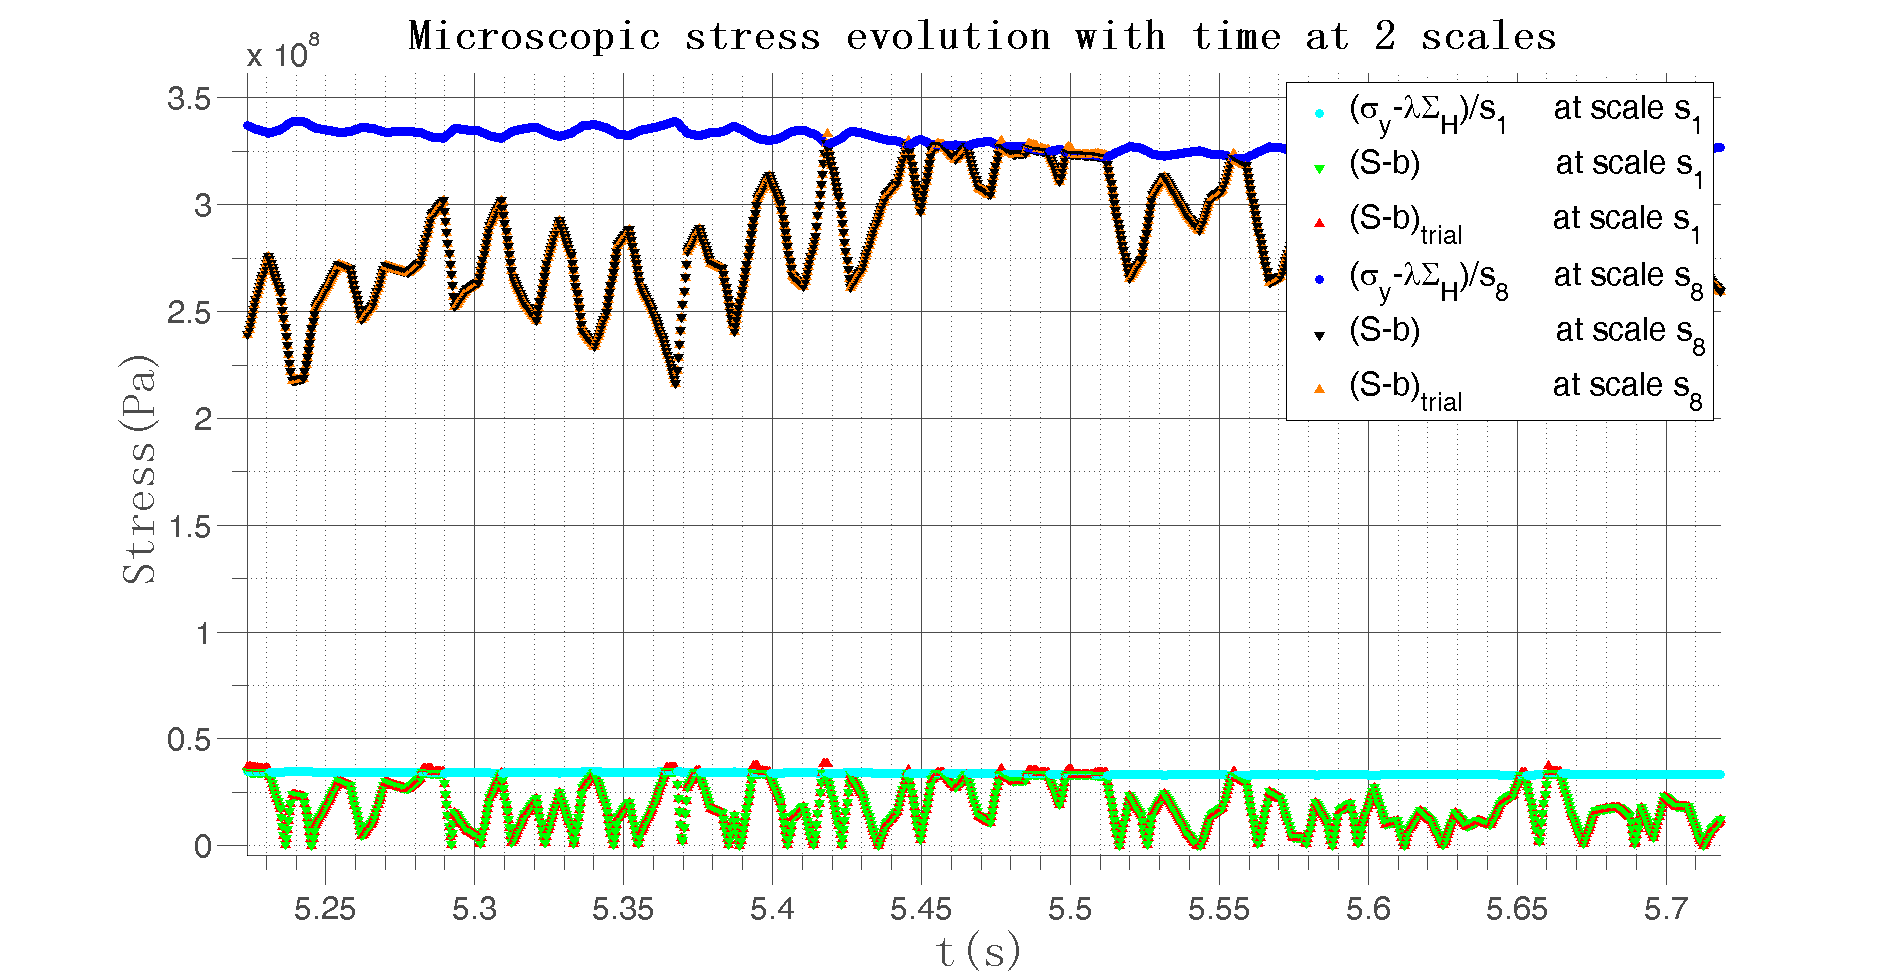
\includegraphics[width=\textwidth]{figures//trialreal1d2.png} 
	\caption{Circled area magnification in \figref{trialreal} where there is more $\left( \uline{\uline{S}}-\uline{\uline{b}}\right)_{trial}>\sigma_y$(plasticity)  at $s_1$ than at $s_8$}
	\label{trialreal1d2}
\end{figure}
\begin{figure}[!h]
	\centering
	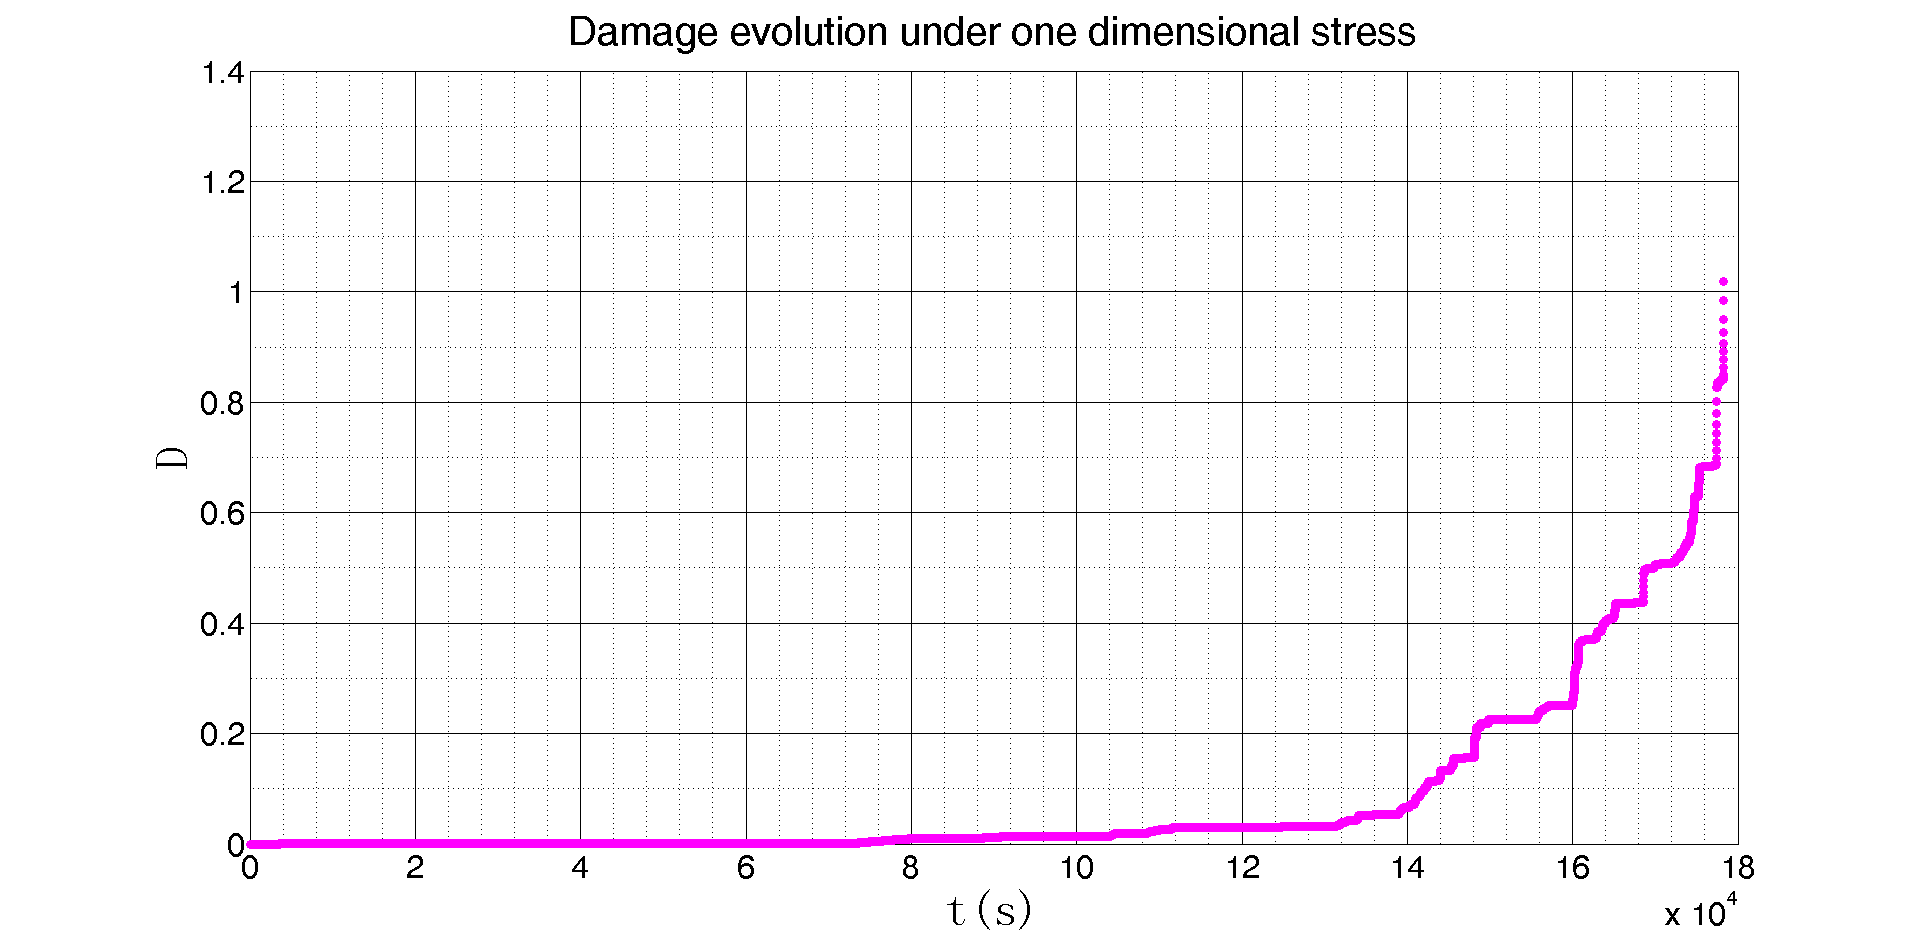
\includegraphics[width=\textwidth]{figures//damage1d.png} 
	\caption{Damage evolution with time at one dimension PSA load history}
	\label{damage1d}
\end{figure}

\newpage
\subsubsection{Multi-dimensional application to PSA data}
We now consider a situation where we have force recorded measured in 3 different directions as shown in \figref{xyz}.
\begin{figure}[!h]
	\centering
	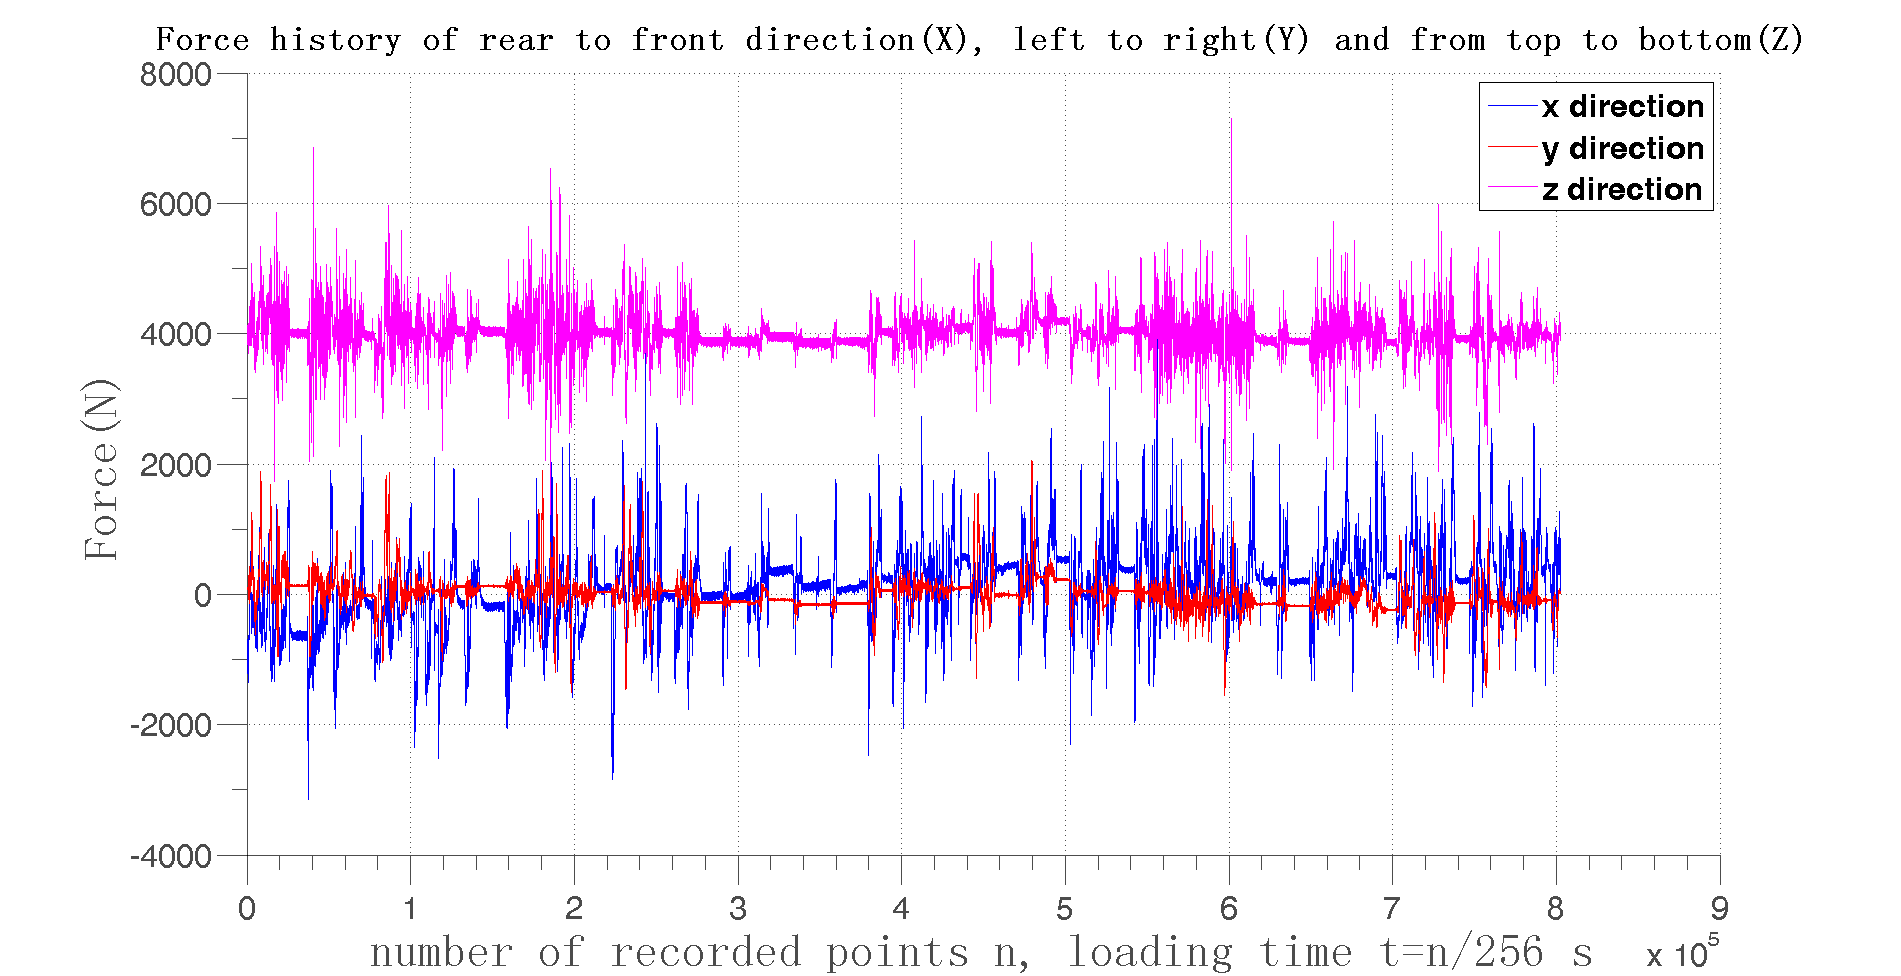
\includegraphics[width=\textwidth]{figures//xyz.png} 
	\caption{Loading history of 3 different directions}
	\label{xyz}
\end{figure}
\begin{figure}[!h]
	\centering
	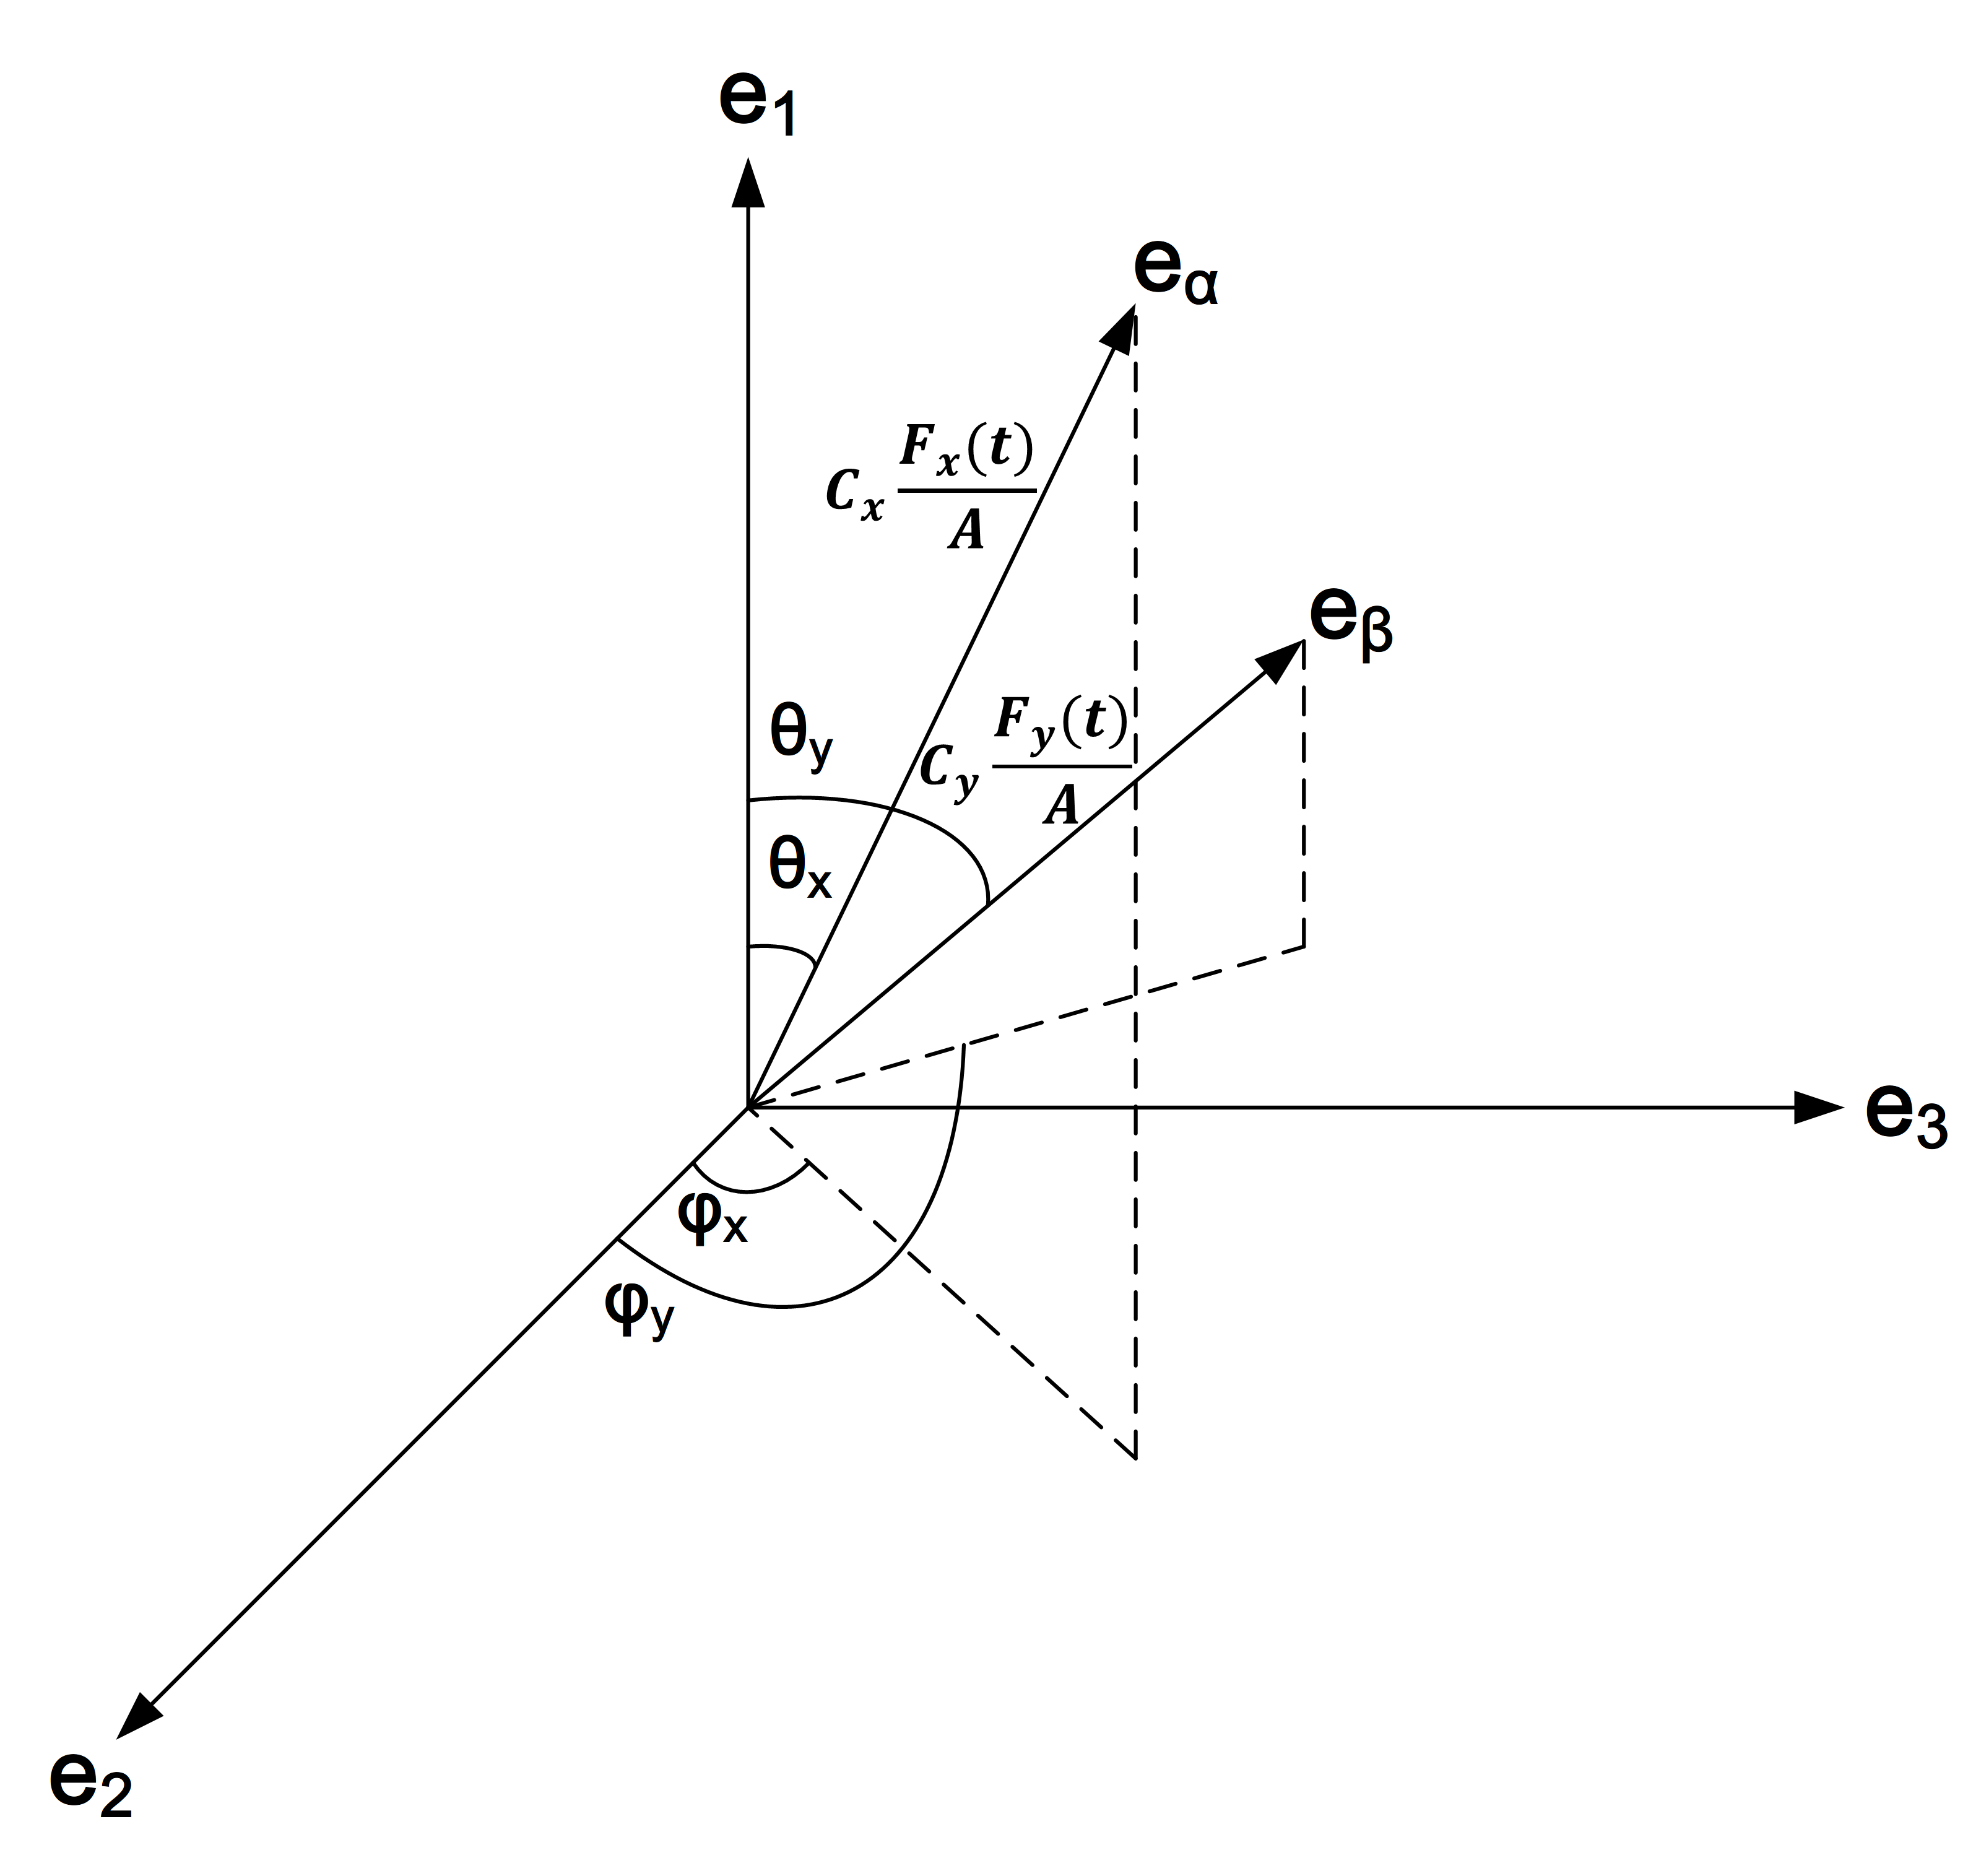
\includegraphics[width=0.7\textwidth]{figures//xab.png} 
	\caption{Loading in 3 different directions}
	\label{xab}
\end{figure}
In real case, the vertical force $F_z$ is much larger than the axial and horizontal forces $F_x$ and $F_y$, as shown in \figref{xyz}. However, in order to investigate large domains of interest, we first scale the axial and horizontal forces to reach comparable impact and transform them in principal stresses $c_x\dfrac{F_x}{A}$ applied along the stress principle vector $\uline{e}_\alpha$(respectively $\uline{e}_\beta$) that we choose randomly(\figref{xab}). We therefore consider the following macroscopic stress tensor:
\begin{equation}
	\uline{\uline{\Sigma}}=\dfrac{F_z(t)}{A}\uline{e}_1\otimes \uline{e}_1+c_x\dfrac{F_x(t)}{A}\uline{e}_{\alpha}\otimes \uline{e}_{\alpha}+c_y\dfrac{F_y(t)}{A}\uline{e}_{\beta}\otimes \uline{e}_{\beta}
	\label{tensor1}
\end{equation}
where $\uline{e}_{\alpha}$  and $\uline{e}_{\beta}$ are principal vectors whose spherical coordinate are $\theta_x$, $\varphi_x$,  $\theta_y$ and $\varphi_y$ respectively:
$$\uline{e}_{\alpha}=cos\theta_x\uline{e}_1+sin\theta_xcos\varphi_x\uline{e}_2+sin\theta_xsin\varphi_x\uline{e}_3,$$
$$\uline{e}_{\beta}=cos\theta_y\uline{e}_1+sin\theta_ycos\varphi_y\uline{e}_2+sin\theta_ysin\varphi_y\uline{e}_3.$$
Here $F_x(t)$, $F_y(t)$, $F_z(t)$ are from test data, and $\theta_x$, $\varphi_x$, $\theta_y$, $\varphi_y$ are structural parameters to be chosen randomly.The physical data are the same with parameters in Table.\ref{Sin}. The structural data we choose is shown in Table.\ref{structural}.

\begin{table}[!h]
	\centering
	\begin{tabular}{rrrrrrrr}
		\hline
		\textbf{Parameter} & A($m^2$) & $c_x$ & $c_y$ & $\theta_x$ & $\varphi_x$ & $\theta_y$ & $\varphi_y$ \\
		\textbf{Value}      & 1/6e4                  & 10    & 60    & 0.5        & 0.3         & 0.6        & 0.4         \\ \hline
	\end{tabular}
	\caption{The structural data in 3D analysis}
	\label{structural}
\end{table}

The underlying assumption is that a unit load on wheel in direction $\uline{e}_x$ creates a stress tensor at point $M$ given by:
$$c_x\dfrac{F_x(t)}{A}\uline{e}_{\alpha}\otimes \uline{e}_{\alpha},$$
where $\uline{e}_{\alpha}\otimes \uline{e}_{\alpha}$ defines the local structural response of the vehicle.

Replacing $\uline{e}_{\alpha}$ and $\uline{e}_{\beta}$ in Eq.\eqref{tensor1} we get the stress tensor in Eq.\eqref{tensor2}. 
 \begin{equation}
 	\begin{split}
 		\uline{\uline{\Sigma}}=&\dfrac{F_z}{A}\uline{e}_1\otimes \uline{e}_1+c_x\dfrac{F_x}{A}\uline{e}_{\alpha}\otimes \uline{e}_{\alpha}+c_y\dfrac{F_y}{A}\uline{e}_{\beta}\otimes \uline{e}_{\beta}
 		\\=&\dfrac{F_z}{A}\uline{e}_1\otimes \uline{e}_1+c_x\dfrac{F_x}{A}\left(cos\theta_x\uline{e}_1+sin\theta_xcos\varphi_x\uline{e}_2+sin\theta_xsin\varphi_x\uline{e}_3 \right) \otimes\left(cos\theta_x\uline{e}_1+sin\theta_xcos\varphi_x\uline{e}_2+sin\theta_xsin\varphi_x\uline{e}_3 \right)
 		\\&+c_y\dfrac{F_y}{A}\left( cos\theta_y\uline{e}_1+sin\theta_ycos\varphi_y\uline{e}_2+sin\theta_ysin\varphi_y\uline{e}_3\right) \otimes\left( cos\theta_y\uline{e}_1+sin\theta_ycos\varphi_y\uline{e}_2+sin\theta_ysin\varphi_y\uline{e}_3\right)
 		\\=&\left(\dfrac{F_z}{A} +c_x\dfrac{F_x}{A}cos^2\theta_x+c_y\dfrac{F_zy}{A}cos^2\theta_y\right) \uline{e}_1\otimes \uline{e}_1
 		\\&+\left(c_x\dfrac{F_x}{A}cos\theta_xsin\theta_x cos\varphi_x+c_y\dfrac{F_y}{A}cos\theta_ysin\theta_y cos\varphi_y\right) \left( \uline{e}_1\otimes \uline{e}_2+\uline{e}_2\otimes \uline{e}_1\right) 
 		\\&+\left(c_x\dfrac{F_x}{A}cos\theta_xsin\theta_x sin\varphi_x+c_y\dfrac{F_y}{A}cos\theta_ysin\theta_y sin\varphi_y\right) \left( \uline{e}_1\otimes \uline{e}_3+\uline{e}_3\otimes \uline{e}_1\right) 
 		\\&+\left(c_x\dfrac{F_x}{A}sin^2\theta_xcos^2\varphi_x+c_y\dfrac{F_y}{A}sin^2\theta_y cos^2\varphi_y\right) \uline{e}_2\otimes \uline{e}_2
 		\\&+\left(c_x\dfrac{F_x}{A}sin^2\theta_x cos\varphi_xsin\varphi_x+c_y\dfrac{F_y}{A}sin^2\theta_y cos\varphi_ysin\varphi_y\right) \left( \uline{e}_2\otimes \uline{e}_3+\uline{e}_3\otimes \uline{e}_2\right) 
 		\\&+\left(c_x\dfrac{F_x}{A}sin^2\theta_xsin^2\varphi_x+c_y\dfrac{F_y}{A}sin^2\theta_y sin^2\varphi_y\right) \uline{e}_3\otimes \uline{e}_3
 	\end{split}
 	\label{tensor2}
 \end{equation}
 
The plot of $\left( \uline{\uline{S}}-\uline{\uline{b}}\right)_{trial}$ and $\left( \uline{\uline{S}}-\uline{\uline{b}}\right)$ under 2 different scales are shown in \figref{trialreal3d}.
\begin{figure}[!h]
	\centering
	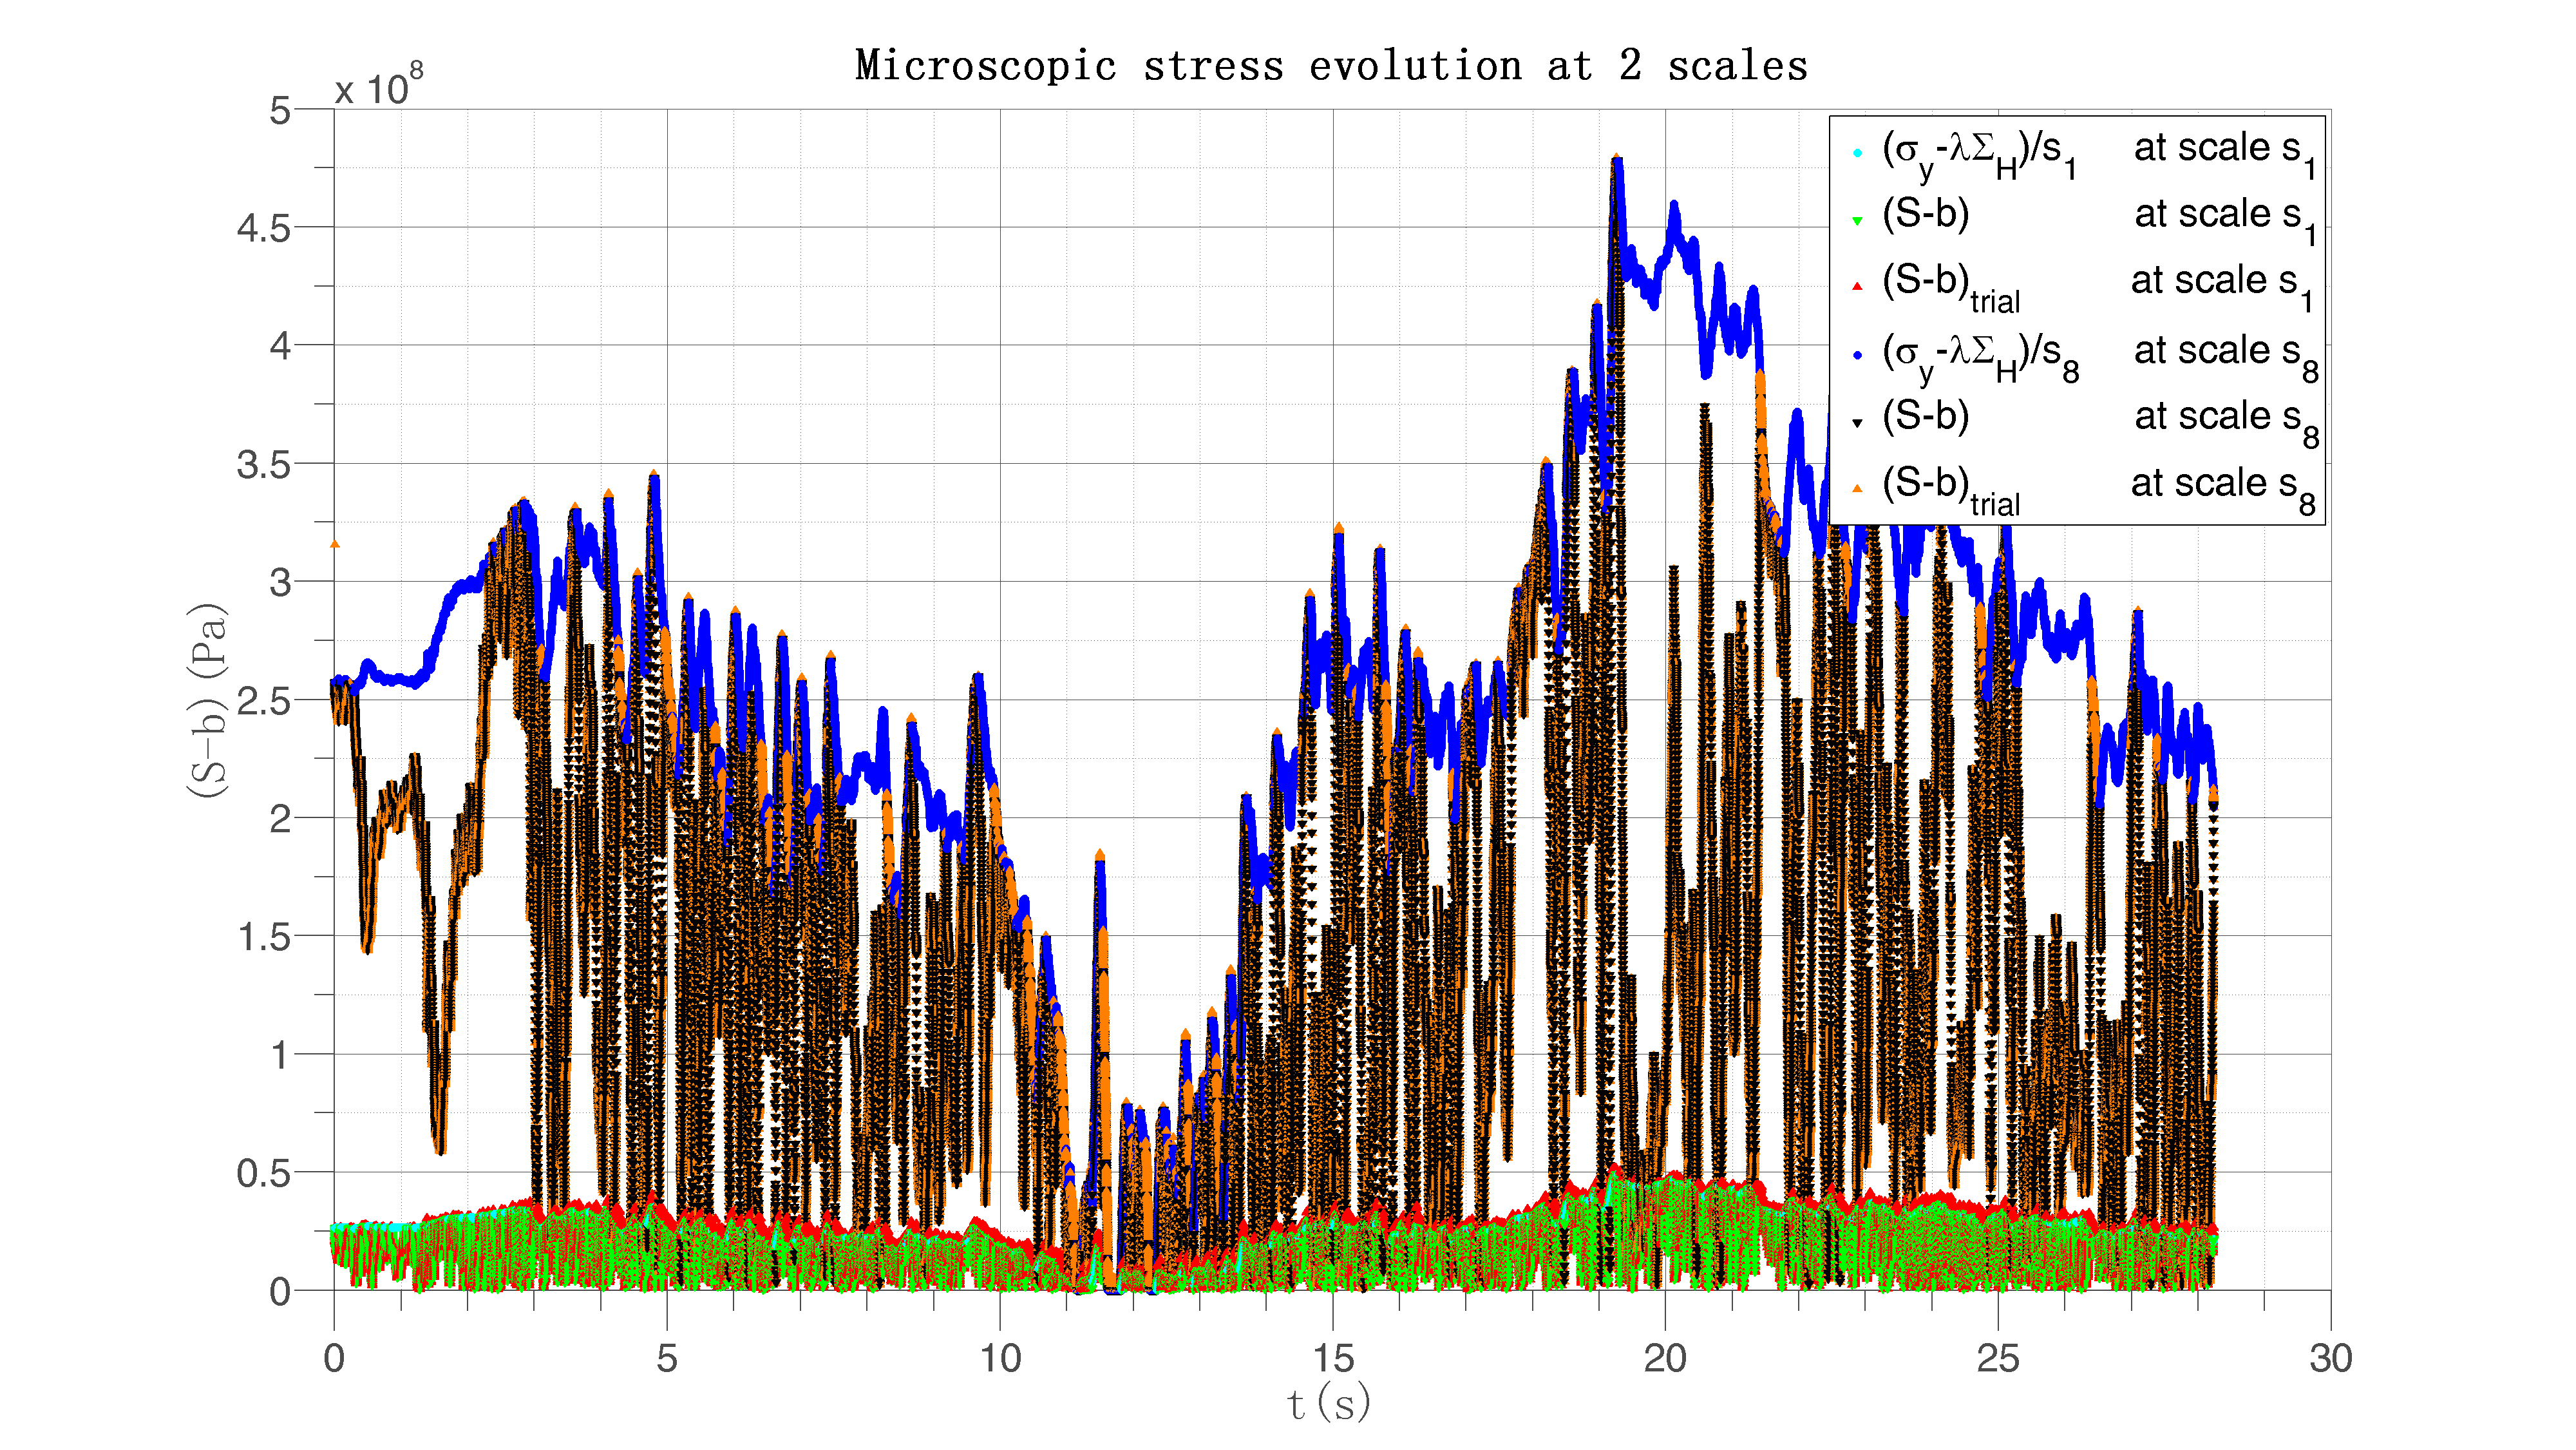
\includegraphics[width=\textwidth]{figures//trialreal3d.png} 
	\caption{$\left( \uline{\uline{S}}-\uline{\uline{b}}\right)_{trial}$ and $\left( \uline{\uline{S}}-\uline{\uline{b}}\right)$ evolution with time under different weakening scales in PSA load history}
	\label{trialreal3d}
\end{figure} 

In the load history, when $\left( \uline{\uline{S}}-\uline{\uline{b}}\right)_{trial}>\sigma_y$, the damage accumulates. However, under scale $s_{10}$, there are much less damage accumulation than under scale $s_1$. In this way we do not neglect the small influences in load history and the big fluctuation in stress is magnified which reflects the real situation.

%\iffalse
The damage evolves like in \figref{dam3d}. 


\begin{figure}[!h]
	\centering
	\includegraphics[width=\textwidth]{figures//damage3d.png} 
	\caption{Damage evolution under multidimensional stress}
	\label{dam3d}
\end{figure}
%\fi

We can improve the result by inserting more arithmetic sequence points between every 2 recorded points. As is shown in Table.\ref{steppoints} :

\begin{table}[!h]
	\centering
	\caption{Arithmetic sequence points density effect}
	\label{steppoints}
	\begin{tabular}{cc}
		\hline
		\textbf{Arithmetic sequence points between every two points} & \textbf{Total time to failure(s)} \\ \hline
		10                                                           & 78.63711                          \\ 
		20                                                           & 72.24630                          \\ 
		30                                                           & 70.25793                          \\ 
		50                                                           & 68.69148                          \\ 
		100                                                          & 67.49223                          \\ \hline
	\end{tabular}
\end{table}

\subsection{Discussion}

The strategy can be made more complex by introducing a local space averaging process in the calculation of the local damage, and by taking more general plastic flows. The energy based fatigue approach takes into account impurities and hardness in the material which affect the fatigue life. The load sequence effects for complex multiaxial loading history are included in damage accumulation process. The small step-by-step strategy does not ignore small fluctuations in the load history. In addition, it can take into account any type of micro plasticity law and multiaxial load geometry.

Further research of energy based failure criteria should be focused on the following aspects:
\begin{enumerate}
	\item The  accommodation law might be more elaborate than kinematic hardening.
	
	\vspace{6pt}
	\item The differentiation of shear stress and normal stress effect on fatigue life should be clarified.
	
	\vspace{6pt}
	\item The non-linearity parameter $\alpha$ contains the stress $\sigma$, so it can evolve with time. But for complex loading history, should it change at every time step?
	
\end{enumerate}


\section{Multi-dimensional application}

We have a 52 minutes recording of an average customer which have driven 18.3 kilometers. A complete set of forces were recorded at the center of the left front wheel (LFW in English but RAVG in French for Roue AVant Gauche). This wheel is driving and sustains the engine mass (half of it).\\
FX: Force in the axial direction (from rear to front), a positive (resp. negative) force corresponds to an acceleration (resp. deceleration) of the vehicle.\\
FY: Force in the horizontal direction (from driver to shotgun), a positive (resp. negative) force corresponds to an right (resp. left) turn.\\
FZ: Force in the vertical direction (from top to bottom), a more (resp. less) than average force corresponds to a bump (resp. pot hole) in the road, the average is the vehicle mass to the wheel.\\

The summary of the signals are :
\begin{table}[]
	\centering
	\begin{tabular}{llll}
		\hline
		\multicolumn{1}{c}{\textbf{Loading direction}} & \multicolumn{1}{c}{\textbf{max(N)}} & \multicolumn{1}{c}{\textbf{mean(N)}} & \multicolumn{1}{c}{\textbf{min(N)}} \\ \hline
		FX\_RAVG                                       & 4739                                & 113                                  & -3145                               \\
		FY\_RAVG                                       & 2050                                & 0                                    & -1558                               \\
		FZ\_RAVG                                       & 7301       & 4012                                 & 1219                                \\
		FZ\_RARG                                       & 5858                                & 3272                                 & 647                                 \\ \hline
	\end{tabular}
	\caption{Summary of the signals in the center of LFW}
	\label{data}
\end{table}


\begin{figure}[h!]
	\centering
	\includegraphics[width=\textwidth]{figures//fx.png} 
	\caption{Fx in the Left Front Weel with points recorded}
	\label{fx}
\end{figure}

From a comparison point of view, the rainflow counting in the Range/Mean diagram of these signals gives:

\begin{table}[]
	\centering
	\caption{My caption}
	\label{rain}
	\begin{tabular}{lllll}
		\hline
		\multicolumn{1}{c}{\textbf{Signal}} & \multicolumn{1}{c}{\textbf{nb of cycles}} & \multicolumn{1}{c}{\textbf{Max of Range}} & \multicolumn{1}{c}{\textbf{Min of Mean}} & \multicolumn{1}{c}{\textbf{Max of Mean}} \\ \hline
		\textbf{FX\_RAVG}                   & 206636                                    & 7884                                      & -3106                                    & 4704                                     \\
		\textbf{FY\_RAVG}                   & 205359                                    & 3608                                      & -1489                                    & 2032                                     \\
		\textbf{FZ\_RAVG}                   &237703             & 6082                                      & 2225                                     & 6224                                     \\
		\textbf{FZ\_RARG}                   & 340967                                    & 5211                                      & 1482                                     & 5122                                     \\ \hline
	\end{tabular}
	\caption{Rainflow counting results of the force data}
	\label{rf}
\end{table}


So all the signals present a significant amounts of fatigue cycles (above 2e5) but the rear wheel is richer (by 50\%), hence it is presented here.

The starting point is the data of a loading history on different macroscopic directions $(\uline{F}_i)_i=1,N$ . Typically, in the data sent recently by PSA, the elementary loads are the three components of the force applied at the rear center wheel  $(q_i(t))_i=1,N$. The objective is to construct from this data a multi-scale stochastic mesoscopic plastic damage accumulation at the different materials points $M$ inside the structure, and identify the time to failure as the time when the cumulated energy dissipated by this mesoscopic plastic accumulation reaches a given material threshold.

The material under high cycle fatigue does not undergo local strain concentration. But physically the internal residual stress causes slip of grains in the weaker parts in the material. The grain slip system is determined by the orientation of the stress and the size of grain. To predict failure we have to consider both shear and hydrostatic stress of the loading.

The whole process of loading history has no macroscopic plastic deformation. But instead of thinking mesoscopic stress concentration, we assume there are local weak points where the stress yield limit is smaller than the macroscopic one. To put this thought into formula we assume the mesoscopic strain is the same as macroscopic strain:
$$\hat{\varepsilon}=E$$
And the mesoscopic shear stress is the difference between macroscopic stress and the local residual stress.
$$\hat{\sigma}=\Sigma-\hat{\sigma_R}$$

To get the residual stress evolution with time we need to find a filter to get rid of the  signals with small variation which have negligible influence on residual stress, see \figref{filtered}. The filtered rainflow signal 'shortened' the actual time that the material endured but this does not influent our damage prediction because we consider the trivial signals has no impact on fatigue life.

\begin{figure}[h!]
	\centering
	\includegraphics[width=\textwidth]{figures//filtered.png} 
	\caption{Comparison between the recorded signal and filtered signal which removes the small variation points where the rainflow cycle amplitude $h\leqslant 100N$}
	\label{filtered}
\end{figure}

From the filtered loading history we use Dang Van or Habbibou's law to get the residual stress evolution history at given slip(orientation) or scale. By making the difference between the actual stress and residual stress we get $\hat{\sigma}$. 

When the accumulated energy reached a certain limit then fatigue occurs. Locally we have the expression of dissipated energy:
$$\Delta W\doteq\int\hat{\sigma}:\hat{\varepsilon}dt$$

To start with simple case we assume our signal is sinusoidal. Now we want the distribution of orientation of the slips in the metal. Statistics method gives us the yield limit distribution.


\vspace{6pt}
\noindent
\textbf{Acknowledgments}
\vspace{6pt}
We are grateful for the financial and technical support of Chaire PSA.


\clearpage
\bibliographystyle{unsrt}
\bibliography{11thesis}
\addcontentsline{toc}{section}{Reference}


\clearpage
\appendix
\appendixpage
\addcontentsline{toc}{section}{Appendices}\markboth{APPENDICES}{}
\lstset{% general command to set parameter(s)
	basicstyle=\small, 
	keywordstyle=\color{red}, 
	identifierstyle=, % nothing happens
	commentstyle=\color{blue}, 
	stringstyle=\ttfamily, % typewriter type for strings
	showstringspaces=false} % no special string spaces
%\begin{subappendices}
%	\section{DETAILED EXPLOITATION}
%	************************************************************************************

 A DETAILED DESCRIPTION OF ANALYTICAL EXPLOITATION ON UNIAXIAL CYCLE
 
\noindent              
************************************************************************************

\noindent
\textbf{Phase 1:} The deviatoric stress amplitude increases from $\sigma_y/s$ to $S_{max}$.

\noindent
The material is in local plastic regime, then $\dot{\varepsilon}^p>0$ and $\dot{\sigma}-\dot{b}=0$ $\Rightarrow$ $\dot{\Sigma}-\dfrac{E}{1+\nu}\dot{\varepsilon}^p=\dfrac{kE}{E-k}\dot{\varepsilon}^p$ $\Rightarrow$ 
$$\dot{\varepsilon}^p=\dfrac{(E- k)(1+\nu)}{E(E+k\nu)}\dot{\Sigma}.$$

\vspace{6pt}
\noindent
$\Rightarrow$ $\dot{\varepsilon}^p$ varies from 0 to $\dfrac{(E- k)(1+\nu)(S_{max}-\sigma_y/s)}{E(E+k\nu)}$.

\vspace{6pt}
\noindent
From Taylor-Lin scale transition model:
$$\dot{\sigma}=\dot{\Sigma}-\dfrac{E}{1+\nu}\dot{\varepsilon}_p=\dot{\Sigma}-\dfrac{E-k}{E-\nu k}\dot{\Sigma}=\dfrac{k(1-\nu)}{E-k\nu}\dot{\Sigma}.$$

\vspace{6pt}
\noindent
$\Rightarrow$ $\sigma$ varies from $\sigma_y/s$ to $\sigma_y/s+\dfrac{k(1-\nu)(S_{max}-\sigma_y/s)}{E-k\nu}$.

\vspace{6pt}
$$\dot{b}=\dot{\Sigma}-\dfrac{E}{1+\nu}\dot{\varepsilon}_p=\dot{\Sigma}-\dfrac{E-k}{E-\nu k}\dot{\Sigma}=\dfrac{k(1-\nu)}{E-k\nu}\dot{\Sigma}.$$

\vspace{6pt}
\noindent
$\Rightarrow$ $b$ varies from $0$ to $\dfrac{k(1-\nu)(S_{max}-\sigma_y/s)}{E-k\nu}$.

\vspace{6pt}
\noindent
So the energy dissipation rate is: $$(\sigma-b)\dot{\varepsilon}^p=\dfrac{\sigma_y}{s}\dot{\varepsilon}^p=\dfrac{\sigma_y}{s}\dfrac{(E- k)(1+\nu)}{E(E+k\nu)}\dot{\Sigma}.$$

\noindent
The energy dissipation is: $$(\sigma-b)\Delta\varepsilon^p=\dfrac{\sigma_y}{s}\dfrac{(E- k)(1+\nu)(S_{max}-\sigma_y/s)}{E(E+k\nu)}.$$

\vspace{6pt}
\noindent
\textbf{Phase 2:} The deviatoric stress amplitude decreases from $S_{max}$ to $S_{max}-2\sigma_y/s$.

\noindent
The material is in local elastic regime, then $\dot{\varepsilon}^p=0$ and $\dot{\sigma}-\dot{b}=0$ $\Rightarrow$

\vspace{6pt}
\noindent
$\dot{b}=0$, $\dot{\sigma}=\dot{\Sigma}-\dfrac{E}{1+\nu}\dot{\varepsilon}_p=\dot{\Sigma}$.

\vspace{6pt}
\noindent
$\sigma$ varies from $\sigma_y/s+\dfrac{k(1-\nu)(S_{max}-\sigma_y/s)}{E-k\nu}$ to $-\sigma_y/s+\dfrac{k(1-\nu)(S_{max}-\sigma_y/s)}{E-k\nu}$.

\vspace{6pt}
\noindent
$\sigma-b$ varies from $\sigma_y/s$ to $-\sigma_y/s$.

\vspace{6pt}
\noindent
The energy dissipation rate is: $$(\sigma-b)\dot{\varepsilon}^p=0.$$

\vspace{6pt}
\noindent
\textbf{Phase 3:} The deviatoric stress amplitude decreases from $S_{max}-2\sigma_y/s$ to $-S_{max}$.

\noindent
The material is in local plastic regime, then $\dot{\varepsilon}^p>0$ and $\dot{\sigma}-\dot{b}=0$ $\Rightarrow$ 
$$\dot{\varepsilon}^p=\dfrac{(E- k)(1+\nu)}{E(E+k\nu)}\dot{\Sigma}$$ as opposite to phase 1 for $\dot{\Sigma}<0$.

\vspace{6pt}
\noindent
$\Rightarrow$ $\varepsilon^p$ varies from $\dfrac{(E- k)(1+\nu)(S_{max}-\sigma_y/s)}{E(E+k\nu)}$ to 

\noindent
$\dfrac{(E- k)(1+\nu)(S_{max}-\sigma_y/s-S_{max}-(S_{max}-2\sigma_y/s))}{E(E+k\nu)}=-\dfrac{(E- k)(1+\nu)(S_{max}-\sigma_y/s)}{E(E+k\nu)}$.

\vspace{6pt}
\noindent
From Taylor-Lin scale transition model:
$$\dot{\sigma}=\dot{\Sigma}-\dfrac{E}{1+\nu}\dot{\varepsilon}_p=\dot{\Sigma}-\dfrac{E-k}{E-\nu k}\dot{\Sigma}=\dfrac{k(1-\nu)}{E-k\nu}\dot{\Sigma}.$$

\vspace{6pt}
\noindent
$\Rightarrow$ $\sigma$ varies from $-\sigma_y/s+\dfrac{k(1-\nu)(S_{max}-\sigma_y/s)}{E-k\nu}$ to $-\sigma_y/s-\dfrac{k(1-\nu)(S_{max}-\sigma_y/s)}{E-k\nu}$.

\vspace{6pt}
$$\dot{b}=\dot{\Sigma}-\dfrac{E}{1+\nu}\dot{\varepsilon}_p=\dot{\Sigma}-\dfrac{E-k}{E-\nu k}\dot{\Sigma}=\dfrac{k(1-\nu)}{E-k\nu}\dot{\Sigma}.$$
\vspace{6pt}
\noindent
$\Rightarrow$ $b$ varies from $\dfrac{k(1-\nu)(S_{max}-\sigma_y/s)}{E-k\nu}$ to $-\dfrac{k(1-\nu)(S_{max}-\sigma_y/s)}{E-k\nu}$.

\vspace{6pt}
\noindent
So the energy dissipation rate is: $$(\sigma-b)\dot{\varepsilon}^p=-\dfrac{\sigma_y}{s}\dot{\varepsilon}^p=-\dfrac{\sigma_y}{s}\dfrac{(E- k)(1+\nu)}{E(E+k\nu)}\dot{\Sigma}.$$

\noindent
The energy dissipation is: $$(\sigma-b)\Delta\varepsilon^p=-\dfrac{\sigma_y}{s}\dfrac{(E- k)(1+\nu)(-2S_{max}+2\sigma_y/s)}{E(E+k\nu)}=\dfrac{2\sigma_y}{s}\dfrac{(E- k)(1+\nu)(S_{max}-\sigma_y/s)}{E(E+k\nu)}.$$



\vspace{6pt}
\noindent
\textbf{Phase 4:} The deviatoric stress amplitude increases from $-S_{max}$ to $-S_{max}+2\sigma_y/s$.

\noindent
The material is in local elastic regime, then $\dot{\varepsilon}^p=0$ and $\dot{\sigma}-\dot{b}=0$ $\Rightarrow$

\vspace{6pt}
\noindent
$\dot{b}=0$, $\dot{\sigma}=\dot{\Sigma}-\dfrac{E}{1+\nu}\dot{\varepsilon}_p=\dot{\Sigma}$.

\vspace{6pt}
\noindent
$\sigma$ varies from $-\sigma_y/s-\dfrac{k(1-\nu)(S_{max}-\sigma_y/s)}{E-k\nu}$ to $\sigma_y/s-\dfrac{k(1-\nu)(S_{max}-\sigma_y/s)}{E-k\nu}$.

\vspace{6pt}
\noindent
$\sigma-b$ varies from $-\sigma_y/s$ to $\sigma_y/s$.

\vspace{6pt}
\noindent
So the energy dissipation rate is: $$(\sigma-b)\dot{\varepsilon}^p=0.$$


\vspace{6pt}
\noindent
\textbf{Phase 5:} The deviatoric stress amplitude increases from $-S_{max}+2\sigma_y/s$ to $\sigma_y/s$.

\noindent
The material is in local plastic regime, then $\dot{\varepsilon}^p>0$ and $\dot{\sigma}-\dot{b}=0$ $\Rightarrow$ 
$$\dot{\varepsilon}^p=\dfrac{(E- k)(1+\nu)}{E(E+k\nu)}\dot{\Sigma}$$ as in phase 1.

\vspace{6pt}
\noindent
$\Rightarrow$ $\dot{\varepsilon}^p$ varies from $-\dfrac{(E- k)(1+\nu)(S_{max}-\sigma_y/s)}{E(E+k\nu)}$ to $0$.

\vspace{6pt}
$$\dot{\sigma}=\dot{\Sigma}-\dfrac{E}{1+\nu}\dot{\varepsilon}_p=\dot{\Sigma}-\dfrac{E-k}{E-\nu k}\dot{\Sigma}=\dfrac{k(1-\nu)}{E-k\nu}\dot{\Sigma}.$$

\vspace{6pt}
\noindent
$\Rightarrow$ $\sigma$ varies from $\sigma_y/s-\dfrac{k(1-\nu)(S_{max}-\sigma_y/s)}{E-k\nu}$ to $\sigma_y/s$.

\vspace{6pt}
$$\dot{b}=\dot{\Sigma}-\dfrac{E}{1+\nu}\dot{\varepsilon}_p=\dot{\Sigma}-\dfrac{E-k}{E-\nu k}\dot{\Sigma}=\dfrac{k(1-\nu)}{E-k\nu}\dot{\Sigma}.$$
\vspace{6pt}
\noindent
$\Rightarrow$ $b$ varies from $-\dfrac{k(1-\nu)(S_{max}-\sigma_y/s)}{E-k\nu}$ to $0$.

\vspace{6pt}
\noindent
So the energy dissipation rate is: $$(\sigma-b)\dot{\varepsilon}^p=\dfrac{\sigma_y}{s}\dot{\varepsilon}^p=\dfrac{\sigma_y}{s}\dfrac{(E- k)(1+\nu)}{E(E+k\nu)}\dot{\Sigma}.$$

\noindent
The energy dissipation is: $$(\sigma-b)\Delta\varepsilon^p=\dfrac{\sigma_y}{s}\dfrac{(E- k)(1+\nu)(S_{max}-\sigma_y/s)}{E(E+k\nu)}.$$


From the three phase analysis in local plastic regime, the dissipated energy is like $dW(phase1)=\dfrac{1}{2}dW(phase3)=dW(phase5)$ and the dissipation rate is like $d\dot{W}(phase1)=d\dot{W}(phase3)=d\dot{W}(phase5)$.
\begin{equation}d\dot{W}=\dfrac{(E-k)(1+\nu) }{E(E-k\nu)}\left( \dfrac{\sigma_y}{s}\right) \left| \dot{\Sigma}\right|   
\end{equation}


%	\clearpage
************************************************************************************

MULTI-DIMENSIONAL PLASTIC AND ELASTIC REGIME ANALYSIS

************************************************************************************

At a certain scale $s_i$, after elimination of $ \dot{\uline{\uline{\varepsilon}}}^p$, there are 
$$\dot{\uline{\uline{S}}}- \dot{\uline{\uline{b}}}= dev\dot{\uline{\uline{\Sigma}}}-E\gamma\left( \dfrac{1}{1+\nu}+\dfrac{k}{E-k}\right)\dfrac{\uline{\uline{S}}-\uline{\uline{b}}}{\left| \left|\uline{\uline{S}}-\uline{\uline{b}}\right| \right|}. $$

If we are at yield limit at (t+dt), we get on the other hand:
$$\left( \uline{\uline{S}}-\uline{\uline{b}}\right) (t+dt)=\left( \uline{\uline{S}}-\uline{\uline{b}}\right) (t)+\left( \dot{\uline{\uline{S}}}- \dot{\uline{\uline{b}}}\right) dt,$$
\begin{equation}\left| \left| \left( \uline{\uline{S}}-\uline{\uline{b}}\right) (t+dt)\right| \right| =\left( \sigma_y-\lambda \sigma_m\right)/s_i .
\end{equation}

Replacing $\left( \dot{\uline{\uline{S}}}-\dot{\uline{\uline{b}}}\right) $ in the integration by its expression we get:
\begin{equation}
\left( \uline{\uline{S}}-\uline{\uline{b}}\right) (t+dt)=\left( \uline{\uline{S}}-\uline{\uline{b}}\right) (t)+dev\dot{\uline{\uline{\Sigma}}}dt-E\gamma dt\left(\dfrac{1}{1+\nu}+\dfrac{k}{E-k} \right) \dfrac{\left( \uline{\uline{S}}-\uline{\uline{b}}\right) (t+dt)}{\left| \left|\uline{\uline{S}}-\uline{\uline{b}}\right| \right| (t+dt)}
\end{equation}

Putting all terms with $ \left( \uline{\uline{S}}-\uline{\uline{b}}\right) (t+dt)$ on the left hand side, we get:
\begin{equation}
\left( \uline{\uline{S}}-\uline{\uline{b}}\right) (t+dt)\left(  1+\eta\right) =\left( \uline{\uline{S}}-\uline{\uline{b}}\right) (t)+dev\dot{\uline{\uline{\Sigma}}}dt=\left( \uline{\uline{S}}-\uline{\uline{b}}\right)_{trial} (t+dt)
\label{eqyield}
\end{equation}
with\begin{equation}\eta=\dfrac{E\gamma dt}{\left| \left|\uline{\uline{S}}-\uline{\uline{b}}\right| \right|(t+dt)}\left(\dfrac{1}{1+\nu}+\dfrac{k}{E-k} \right).
\label{eta}
\end{equation}

To see whether the structure is in elastic or plastic regime at each time step, we use $\left( \uline{\uline{S}}-\uline{\uline{b}}\right)_{trial}(t+dt)$ to compare with the yield stress at the same scale $s_i$, thus to give a value to $\left( \uline{\uline{S}}-\uline{\uline{b}}\right)(t+dt)$.

Since $\left( \uline{\uline{S}}-\uline{\uline{b}}\right)(t+dt)$ is in the same direction as $\left( \uline{\uline{S}}-\uline{\uline{b}}\right)_{trial}(t+dt)$, we have
\begin{equation}\left( \uline{\uline{S}}-\uline{\uline{b}}\right) (t+dt)= \left( \sigma_y-\lambda \sigma_m\right)/s\dfrac{\left( \uline{\uline{S}}-\uline{\uline{b}}\right)_{trial}(t+dt)}{\left| \left|\uline{\uline{S}}-\uline{\uline{b}}\right| \right|_{trial}(t+dt)}
\label{eqdirection}\end{equation}

We now compare Eq.\eqref{eqyield} and Eq.\eqref{eqdirection}, the only solution is to have:

\begin{equation}
1+\eta=\dfrac{\left| \left|\uline{\uline{S}}-\uline{\uline{b}}\right| \right|_{trial}}{\left( \sigma_y-\lambda \sigma_m\right)/s}
\end{equation}
that is:
\begin{equation}
\eta=\dfrac{\left| \left|\uline{\uline{S}}-\uline{\uline{b}}\right| \right|_{trial}}{\left( \sigma_y-\lambda \sigma_m\right)/s}-1
\label{eta2}
\end{equation}
which is positive in plastic regime.

%	\clearpage
************************************************************************************
 
3D STRESS TENSOR
  
************************************************************************************
  \begin{equation}
 \begin{split}
 \uline{\uline{\Sigma}}=&\dfrac{F_z}{A}\uline{e}_1\otimes \uline{e}_1+c_x\dfrac{F_x}{A}\uline{e}_{\alpha}\otimes \uline{e}_{\alpha}+c_y\dfrac{F_y}{A}\uline{e}_{\beta}\otimes \uline{e}_{\beta}
 \\=&\dfrac{F_z}{A}\uline{e}_1\otimes \uline{e}_1+c_x\dfrac{F_x}{A}\left(cos\theta_x\uline{e}_1+sin\theta_xcos\varphi_x\uline{e}_2+sin\theta_xsin\varphi_x\uline{e}_3 \right) \otimes\left(cos\theta_x\uline{e}_1+sin\theta_xcos\varphi_x\uline{e}_2+sin\theta_xsin\varphi_x\uline{e}_3 \right)
 \\&+c_y\dfrac{F_y}{A}\left( cos\theta_y\uline{e}_1+sin\theta_ycos\varphi_y\uline{e}_2+sin\theta_ysin\varphi_y\uline{e}_3\right) \otimes\left( cos\theta_y\uline{e}_1+sin\theta_ycos\varphi_y\uline{e}_2+sin\theta_ysin\varphi_y\uline{e}_3\right)
\\=&\left(\dfrac{F_z}{A} +c_x\dfrac{F_x}{A}cos^2\theta_x+c_y\dfrac{F_zy}{A}cos^2\theta_y\right) \uline{e}_1\otimes \uline{e}_1
\\&+\left(c_x\dfrac{F_x}{A}cos\theta_xsin\theta_x cos\varphi_x+c_y\dfrac{F_y}{A}cos\theta_ysin\theta_y cos\varphi_y\right) \left( \uline{e}_1\otimes \uline{e}_2+\uline{e}_2\otimes \uline{e}_1\right) 
\\&+\left(c_x\dfrac{F_x}{A}cos\theta_xsin\theta_x sin\varphi_x+c_y\dfrac{F_y}{A}cos\theta_ysin\theta_y sin\varphi_y\right) \left( \uline{e}_1\otimes \uline{e}_3+\uline{e}_3\otimes \uline{e}_1\right) 
\\&+\left(c_x\dfrac{F_x}{A}sin^2\theta_xcos^2\varphi_x+c_y\dfrac{F_y}{A}sin^2\theta_y cos^2\varphi_y\right) \uline{e}_2\otimes \uline{e}_2
\\&+\left(c_x\dfrac{F_x}{A}sin^2\theta_x cos\varphi_xsin\varphi_x+c_y\dfrac{F_y}{A}sin^2\theta_y cos\varphi_ysin\varphi_y\right) \left( \uline{e}_2\otimes \uline{e}_3+\uline{e}_3\otimes \uline{e}_2\right) 
\\&+\left(c_x\dfrac{F_x}{A}sin^2\theta_xsin^2\varphi_x+c_y\dfrac{F_y}{A}sin^2\theta_y sin^2\varphi_y\right) \uline{e}_3\otimes \uline{e}_3
 \end{split}
 \label{tensor2}
 \end{equation}


    
%	\section{MATLAB CODE LISTING}
%	\clearpage
\begin{lstlisting}[numbers=left, numberstyle=\tiny, keywordstyle=\color{blue!100}, commentstyle=\color{red!30!green!100!blue!100}, frame=shadowbox, rulesepcolor=\color{red!20!green!20!blue!20}]
***********************************************************************
*
*  CODING OF DAMAGE AND STRESS EVOLUTION OF A SINUSOIDAL LOAD (3 METHODS)
*               
***********************************************************************
% Program to get the Gauss-Legendre Quadrature results (Vectorized)
clear;clc;

dbstop if error
format long e
[x]= [-0.99555697 -0.976663921 -0.942974571 -0.894991998 -0.833442629 -0.759259263 -0.673566368...
-0.57766293 -0.473002731 -0.361172306 -0.243866884 -0.122864693 0 0.122864693 0.243866884 0.361172306...
0.473002731 0.57766293 0.673566368 0.759259263 0.833442629 0.894991998 0.942974571 0.976663921...
0.99555697];
[weight]=[0.011393799	0.026354987	0.040939157	0.054904696	0.068038334	0.0801407	0.091028262...
0.100535949	0.108519624	0.114858259	0.119455764	0.122242443	0.123176054	0.122242443	0.119455764...
0.114858259	0.108519624	0.100535949	0.091028262	0.0801407	0.068038334	0.054904696	0.040939157...
0.026354987	0.011393799];
% [x]=xlsread('Gauss-Legendre Quadrature','Sheet1','b1:z1');
% [weight]=xlsread('Gauss-Legendre Quadrature','Sheet1','b2:z2');

E=2e11;               %Young’s modulus
k=6e8;                  %hardening parameter
b=3;                      %weakening scales distribution exponent
nu=0.3;                 %poisson's ratio
tt=2e8;                  %torsion fatigue limit
ff=2.5e8;              %bending fatigue limit
ac=(tt-ff/sqrt(3))/(ff/3); %crossland criterial constant
bc=tt;                    %crossland criterial constant
sigu=8e8;             %ultimite stress
gam=0.5;              %material parameter from Chaboche law(Wohler curve exponent)
y=6.38e8;            %macroscopic yield stress
WF=3e6;             %dissipated energy to failure per unit volume
load=5e8;            %cyclic load
loadtensor= [load 0 0;0 0 0;0 0 0];
stepnumber=200;        %devide one cycle in 200 parts
f=50;                            %frequency of load

%---------------------numerical method-----------------------------
alp=0.5;
D=0;             %initial damage
n=1;       %initial recording point
G = (1 - (1 - D).^(gam + 1)).^(1-alp);
%---------------------to get the the first Sb-----------------------------
stress11=load*sin(2*pi/stepnumber);
m=1/3*sum(stress11+0+0);
dev1=[stress11 0 0 ;0 0 0 ;0 0 0 ]-m*diag([1,1,1]);
dev11=dev1(1,1); dev12=dev1(1,2); dev13=dev1(1,3);
dev21=dev1(2,1); dev22=dev1(2,2); dev23=dev1(2,3);
dev31=dev1(3,1); dev32=dev1(3,2); dev33=dev1(3,3);
[s]= ([x]/2+1/2).^(1/(1-b)); %1*25

trial11=dev11; trial12=dev12; trial13=dev13;
trial21=dev21; trial22=dev22; trial23=dev23;
trial31=dev31; trial32=dev32; trial33=dev33;

normtrial(1)=norm([trial11, trial12, trial13; trial21, trial22, trial23;trial31, trial32, trial33],'fro');
[eta]=bsxfun(@minus,bsxfun(@times,normtrial(1)/y,s),1); %1*25
eta(eta<0)=0;

Sb11=bsxfun(@rdivide,trial11,bsxfun(@plus,[eta],1));Sb12=bsxfun(@rdivide,trial12,bsxfun(@plus,[eta],1));Sb13=bsxfun(@rdivide,trial13,bsxfun(@plus,[eta],1));
Sb21=bsxfun(@rdivide,trial21,bsxfun(@plus,[eta],1));Sb22=bsxfun(@rdivide,trial22,bsxfun(@plus,[eta],1));Sb23=bsxfun(@rdivide,trial23,bsxfun(@plus,[eta],1));
Sb31=bsxfun(@rdivide,trial31,bsxfun(@plus,[eta],1));Sb32=bsxfun(@rdivide,trial32,bsxfun(@plus,[eta],1));Sb33=bsxfun(@rdivide,trial33,bsxfun(@plus,[eta],1));
%1*25 for each Sb element
Sbtensor=[Sb11; Sb12; Sb13; Sb21; Sb22; Sb23;Sb31; Sb32; Sb33];
normSb=sqrt(sum(Sbtensor.^2));

tic;
while G<1
stress11=load*sin((n)*2*pi/stepnumber);
m=1/3*sum(stress11+0+0);
dev1=[stress11 0 0 ;0 0 0 ;0 0 0 ]-m*diag([1,1,1]);
dev11=dev1(1,1); dev12=dev1(1,2); dev13=dev1(1,3);
dev21=dev1(2,1); dev22=dev1(2,2); dev23=dev1(2,3);
dev31=dev1(3,1); dev32=dev1(3,2); dev33=dev1(3,3);

stress11=load*sin((n+1)*2*pi/stepnumber);
m=1/3*sum(stress11+0+0);
devn=[stress11 0 0;0 0 0;0 0 0]-m*diag([1,1,1]);
dev11g=devn(1,1); dev12g=devn(1,2); dev13g=devn(1,3);
dev21g=devn(2,1); dev22g=devn(2,2); dev23g=devn(2,3);
dev31g=devn(3,1); dev32g=devn(3,2); dev33g=devn(3,3);

trial11=bsxfun(@plus,Sb11,(dev11g-dev11)); trial12=bsxfun(@plus,Sb12,(dev12g-dev12));trial13=bsxfun(@plus,Sb13,(dev13g-dev13));
trial21=bsxfun(@plus,Sb21,(dev21g-dev21)); trial22=bsxfun(@plus,Sb22,(dev22g-dev22));trial23=bsxfun(@plus,Sb23,(dev23g-dev23));
trial31=bsxfun(@plus,Sb31,(dev31g-dev31)); trial32=bsxfun(@plus,Sb32,(dev32g-dev32));trial33=bsxfun(@plus,Sb33,(dev33g-dev33));
trialtensor=[trial11; trial12; trial13; trial21; trial22; trial23;trial31; trial32; trial33];
normtrial=sqrt(sum(trialtensor.^2));
[eta]=bsxfun(@minus,bsxfun(@times,normtrial/y,s),1); %1*25
eta(eta<0)=0;

Sb11=bsxfun(@rdivide,trial11,bsxfun(@plus,[eta],1));Sb12=bsxfun(@rdivide,trial12,bsxfun(@plus,[eta],1));Sb13=bsxfun(@rdivide,trial13,bsxfun(@plus,[eta],1));
Sb21=bsxfun(@rdivide,trial21,bsxfun(@plus,[eta],1));Sb22=bsxfun(@rdivide,trial22,bsxfun(@plus,[eta],1));Sb23=bsxfun(@rdivide,trial23,bsxfun(@plus,[eta],1));
Sb31=bsxfun(@rdivide,trial31,bsxfun(@plus,[eta],1));Sb32=bsxfun(@rdivide,trial32,bsxfun(@plus,[eta],1));Sb33=bsxfun(@rdivide,trial33,bsxfun(@plus,[eta],1));
%1*25 for each Sb element
Sbtensor=[Sb11; Sb12; Sb13; Sb21; Sb22; Sb23;Sb31; Sb32; Sb33];
normSb=sqrt(sum((Sbtensor.^2)));

Ws=(bsxfun(@minus,normtrial,bsxfun(@rdivide, y,[s]))<=0).*...
(0)+...
(bsxfun(@minus,normtrial,bsxfun(@rdivide, y,[s]))>0).*...
((E-k)*(1+nu)/(2*E*(E+k*nu))*bsxfun(@times,[weight],bsxfun(@rdivide,bsxfun(@times,bsxfun(@minus,normtrial,bsxfun(@rdivide, y,[s])),y),[s])));

W= sum(Ws);
G = G+W/WF;
D=1-(1-G.^(1/(1-alp))).^(1/(gam + 1));

%     hold on;
%     yield1=plot (n,y*s(1).^-1, 'LineStyle', 'none','LineWidth', 1, 'Marker', 'o', 'MarkerSize', 10, ...
%         'MarkerEdgeColor',  'none', 'MarkerFaceColor' , 'c');
%     Trial1=plot (n,sign(trial11(1))*normtrial(1),'LineStyle', 'none','LineWidth', 1,'Marker', '^', 'MarkerSize', 10, ...
%         'MarkerEdgeColor','r', 'MarkerFaceColor','r');
%     Sb1=plot (n,sign(Sb11(1))*normSb(1),'LineStyle', 'none','LineWidth', 1,'Marker', 'v', 'MarkerSize', 10, ...
%         'MarkerEdgeColor','g', 'MarkerFaceColor','g');
%     yield8=plot (n,y*s(8).^-1,'LineStyle', 'none','LineWidth', 1,'Marker', 'o', 'MarkerSize', 10, ...
%         'MarkerEdgeColor', 'none', 'MarkerFaceColor', 'b');
%     Trial8=plot (n,sign(trial11(8))*normtrial(8),'LineStyle', 'none','LineWidth', 1,'Marker', '^', 'MarkerSize', 10, ...
%         'MarkerEdgeColor', [1 0.5 0], 'MarkerFaceColor',[1 0.5 0]);
%     Sb8=plot (n,sign(Sb11(8))*normSb(8),'LineStyle', 'none','LineWidth', 1,'Marker', 'v', 'MarkerSize', 10, ...
%         'MarkerEdgeColor','k', 'MarkerFaceColor','k');

%   DamageN=plot (t,D,'LineStyle', 'none','LineWidth', 1, 'Marker', 'o', 'MarkerSize', 6, ...
%    'MarkerEdgeColor',  'none', 'MarkerFaceColor' , 'm');

%---------------------Difference between cyclic load calculation and numerical method as function of time-----------------------------
%  Gcyc = Gcyc+Wcyc/stepnumber/WF
%  Dcyc=1-(1-Gcyc.^(1/(1-alp))).^(1/(gam + 1));
%  hold on
%  Damagecyc=plot (t,D-Dcyc,'LineStyle', 'none','LineWidth', 1, 'Marker', 'o', 'MarkerSize', 6, ...
%    'MarkerEdgeColor',  'k', 'MarkerFaceColor' , 'k');
n=n+1;
end;
toc;
t=n/stepnumber*1/f;
disp(['Time to failure is ' num2str(t) ' s.']);
sp=actxserver('SAPI.SpVoice');
sp.Speak('Job done');
% %---------------------chaboche method-----------------------------
% alp=0.5;
% D=0;             %initial damage
% n=1;       %initial recording point
%   G = (1 - (1 - D).^(gam + 1)).^(1-alp);
%   m=1/3*sum(diag(loadtensor));
%   S1=loadtensor-m*diag([1,1,1]);
%   sqrj1=1/2*sqrt(1/2)*norm(S1,'fro');
%   M=ff^1.233*(1-3*m/sigu);
%   while G<1
%   NF=1/((gam+1)*(1-alp))*(sqrj1/M)^(-gam);
%   G = G+1/stepnumber/NF
%   D=1-(1-G.^(1/(1-alp))).^(1/(gam + 1));
%   t=n/stepnumber*1/f;
%   hold on;
%   DamageC=plot (t,D, 'LineStyle', 'none','LineWidth', 1, 'Marker', 'o', 'MarkerSize', 6, ...
%    'MarkerEdgeColor',  'none', 'MarkerFaceColor' , 'g');
%   n=n+1;
%   end
% %---------------------Cyclic load calculation-----------------------------
% Dcyc=0;
% n=1;
% Gcyc = (1 - (1 - Dcyc).^(gam + 1)).^(1-alp);
% Wcyc=4*(E-k)*(1+nu)*(b-1)/(E*(E+k*nu)*b*(b+1))*norm(loadtensor-(1/3*sum(diag(loadtensor)))*diag([1,1,1]),'fro').^(b+1)*y.^(1-b) ;
% while Gcyc< 1
%  Gcyc = Gcyc+Wcyc/stepnumber/WF
%  Dcyc=1-(1-Gcyc.^(1/(1-alp))).^(1/(gam + 1));
%  t=n/stepnumber*1/f;
%  hold on
%  Damagecyc=plot (t,Dcyc,'LineStyle', 'none','LineWidth', 1, 'Marker', 'o', 'MarkerSize', 6, ...
%    'MarkerEdgeColor',  'none', 'MarkerFaceColor' , 'b');
%  n=n+1;
% end

%---------------------plot settings-----------------------------
grid on;
grid minor;
% axis([0 0.49 -0.04 0.04]);
set(gca ,'FontSize',25);
hXLabel = xlabel('Number of steps' ,'Fontsize' ,25);

hTitle =title('Microscopic stress evolution at 2 different scales ' ,'Fontsize' ,25);
hYLabel =ylabel('Stress(Pa)', 'Fontsize' ,25);
hLegend=legend([yield1,Sb1,Trial1,yield8,Sb8,Trial8],'(\sigma_y-\lambda\Sigma_H)/s_1     at scale s_1','(S-b)               at scale s_1',...
'(S-b)_{trial}           at scale s_1', '(\sigma_y-\lambda\Sigma_H)/s_8     at scale s_{8}','(S-b)               at scale s_{8}','(S-b)_{trial}           at scale s_{8}');


% hTitle = title('Damage evolution comparison of three methods' ,'Fontsize' ,30);
% hYLabel = ylabel('Damage', 'Fontsize' ,30);
%  hLegend=legend([DamageN,DamageC,Damagecyc],'Numerical method','Chaboche method',...
%    'Cyclic load calculation');

% hTitle = title('Difference between cyclic load calculation and numerical method as function of time(time step=1/15000)' ,'Fontsize' ,30);

% Adjust font
set(gca, 'FontName', 'Helvetica')
set([hTitle, hXLabel, hYLabel], 'FontName', 'AvantGarde')

set([hXLabel, hYLabel], 'FontSize', 25)
set(hTitle, 'FontSize', 25, 'FontWeight' , 'bold')
set([hLegend, gca], 'FontSize', 25)
% Adjust axes properties
set(gca, 'Box', 'off', 'TickDir', 'out', 'TickLength', [.02 .02], ...
'XMinorTick', 'on', 'YMinorTick', 'on', 'YGrid', 'on', ...
'XColor', [.3 .3 .3], 'YColor', [.3 .3 .3], ...
'LineWidth', 1)

set(gcf,'color','w'); %set figure background transparent
set(gca,'color','w'); %set axis transparent
% Maximize print figure
set(gcf,'outerposition',get(0,'screensize'));
set(gcf, 'PaperPositionMode', 'manual');
set(gcf, 'PaperUnits', 'points'); %[ {inches} | centimeters | normalized | points ]
set(gcf, 'PaperPosition', [0 0 1920 1080]); %set(gcf,'PaperPosition',[left,bottom,width,height])
saveas(gcf,'trialsin.png');
% saveas(gcf,'damagesin.png');




\end{lstlisting}

%	\clearpage
\begin{lstlisting}[numbers=left, numberstyle=\tiny, keywordstyle=\color{blue!100}, commentstyle=\color{red!30!green!100!blue!100}, frame=shadowbox, rulesepcolor=\color{red!20!green!20!blue!20}]
***********************************************************************
*
*  CODING OF DAMAGE AND ENERGY EVOLUTION OF PSA LOAD (3 DIMENSIONAL)
*               
***********************************************************************
clear;clc;
dbstop if error
format long e

load('FX_RAVG.mat');
signal.data=double(signal.data);
forcex= transpose(signal.data);
load('FY_RAVG.mat');
signal.data=double(signal.data);
forcey= transpose(signal.data);
load('FZ_RAVG.mat');
signal.data=double(signal.data);
forcez= transpose(signal.data);
copy=1;
forcex=repmat(forcex,copy,1);
forcey=repmat(forcey,copy,1);
forcez=repmat(forcez,copy,1);

%---------------------Arithmetic sequence between every recorded points---------------------
ari=2; %insert (ari-1) points between the two limits
for i=2:(copy*802805)
%force(1+ari*(i-1):1+ari*i)=linspace(forceorigin(i),forceorigin(i+1),ari+1);
forcelx(1+ari*(i-2):1+ari*(i-1))=linspace(forcex(i-1),forcex(i),ari+1);
forcely(1+ari*(i-2):1+ari*(i-1))=linspace(forcey(i-1),forcey(i),ari+1);
forcelz(1+ari*(i-2):1+ari*(i-1))=linspace(forcez(i-1),forcez(i),ari+1);
end;
%  ari*(i-1)+1 ;%the number of points

%------------------------build the stress tensor---------------------
A=1/6e4;
cx=10;
cy=60;
thetax=0.5;
thetay=0.6;
phix=0.3;
phiy=0.4;
stress11=1/A*(forcelz+cx*forcelx*cos(thetax)^2+cy*forcely*cos(thetay)^2);
stress12=1/A*(cx*forcelx*cos(thetax)*sin(thetax)*cos(phix)+cy*forcely*cos(thetay)*sin(thetay)*cos(phiy));
stress13=1/A*(cx*forcelx*cos(thetax)*sin(thetax)*sin(phix)+cy*forcely*cos(thetay)*sin(thetay)*sin(phiy));
stress21=stress12;
stress22=1/A*(cx*forcelx*sin(thetax)^2*cos(phix)^2+cy*forcely*sin(thetay)^2*cos(phiy)^2);
stress23=1/A*(cx*forcelx*sin(thetax)^2*cos(phix)*sin(phix)+cy*forcely*sin(thetay)^2*cos(phiy)*sin(phiy));
stress31=stress13;
stress32=stress23;
stress33=1/A*(cx*forcelx*sin(thetax)^2*sin(phix)^2+cy*forcely*sin(thetay)^2*sin(phiy)^2);
% [max(stress11) max(stress12) max(stress13);
% max(stress12) max(stress22) max(stress23);
% max(stress23) max(stress13) max(stress33);]
% [mean(stress11) mean(stress12) mean(stress13);
% mean(stress12) mean(stress22) mean(stress23);
% mean(stress23) mean(stress13) mean(stress33);]

x= [-0.99555697 -0.976663921 -0.942974571 -0.894991998 -0.833442629 -0.759259263 -0.673566368...
-0.57766293 -0.473002731 -0.361172306 -0.243866884 -0.122864693 0 0.122864693 0.243866884 0.361172306...
0.473002731 0.57766293 0.673566368 0.759259263 0.833442629 0.894991998 0.942974571 0.976663921...
0.99555697];
weight=[0.011393799	0.026354987	0.040939157	0.054904696	0.068038334	0.0801407	0.091028262...
0.100535949	0.108519624	0.114858259	0.119455764	0.122242443	0.123176054	0.122242443	0.119455764...
0.114858259	0.108519624	0.100535949	0.091028262	0.0801407	0.068038334	0.054904696	0.040939157...
0.026354987	0.011393799];
% x=xlsread('Gauss-Legendre Quadrature','Sheet1','b1:z1');
% weight=xlsread('Gauss-Legendre Quadrature','Sheet1','b2:z2');
y=6.38e8;           %macroscopic yield stress
lam=0.5;             %hydrostatic pressure sensitivity
E=2e11;              %Young’s modulus
k=6e8;                 %hardening parameter
b=3;                    %weakening scales distribution exponent
nu=0.3;                     %poisson's ratio
tt=2e8;                 %torsion fatigue limit
ff=2.5e8;              %bending fatigue limit
ac=(tt-ff/sqrt(3))/(ff/3); %crossland criterial constant
bc=tt;                     %crossland criterial constant
sigu=8e8;             %ultimite stress
gam=0.5;                %material parameter from Chaboche law(Wohler curve exponent)
samplerate=256;   %recorded samples per second


%---------------------Vecterization-----------------------------
tic;
WF=3e7;             %dissipated energy to failure per unit volume
alp=0.8;
D=0;             %initial damage
n=1;                      %initial recording point
step=1/samplerate/ari;
t=n*step;
G = (1 - (1 - D).^(gam + 1)).^(1-alp);
%---------------------to get the the first Sb-----------------------------
m=1/3*sum(stress11(1)+stress22(1)+stress33(1));
yield(1)=y-lam*m; %macro yield strength considering mean stress effect
dev1=[stress11(1) stress12(1) stress13(1);stress21(1) stress22(1) stress23(1);stress31(1) stress32(1) stress33(1)]-m*eye(3);
dev11=dev1(1,1); dev12=dev1(1,2); dev13=dev1(1,3);
dev21=dev1(2,1); dev22=dev1(2,2); dev23=dev1(2,3);
dev31=dev1(3,1); dev32=dev1(3,2); dev33=dev1(3,3);

trial11=dev11; trial12=dev12; trial13=dev13;
trial21=dev21; trial22=dev22; trial23=dev23;
trial31=dev31; trial32=dev32; trial33=dev33;
trialtensor=[trial11; trial12; trial13; trial21; trial22; trial23;trial31; trial32; trial33];
normtrial(1,1:length(x))=sqrt(sum(trialtensor.^2));
s= (x/2+1/2).^(1/(1-b)); %1*25
eta=bsxfun(@minus,bsxfun(@times,normtrial(1,1:length(x))/yield(1),s),1); %1*25
eta(eta<0)=0;

Sb11=bsxfun(@rdivide,trial11,bsxfun(@plus,eta,1));Sb12=bsxfun(@rdivide,trial12,bsxfun(@plus,eta,1));Sb13=bsxfun(@rdivide,trial13,bsxfun(@plus,eta,1));
Sb21=bsxfun(@rdivide,trial21,bsxfun(@plus,eta,1));Sb22=bsxfun(@rdivide,trial22,bsxfun(@plus,eta,1));Sb23=bsxfun(@rdivide,trial23,bsxfun(@plus,eta,1));
Sb31=bsxfun(@rdivide,trial31,bsxfun(@plus,eta,1));Sb32=bsxfun(@rdivide,trial32,bsxfun(@plus,eta,1));Sb33=bsxfun(@rdivide,trial33,bsxfun(@plus,eta,1));
%1*25 for each Sb element
Sbtensor=[Sb11; Sb12; Sb13; Sb21; Sb22; Sb23;Sb31; Sb32; Sb33];
normSb(1,:)=sqrt(sum(Sbtensor.^2));
Ws=(bsxfun(@minus,normtrial(1,1:length(x)),bsxfun(@rdivide, yield(1),s))<=0).*...
(0)+...
(bsxfun(@minus,normtrial(1,1:length(x)),bsxfun(@rdivide, yield(1),s))>0).*...
((E-k)*(1+nu)/(2*E*(E+k*nu))*bsxfun(@times,weight,bsxfun(@rdivide,bsxfun(@times,bsxfun(@minus,normtrial(1,1:length(x)),bsxfun(@rdivide, yield(1),s)),yield(1)),s)));
W= sum(Ws);
G = G+W/WF; %1.322163316411401e-03
D(1)=1-(1-G.^(1/(1-alp))).^(1/(gam + 1));
while G<1
m=1/3*sum(stress11(n)+stress22(n)+stress33(n));
dev1=[stress11(n) stress12(n) stress13(n);stress21(n) stress22(n) stress23(n);stress31(n) stress32(n) stress33(n)]-m*eye(3);
dev11=dev1(1,1); dev12=dev1(1,2); dev13=dev1(1,3);
dev21=dev1(2,1); dev22=dev1(2,2); dev23=dev1(2,3);
dev31=dev1(3,1); dev32=dev1(3,2); dev33=dev1(3,3);

m=1/3*sum(stress11(n+1)+stress22(n+1)+stress33(n+1));
yield(n+1)=y-lam*m; %macro yield strength considering mean stress effect
yield(yield<0)=0;
devn=[stress11(n+1) stress12(n+1) stress13(n+1);stress21(n+1) stress22(n+1) stress23(n+1);stress31(n+1) stress32(n+1) stress33(n+1)]-m*eye(3);
dev11g=devn(1,1); dev12g=devn(1,2); dev13g=devn(1,3);
dev21g=devn(2,1); dev22g=devn(2,2); dev23g=devn(2,3);
dev31g=devn(3,1); dev32g=devn(3,2); dev33g=devn(3,3);

trial11=bsxfun(@plus,Sb11,(dev11g-dev11)); trial12=bsxfun(@plus,Sb12,(dev12g-dev12));trial13=bsxfun(@plus,Sb13,(dev13g-dev13));
trial21=bsxfun(@plus,Sb21,(dev21g-dev21)); trial22=bsxfun(@plus,Sb22,(dev22g-dev22));trial23=bsxfun(@plus,Sb23,(dev23g-dev23));
trial31=bsxfun(@plus,Sb31,(dev31g-dev31)); trial32=bsxfun(@plus,Sb32,(dev32g-dev32));trial33=bsxfun(@plus,Sb33,(dev33g-dev33));
trialtensor=[trial11; trial12; trial13; trial21; trial22; trial23;trial31; trial32; trial33];
normtrial(n+1,:)=sqrt(sum(trialtensor.^2));
eta=bsxfun(@minus,bsxfun(@times,normtrial(n+1,:)/yield(n+1),s),1); %1*25
eta(eta<0)=0;

Sb11=bsxfun(@rdivide,trial11,bsxfun(@plus,eta,1));Sb12=bsxfun(@rdivide,trial12,bsxfun(@plus,eta,1));Sb13=bsxfun(@rdivide,trial13,bsxfun(@plus,eta,1));
Sb21=bsxfun(@rdivide,trial21,bsxfun(@plus,eta,1));Sb22=bsxfun(@rdivide,trial22,bsxfun(@plus,eta,1));Sb23=bsxfun(@rdivide,trial23,bsxfun(@plus,eta,1));
Sb31=bsxfun(@rdivide,trial31,bsxfun(@plus,eta,1));Sb32=bsxfun(@rdivide,trial32,bsxfun(@plus,eta,1));Sb33=bsxfun(@rdivide,trial33,bsxfun(@plus,eta,1));
%1*25 for each Sb element
Sbtensor=[Sb11; Sb12; Sb13; Sb21; Sb22; Sb23;Sb31; Sb32; Sb33];

normSb(n+1,:)=sqrt(sum((Sbtensor.^2)));

Ws=(bsxfun(@minus,normtrial(n+1,:),bsxfun(@rdivide, yield(n+1),s))<=0).*...
(0)+...
(bsxfun(@minus,normtrial(n+1,:),bsxfun(@rdivide, yield(n+1),s))>0).*...
((E-k)*(1+nu)/(2*E*(E+k*nu))*bsxfun(@times,weight,bsxfun(@rdivide,bsxfun(@times,bsxfun(@minus,normtrial(n+1,:),bsxfun(@rdivide, yield(n+1),s)),yield(n+1)),s)));
W= sum(Ws);
G = G+W/WF;
D(n+1)=1-(1-G.^(1/(1-alp))).^(1/(gam + 1));
t=n*step;
hold on;
yield1=plot (n,yield(n)*s(1).^-1, 'LineStyle', 'none','LineWidth', 1, 'Marker', 'o', 'MarkerSize', 10, ...
'MarkerEdgeColor',  'none', 'MarkerFaceColor' , 'c');
Trial1=plot (n,normtrial(n,1),'LineStyle', 'none','LineWidth', 1,'Marker', '^', 'MarkerSize', 10, ...
'MarkerEdgeColor','r', 'MarkerFaceColor','r');
Sb1=plot (n,normSb(n,1),'LineStyle', 'none','LineWidth', 1,'Marker', 'v', 'MarkerSize', 10, ...
'MarkerEdgeColor','g', 'MarkerFaceColor','g');
yield8=plot (n,yield(n)*s(8).^-1,'LineStyle', 'none','LineWidth', 1,'Marker', 'o', 'MarkerSize', 10, ...
'MarkerEdgeColor', 'none', 'MarkerFaceColor', 'b');
Trial8=plot (n,normtrial(n,8),'LineStyle', 'none','LineWidth', 1,'Marker', '^', 'MarkerSize',10, ...
'MarkerEdgeColor', [1 0.5 0], 'MarkerFaceColor',[1 0.5 0]);
Sb8=plot (n,normSb(n,8),'LineStyle', 'none','LineWidth', 1,'Marker', 'v', 'MarkerSize', 10, ...
'MarkerEdgeColor','k', 'MarkerFaceColor','k');


% DamageN=plot (t,D,'LineStyle', 'none','LineWidth', 1, 'Marker', 'o', 'MarkerSize',10, ...
%    'MarkerEdgeColor',  'none', 'MarkerFaceColor' , 'r');
n=n+1;
end;
toc;
disp(['Number of test points is ' num2str(n/ari+1) ' points.']);
NF=num2str(n);
testtime=num2str(t)
sp=actxserver('SAPI.SpVoice');
sp.Speak('Job done');

%  hold on;
%   yield1=plot ((1:n)*step,yield(1:n)*s(1).^-1, 'LineStyle', 'none','LineWidth', 1, 'Marker', 'o', 'MarkerSize', 10, ...
%     'MarkerEdgeColor',  'none', 'MarkerFaceColor' , 'c');
%   Trial1=plot ((1:n)*step,normtrial(1:n,1),'LineStyle', 'none','LineWidth', 1,'Marker', '^', 'MarkerSize',10, ...
%     'MarkerEdgeColor','r', 'MarkerFaceColor','r');
%     Sb1=plot ((1:n)*step,normSb(1:n,1),'LineStyle', 'none','LineWidth', 1,'Marker', 'v', 'MarkerSize',10, ...
%     'MarkerEdgeColor','g', 'MarkerFaceColor','g');
%   yield8=plot ((1:n)*step,yield(1:n)*s(8).^-1,'LineStyle', 'none','LineWidth', 1,'Marker', 'o', 'MarkerSize', 10, ...
%     'MarkerEdgeColor', 'none', 'MarkerFaceColor','b');
%   Trial8=plot ((1:n)*step,normtrial(1:n,8),'LineStyle', 'none','LineWidth', 1,'Marker', '^', 'MarkerSize',10, ...
%     'MarkerEdgeColor', [1 0.5 0], 'MarkerFaceColor',[1 0.5 0]);
%    Sb8=plot ((1:n)*step,normSb(1:n,8),'LineStyle', 'none','LineWidth', 1,'Marker', 'v', 'MarkerSize', 10, ...
%     'MarkerEdgeColor','k', 'MarkerFaceColor','k');

% DamageN=plot ((1:n)*step,D(1:n),'LineStyle', 'none','LineWidth', 1, 'Marker', 'o', 'MarkerSize', 6, ...
%    'MarkerEdgeColor',  'none', 'MarkerFaceColor' , 'r');

%---------------------plot settings-----------------------------
grid on;
grid minor;
set(gca ,'FontSize',25);
hXLabel = xlabel('t(s)' ,'Fontsize' ,25);

%  hTitle =title('Damage evolution under multidimensional stress' ,'Fontsize' ,25);
%  hYLabel =ylabel('D', 'Fontsize' ,25);

hTitle = title('Microscopic stress evolution at 2 scales' ,'Fontsize' ,25);
hYLabel = ylabel('Stress(Pa)', 'Fontsize' ,25);
hLegend=legend([yield1,Sb1,Trial1,yield8,Sb8,Trial8],'(\sigma_y-\lambda\Sigma_H)/s_1     at scale s_1','||S-b||              at scale s_1',...
'||S-b||_{trial}         at scale s_1', '(\sigma_y-\lambda\Sigma_H)/s_8     at scale s_{8}','||S-b||              at scale s_{8}','||S-b||_{trial}         at scale s_{8}');
set([hLegend, gca], 'FontSize', 25)

% Adjust font
set(gca, 'FontName', 'Helvetica')
set([hTitle, hXLabel, hYLabel], 'FontName', 'AvantGarde')
set([hXLabel, hYLabel], 'FontSize', 25)
set(hTitle, 'FontSize', 25, 'FontWeight' , 'bold')

% Adjust axes properties
set(gca, 'Box', 'off', 'TickDir', 'out', 'TickLength', [.02 .02], ...
'XMinorTick', 'on', 'YMinorTick', 'on', 'YGrid', 'on', ...
'XColor', [.3 .3 .3], 'YColor', [.3 .3 .3], ...
'LineWidth', 1)

set(gcf,'color','w'); %set figure background transparent
set(gca,'color','w'); %set axis transparent
% Maximize print figure
set(gcf,'outerposition',get(0,'screensize'));
set(gcf, 'PaperPositionMode', 'manual');
set(gcf, 'PaperUnits', 'points'); %[ {inches} | centimeters | normalized | points ]
set(gcf, 'PaperPosition', [0 0 1920 1080]); %set(gcf,'PaperPosition',[left,bottom,width,height])
%  saveas(gcf,'damage3d.png');
saveas(gcf,'trialreal3d.png');


\end{lstlisting}


%\end{subappendices}
\end{document}

